% This file (dissertation-main.tex) is the main file for a dissertation.
\documentclass {udthesis}
% preamble

% Include graphicx package for the example image used
% Use LaTeX->PDF if including graphics such as .jpg, .png or .pdf.
% Use LaTeX->PS->PDF if including graphics such as .ps or .eps
% Best practice to not specify the file extension for included images,
% so when LaTeX is building it will look for the appropriate image type.
\usepackage{graphicx}
\usepackage[acronym]{glossaries}
\usepackage[inline]{enumitem}
\usepackage{amsmath}
\usepackage{caption}
\usepackage{subcaption}
\usepackage{url}
\usepackage{booktabs}
\usepackage{tikz}
\usetikzlibrary{matrix,shapes,arrows,positioning,chains}
\usepackage{threeparttable}
\usepackage{multirow}
\usepackage{tabularx}
\usepackage{multicol}
\usepackage{notoccite}

\makeglossaries
\graphicspath{{fig/}}
%%%%%%%%%%%%%%%%%%%%%%%%%%%%%%%%%%%%%%%%%%%%%%%%%%%%%%%%%%%%
% List of acronyms
%%%%%%%%%%%%%%%%%%%%%%%%%%%%%%%%%%%%%%%%%%%%%%%%%%%%%%%%%%%%

\newacronym{auv}{AUV}{Autonomous Underwater Vehicle}
\newacronym{rov}{ROV}{Remotely Operated Vehicle}
\newacronym{hov}{HOV}{Human Operated Vehicle}
\newacronym{api}{API}{Application Program Interface}
\newacronym{dyi}{DYI}{Do It Yourself}
\newacronym{ros}{ROS}{Robot Operating System}
\newacronym{dof}{DOF}{Degree of Freedom}
\newacronym{imu}{IMU}{Inertial Measurement Unit}
\newacronym{cad}{CAD}{Computer Aided Design}
\newacronym{lipo}{LiPo}{Lithium Polymer}
\newacronym{tcp}{TCP}{Transmission Control Protocol}
\newacronym{acp}{AC}{Alternating Current}
\newacronym{dcp}{DC}{DIrect Current}
\newacronym{fps}{FPS}{Frames Per Second}
\newacronym{ar}{AR}{Augmented Reality}
\newacronym{rst}{RST}{Rotation, Scaling and Translation}
\newacronym{fov}{FOV}{Field of View}



\begin{document}
\hypersetup{pageanchor=false}
% 
% This is the Title and Approval Page file (dissertation-tap.tex) for
% a dissertation.
%
% The order of the commands below is very important.
% You may choose to add or eliminate a \prefacesection 
% in the front material but the order should remain 
% the same especially \maketocloflot followed by 
% \prefacesectiontoc{Abstract}

% Title and author are also used for PDF file properties
% No special character or commands can be used for the PDF definition; 
% use the [options] paramater to specify a different title or author 
% to remove special characters or commands like \\ for example.
\title[First Line of Title Second Line of Title]{First Line of Title\\
Second Line of Title}
\author{Author}
\type{dissertation}
\degree{Doctor of Philosophy}
\majorfieldtrue\majorfield{Major}
\degreedate{Semester Year}
% Optional PDF properties
\keywords{Keyord,Keyword,Keyword}
\subject{Subject}

\maketitlepage % Generates Title Page

\begin{approvalpage}
\chair{Xxxx Xxxx, Highest Degree}{Chair of the Department of Xxxx}
\dean{Xxxx Xxxx, Highest Degree}{Dean of the College of Xxxx}
\end{approvalpage}

\begin{signedpage} % Up to 4 signatures
\profmember{Xxxx Xxxx, Highest Degree}
\member{Xxxx Xxxx, Highest Degree}
\member{Xxxx Xxxx, Highest Degree}
\member{Xxxx Xxxx, Highest Degree}
\end{signedpage}

% For additional signatures beyond 4, uncomment and use
% \begin{signedpagecont}
% \member{Xxxx Xxxx, Highest Degree}
% \member{Xxxx Xxxx, Highest Degree}
% \end{signedpagecont}

\begin{front} % Starts front material (Roman style page numbers)

\prefacesection{Acknowledgements}
%First and foremost, I would like to thank my advisor Dr. Herbert Tanner, for his patience and valuable guidance throughout my PhD. The knowledge and systematic outlook he instilled in me, was instrumental in enabling me to finish this dissertation. I would also like to thank members of my PhD committee: Dr. Ioannis Poulakakis, 
Dr. Christopher Rasmussen, Dr. Guoquan Huang, Dr. Arthur Trembanis and Dr. Sunil Agarwal for their comments and advise that helped me channel my dissertation in the right direction.

I would like to thank members of \gls{cshel} at University of Delaware for the helping me with data that was utilized in this disseration. It was a great pleasure learning the way of life in Sea from them (even though I got sea sick the first time I was on a ship). I would like to thank Dr. Art Trembanis for allowing me to use the scallop data collected during his research projects and for opening to me the facilities in College of Earth and Ocean sciences to support my experiments. Special thanks to Hunter Brown, lab manager at \gls{rdl} for providing me access to test facilities in Lewis, Delaware. I would like to mention my thanks to Justin H. Walker for providing me the annotated scallop data which was critical to my experiments. Thanks to Carter DuVal for building with me my first unsuccessful scrappy \gls{rov}. The \gls{rov} building painfully continued a few years before getting to the point of a working prototype. Thanks also to other graduate students of Matthew Oliver and Mark Moline who provided support during experiments at Lewis. Special thanks to Scott Gallager and Amber York of Woods Hole Oceanographic Institution for sharing the datasets on which Matthew Dawkings and Charles Stewart of RPI’s Computer Science Department worked on. The building of CoopROV took a lot of lives, in this case, apart from mine, I would like to thank undergraduate interns Yehan Zhang, Yang Liu and Austin Crouse for their willing sacrifice.

Thanks to all the funding agencies \gls{nsf}, \gls{arl} and \gls{nih} that graciously supported my work over the years through grants \gls{nsf} RI \#0913015, \gls{nsf} CPS \#1035577, \gls{nsf} EAGER \#1548149, \gls{nih} \#R01HD087133 and \gls{arl} MAST CTA \#W911NF-08-2-0004.

Thanks to all my lab mates for stimulating discussions and support through out this PhD, with special mention to Jie Fu, Shridhar Shah, Luis Valbuena Reyes, Aditya Boddu, Konstantinos Karydis, Jianxin Sun and Adam Stager. Thanks also to all other university faculty, staff and fellow students who had assisted me in various ways.

Finally thanks to my father A.S. Kannappan, mother PL Meenakshi and brother K. Priyadharshan for their relentless moral support throughout this PhD. Thanks to my girlfriend Karthika Ramanathan for motivating me get through this dissertation. Thanks to all other friends, hiking buddies and fellow chess players who made this PhD bearable through intermittent distractions. % This file (acknowl.tex) contains the text
                % for the acknowledgments or type text here.


% Table of Contents is always created, but you
% may set \tablespagefalse and \figurespagefalse 
% if you don't want these generated automatically
% (i.e. List of Tables and List of Figures).
% These are set to true by default (i.e. \tablespagetrue,
% \figurespagetrue).

% Uncomment if you do not want a List of Figures.
%\figurespagefalse

% Uncomment if you do not want a List of Tables.
%\tablespagefalse 

\maketocloflot

\prefacesectiontoc{Abstract}
%Autonomous robotic systems can operate in an unsupervised manner over remote or potentially dangerous domains.
Object recognition is an important trait required for a robotic system to achieve autonomy.
The task of object recognition involves understanding and labeling the different components in a robot's environment. This task becomes complicated for robots that operate in unstructured natural environments, like forests or deep sea, due to noise in sensor measurements. Noisy sensor measurements can potentially affect a robot's perception of the world. To avoid being misled by corrupted measurements, robots need to possess robust object recognition capabilities that can handle noise in sensor measurements. Such robust object recognition capabilities are valuable for processing large natural image datasets. One such case of image datasets are the underwater imagery data gathered by marine scientists and oceanographers; there, automatic object recognition capabilities could be invaluable. Such a capability would enable the automatic analysis of these datasets to understand natural phenomena, for instance to recognize different organisms of interest. Sifting through such \emph{big} datasets, which can range into millions of images, and making inferences based on this data, is evolving into one of the biggest challenges in the field research community. This motivates the need for automated object recognition and image analysis tools.

This dissertation focusses on object recognition techniques capable of operating in noisy natural environments.
A series underwater object recognition  problems have been solved as means to validate the developed object recognition algorithms. 
Each technique was developed to complement the shortcomings of the existing tools available to the research community. 
At first, eigen-value based shape descriptors were tasked to solve a submerged subway car recognition problem. Despite being successful in solving this problem, the eigen-value shape descriptor method cannot leverage textural cues for object identification. This primary drawback, among other shortcomings, lead to the development of a multi-layered object recognition architecture. This multi-layered architecture was tested on an scallop enumeration problem. 60-70\% of scallop instances were successfully identified. To improve the machine learning classifier of this multi-layered framework, and also to minimize false positives, a multi-view object classification approach is proposed. This multi-view approach combines histogram-based global cues from a series of images of a target, captured from different heights, to construct a machine learning classifier. This multi-view method was successful in classifying all specimens in the available dataset. In addition to the developed object recognition methods, a low cost \gls{rov}, 
named CoopROV, was designed for underwater data collection to support research experiments.
 % This file (abstract.tex) contains the text
                 % for an abstract or type text here.

\end{front}


\hypersetup{pageanchor=true}

%=========================================================================================
% Introduction

\chapter{Introduction}
\label{chap:thesis_intro}

%================================================================================================================
\section{Benefits of Robotic Systems}

Robotic systems are useful for tasks that come under the purview of the ``\emph{3D}'s''--dirty, dull and dangerous. 
Currently, manufacturing and assembly lines, where tasks are of repetitive nature, are places where robotic systems are ubiquitous. ``Dirty'' tasks like traversing tunnels or sewers are being slowly delegated to tele-operated robots. 
The other avenue where robotic systems are being promoted relates to activities deemed dangerous for humans, like deep sea exploration, biologically, or chemically contaminated zones, and conflict areas. With enabling new advances in the field of robotics, robots are beginning to take over new roles to complement and assist humans in various ways.

Though advances in robotic systems have enabled robots to outperform humans in certain complicated tasks that are usually considered to require intelligence, such as competing in games like Go \cite{deepmind} and Chess \cite{deepblue}, 
robotic systems still lack the ability to reason and operate
autonomously in most unpredictable real world environments. 
In such cases, a human expert is deemed necessary to make decisions for the robot and guide the machine
to accomplish its objectives. Another domain where tele-operation is prevalent is in operations in inhospitable environments. Some prime examples of such remote operation in
dangerous environments include the rescue and repair effort at radiation affected zones in Fukushima Daichii nuclear power plant \cite{fukushima}, or combat operations via remotely operated weapons like Packbot \cite{packbot} and Predator \cite{predator} that have been deployed
at war-zones in Iraq and Afghanistan. Though tele-operation appears to offer a solution, a more scalable alternative
is aiming for full autonomy of robotic systems to minimize the strain and demands on human workforce.

%================================================================================================================
\section{Tele-operation}

Tele-operation offers an avenue for humans to leverage the benefits posed by a robotic system to perform activities 
that are \emph{dirty} or \emph{dangerous} without being physically present on the site of operation. During tele-operation, the human operator 
typically operates the robot from a safe distance away from the point of activity of the robot. This safe distance could range from a few meters to over a few hundred kilometers, based on the nature of the activity. For instance, in case of a tunnel or sewer inspection, the operator can stay a few meters outside the structure and drive a robot that is traversing inside. On the other hand, in case of weaponized drones like the predator \cite{predator}, the operator typically controls the drone from a safe remote command center, several hundred kilometers from the point of action of the drone. Tele-operation allows the operator to process the sensory information collected by the robot and make \emph{informed decisions} for the robot. The robot then translates an \emph{informed decision} into a sequence of actions. The tele-operation solution allows a human operator to safely accomplish an objective 
without being in discomfort or risk. 

Tele-operation brings together durability of a robotic agent and human intelligence to provide a powerful solution to solve problems ranging from deep sea exploration to safe operation in combat zones. Despite this advantage, tele-operation still requires the constant attention and involvement of a human operator. Additionally, since the human operator is not present, a reliable communication channel is essential to remotely control the robot. If the communication links are unreliable, or subject to willful sabotage by an enemy in a war-zone, the robotic system can get disconnected from the human operator. Such communication interruptions could possibly result is mission failure. The constant need for a human operator and the need for reliable communication channels are some of the shortcomings that limit the applicability of tele-operated systems.

If the objective is to move towards decreasing the strain on human workforce, it is imperative to decrease the reliance of robots on humans for operation. This emphasizes the need for automated decision-making in robotic systems. Furthermore, building automated, decision-making capable robotic systems obviates the need for reliable communication channels. Thus improving the cognitive capabilities to enable automated decision-making is essential to build robust self-sufficient robotic systems.

%================================================================================================================
\section{Components of Automated Informed Decision-Making}

The first component of informed decision-making is gathering the information needed to make a decision. 
For a robotic system,
information about the environment and the objective it needs to accomplish, dictate the decisions it makes. 
Collecting sensory data, is the prime 
and often the only mechanism, available for a robot to learn about its environment. Based on the 
type of sensors, different measurements describing the state of the environment are available. 
These raw sensor data need to be processed to get actionable information that enable a robot to reason about the state of its environment. 
Then decision may be seen as extrapolation of the reasoning process to choose an action from the set of actions available to a system.
If the entire sequence, from sensory data aggregation to choosing an action based on processed information, is performed by
a robotic system without any external intervention, then the due process can be characterized as automated, informed, decision-making. 

Transforming sensory data into usable information involves parsing the data to gain a semantic understanding about the state of an environment.
The basic component in understanding a scene\footnote{Scene here is defined as the state of an environment at a given point in time.} is separation and labeling of different objects present.
A more refined version of this understanding is deciphering the relationship between the objects in a scene.
Such a detailed semantic understanding allows a robot to infer the ability of the scene elements 
to actively participate in the robot's planned actions.

The ability of a robot to detect and label objects in its environment is an important step towards gaining semantic understanding of its environment.
Since this semantic understanding of a scene dictates the ability of a robotic system to make informed decisions, object recognition capability
is central to automated informed decision-making.

%================================================================================================================
\section{Automated Decision-Making in Natural Environment}

Building robotic systems that are fully autonomous, with an ability to make informed decisions based on their observations under all possible environmental conditions, is an open problem.
The existing solutions typically apply to certain specialized domains only. 
Before further discussion on this topic, it is important to
understand that natural environments pose significant challenges that compound the problems faced by robotic systems operating in other regimes.
Section~\ref{sec:nat_environ_def} states the definition of natural environment in the context of this dissertation and, Section~\ref{sec:robots_nat_environ} goes into the details on the challenges faced by robotic systems in natural environments.


\subsection{Natural Environment}
\label{sec:nat_environ_def}

The word \emph{Natural Environment} in this dissertation refers to uncontrolled and unstructured real world environments, with scenes containing predominantly naturally occurring objects; the robot has 
no direct control over any environment parameter. (However we assume that the robot can use accessories, like artificial light sources, to influence the state of the environment and thereby enhance sensor measurements.) 
Natural environments are typically challenging to model due to the unpredictability in the environment parameters and unknown noise parameters. 
Deep sea or forest landscapes with vegetation are some prime examples of such natural environments.


\subsection{Robotic Systems in Natural Environments}
\label{sec:robots_nat_environ}

In the past, robots have been specialized to do tasks in well defined environments, like assembly lines, where environmental variables (e.g. visibility and lighting) are strictly controlled. If such environment variables are known in advance, a mathematical model that maps robot actions to finite known environment states can be built. In such cases, based on the state of the environment observed, a robot action that complies with a predefined database of logical rules is chosen. Systems that operated on this principle, sometimes referred to as \emph{Expert Systems} 
\cite{russel}, came into existence in 1980's. Such systems fail in scenarios where the environment cannot be perfectly modeled. Despite the advances in field of robotics since then, robotic systems still face challenges when dealing with unpredictable environments similar to those in natural settings found in forests or deep sea.

The task of understanding natural scenes and recognizing objects like animals from them is shown to be a cognitively challenging task 
even for humans \cite{wichmann}. The unstructured nature and unpredictability associated with natural environment makes the task of 
building models to capture natural scenes challenging.
Using global features to characterize the nature of a scene is, in general, possible \cite{olivia}. However, these models can only offer a high level understanding
of the scene. For instance, the high level understanding translates to differentiating between widely different scenes like a beach, foliage or a busy city street. It does not inform about separating the different components or objects in those scenes. Most object recognition techniques depend on features like edges or texture to identify such objects. Such feature-based approaches are difficult to implement in natural scenes where the edges of objects can be difficult to distinguish.
The measurement noise in such natural scenes further complicates the object recognition task. 
Thus, for a robotic system to be
successful in making automated informed decisions in natural environments, it has to possess robust object recognition capabilities that can handle noise and variations in environmental conditions.


%================================================================================================================
\section{Noise in Sensor Measurements}

Sensors are designed to measure a physical quantity. This physical quantity is captured by the sensor in the form of a signal.
The measurement reported by the sensor almost always does not exactly match the real value of the physical quantity.
This error in the measured value is considered as measurement noise.
The ubiquitous presence of noise in almost all sensor measurements has spurred a field of study in the name of 
\emph{Filtering} \cite{haykin}. Filtering deals with the estimation of signals from noisy data. 
If the source and nature of noise that affects measurements of a sensor can be somehow modeled, then specialized
filters can be designed to recover the underlying signal from noisy sensor measurements.
The challenge here is in identifying the noise sources and modeling them. 
The sources of noise in sensor data can be manifold. An exhaustive discussion on sources of noise and methods to model them
is beyond the scope of this dissertation. In the remainder of this section, we will focus on specific sources of noise that affect 
imagery data collected by robots operating in natural environments (Section~\ref{sec:noise_sources}) and some filters that can 
help recover the underlying signal in these cases (Section ~\ref{sec:noise_filters}).

\subsection{Noise Sources}
\label{sec:noise_sources}

The sources of noise associated with a particular  application need to be carefully analyzed before designing appropriate filters to mitigate this noise.
In the specific case of imaging applications that employ a camera sensor in natural environments, the various noise sources can be broadly divided
into \begin{enumerate*}[label=(\roman*)] \item noise inherent to the sensor, \item noise associated with data collection setup, and \item noise introduced by the environment. \end{enumerate*} For instance, in the case of an underwater imaging application using an \gls{auv}, the noise associated with the imaging setup constitutes noise introduced due to vibration in the motion of the \gls{auv}. Additionally, the environmental parameters associated with deep sea environments could introduce noise which could further degrade the sensor measurements. Further details about the different noise sources of this type is discussed in the rest of this section.

In an imaging application, some noise is inherent to the camera sensor. Studies \cite{irie} have analyzed the various constituents of noise 
in a \gls{ccd} video-camera. According the these studies, the sources of noise in a camera can further be divided into three categories, namely: illumination-independent noise, illumination-dependent noise, and digital processing noise. After further analysis, this work suggests that there are four major noise sources that contribute to the camera sensor noise. Out of these four sources, \emph{readout noise} and \emph{fixed pattern noise} are constant illumination-independent noise sources. One of the factors that determine the value of readout noise and fixed pattern noise is the temperature of the sensor. The remaining two primary contributing noise sources, \emph{photo-shot noise} and \emph{photo-response non-uniformity noise} are illumination-dependent noise sources. Its important to note that, in illumination dependent noise sources the intensity of noise is a function of the intensity value of the pixel. Modeling all the noise sources for different camera sensors poses a challenge in itself.

Another source of noise is the physical setup which holds the camera. This setup could be an \gls{auv} or just a stationary imaging rig. Such physical structures that hold the camera can introduce noise in form of vibration or motion of the structure during imaging. Such motion could lead to out-of-focus or blurred pictures. There could also be cases where the physical setup can produce artifacts like shadows that could affect the sensor measurements. The few examples mentioned here are not all encompassing. Each imaging setup needs to be studied to identify the possible sources of noise it can introduce into sensor measurements.

Environmental conditions are one of the chief sources of noise. 
There is a key difference between noise due to environmental conditions 
and other sources like sensor noise or the imaging setup noise: the former is relatively more difficult to model compared to the latter due to wide range of variables associated with environment. 
These environmental variables are fairly limited in controlled environments, but in case of natural environments
the number of variables are far higher. Furthermore, the ability to predict or model the environmental variables in natural
environments is far more challenging compared to controlled environments. To understand some of the variables associated with natural environments, let us consider the case of imaging experiments in underwater environments. 
Some of the variables at play here are non-uniform low illumination, absorption of light by water,
and scattering of light by different particles in water. Each of these parameters can have considerable impact on the quality of the image acquired by
a camera. Modeling these environment variables and accounting for the noise induced by them in the sensor measurements is critical to extract useful
information from the sensor data.

Any object recognition method has to account for the different noise sources that can affect sensor measurements. Especially in case of natural environments, environmental conditions typically act as major noise sources. 
In any case, it is important to take appropriate steps to mitigate the effect of noise 
in the sensor measurements before useful information can be extracted. 
Even in the absence of accurate models of different noise sources, it is important to attempt to model the noise seen in the sensor data
and devise filters to extract the underlying signal from recorded sensor measurements.

\subsection{Noise Filtering}
\label{sec:noise_filters}

The sensor noise model is often a part of the sensor specification provided by the manufacturer. 
Thus the person integrating the sensor into a custom application, can sometimes avoid modeling the sensor noise. 
However, the noise induced by the setup is unique to each system and hence needs to be analyzed to identify the characteristics of noise.
Once a model is identified, the subsequent filter design involves designing a filter that can recover the signal from recorded sensor measurements.

The task of filtering noise induced by the environment is more complex relative to that
of sensor or setup.
The reason for this is the difficulty in modeling environmental variables. 
In the case of underwater imaging applications, understanding the physics of 
light propagation, that includes phenomena like absorption and scattering, is required. Some proposed models \cite{garcia, ahlen} try to 
capture light propagation in water and also suggest filter models that can correct illumination and color in noisy underwater images. A more detailed survey
by Jaffe \cite{jaffe} describes different existing filter models available to deal with noise in underwater images.
In most cases, modeling all the environment parameters is intractable. Hence identifying the dominant noise source or simply identifying the nature of noise affecting the images are possible alternatives.
For instance, in scallop recognition \cite{prasanna_aslo}, the \gls{auv} images used were corrupted by speckle noise, hence a median filter \cite{despeckle} was used to minimize noise without elaborate modeling of noise sources.

Since extracting useful information from sensor data is essential for object recognition, noise filters constitute a core component of object recognition systems. The first stage in noise filtering involves identifying noise sources and modeling them. Accurate modeling of noise sources in often challenging, hence most systems use simplified models that only capture dominant noise sources. Since there are several filtering mechanisms available, filter design often involves human intuition to pick appropriate filters that can handle the noise pattern seen. Ultimately, noise filtering allows distilling useful information for informed decision-making.

%================================================================================================================
\section{Object Recognition in Natural Environments}

For an object recognition framework to be effective in natural environments, it
should be robust to noise and variations in environmental conditions. 
To avoid dealing with uncertainties in environmental conditions, researchers tend to specialize their object recognition technique to work in certain controlled conditions. In some instances even the sensing apparatus used can be explicitly designed to detect a certain organism as in the case of plankton 
recognitions systems \cite{mcgavin_plankton, stelzer_rotifier}. 
Such techniques, that are highly specialized to solve a specific problem, 
often do not transfer to other application domains. An example of object recognition in controlled conditions is the scallop recognition system designed to work in artificial scallop beds \cite{enomoto9,enomoto10}. In this method, a series of stationary cameras under known conditions are used to perform object recognition. The object recognition systems built on the assumption of controlled environmental conditions, generally do not translate well to natural environments that exhibit wide variation in environmental conditions.

Building specialized object recognition frameworks that translate between different application domains is challenging. 
At the same time, it is equally challenging to build a generalized object recognition method that can accommodate wide variations in environmental conditions. 
One approach to this problem is the use of \emph{multi-layered} object recognition frameworks. Multi-layered object recognition frameworks with dedicated modules for dealing with different sub-problems, like filtering and hypothesis testing, allow easy customization of layers based on application requirements. 
Thus multi-layered frameworks allow researchers to configure specialized layers that are custom designed for their object recognition problem. The scallop
recognition framework \cite{prasanna_aslo, prasanna_igi} offers one such multi-layered framework. Another interesting example is the set of underwater object recognition tools \cite{schoening} used for recognizing organisms like sea-anemones.

In conclusion, multi-layered object recognition frameworks offer a flexible solution to automated object recognition problems. Customizing a multi-layered object recognition framework to work with a specific problem amounts to picking the right layers that would be effective in solving the problem. The layers used can be adaptations of existing computer vision or machine learning tools. For cases where there is no such off-the-shelf solution, specialized layers can be engineered to fit the problem. A researcher can thus build a multi-layered framework with existing tools in tandem with custom designed solutions to solve specialized object recognition applications.

%================================================================================================================
\section{Object Recognition as a path to Robot Autonomy}

Object recognition capabilities allow a robotic system to identify and label the different components in its environment. Such understanding of individual objects in the robot's surrounding is required to build a semantic model that captures the relationship between the different components in an environment.
Cognitive reasoning relies on such semantic models to determine the best possible action for a robot given its knowledge about the state of the environment. This is why object recognition capabilities are essential to building robotic systems capable of automated informed decision-making.

The task of object recognition and understanding the state of the environment becomes challenging in the presence of noise. Sensor measurements
that are supposed to measure the state of the environment could be corrupted due to the presence of noise. In order to avoid being misled by bad measurements,
a robotic system needs to employ noise filters to extract the underlaying signal from sensor measurements. Noise filters become a core component of the perception system that aggregates sensor measurements to gain knowledge about the state of the environment. Building accurate models of the surroundings despite the presence of noise is key to the success of a robotic system that is intended to operate autonomously in natural environments.

In conclusion, object recognition capabilities, with robustness to noise, are required for building systems that operate in natural environments. Object recognition, coupled with an ability to model and reason about the state of an environment, allows a robotic system to make automated informed decisions. Automated informed decision-making, in conjunction with autonomous actuation, paves the way for robot autonomy. Autonomous systems can act independently without any human support in a range of environments. Such systems can ease the strain on human work force by taking up tasks that are physically challenging or risky for a human to perform.

%================================================================================================================
\section{Approach Overview}

Given that object recognition in noisy environments is critical for robot autonomy, this dissertation proposes a series of techniques designed to address the object recognition problem in noisy environments.
We choose
underwater object recognition as the primary domain to conduct the experimental validation for this approach.
The rest of this section offers a brief overview of the different object recognition techniques developed as a part of this overall approach, along with insights on the particular problems they address.

Recognizing submerged subway cars from seabed images was the first application that motivated the development of an object recognition technique capable of operating in noisy seabed images. Since recognizing subway cars can be reduced 
to detecting rectangles, eigen-value based shape descriptors with in-built \gls{rst} invariance, were tested
to solve this specific object recognition problem. Eigen-value based shape descriptors were successful in detecting 
simple shapes like rectangles from images.
During the course of the study, several shortcomings of eigen-value shape descriptors were exposed. These include poor performance in noisy domains, and inability to identify objects characterized by complex shape profiles given constraints on image discretization. Chapter~\ref{chap:eigen} of this dissertation offers a detailed treatment of the eigen value shape descriptors, and the results of the subway car recognition problem they were tested on.

When the scope of the object recognition problem was expanded from simple shapes like rectangles to underwater organisms characterized by complex profiles,
eigen-value shape descriptors were no longer a viable choice. The primary application driver for the design of the multi-layered object recognition system in Chapter~\ref{chap:scallop_recog} was the need for a 
scallop recognition system in image-based benthic survey efforts capable of automated scallop enumeration. 
The multi-layered object recognition system thus designed was capable of recognizing objects from noisy natural images. This method detected 60--70\% of scallops, present in a dataset of over 8000 images. One important point here is that the method was explicitly designed to deal with noise introduced by non-uniform lighting, low resolution, and large levels of speckle noise, that previous scallop recognition efforts were not equipped to handle. Chapter~\ref{chap:scallop_recog} elaborates on the multi-layered object recognition framework developed to meet this challenge.

Despite this multi-layered object recognition framework proposed in Chapter~\ref{chap:scallop_recog}, being able to detect objects from noisy images, there were 
several instances of false positives in the ensuing detections. This prompted the need for a classification technique that can recognize objects with smaller percentage of
false positives. To accomplish this we merged information from multiple views of an object before determining its identity. The details involved in this
multi-view object recognition approach are discussed in Chapter~\ref{chap:distdes}.

During the development of these object recognition algorithms, the need for a low-cost research platform 
that can be used as a test bed to evaluate different object recognition algorithms was realized.
In response to this, CoopROV, a low cost underwater \gls{rov} was developed. CoopROV's specifications and 
design procedure is discussed in Chapter~\ref{chap:cooprov}.

%================================================================================================================
\section{Dissertation Organization}

Firstly, Chapter~\ref{chap:eigen} discusses the eigen-value shape descriptors and the subway car detection problem they were evaluated on.
The multi-layered object recognition technique developed to support an automated scallop survey effort 
is then discussed in Chapter~\ref{chap:scallop_recog}.
This is followed by Chapter~\ref{chap:distdes}, that describes a multi-view object recognition technique that allows to combine information from multiple views of a target object, and decreases the number of false positives seen in the multi-layered object recognition technique.
Chapter~\ref{chap:cooprov} provides details on the underwater \gls{rov} designed as a research prototype to test object recognition algorithms.
Finally, Chapter~\ref{chap:thesis_conclusion} highlights the insights gleaned during the development of the different object recognition techniques along with possible directions that can be explored in the future.



%=========================================================================================
% Eigen-value Shape Descriptors

\chapter{Eigen-Value based shape descriptors}
\label{chap:eigen}


%=========================================================================================

\section{Introduction}

Identification of objects is a challenging and tricky problem. One way to recognize objects is through shape identification \cite{shape_survey}. Eigen-value based shape descriptors \cite{khabou,zuliani}, is a mathematical framework that can identify prespecified geometric shapes in images. This method can be used to detect artificially introduced man-made objects describable by a strict geometric shape amongst other naturally occurring objects in images. An application for such a shape identification method was identified in the Redbird reef site. In the Redbird reef site off the coast of New York-New Jersey, subway cars were dropped into the sea to aid artificial reef development \cite{redbird1, redbird2}. When research studies were conducted to study the impact of these subway cars on the geologic features \cite{redbird_nicole, redbird_art}, the need for an automated method to pinpoint the 
locations of artificial objects 
from sonar survey data became apparent. Eigen-value shape descriptors were employed to solve this problem.


\section{Background}

Eigen-value based shape descriptors is an object recognition solution designed to identify objects characterized by a specific shape. Additionally, eigen-value shape descriptors require the object that is to be detected to have a unique prespecified shape that contrasts with the other objects found in the environment. This requirement is readily met when trying to identify man-made objects form natural scenes. Man-made objects tend to have strict geometric shapes compared to naturally occurring objects which exhibit a wide variation in shape and appearance. This suggests that eigen-value shape descriptors may be a useful tool for recognizing specific objects from natural images.

In shape-based identification problems, even if prior knowledge is available about the shape of the objects, the position and orientation of objects could be unknown. The task of searching for the same shape over different orientations in an image makes it computationally intensive. It is more effective to have a solution that can identify shapes irrespective of variations in rotation, scaling and translation of objects or in other words use a shape descriptor that is \gls{rst} \textit{invariant}. The \gls{rst}-invariant nature of eigen-value shape descriptors makes it a useful tool for object recognition. 

``Can one \emph{hear} the shape of the drum?'' This famous question by Kac \cite{kac} laid the foundation for the research into eigen-value shape descriptors.
This question can be rephrased as ``Can one determine the shape of the drum membrane from the principal modes of vibration of the sound it produces?''.
If the principle modes of vibration of each drum membrane shape were unique, then would be an appealing possibility of using the eigen modes as descriptors for shape of drum membranes. 
Through a later work, Gordan et.al.\cite{gordon} proved that a pair of iso-spectral drums produce sound with same principal modes. The work by Gorden answers Kac's question by stating that the eigen modes are not sufficient to uniquely identify the shape of a drum. However two independent papers by Khabou and Zuliani \cite{khabou,zuliani} show that eigen modes can still be used as shape descriptors for practical purposes.

Eigen-value based shape descriptors offer a \gls{rst} invariant object recognition solution for identifying predefined shapes. This is useful in applications where the objects to be recognized can be distinguished from other background objects primarily using their shape. This property is especially useful for identifying artificial objects with a well defined shape from natural scenes.


\section{Preliminaries}

The mathematical formulation of identifying the bounded planar domain $\Omega$ from its eigen-values $\lambda_{i}$ can be applied to object recognition problems \cite{khabou, zuliani}. The $\lambda_{i}$'s are the eigen-values of the helmholtz differential equation \eqref{eq:helmholtz} with Dirichlet boundary condition $u=0$ on the boundary of the domain $\delta\Omega$.
%
\begin{equation} \label{eq:helmholtz}
\Delta u+\lambda u = 0
\end{equation}
%
When cast as an object to be recognized, the domain $\Omega$ is a binary profile representation of a shape in an image.
Let the sequence of computed eigenvalues $\lambda_i$ be
%
\begin{equation} \label{eq:eigenvalue}
0<\lambda_{1}\leq\lambda_{2}\leq\lambda_{3}\leq\dots\leq\lambda_{k}\leq\dots\rightarrow\infty.
\end{equation}
%
A shape $\Omega$ can then be represented as a finite $n$-element vector of eigen ratios, which we call as shape descriptor $F$. For this application, the length of shape descriptor was truncated to 17 ($n=17$).
%
\begin{equation} \label{eq:eigenratio}
F(\Omega) = \left\{\frac{\lambda_{1}}{\lambda_{2}},\frac{\lambda_{1}}{\lambda_{3}},\frac{\lambda_{1}}{\lambda_{4}},\dots,\frac{\lambda_{1}}{\lambda_{n}}\right\}.
\end{equation}
%
The angle $\Theta$ between two shape descriptor vectors $F(\Omega_{1})$ and $F(\Omega_{2})$ can be used as relative a measure of dissimilarity between the two shapes $\Omega_{1}$ and $\Omega_{2}$,
%
\begin{equation} \label{eq:eigendist}
\Theta\left(\Omega_{1},\Omega_{2}\right)=\cos^{-1}\left(\frac{\langle F(\Omega_{1}),F(\Omega_{2})\rangle}{\|F(\Omega_{1})\|\|F(\Omega_{2})\|}\right).
\end{equation}
%
Small values for the angle $\Theta$  would imply that the two shapes $\Omega_{1}$ and $\Omega_{2}$ are similar.
For a pair of objects whose $\Theta$ value is less than a threshold, 
we can assume that the two objects are identical in terms of their shape.


\section{Subway-car Detection from Seabed Images} \label{sec:subwaycar_results}


The ability of eigen-value shape descriptors to match to certain shapes can be used for object recognition in natural images, especially for identification of artificial objects from natural scenes. Artificial, or \textit{man-made}, objects are often characterizable by a prespecified shape. On the other hand, naturally occurring objects can exhibit wide intra-species and inter-species variation. For instance, it is easier to define the shape of an artificial object like a book compared to a natural object like a leaf. This enables eigen-value shape descriptors to pick out artificial objects from natural scenes based on their shape alone.

This problem of recognizing artificial objects from natural scenes was encountered while marine geologists were studying the Redbird artificial reef site \cite{redbird_nicole, redbird_art}. The focus of these studies were to observe geologic sub-sea features around artificial objects like subway cars. An automated method to detect subway cars would significantly facilitate such studies. 

\begin{figure}
  \begin{subfigure}[]{0.9\textwidth}
      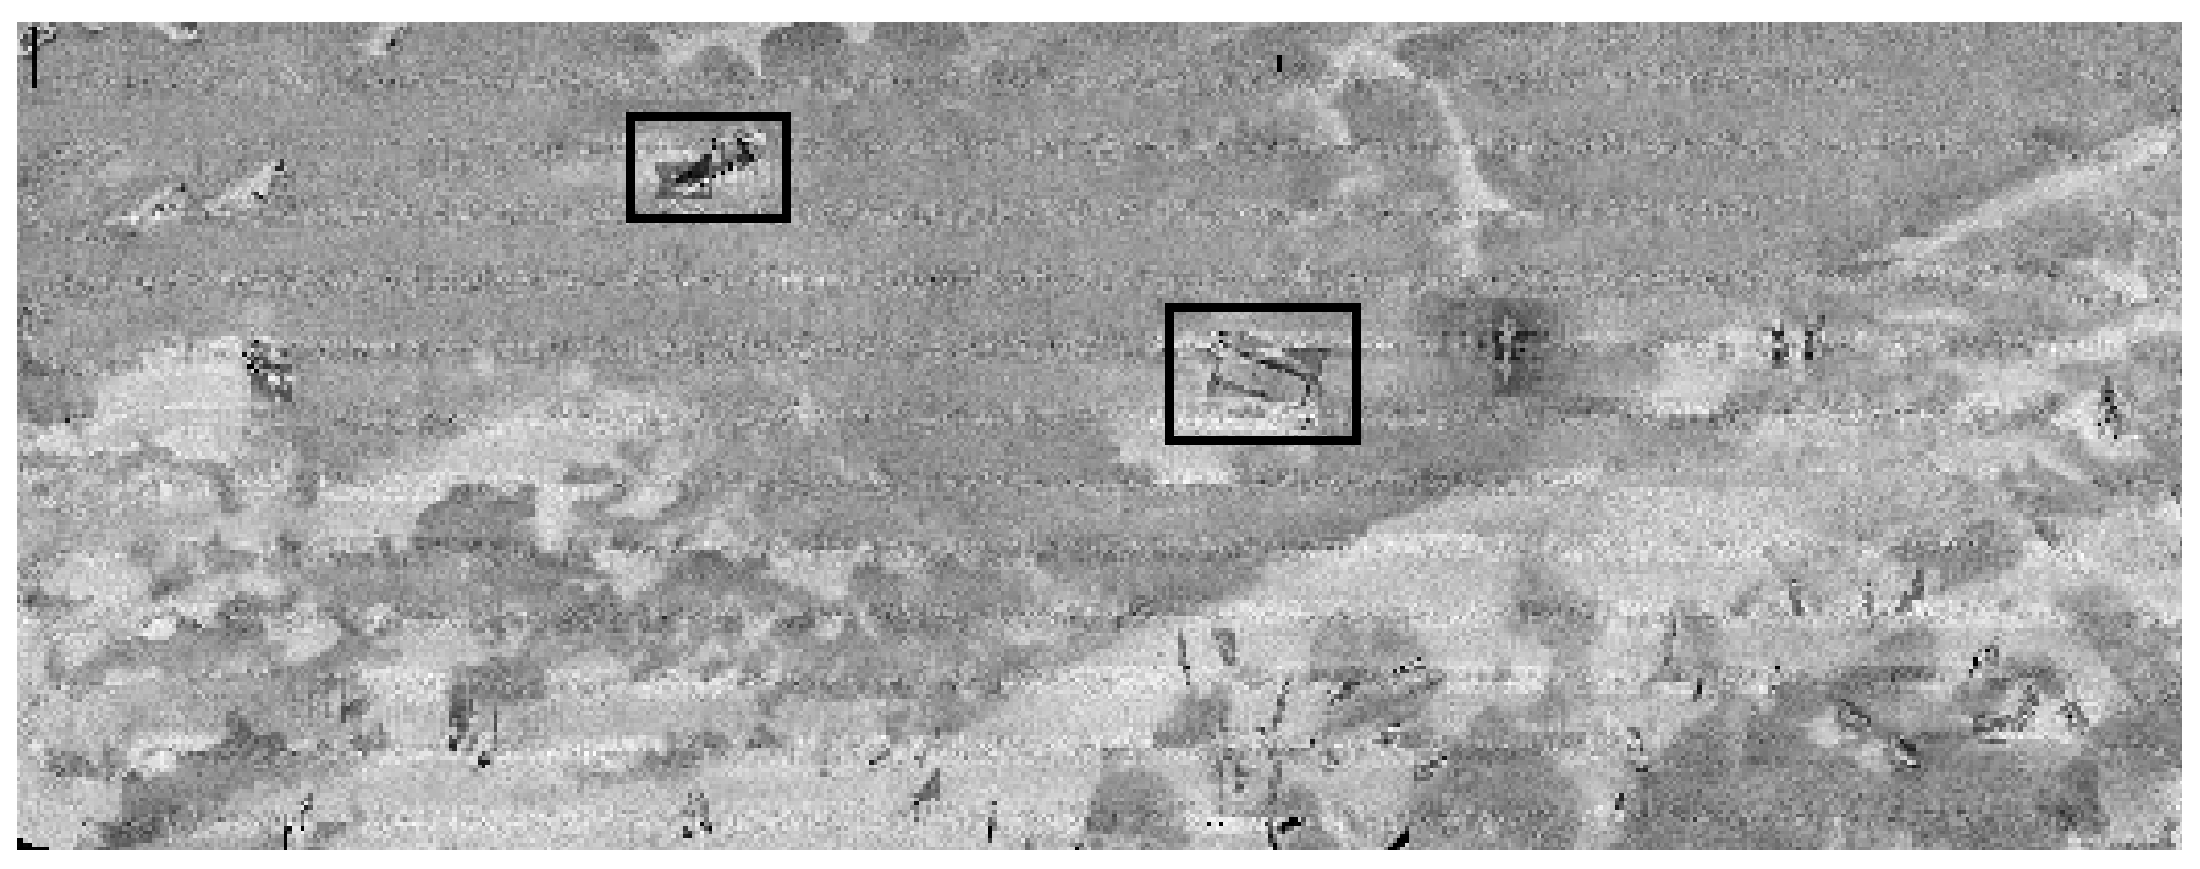
\includegraphics[width=\textwidth]{subwayorig}
      \caption{Backscatter image of sea-floor from Gavia AUV}
      \label{subfig:subwayorig}
  \end{subfigure}
  \begin{subfigure}[]{0.9\textwidth}
      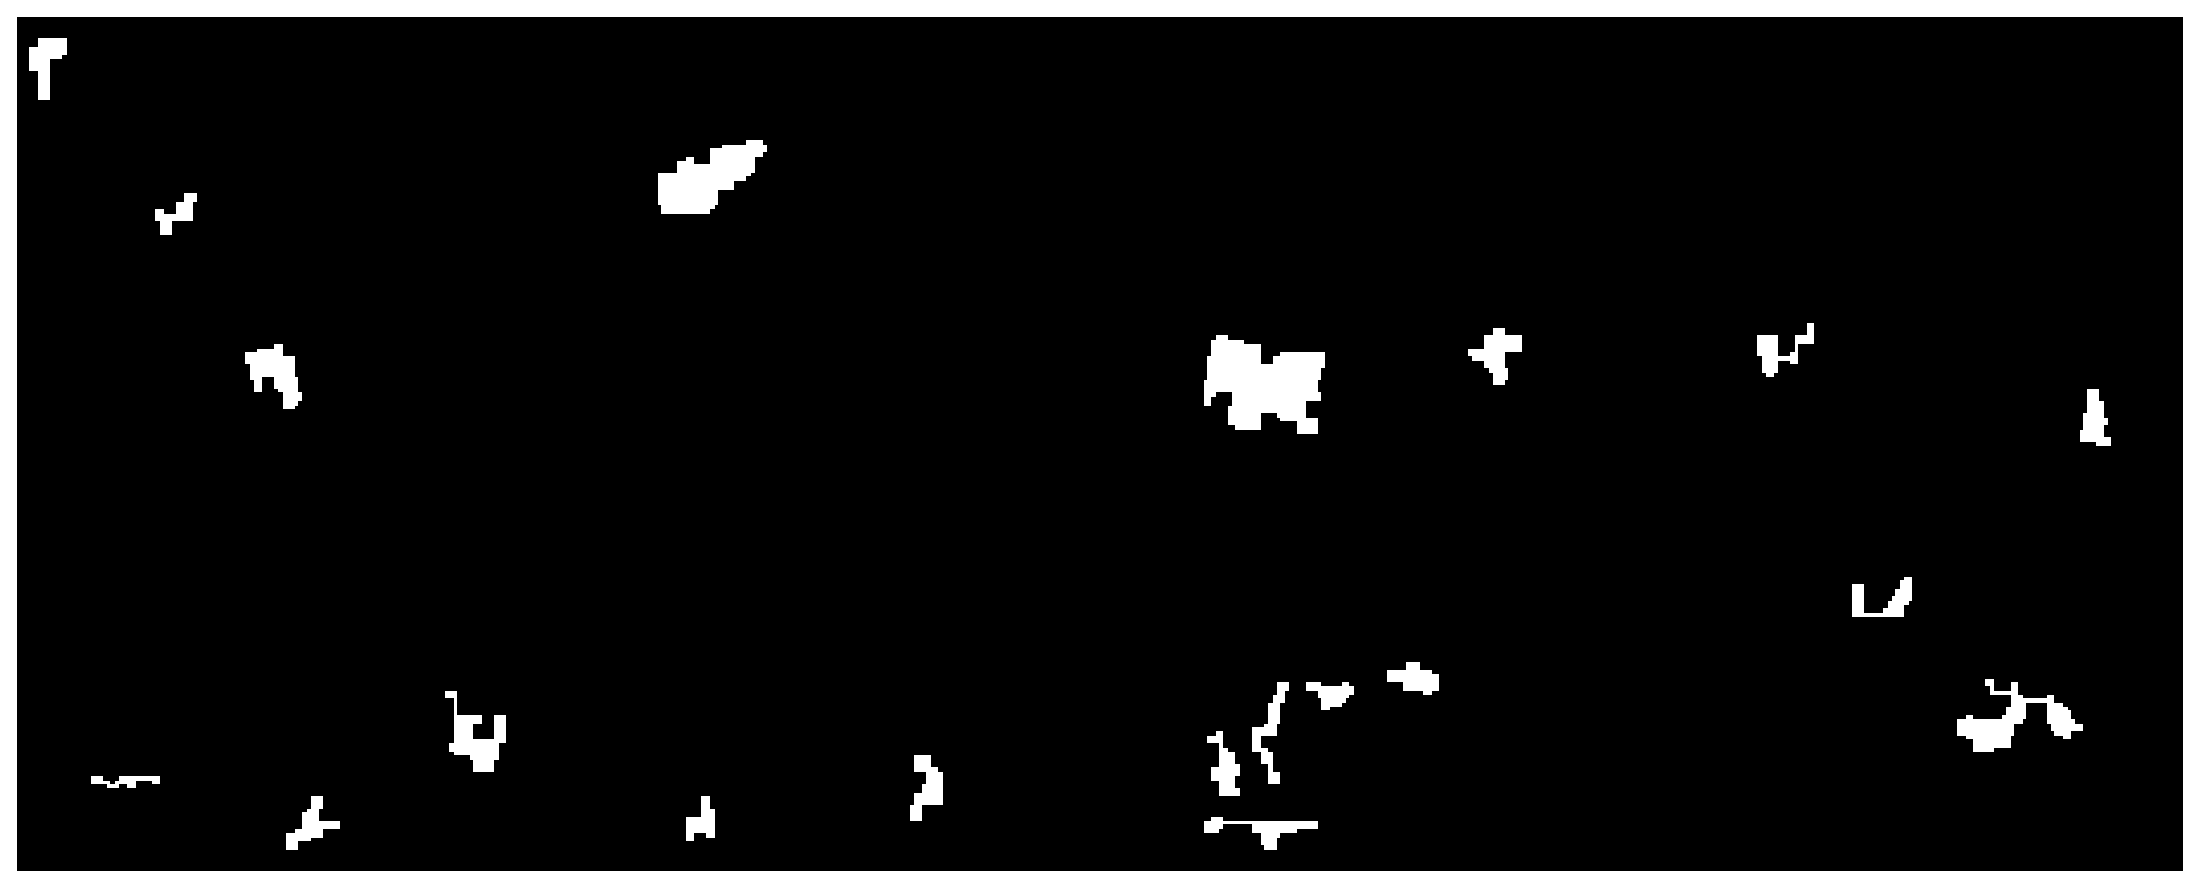
\includegraphics[width=\textwidth]{subwaysegment}
      \caption{Image segmentation using basic morphological operations and edge detection}
      \label{subfig:subwaysegment}
  \end{subfigure}
\caption[Analysis of sonar backscatter image of Redbird reef]{}
\end{figure}

The sonar backscatter image of Redbird reef in Figure~\ref{subfig:subwayorig} shows the shape profiles of some sunken objects resting on the seabed. Two subway cars are marked using black rectangles. If we look for rectangular objects like the rectangle in Figure~\ref{subfig:subwayrect}, it is likely that eigen-value shape descriptors will distinguish the profiles of subway-cars, as there are no other objects with such rectangular shape profile in the seabed image (Figure~\ref{subfig:subwayorig}). 

\begin{figure}
    \centering      
    
\includegraphics[width=0.4\textwidth]{eigenrect}
    \caption[Rectangular template used as reference shape for subway-cars]{Rectangular template used as reference shape for subway-cars}
    \label{subfig:subwayrect}
\end{figure}
%
\begin{figure}
    \centering
    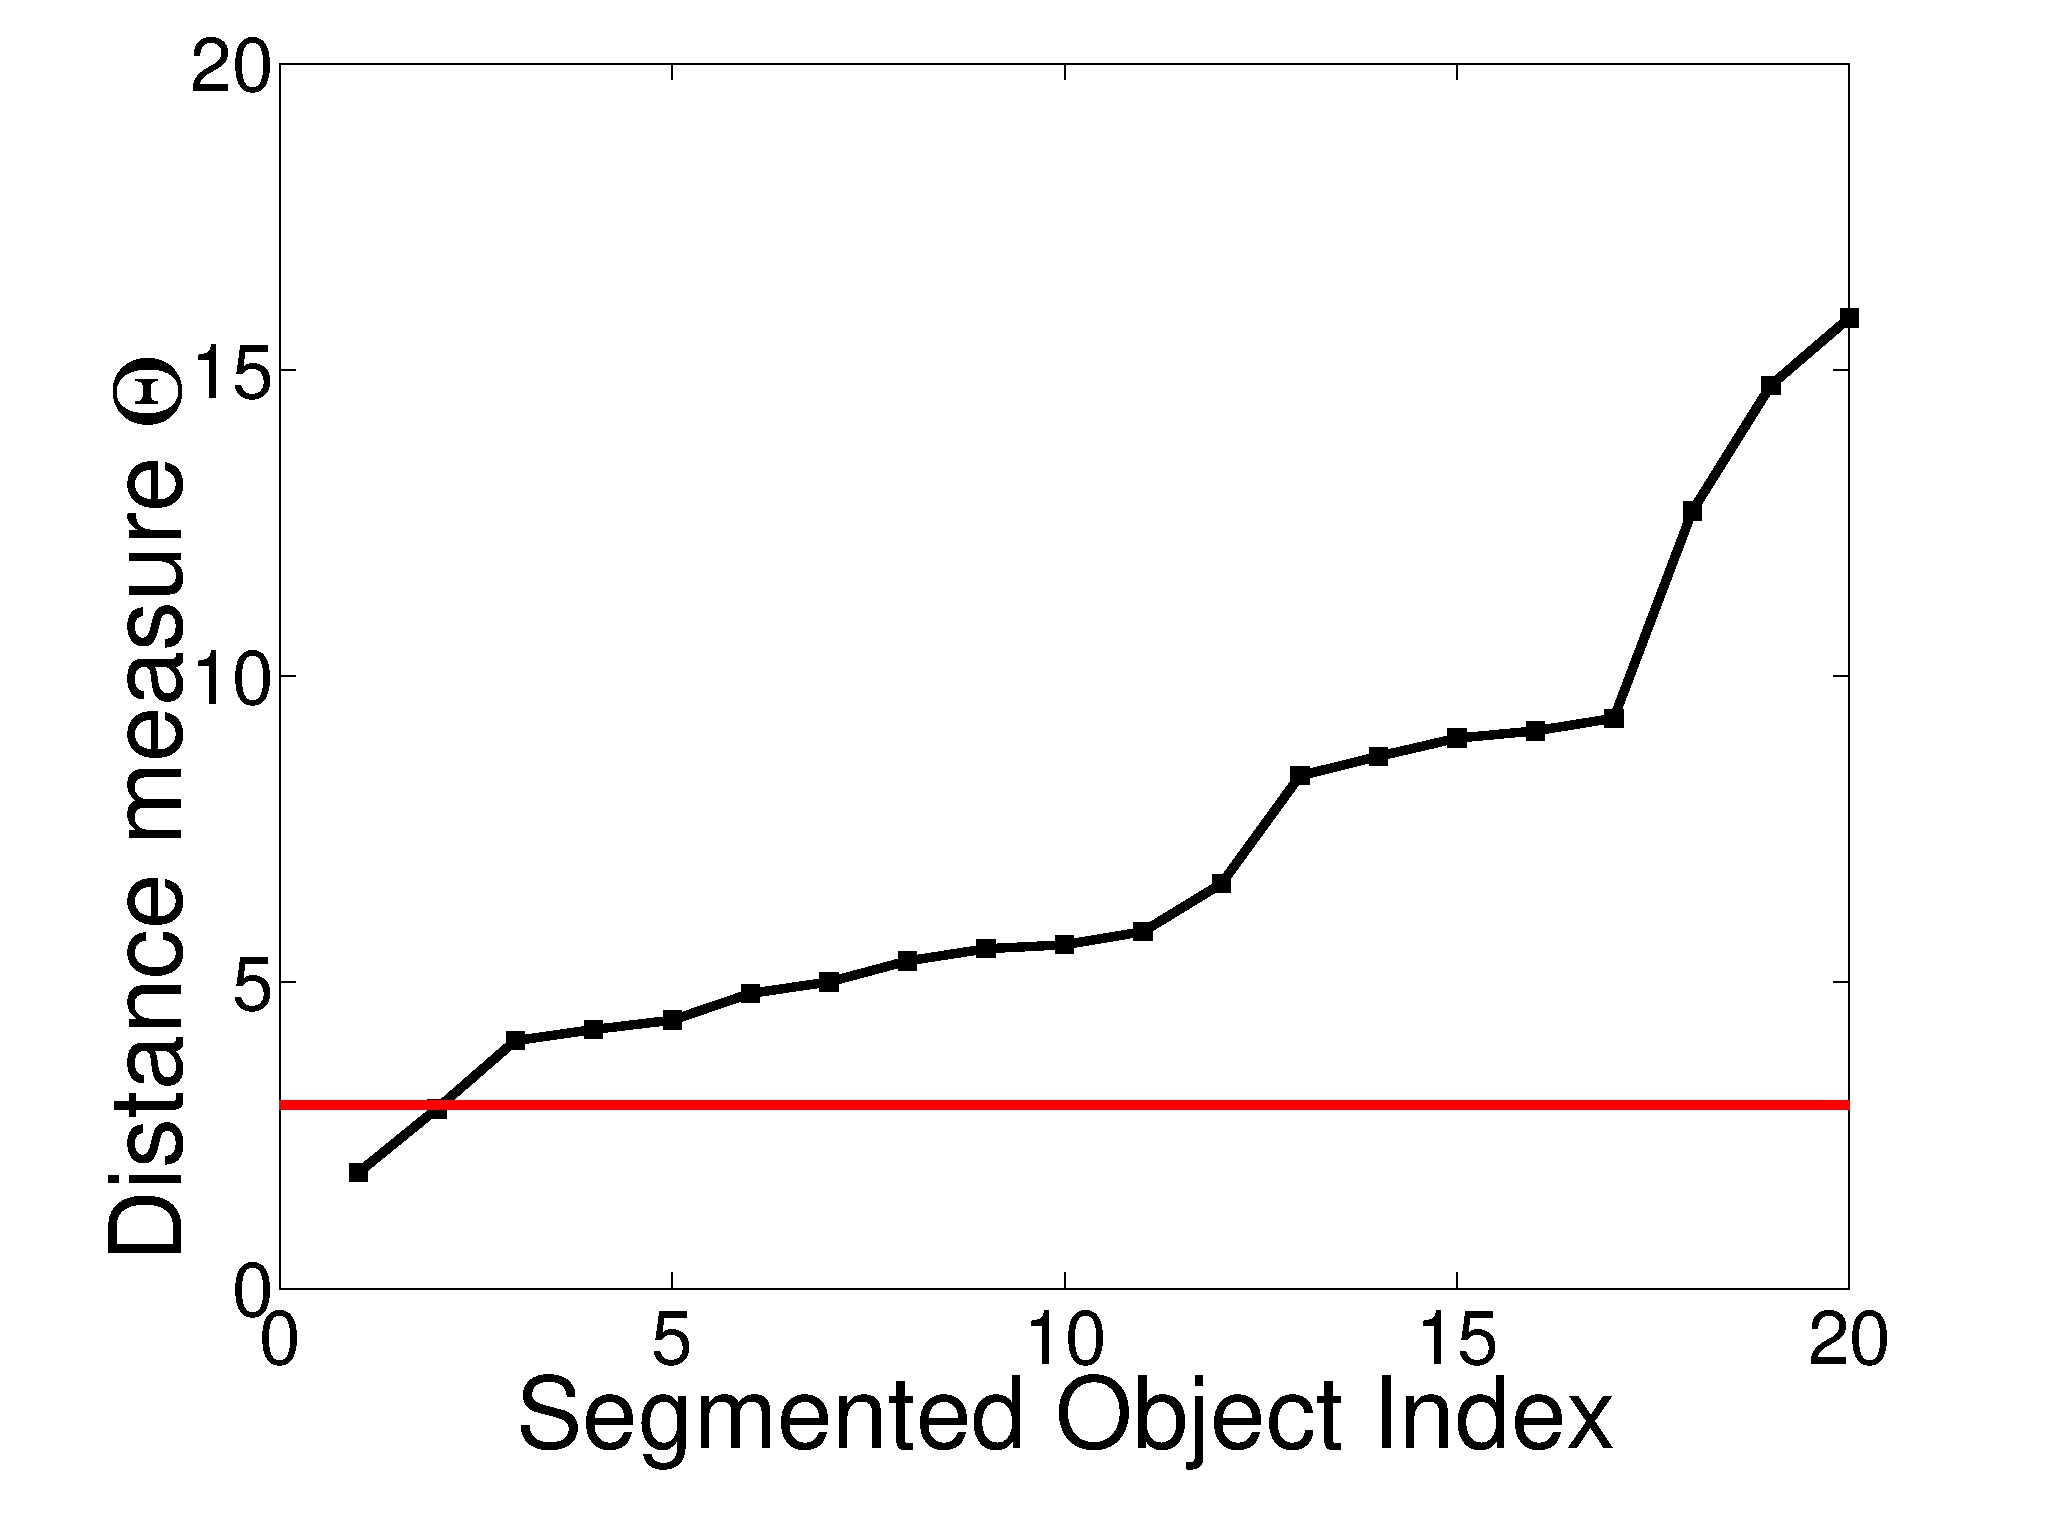
\includegraphics[width=0.8\textwidth]{subway_dot_prod}
    \caption[Plot of similarity measures of different underwater objects to the subway car reference profile]{Plot of the weighted distance D between each segmented feature and the template rectangle in Figure~\ref{subfig:subwayrect}. The threshold (D=3) is shown as a red line.}
    \label{subfig:eigendistances}
\end{figure}

In order to verify the ability of eigen-value shape descriptors to pick out the subway-cars in Figure~\ref{subfig:subwayorig}, we follow a sequence of steps. The sonar backscatter image is first segmented to get a series of shape profiles using a grayscale threshold operation on the image. Figure~\ref{subfig:subwaysegment} shows the different ``blobs'' obtained after thresholding. The blobs were then compared to the rectangular shape in Figure~\ref{subfig:subwayrect} using the angle $\Theta$ metric that was defined in \eqref{eq:eigendist}. The $\Theta$ value of a blob is a direct indicator on how close in appearance it is to the reference rectangle in Figure~\ref{subfig:subwayrect}. The smaller the $\Theta$ value, the closer it is in appearance to the reference rectangle shape $\Omega_r$. The $\Theta(\Omega_r,\Omega_j)$ value for each blob $j$ is recorded and the $\Theta$ values are plotted in ascending order in Figure~\ref{subfig:eigendistances}. 

The two blobs that correspond to subway cars have the lowest $\Theta$ values. The blob with the lowest $\Theta$ value ($\Theta=1.89^{\circ}$) along with its plotted shape descriptor $F$ is shown in Figure~\ref{subfig:subwaybest1}. Similarly the blob with the second lowest $\Theta$ value is shown in Figure~\ref{subfig:subwaybest2}($\Theta=2.93^{\circ}$). In Figures~\ref{subfig:subwaybest1} and ~\ref{subfig:subwaybest2}, the blue line corresponds to the shape descriptor $F(\Omega_r)$ of reference rectangle $\Omega_r$ and the red line corresponds to the shape descriptor $F(\Omega_j)$ of blob $j$. The $\Theta(\Omega_r,\Omega_j)$ is the computed angle between the shape descriptor vectors as discussed in \eqref{eq:eigendist}. In contrast, the blob with the largest $\Theta$ value ($\Theta=15.85^{\circ}$) or in other words the blob that matches the least with the reference rectangle is shown in Figure~\ref{subfig:subwayworst}. In this case, if we set a threshold $\Theta_{thresh}=3$ and only consider objects with $\
Theta<\Theta_{thresh}$ to 
be subway cars, then we have a mechanism to detect subway cars from other objects present in this sonar image. This effectively shows that eigen-value shape descriptors are in principle capable of picking up prespecified shapes from images.

\begin{figure} 
  \centering
  \begin{subfigure}[]{0.45\textwidth}
      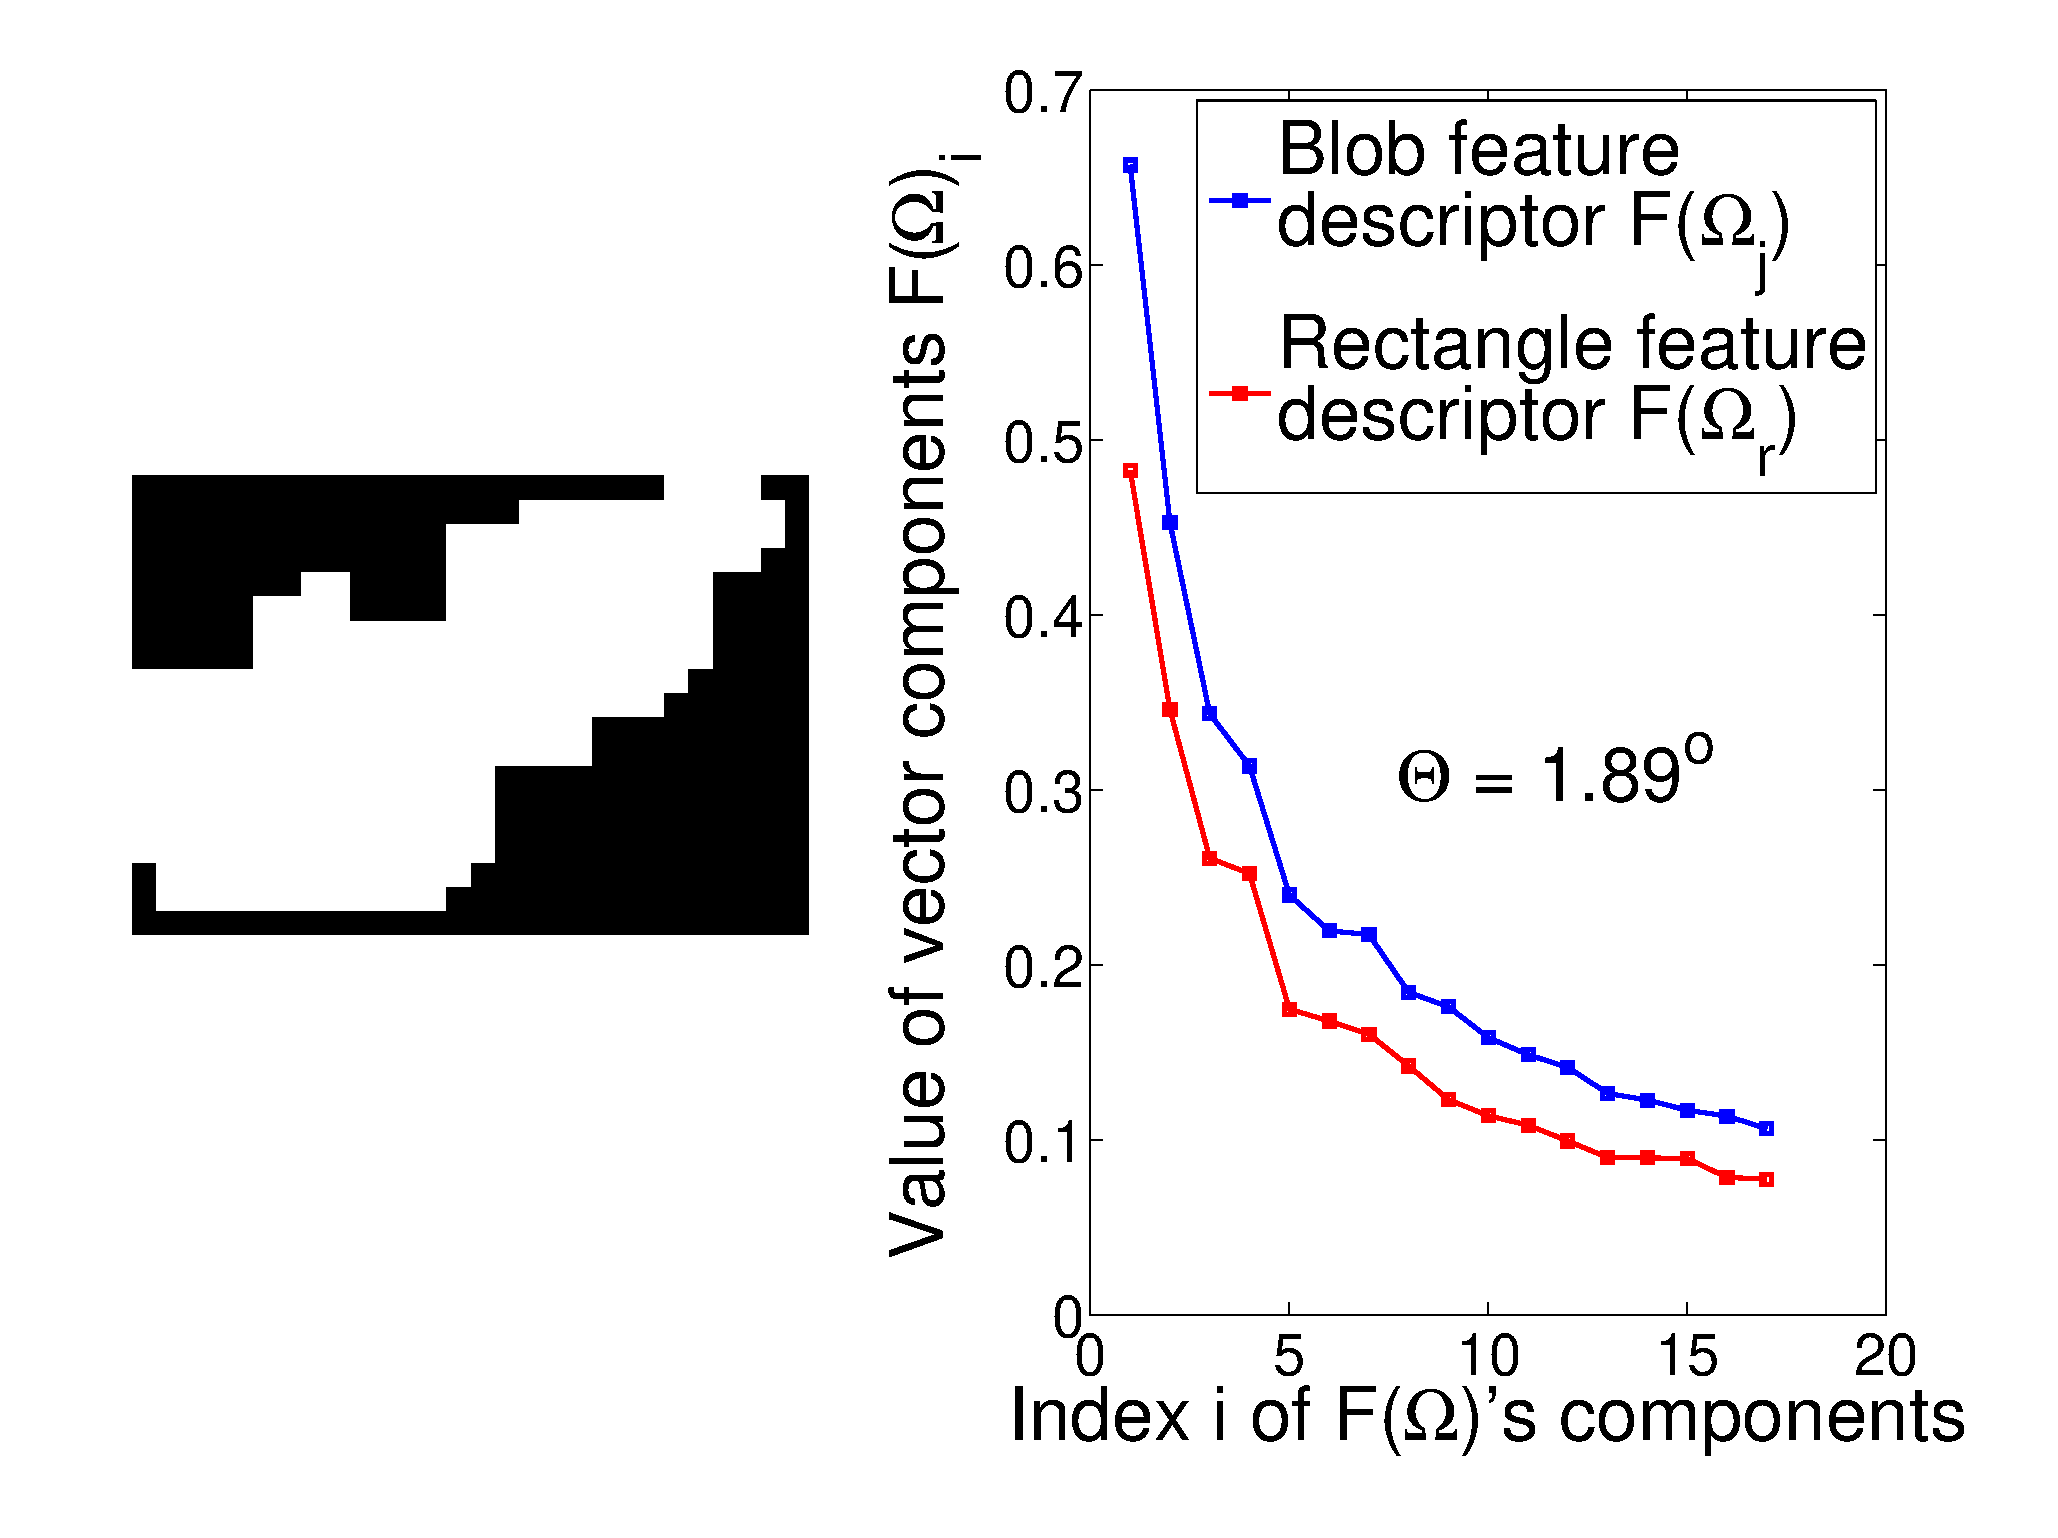
\includegraphics[width=\textwidth]{best1}
      \caption{}
      \label{subfig:subwaybest1}
  \end{subfigure}
  \begin{subfigure}[]{0.45\textwidth}
      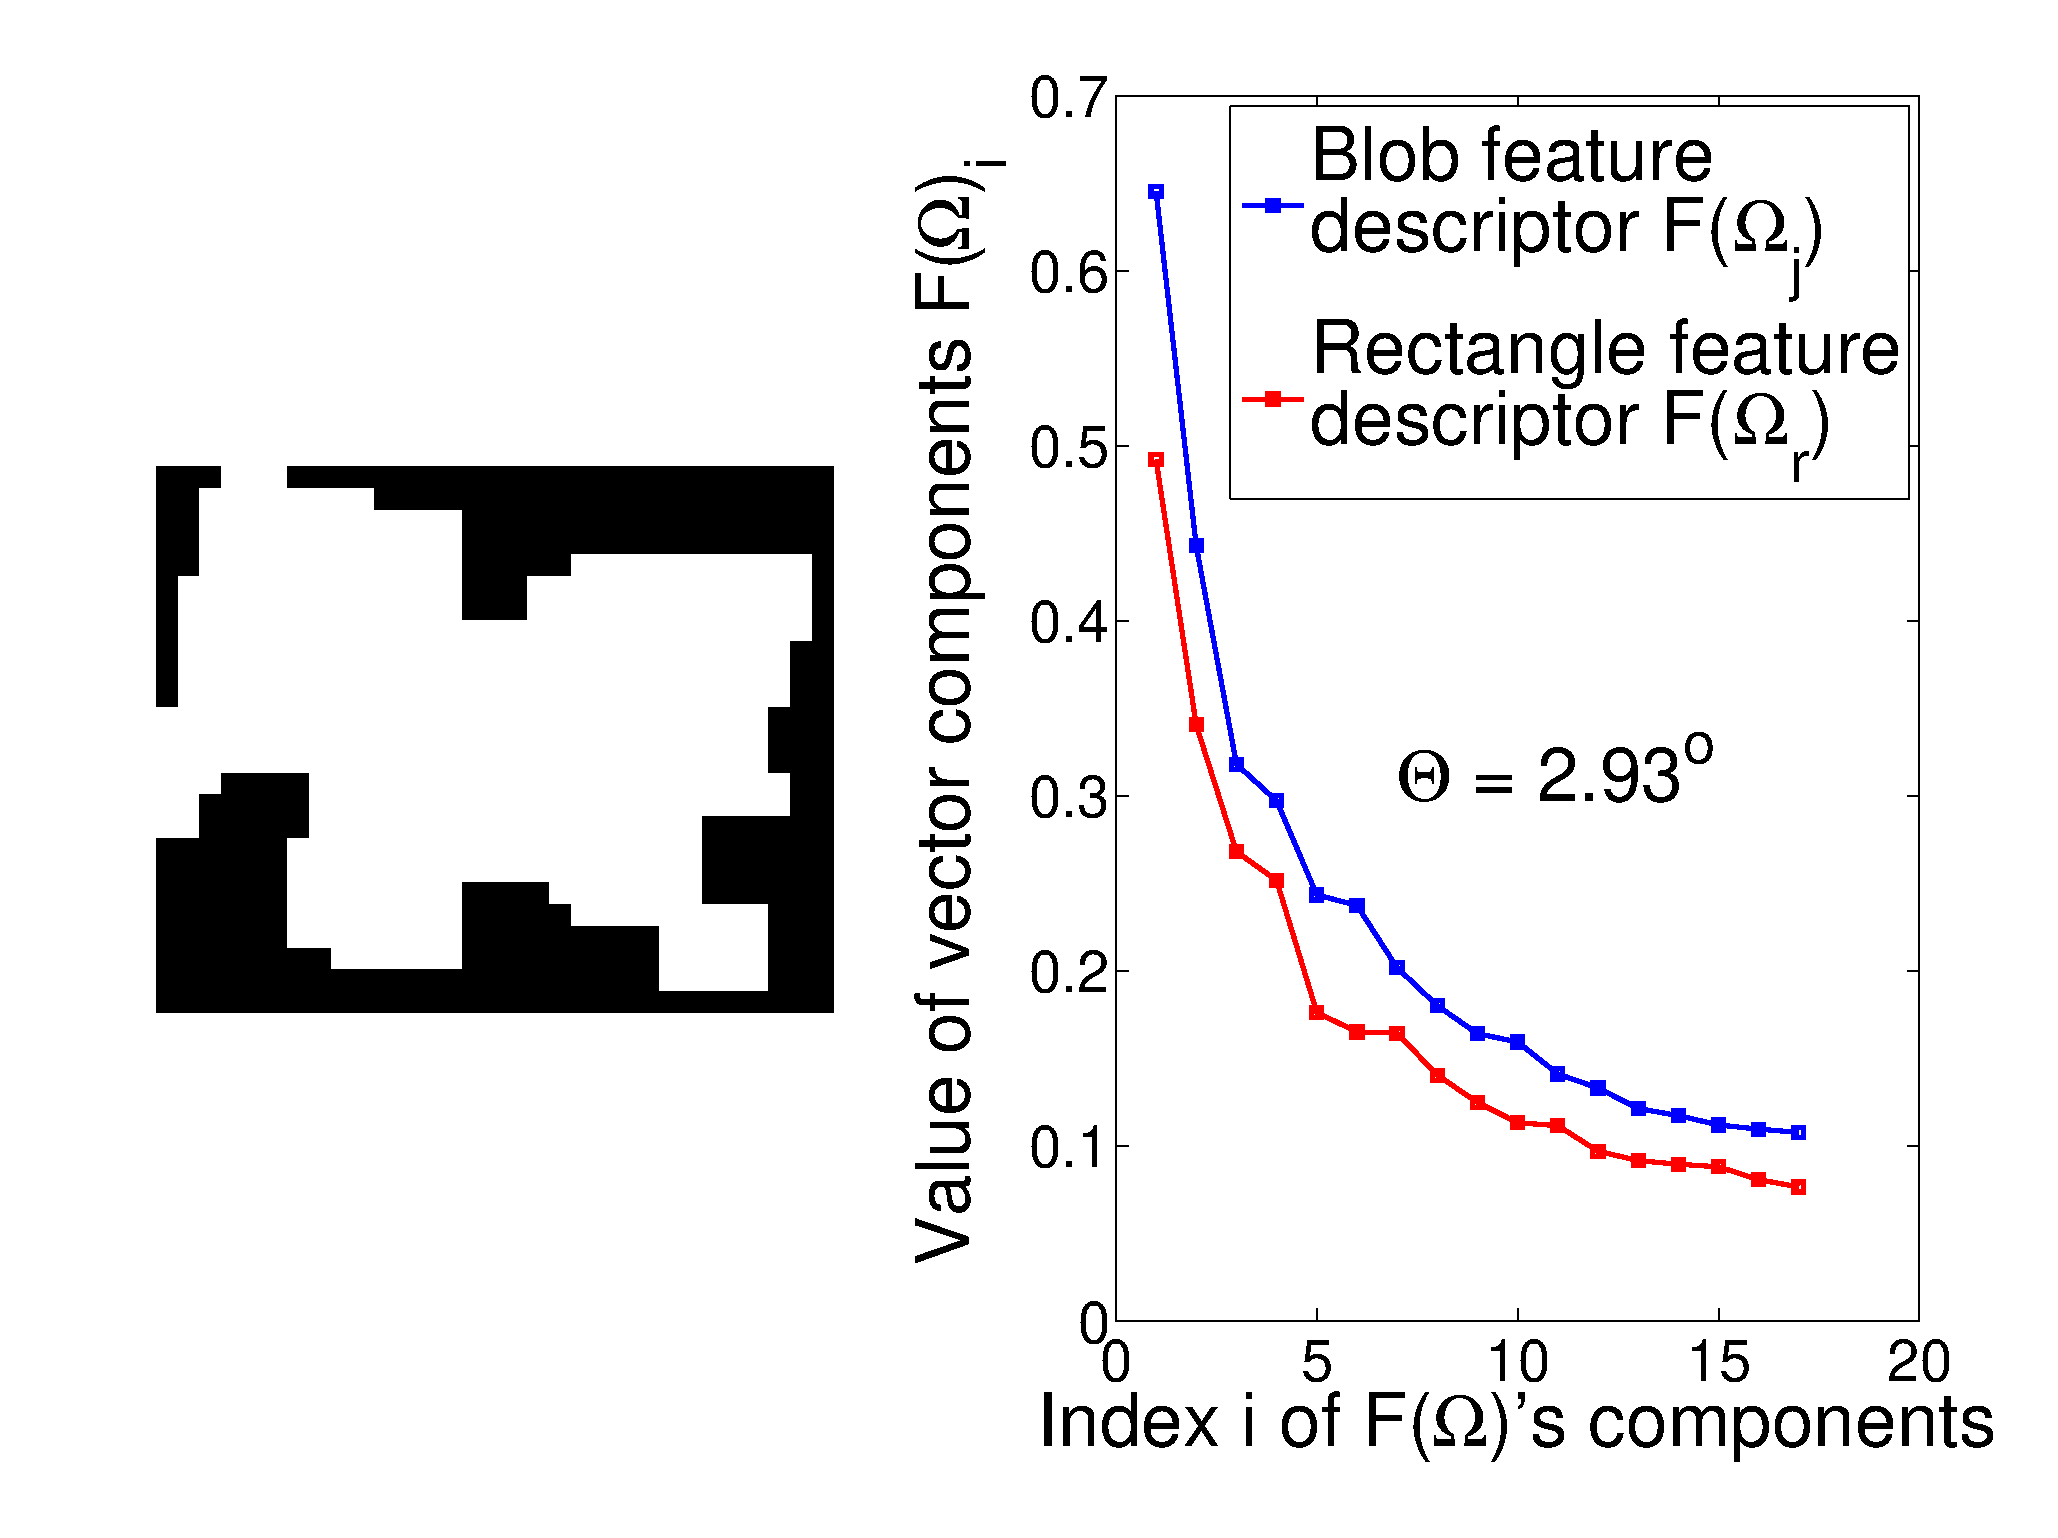
\includegraphics[width=\textwidth]{best2}
      \caption{}
      \label{subfig:subwaybest2}
  \end{subfigure}
  \begin{subfigure}[]{0.45\textwidth}
      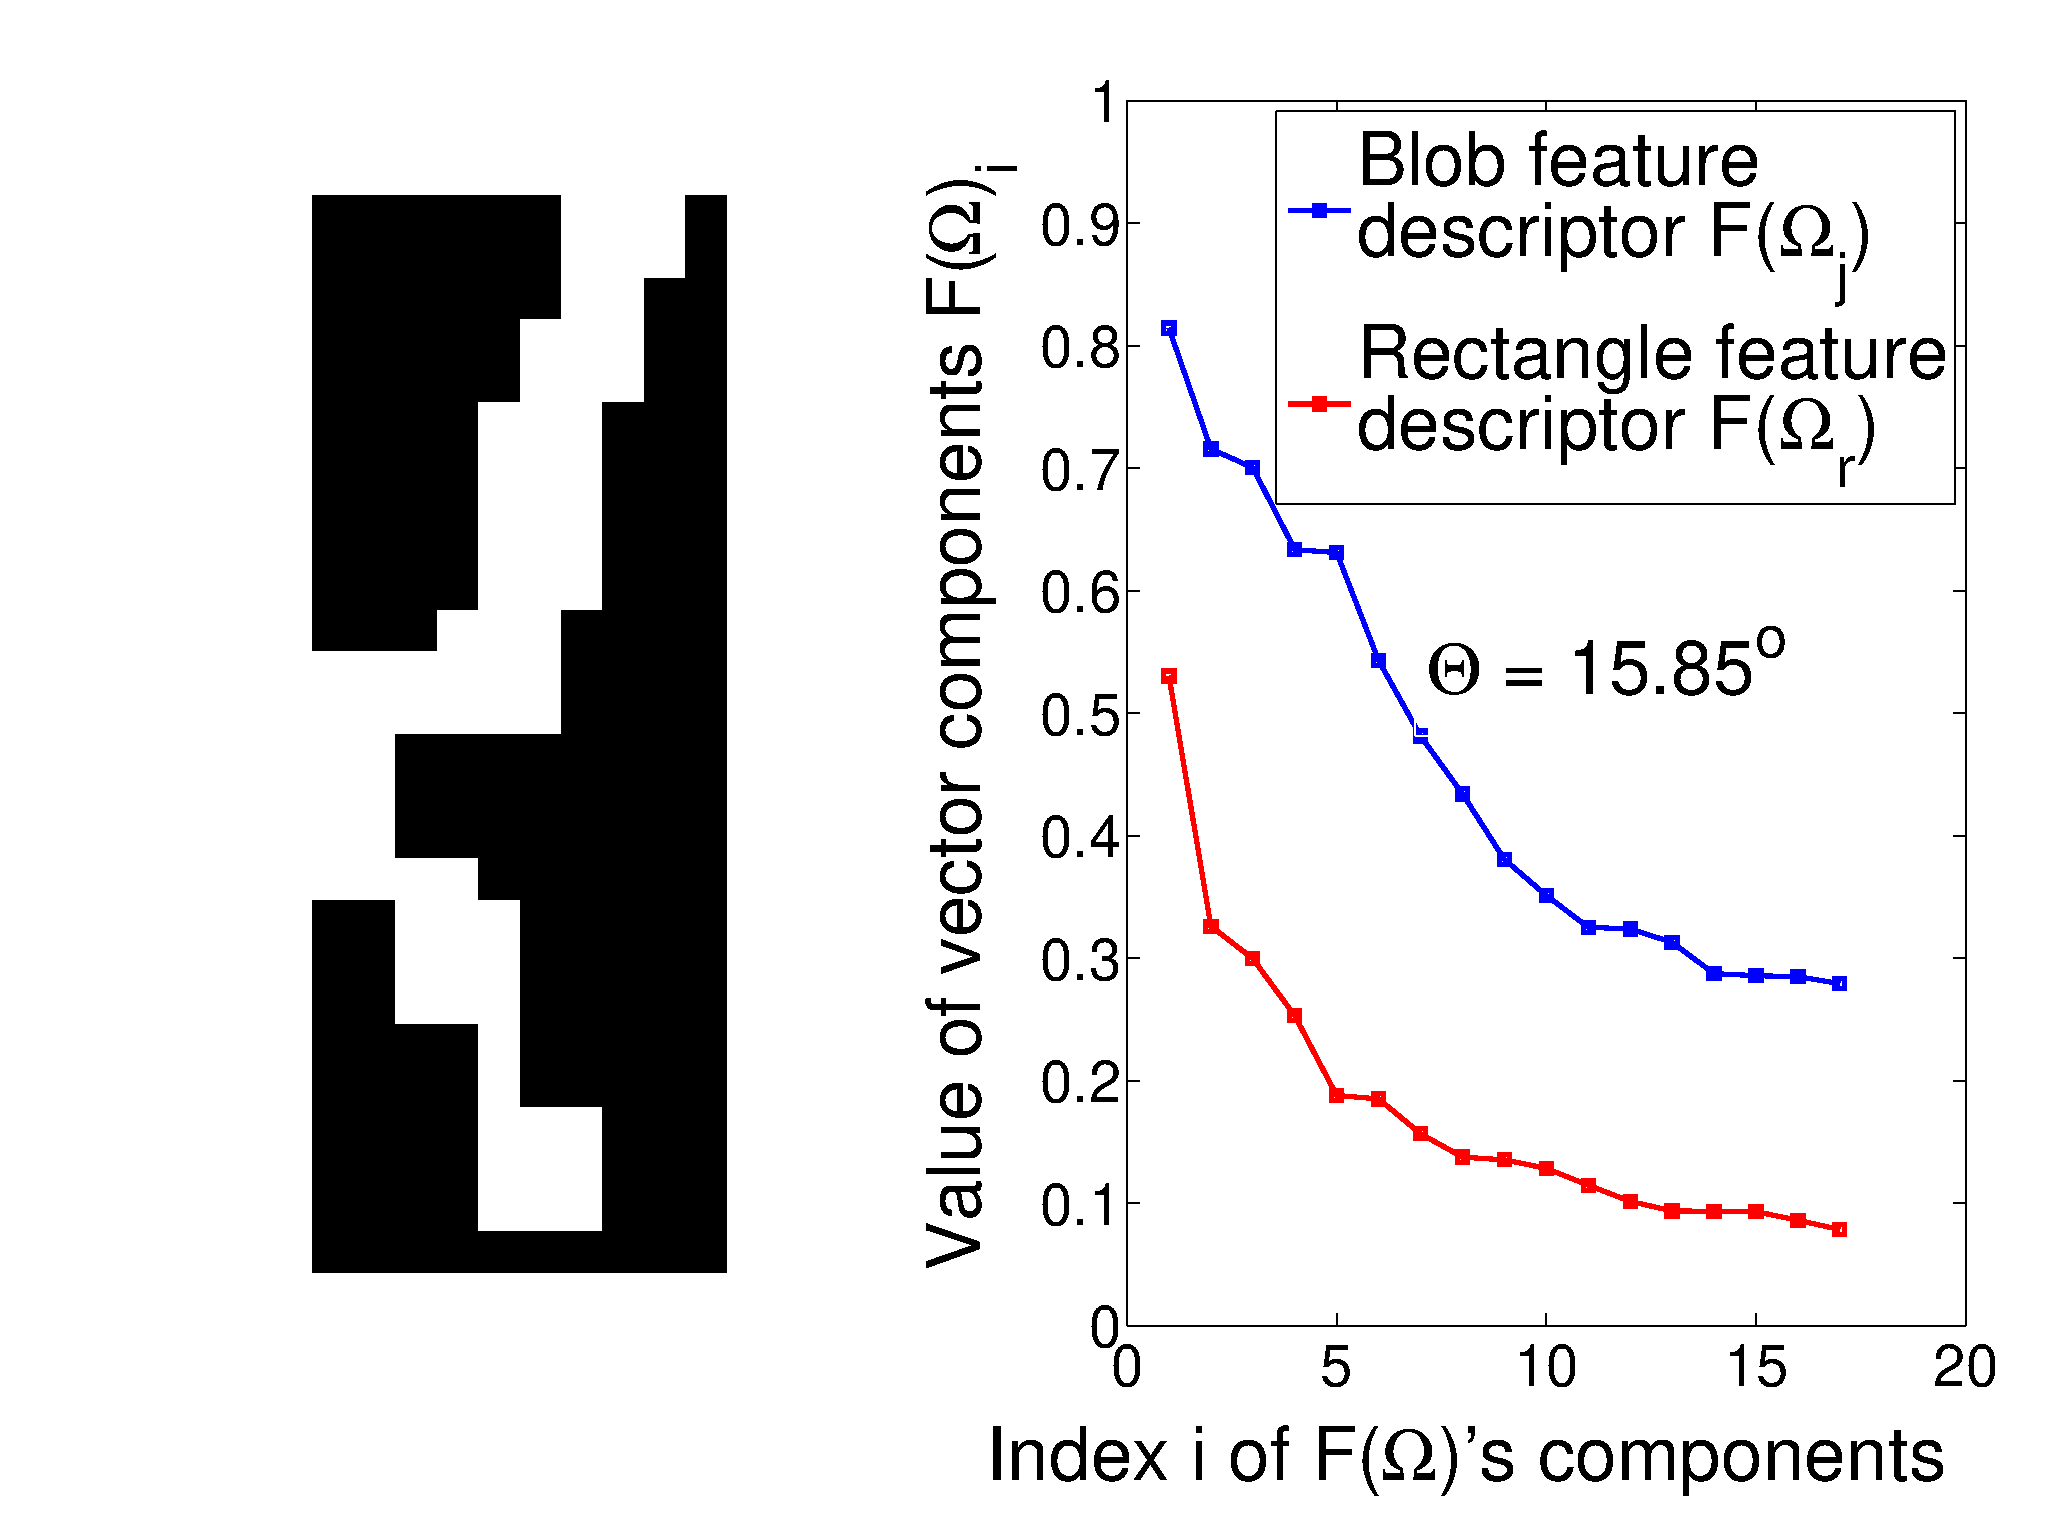
\includegraphics[width=\textwidth]{worst1}
      \caption{}
      \label{subfig:subwayworst}
  \end{subfigure}
\caption[Subway car recognition results]{Parts (\subref{subfig:subwaybest1}) and (\subref{subfig:subwaybest2}) correspond to the blobs that are closest to the reference rectangle in Figure~\ref{subfig:subwayrect}. The shape of the blob $j$ is shown on left and the corresponding plot of shape descriptor $F(\Omega_j)$ (red line) along with the plot of the reference rectangular profile (blue line) is shown on right. The distance measure $\Theta$ between the blob and the reference rectangle gives a picture of how close the given blob is to the reference rectangle. A contrasting view of the blob that matches the least with the reference rectangle is shown in (\subref{subfig:subwayworst}).}
\end{figure}      


\section{Discussion}

In Section~\ref{sec:subwaycar_results}, we saw how eigen-value shape descriptors can be utilized to detect subway cars from other underwater objects. The eigen-value shape descriptors here were tuned to look for rectangular objects that match the profile in Figure~\ref{subfig:subwayrect}. The blobs obtained as matches to the reference rectangle through this eigen-value shape descriptor method complies with the ground truth information on the position of the subway cars in the sonar image (Figure~\ref{subfig:subwayorig}). Hence from this study, we see that eigen-value shape descriptors provide a viable mechanism to detect objects with specific shapes.

Since eigen-value shape descriptors purely rely on the shape of an object, two objects with identical shapes but significantly different textures cannot be differentiated using this method. In tests we performed, eigen-value descriptor did not perform well on objects whose shape is characterized by more complex contours. For instance when eigen-value shape descriptors were evaluated as a tool to recognize numbers between 0 and 9, 1 and 7 were often confused and wrongly classified. Similar misclassifications were also registered between 0,6,8 and 9. These errors can be attributed to the \gls{rst} invariance property coupled with discretization errors while representing numbers (0-9) in an image form. Even though \gls{rst} invariance is helpful in some cases, it can be detrimental when the orientation of a shape can play a part in the recognition process. The theoretical mechanism behind the eigen-value shape descriptors defines it over a continuous domain. When eigen-value shape descriptors were adopted as a 
shape 
identification tool on images, the domain needed to be discretized; images are nothing but discrete spatial arrangement of pixel values. When dealing with complex shapes, there can be significant discretization errors that can adversely affect the performance of eigen-value shape descriptors. High levels of noise and errors in segmentation are other significant factors that can lower the performance of eigen-value shape descriptors.


\section{Conclusion}

Eigen-value based shape identification is a tool that can be used to identify simple predefined shapes from natural images. This method was successful in identifying subway-cars from sonar images of the seabed under the assumption that subway cars are rectangular in shape. Apart from shape, the texture of an object plays a key role in determining the identity of an object. Since eigen-value shape descriptors discard textural information, they are not suited for applications where shape is insufficient to decipher the identity of an object. Additionally, while dealing with complex shapes, there can be significant discretization error, and also segmentation errors which can affect the shape profile of an object. Such errors often diminish the performance of eigen-value shape descriptors. Hence eigen-value shape descriptors is a useful tool for identifying objects provided we can guarantee that the shape of the object can be described in a discrete domain with minimal error. Furthermore, for this method to work,
 the 
objects we are interested in should exhibit a shape profile that is significantly different from all other objects in the background. 

Natural objects, like marine organisms, are typically associated with complex shape profiles. Furthermore texture is often a key discriminant required to identify marine organisms. The inability to use textural information, among other factors, limits eigen-value shape descriptors to few specialized object recognition applications only. Chapter~\ref{chap:scallop_recog} offers a multi-layered object recognition solution that attempts to overcome some drawbacks seen in eigen-value shape descriptor approach.

%========================================================================================


%=========================================================================================
% Chap4: Literature review on underwater animal detection

\chapter{Underwater Animal Recognition}
\label{chap:animal_lit}

\section{Introduction}

In natural settings, living organisms often tend to blend into their environments to evade detection via camouflage. Webster's thesis work \cite{webster} provides a detailed exposition on the visual camouflage mechanisms adopted by animals to blend into their background. Under such circumstances of camouflage, there are very limited visual cues that can be used to identify animals. Even in the presence of visual cues, the task of identifying animals from natural scenes is shown to be a cognitively challenging and complex task \cite{wichmann}.

There is an extensive body of literature related to identifying marine animals. Some of this work is specialized for identifying different types of animals under specific environmental conditions. In general, the existing methods can be broadly divided into methods devised for identifying mobile organisms and methods for sedentary organisms. The former category is useful in dealing with a wide range of sea organisms like the varied species of fish that swim through water. The latter category is less studied. It includes identifying sedentary marine animals like scallops, corrals and sponges. Both categories present their own set of challenges. In the rest of this chapter we visit the techniques relevant to moving animals and show how they are different from the methods employed for sedentary animals. An overview of the existing literature on recognizing sedentary animals follows, with special emphasis on methods developed for identifying scallops. The shortcomings of the 
existing methods in recognizing sedentary underwater animals is addressed through a multi-layered method discussed in Chapter~\ref{chap:scallop_recog}.

%========================================================================================

\section{Methods for Recognition of Moving Underwater Organisms}

Recognizing and counting mobile marine life like fish~\cite{spampinato, edgington, williams} and studies in aquaculture \cite{zion} have been attempted. The recurring theme in these efforts involves the use of stationary cameras to detect the presence of moving species, provided that the background can be described by a prior model. This technique of assuming a known background, and using changes in the background as an evidence for the presence of a moving object entering the field of view of a sensor, is called background subtraction. In the marine species identification case, any changes to the background are assumed to be caused by a moving marine organism. The pixels in the image that deviate from the background model can be labeled as the pixels belonging to the organism.

Once a marine organism is detected through background subtraction, then other computer vision or machine learning techniques can be used to classify the organism into a specific species based on its visible characteristics. This classification task can be achieved through conventional machine learning approaches. For instance the salmon species classification algorithm developed by Williams et al. \cite{williams} uses active contours to model the shape of the fish before comparing these contours to known salmon species. However, if the pixels corresponding to the organism are contaminated by high levels of noise, a specialized technique that is robust to noise might be required.

Background subtraction requires a mathematical model that describes the distribution of background pixels. In an underwater setting, such a background model can only be obtained if the camera is stationary and is observing a static background, or in the case that the background model represents , the evolution of which over time can be captured through a mathematical model. Such well defined background models are not always available. An opportunity to employ the background subtraction-based techniques arises in underwater environments with stationary fixtures designed to study a specific underwater location. In instances where such stationary arrangement of cameras is not available, background subtraction is inapplicable due to the lack of a background model.

%========================================================================================

\section{Methods for Recognition of Sedentary Underwater Organisms}

Since sedentary marine animals like scallops do not typically move (unless chased by a predator), a mobile robotic platform is required to traverse subsea relief to image and recognize those marine animals. Extending background subtraction to work with mobile robotic platforms is challenging, since the motion of the platform causes changes in its background. Generating a model for the background to perform background subtraction in these cases is problematic. This makes the task of detecting sedentary organisms with moving sensors even more challenging than detecting moving organism with stationary sensors. The lack of background model in these cases motivates the development of a foreground model. If a foreground model is available, the task of detecting an organism can be realized as a search for pixels satisfying the foreground model in the image.

Detecting an organism typically involves segmenting all pixels of the organism, in order for one to classify the organism into a known category. 
The motion-based segmentation of marine animals that involves subtracting a known model of background from a snapshot of the environment, followed by attributing the pixels with non-zero values to the foreground is inapplicable in cases where the background model does not exist. 
Furthermore, the task of segmentation can be challenging in noisy images with weak edges, since the boundary pixels of the foreground object cannot be easily distinguished from background pixels.

Thus, the lack of background model makes background subtraction problematic. This leads to the need for techniques that depend on foreground models, and use of other features to detect and segment organisms from the background. This task becomes even more complicated if the organism does not present significant visual cues that make it distinctive from the background, as in the case of creatures exhibiting camouflage. High levels of noise or unpredictable environmental variables could also significantly affect the effectiveness of any animal recognition mechanism.

%========================================================================================

\section{Scallop Recognition}

Previous efforts to detect animals like plankton~\cite{mcgavin_plankton, stelzer_rotifier}, clam~\cite{forrest_clam} and a range of other benthic megafauna~\cite{schoening} exist. Most of these methods here are specialized to a specific species, or only tested in controlled environments. In some cases, the methods require specialized apparatus (like in the plankton recognition studies~\cite{mcgavin_plankton, stelzer_rotifier}). 
A series of automated tools like specialized color correction, segmentation and classification modules along with some level of manual expert support, can be combined identification of several marine organisms like sea anemones and sponges from natural image datasets~\cite{schoening}. 

There are several aspects that make scallop recognition challenging.
Scallops, especially when viewed in low resolution, do not provide features
that would clearly distinguish them from their natural environment.  This
presents a major challenge in designing an automated identification process 
based on visual data.  To compound this problem, visual data collected
from the species' natural habitat contain a
significant amount of speckle noise.
Some scallops are also partially or almost completely
covered by sediment, obscuring the scallop shell features.
A highly robust detection mechanism is required to overcome these impediments.

There is a range of previously developed methods specialized for scallop recognition 
\cite{dawkings13,guomundsson,enomoto9,enomoto10,fearn, prasanna_med, prasanna_aslo, prasanna_igi} 
that operate on different assumptions, either with regards to the environmental conditions or the quality of data.
Existing approaches to automated scallop counting in artificial environments
 \cite{enomoto9, enomoto10} employ a detection mechanism based on intricate distinguishing features 
like fluted patterns in scallop shells and exposed shell rim of scallops, respectively.
Imaging these intricate scallop shell features might
be possible in artificial scallop beds with stationary cameras and 
minimal sensor noise, but this level of detail 
is difficult to obtain from low resolution images of scallops in their natural environment. 
A major factor that contributes to the poor image resolution is the fact that sometimes the image of a target
is captured several meters away from it. 
Overcoming this problem by operating an underwater vehicle much closer to the ocean floor 
will adversely impact the image footprint (i.e. area covered by an image) and increase the risk of damaging the vehicle.

Furthermore,  existing work on scallop detection \cite{dawkings13, guomundsson} in their natural
environment is limited to small datasets (often less than 100 images). 
A sliding window approach has been used \cite{guomundsson} to focus the search for the presence of scallops. The large number of overlapping windows that need to be processed per image raises scalability concerns if this method were to operate 
on a large dataset containing millions of images. Additionally, the small number of natural images used as a test set raises questions about the generalizibility of this method and its ability to function under varied environmental conditions.
The work by Dawkins \cite{dawkings13} is more detailed in its treatment of the natural environmental conditions spanning the scallop habitat. The images used here are collected using a towed camera system that minimizes noise, a fact which greatly enhances the performance of the machine learning and computer vision algorithms. Despite the elaborate imaging setup designed to minimize noise, the results reported are derived only from a few tens to hundreds of images.
It is not clear if those machine learning methods \cite{dawkings13} can extend to noisy image data captured by \gls{auv}s.
From these studies alone, it is not clear if such methods can be used effectively
in cases of large datasets comprising several thousand seabed images.
An interesting example of machine-learning methods applied to the
problem of scallop detection \cite{fearn} 
utilizes the concept of \gls{buva}.
The approach is promising but it does not use any ground truth for validation.  

There is more work \cite{prasanna_med, prasanna_aslo, prasanna_igi} that offers a multi-layered object recognition framework validated on
a natural image dataset for scallop recognition application. 
The main emphasis there (and in this dissertation) is to develop a technique that can work on low quality noisy sensor data collected using \gls{auv}s.
The other objective is to build a scalable architecture that can operate on 
large image datasets in the order of thousands to millions of images
and can be generalized for recognizing other marine organisms.
A detailed account of this multi-layered approach is discussed in Chapter~\ref{chap:scallop_recog}.

%========================================================================================

\section{Applicability of Existing Methods for Scallop Recognition}

Existing methods for recognizing moving underwater organisms like fish depend on background subtraction. Though background subtraction 
offers a convenient way to detect the presence of an animal along with motion based segmentation to isolate the pixels of the organism, the need for a well defined background model limits its applicability. A well-defined background model is only obtainable in scenarios where the background is unchanging, or when the evolution of the background can be captured by a mathematical model. Such modeling is possible if the imaging setup is stationary and the \gls{fov} of the predominantly captures a static background. In such a case any moving object can be identified and isolated from the rest of the background. However, this is only possible when the imaging system is expressly looking for moving objects. In case of sedentary organisms, the imaging system has to move to capture data and identify the organisms from the images. Then, the background distribution becomes very challenging, if not impossible, to model.

In order to recognize sedentary organisms, a mobile imaging system capturing images is required. Stationary camera systems have been used to identify scallops from artificial beds \cite{enomoto9, enomoto10}. However in these cases, the region to be imaged was small enough to fit inside the \gls{fov} of a network of stationary cameras. The environment was an artificial scallop bed of known substrate, and parameters like illumination were fully controlled. In natural environments, the magnitude of the region to be imaged is sufficiently large to make it prohibitively expensive to use a large array of stationary cameras. Mobile sensors offer a cost effective and practical alternative to this problem. The use of a mobile camera system however exposes the system to a gamut of environmental conditions. The bifurcation of the gathered data into foreground and background without full knowledge of the changing environmental factors poses a technical challenge. The methods developed for identifying 
organisms under artificial controlled conditions are not transferable to instances of systems that operate over natural image datasets.

A few automated scallop recognition systems that have been validated on natural image datasets \cite{dawkings13,guomundsson,fearn, prasanna_med, prasanna_aslo, prasanna_igi}. Still, those that are validated on natural image datasets are often limited to small test sets of less than a few hundred images \cite{dawkings13,guomundsson,fearn}. The significant cost and effort required to collect natural image data explains the reason for the limited amount of work in this domain. Furthermore, developing an automated system to recognize organisms from natural images also entails a manual annotation effort to obtain a generalizable representation of a species that spans different variations of its habitat. Such a labeled dataset is intended to serve as a knowledge-base for a machine learning system developed to recognize an organism. 

The scallop recognition approach in \cite{prasanna_med, prasanna_aslo, prasanna_igi} is designed to deal with noisy \gls{auv} images that are characterized by high levels of speckle noise, uneven illumination and low contrast. This multi-layered architecture that has been validated over a dataset containing a few thousand images. A more detailed comparison of Dawkins et al. \cite{dawkings13} against Kannappan et al.\cite{prasanna_igi} along with working details of the latter is discussed in Chapter~\ref{chap:scallop_recog}.

%========================================================================================

\section{Motivation for a Generalized Automated Object Recognition Tool}

Understanding the parameters that affect the habitat of underwater organisms is of interest to marine
biologists and government officials charged with regulating a multi-million dollar fishing industry. Dedicated
marine surveys are needed to obtain population assessments. One traditional scallop survey method, still
in use today,  is a dredge-based survey. Dredge-based surveys have been extensively used for scallop population density
assessment \cite{nefsc}. The process involves dredging part of the ocean floor, and manually counting the
animals of interest found in the collected material. In addition to being invasive and
detrimental to the creatures’ habitat \cite{jenkins}, these methods have accuracy
limitations and can only generalize population numbers up to a certain extent.
There is a need for non-invasive and accurate survey alternatives.

The availability of a range of robotic systems in form of towed camera and Autonomous Underwater Vehicle
(auv) systems offer possibilities for such non-invasive alternatives. Optical imaging surveys using underwater
robotic platforms provide higher data densities. The large volume of image data (in the order of thousands
to millions of images) can be both a blessing and a curse. On one hand, it provides a detailed picture of
the species habitat; on the other requires extensive manpower and time to process the data.
While improvements in robotic platform and image acquisition systems have enhanced our capabilities to
observe and monitor the habitat of a species, we still lack the required arsenal of data processing tools. This
need motivates the development of automated tools to analyze benthic imagery data containing scallops.

One of the earliest video based surveys of scallops \cite{rosenkratz} reports that
it took from 4 to 10 hours of tedious manual analysis in order to review and process one hour
of collected seabed imagery. The report suggests that an automated computer technique for
processing of the benthic images would be a great leap forward; to this time, however, no
such system is available. There is anecdotal evidence of in-house development efforts by the
HabCam group \cite{gallager} towards an automated system but as yet no such
system has emerged to the community of researchers and managers. A recent manual count
of our AUV-based imagery dataset indicated that it took an hour to process 2080 images,
whereas expanding the analysis to include all benthic macro-organisms reduced the rate
down to 600 images/hr \cite{walker}. Another manual counting effort \cite{oremland} 
reports a processing time of 1 to 10 hours per person to process each image tow
transect (the exact image number per tow was not reported). The same report indicates that
the processing time was reduced to 1–2 hours per tow by subsampling 1\% of the images.

Future benthic studies can be geared towards increasing data densities with the help of robotic optical surveys.
It is clear that the large datasets, in the order of millions of images, generated by these surveys will impose 
a strain on researchers if the images are to be process manually. This strongly suggests the need for automated tools
that can process underwater image datasets. Motivated by the need to reduce human effort, Schoening \cite{schoening} has proposed a range of tools that
can be generalized to organisms like sea-anemones. With an additional requirement of being able to work with low-resolution noisy underwater images, 
a generalized multi-layered framework that can be used to detect and count underwater organisms has been proposed \cite{prasanna_med, prasanna_aslo, prasanna_igi}. This method has been evaluated on a scallop population assessment effort on a dataset containing over 8000 images, the details of which can be found in Chapter~\ref{chap:scallop_recog}.

%========================================================================================

%=========================================================================================
% Scallop recognition

\chapter{Multi-layered Scallop Recognition Framework}
\label{chap:scallop_recog}

%========================================================================================

\section{Introduction}

Recognizing marine organisms, like scallops, is a challenging problem. A previously introduced approach, named eigen-value based shape descriptors (in Chapter~\ref{chap:eigen}), is incapable of utilizing textural information. Thus, eigen-value shape descriptors are unsuitable for recognizing organisms with prominent textural markers. Sensitivity to discretization noise, exhibited by Eigen-value based shape descriptors is another factor that discourages their use in noisy natural images. The multi-layered object recognition approach discussed in this chapter combines both shape and textural cues to recognize objects. This framework is also expressly designed to deal with noise present in images. A scallop enumeration problem is used as a means to validate this multi-layered approach.

The sea scallop \textit{(Placopecten magellanicus)} fishery in the 
US EEZ (Exclusive Economic Zone) of the northwest Atlantic Ocean has been, and still is, one of 
the most valuable fisheries in the United States. 
Historically, the inshore sea scallop fishing grounds in the New York Bight, 
i.e., Montauk Point, New York to Cape May, New Jersey, have provided 
a substantial amount of scallops \cite{caddy, serchuk, hart, naidu, fisheries}.
These mid-Atlantic Bight ``open access'' 
grounds are especially important, not only for vessels fishing in the day boat 
category, which are usually smaller vessels with limited range opportunities, 
but also all the vessels that want to fish in near-shore ``open access'' 
areas to save fuel.\footnote{Based on personal communication with several limited 
access and day boat scallopers.} 
These areas offer high fish densities, but are at times rapidly depleted due 
to overfishing \cite{rosenberg}.      

The 2011 \gls{rsa} 
project (Titled: ``A Demonstration Sea Scallop Survey of the 
Federal Inshore Areas of the New York Bight using a Camera Mounted Autonomous Underwater
Vehicle'') was a scallop survey effort undertaken to study the health of the scallop population
along the coast of New York-New Jersey. As a part of this effort around a quarter million images of the 
ocean floor were recorded and a manual scallop enumeration was performed on these images.
The considerable human effort involved for manual enumeration spawned the idea of building an automated species
recognition system that can sift through millions of images and perform species enumeration with minimal to no human intervention.
In response to this need for an automated scallop enumeration system, a multi-layered scallop
recognition framework was proposed \cite{prasanna_med, prasanna_aslo, prasanna_igi}.
The workflow of this scallop recognition framework involves 4 processing layers:
customized \gls{tdva} pre-processing, robust image 
segmentation, object classification and false positive filtering layers. 

The value of the proposed approach in this dissertation is primarily in  providing a novel engineering solution to a real-world problem with economic
and societal significance, which goes beyond the particular domain of scallop population
assessment, and can possibly extend to other problems of environmental monitoring,
or even defense (e.g.\ mine detection).  
Given the general unavailability of similar automation tools, the proposed one
can have potential impact in the area of underwater automation.  
The multi-layered approach not only introduces several technical innovations at 
the implementation level, 
but also provides a specialized package for benthic habitat assessment. 
At a processing level, it provides the flexibility to re-task individual 
data processing layers for different detection applications.
When viewed as a complete package, the approach
offers an efficient tool to benthic habitat specialists for processing 
large image datasets.

In the this chapter, we discuss the details of the multi-layered scallop recognition system  
\cite{prasanna_med, prasanna_aslo, prasanna_igi}. This chapter also lists information about the data collection effort that provided the scallop data for the scallop enumeration survey. Finally, an in depth comparison of the differences between this multi-layered framework and an earlier scallop recognition work \cite{dawkings13} is discussed.

%========================================================================================
\section{Background}

\subsection{Underwater Animal Recognition}
\label{sec:animal_lit}

In natural settings, living organisms often tend to blend into their environments to evade detection via camouflage. Webster's thesis work \cite{webster} provides a detailed exposition on the visual camouflage mechanisms adopted by animals to blend into their background. Under such circumstances of camouflage, there are very limited visual cues that can be used to identify animals. Even in the presence of visual cues, the task of identifying animals from natural scenes is shown to be a cognitively challenging and complex task \cite{wichmann}.

Previous efforts to detect animals like plankton~\cite{mcgavin_plankton, stelzer_rotifier}, clam~\cite{forrest_clam} and a range of other benthic megafauna~\cite{schoening} exist. Most of these methods here are specialized to a specific species, or only tested in controlled environments. In some cases, the methods require specialized apparatus (like in the plankton recognition studies~\cite{mcgavin_plankton, stelzer_rotifier}). 
A series of automated tools like specialized color correction, segmentation and classification modules along with some level of manual expert support, can be combined to perform identification of several marine organisms like sea anemones and sponges from natural image datasets~\cite{schoening}. 

The existing techniques for marine animal recognition can be broadly divided into methods devised for identifying mobile organisms and methods for sedentary organisms. The former category is useful in dealing with a wide range of sea organisms like the varied species of fish that swim through water. The latter category is less studied. It includes identifying sedentary marine animals like scallops, corrals and sponges. Both categories present their own set of challenges. In the rest of this section we visit the techniques relevant to moving animals and show how they are different from the methods employed for sedentary animals. An overview of the existing literature on recognizing sedentary animals follows, with special emphasis on methods developed for identifying scallops.

%========================================================================================

\subsubsection{Methods for Recognition of Moving Underwater Organisms}

Recognizing and counting mobile marine life like fish~\cite{spampinato, edgington, williams} and studies in aquaculture \cite{zion} have been attempted. The recurring theme in these efforts involves the use of stationary cameras to detect the presence of moving species, provided that the background can be described by a prior model. This technique of assuming a known background, and using changes in the background as an evidence for the presence of a moving object entering the field of view of a sensor, is called background subtraction. In the marine species identification case, any changes to the background are assumed to be caused by a moving marine organism. The pixels in the image that deviate from the background model can be labeled as the pixels belonging to the organism.

Once a marine organism is detected through background subtraction, then other computer vision or machine learning techniques can be used to classify the organism into a specific species based on its visible characteristics. This classification task can be achieved through conventional machine learning approaches. For instance the salmon species classification algorithm developed by Williams et al. \cite{williams} uses active contours to model the shape of the fish before comparing these contours to known salmon species. However, if the pixels corresponding to the organism are contaminated by high levels of noise, a specialized technique that is robust to noise might be required.

Background subtraction requires a mathematical model that describes the distribution of background pixels. In an underwater setting, such a background model can only be obtained if the camera is stationary and is observing a static background. Additionally, there can also be cases where the evolution of a non-static background over time can be captured through a mathematical model. Such well defined background models are not always available. An opportunity to employ the background subtraction-based techniques arises in underwater environments with stationary fixtures designed to study a specific underwater location. In instances where such stationary arrangement of cameras is not available, background subtraction is inapplicable due to the lack of a background model.

%========================================================================================

\subsubsection{Methods for Recognition of Sedentary Underwater Organisms}

Since sedentary marine animals like scallops do not typically move (unless chased by a predator), a mobile robotic platform is required to traverse sub-sea relief to image and recognize those marine animals. Extending background subtraction to work with mobile robotic platforms is challenging, since the motion of the platform causes changes in its background. Generating a model for the background to perform background subtraction in these cases is problematic. This makes the task of detecting sedentary organisms with moving sensors even more challenging than detecting moving organism with stationary sensors. The lack of background model in these cases motivates the development of a foreground model. If a foreground model is available, the task of detecting an organism can be realized as a search for pixels satisfying the foreground model in the image.

Detecting an organism typically involves segmenting all pixels of the organism, in order for one to classify the organism into a known category. 
The motion-based segmentation of marine animals that involves subtracting a known model of background from a snapshot of the environment, followed by attributing the pixels with non-zero values to the foreground is inapplicable in cases where the background model does not exist. 
Furthermore, the task of segmentation can be challenging in noisy images with weak edges, since the boundary pixels of the foreground object cannot be easily distinguished from background pixels.

Thus, the lack of background model makes background subtraction problematic. This leads to the need for techniques that depend on foreground models, and use of other features to detect and segment organisms from the background. This task becomes even more complicated if the organism does not present significant visual cues that make it distinctive from the background, as in the case of creatures exhibiting camouflage. High levels of noise or unpredictable environmental variables could also significantly affect the effectiveness of any animal recognition mechanism.

%========================================================================================

\subsubsection{Scallop Recognition Methods}


There are several aspects that make scallop recognition challenging.
Scallops, especially when viewed in low resolution, do not provide features
that would clearly distinguish them from their natural environment.  This
presents a major challenge in designing an automated identification process 
based on visual data.  To compound this problem, visual data collected
from the species' natural habitat contain a
significant amount of speckle noise.
Some scallops are also partially or almost completely
covered by sediment, obscuring the scallop shell features.
A highly robust detection mechanism is required to overcome these impediments.

There is a range of previously developed methods specialized for scallop recognition 
\cite{dawkings13,guomundsson,enomoto9,enomoto10,fearn, prasanna_med, prasanna_aslo, prasanna_igi} 
that operate on different assumptions, either with regards to the environmental conditions or the quality of data.
Existing approaches to automated scallop counting in artificial environments
 \cite{enomoto9, enomoto10} employ a detection mechanism based on intricate distinguishing features 
like fluted patterns in scallop shells and exposed shell rim of scallops, respectively.
Imaging these intricate scallop shell features might
be possible in artificial scallop beds with stationary cameras and 
minimal sensor noise, but this level of detail 
is difficult to obtain from low resolution images of scallops in their natural environment. 
A major factor that contributes to the poor image resolution is the fact that sometimes the image of a target
is captured several meters away from it. 
Overcoming this problem by operating an underwater vehicle much closer to the ocean floor 
will adversely impact the image footprint (i.e. area covered by an image) and increase the risk of damaging the vehicle.

Furthermore, existing work on scallop detection \cite{dawkings13, guomundsson} in their natural
environment is limited to small datasets (often less than 100 images). 
A sliding window approach has been used \cite{guomundsson} to focus the search for the presence of scallops. The large number of overlapping windows that need to be processed per image raises scalability concerns if this method were to operate 
on a large dataset containing millions of images. Additionally, the small number of natural images used as a test set raises questions about the generalizibility of this method and its ability to function under varied environmental conditions.
The work by Dawkins \cite{dawkings13} is more detailed in its treatment of the natural environmental conditions spanning the scallop habitat. The images used here are collected using a towed camera system that minimizes noise, a fact which greatly enhances the performance of the machine learning and computer vision algorithms. Despite the elaborate imaging setup designed to minimize noise, the results reported are derived only from a few tens to hundreds of images.
It is not clear if those machine learning methods \cite{dawkings13} can extend to noisy image data captured by \gls{auv}s.
From these studies alone, it is not clear if such methods can be used effectively
in cases of large datasets comprising several thousand seabed images.
An interesting example of machine-learning methods applied to the
problem of scallop detection \cite{fearn} 
utilizes the concept of \gls{buva}.
The approach is promising but it does not use any ground truth for validation.  

There is more work \cite{prasanna_med, prasanna_aslo, prasanna_igi} that offers a multi-layered object recognition framework validated on
a natural image dataset for scallop recognition application. 
The main emphasis there (and in this dissertation) is to develop a technique that can work on low quality noisy sensor data collected using \gls{auv}s.
The other objective is to build a scalable architecture that can operate on 
large image datasets in the order of thousands to millions of images
and can be generalized for recognizing other marine organisms.
A detailed comparison between the scallop recognition approaches in Dawkins et al. \cite{dawkings13} and Kannappan et al.\cite{prasanna_igi} is provided in Section~\ref{sec:scallop_discussion}.

%========================================================================================

\subsection{Motivation for a Generalized Automated Object Recognition Tool}

Understanding the parameters that affect the habitat of underwater organisms is of interest to marine
biologists and government officials charged with regulating a multi-million dollar fishing industry. Dedicated
marine surveys are needed to obtain population assessments. One traditional scallop survey method, still
in use today,  is a dredge-based survey. Dredge-based surveys have been extensively used for scallop population density
assessment \cite{nefsc}. The process involves dredging part of the ocean floor, and manually counting the
animals of interest found in the collected material. In addition to being invasive and
detrimental to the creatures’ habitat \cite{jenkins}, these methods have accuracy
limitations and can only generalize population numbers up to a certain extent.
There is a need for non-invasive and accurate survey alternatives.

The availability of a range of robotic systems in form of towed camera and \gls{auv} systems offer possibilities for such non-invasive alternatives. Optical imaging surveys using underwater
robotic platforms provide higher data densities. The large volume of image data (in the order of thousands
to millions of images) can be both a blessing and a curse. On one hand, it provides a detailed picture of
the species habitat; on the other requires extensive manpower and time to process the data.
While improvements in robotic platform and image acquisition systems have enhanced our capabilities to
observe and monitor the habitat of a species, we still lack the required arsenal of data processing tools. This
need motivates the development of automated tools to analyze benthic imagery data containing scallops.

One of the earliest video based surveys of scallops \cite{rosenkratz} reports that
it took from 4 to 10 hours of tedious manual analysis in order to review and process one hour
of collected seabed imagery. The report suggests that an automated computer technique for
processing of benthic images would be a great leap forward; to this time, however, no
such system is available. There is anecdotal evidence of in-house development efforts by the
HabCam group \cite{gallager} towards an automated system but as yet no such
system has emerged to the community of researchers and managers. A recent manual count
of our \gls{auv}-based imagery dataset indicated that it took an hour to process 2080 images,
whereas expanding the analysis to include all benthic macro-organisms reduced the rate
down to 600 images/hr \cite{walker}. Another manual counting effort \cite{oremland} 
reports a processing time of 1 to 10 hours per person to process each image tow
transect (the exact image number per tow was not reported). The same report indicates that
the processing time was reduced to 1–2 hours per tow by subsampling 1\% of the images.

Future benthic studies can be geared towards increasing data densities with the help of robotic optical surveys.
It is clear that the large datasets, in the order of millions of images, generated by these surveys will impose 
a strain on researchers if the images are to be process manually. This strongly suggests the need for automated tools
that can process underwater image datasets. Motivated by the need to reduce human effort, Schoening \cite{schoening} has proposed a range of tools that
can be generalized to organisms like sea-anemones. With an additional requirement of being able to work with low-resolution noisy underwater images, 
a generalized multi-layered framework that can be used to detect and count underwater organisms has been proposed \cite{prasanna_med, prasanna_aslo, prasanna_igi}. This method has been evaluated on a scallop population assessment effort on a dataset containing over 8000 images, the details of which is the subject of this chapter.

%========================================================================================
\section{Preliminaries}

\subsection{Visual Attention}
\label{sec:visual_attn}

Visual attention is a neuro-physiologically inspired machine learning method \cite{koch}
that attempts to mimic the human brain function in its ability to rapidly single out
objects that are different from their surroundings within imagery data.
The method is based on the hypothesis that the human visual system first isolates 
points of interest in an image, and then sequentially processes these points 
based on the degree of interest associated with each point.
The degree of interest associated with a pixel is called \emph{salience},
and points with the highest salience values are processed first.
The method is used to pinpoint 
regions in an image where the value of some pixel attributes may be an indicator to
its uniqueness relative to the rest of the image.  

According to the visual attention hypothesis \cite{koch}, in the 
human visual system the input video feed 
is split into several feature streams.
Locations in these feature streams that are different from others in their neighborhood would generate 
peaks in the \emph{center-surround} feature maps.
The different center-surround feature maps can be combined to obtain a 
saliency \emph{map}.
Peaks in these resulting saliency maps, otherwise known as \emph{fixations}, become 
points of interest, processed sequentially in descending order of their salience values.

Itti et al.~\cite{itti} proposed a computational model for visual attention.
According to this model, an image is first processed along three feature streams 
(color, intensity, and orientation).  
The color stream is further divided into two sub-streams (red-green and blue-yellow) and 
the orientation stream into four sub-streams 
($\theta \in \{0^\circ, 45^\circ, 90^\circ, 135^\circ\}$).
The image information in each sub-stream is further processes in 9 different scales.
In each scale, the image is scaled down using a factor $\frac{1}{2^k}$ (where $k = 0,\ldots,8$),
resulting in some loss of information as scale increases.
The resulting image data for each scale factor constitutes the
\emph{spatial scale} for the particular sub-stream.

The sub-stream feature maps are compared across different scales to expose
differences in them. Through the spatial scales in each sub-stream feature map, the scaling factors change the information
contained. Resizing these spatial scales to a common scale through interpolation, and then comparing them, brings out 
the mismatch between the scales.
Let $\ominus$ be an pixel operator that takes pixel-wise differences between resized sub-streams.  This function is called the \emph{center-surround} operator, and codifies the mismatches in the differently scaled sub-streams in the form of another map: the center-surround feature map.  In the case of
the intensity stream, with $c\in\{2,3,4\}$ and $s=c+\delta$ for $\delta \in \{3,4\}$ denoting the indices of two different spatial scales, the center-surround feature map is given by
%
\begin{equation} \label{intensity-CS}
 I(c,s)=\left|I(c)\ominus I(s)\right| \enspace.
\end{equation}
%
Similarly center-surround feature maps are computed for each sub-stream 
in color and orientation streams. 

In this way, the seven sub-streams (two in color, one in intensity and four in orientation), 
yield a total of 42 center-surround feature maps.
All center-surround feature maps in an original stream (color, intensity,
and orientation) are then combined into a \emph{conspicuity map} (CM):
one for color $\bar{C}$, one for intensity $\bar{I}$, and one for orientation $\bar{O}$. 
Define the cross-scale operator $\oplus$ that adds up pixel values in different maps. 
Let $w_{cs}$ be scalar weights associated with how much the combination of
two different spatial scales $c$ and $s$ contributes to the resulting conspicuity map.
If $M$ is the global maximum over the map resulting from the $\oplus$ operation, and $\bar{m}$ is the mean over
all local maxima present in the map, let $\mathcal{N}(\cdot)$ be a normalization operator that scales that map by a factor of $(M-\bar{m})^{2}$.
For the case of intensity, this combined operation produces a conspicuity map based on the formula
%
\begin{equation} \label{eq:feature_map}
 \bar{I}=\bigoplus_{c=2}^{4} \bigoplus_{s=c+3}^{c+4}w_{cs}\,\mathcal{N}(I(c,s))
\enspace.
\end{equation}
%
The three conspicuity maps---for intensity, color and orientation---are combined to produce the \emph{saliency map}.
If scalar weights for each data stream are selected, say
$w_{\bar{I}}$ for intensity, $w_{\bar{C}}$ for color, and 
$w_{\bar{O}}$ for orientation, the saliency map can be expressed mathematically as
%
\begin{equation} \label{eq:saliency_map}
 S=w_{\bar{I}}\,\mathcal{N}(\bar{I})+w_{\bar{C}}\,\mathcal{N}(\bar{C})+
 w_{\bar{O}}\,\mathcal{N}(\bar{O}) \enspace.
\end{equation}
%

In a methodological variant of visual attention known as \gls{buva}, all streams are weighted equally: $w_{cs}$ is constant for all $c\in\{2,3,4\}$,  $s=c+\delta$ ($\delta\in\{3,4\}$)
and $w_{\bar{I}}=w_{\bar{C}}=w_{\bar{O}}$. 
A winner-takes-all neural network is typically used \cite{itti,walther} 
to compute the maxima, or fixations, on this map---other discrete optimization methods are of course possible.
In the context of visual attention, fixations are the local maxima of the saliency map.  
These fixations lead to shifts in \emph{focus of attention}, or in other words, 
enables the human vision processing system to preferentially process regions 
around fixations in an image.

In a different variant of visual attention referred to as \gls{tdva} \cite{navalpakkam},
the weights in \eqref{eq:feature_map} and \eqref{eq:saliency_map}
are selected judiciously to bias fixations toward particular attributes. There exists a method to select these weights in the general case when $N_m$ maps are to be combined with those weights \cite{navalpakkam}.
Let $N$ be the number of images in the learning set,
and $N_{iT}$ and $N_{iD}$ be the number of targets---in this case, scallops---and distractors 
(similar objects) in image $i$ within the learning set.
For image $i$, let $P_{ijT_{k}}$ denote the local maximum of the numerical values of the map for feature $j$ in the neighborhood of the target indexed $k$;
similarly, let $P_{ijD_{r}}$ be the local maximum of the numerical values of the map for feature $j$ in the neighborhood of distractor indexed $r$.
The weights for a combination of maps are determined by
\begin{align} \label{eq:learning_wts_all}
w'_{j}=\frac{\sum_{i=1}^{N} N_{iT}^{-1}\sum_{k=1}^{N_{iT}}P_{ijT_{k}} }{
\sum_{i=1}^{N} N_{iD}^{-1} \sum_{r=1}^{N_{iD}}P_{ijD_{r}}} \nonumber \\
w_{j}=\frac{w'_{j}}{\frac{1}{N_m} \sum_{j=1}^{N_{m}}w'_{j} },
\end{align}

where $j\in\{1,\ldots,N_{m}\}$ is the index set of the different maps to be combined. 
Equations \eqref{eq:learning_wts_all} are used for the selection of weights $w_{cs}$ in \eqref{eq:feature_map}, and $w_{\bar{I}}$, $w_{\bar{O}}$, $w_{\bar{C}}$ in 
\eqref{eq:saliency_map}.

%========================================================================================
\section{Problem Statement}

\begin{figure}
      \centering
      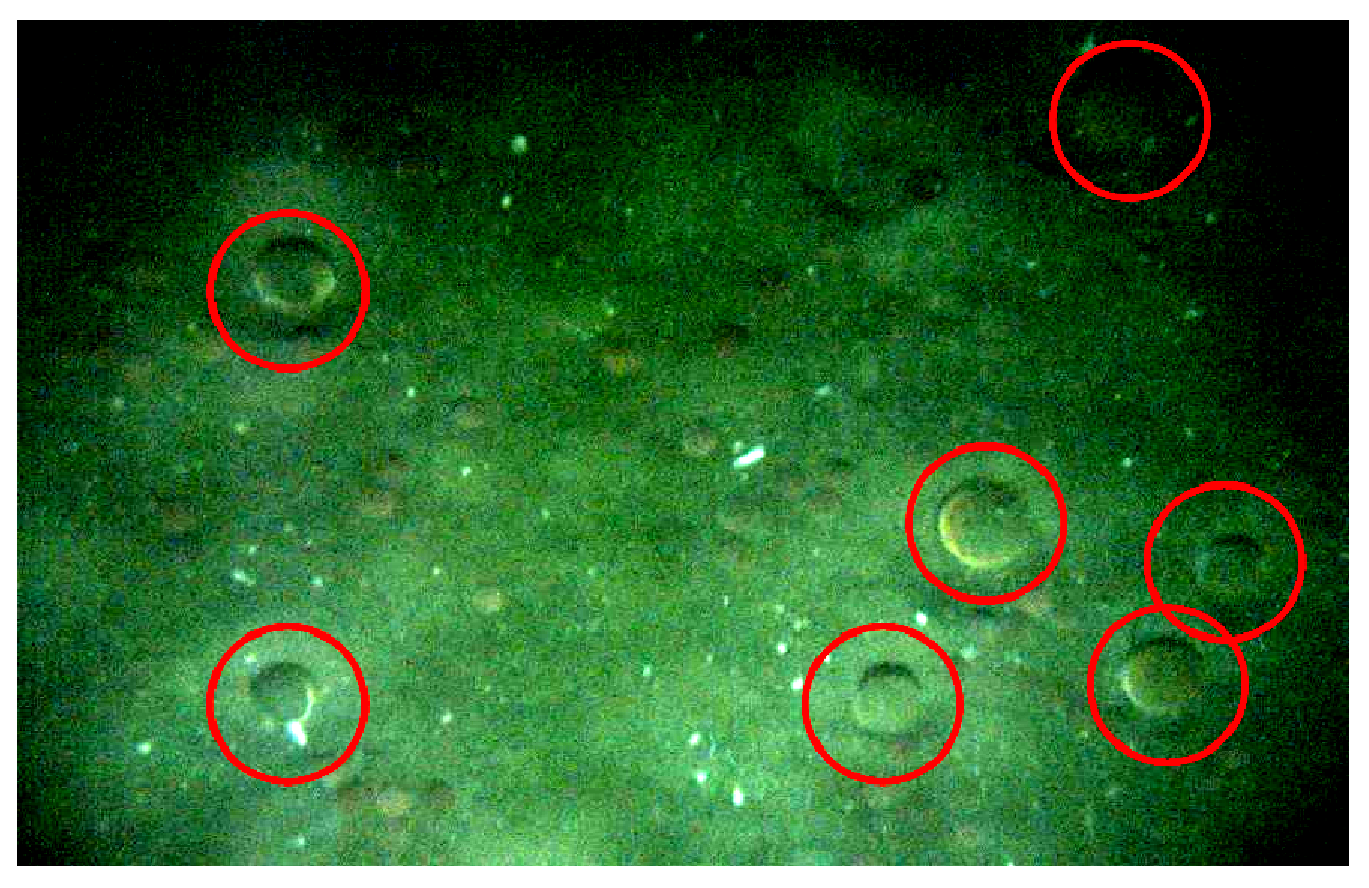
\includegraphics[width=0.6\textwidth]{scallopred}
      \caption[Seabed image with scallops shown in red circles]{Seabed image with scallops shown in red circles}
      \label{fig:scallopred}
\end{figure} 

A visual scallop population assessment process involves identifying these animals in image datasets.
A representative example of an image from the dataset we had to work with is shown in  Figure~\ref{fig:scallopred} (scallops marked within red circles).
A general solution to automated image annotation might not necessarily be effective for the dataset at hand.
The need here is to identify algorithms and methods that will work best under \emph{poor} lighting and imaging conditions, characteristic of this particular scallop counting application. 
The results from using elementary image processing methods like thresholding and edge detection on the images (see Figure~\ref{subfig:thresh_scallop} and \ref{subfig:edge_scallop}) demonstrate the need for a more sophisticated approach (possibly a hybrid combination of several techniques).

\begin{figure}
  \centering
  \begin{subfigure}[]{0.15\textwidth}
      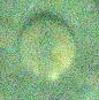
\includegraphics[width=\textwidth]{dcrescent_scallop}
      \caption{}
      \label{subfig:dcrescent_scallop}
  \end{subfigure}
  \begin{subfigure}[]{0.15\textwidth}
      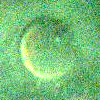
\includegraphics[width=\textwidth]{bcrescent_scallop}
      \caption{}
      \label{subfig:bcrescent_scallop}
  \end{subfigure}
  \begin{subfigure}[]{0.17\textwidth}
      \raisebox{-2pt}{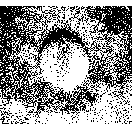
\includegraphics[width=\textwidth]{thresh}}
      \caption{}
      \label{subfig:thresh_scallop}
  \end{subfigure}
  \begin{subfigure}[]{0.17\textwidth}
      \raisebox{-2pt}{
\includegraphics[width=\textwidth]{edge}}
      \caption{}
      \label{subfig:edge_scallop}
  \end{subfigure}
\caption[Scallop features]{(\subref{subfig:dcrescent_scallop}) Scallop with yellowish tinge and dark crescent; (\subref{subfig:bcrescent_scallop}) Scallop with yellowish tinge and bright shell rim crescent; (\subref{subfig:thresh_scallop}) Scallop sample after thresholding; (\subref{subfig:edge_scallop}) Scallop sample after edge detection.
}
\end{figure}

Another challenge, related to the issue of low image resolution and high levels of speckle noise, is the selection of appropriate scallop features that would enable distinguishing between these organisms and other objects. 
In the particular dataset, one recurrent visual pattern is a dark crescent on the upper perimeter of the scallop shell, which is the shadow cast by the upper open scallop shell produced from the \gls{auv} strobe light (see Figure~\ref{subfig:dcrescent_scallop}). 
Another pattern that could serve as a feature in this dataset is a bright crescent on the periphery of the scallop, generally associated with the visible interior of the bottom half when the scallop shell is partly open (see Figure~\ref{subfig:bcrescent_scallop}).
A third pattern may be a yellowish tinge associated with the composition of the scallop image (see Figure~\ref{subfig:bcrescent_scallop}).

We have leveraged visual patterns \cite{prasanna_aslo} to develop a three-layered scallop counting framework  that combines tools from computer vision and machine learning. 
This particular hybrid architecture uses top-down visual attention, graph-cut segmentation and template matching along with a range of other filtering and image processing techniques. 
Though this architecture offers a performance of over 63\% true positive detection rate, it has a very large number of false positives. 
To mitigate this problem, we extend the framework \cite{prasanna_aslo} by adding a fourth, false-positives filtering layer \cite{prasanna_igi}.

%========================================================================================
\section{Scallop Survey Procedure}

The 2011 \gls{rsa} 
project (Titled: ``A Demonstration Sea Scallop Survey of the 
Federal Inshore Areas of the New York Bight using a Camera Mounted Autonomous Underwater
 Vehicle'')
was a proof-of-concept project that successfully used a digital, rapid-fire camera integrated 
to a Gavia \gls{auv}, to collect a continuous record of photographs for mosaicking, 
and subsequent scallop enumeration. 
In July 2011, transects were completed in the northwestern waters of the mid-Atlantic 
Bight at depths of 25-50 m.  The \gls{auv} continuously photographed the 
seafloor along each transect at a constant distance of 2\,m above the seafloor.  
Parallel sets of transects were spaced as close as 4\,m.  
Georeferenced images were manually analyzed for the presence of sea scallops 
using position data logged (using \gls{dvl} and \gls{ins}) with each image.
%
\subsection{Field Survey Process}
%
\begin{figure}
\centering
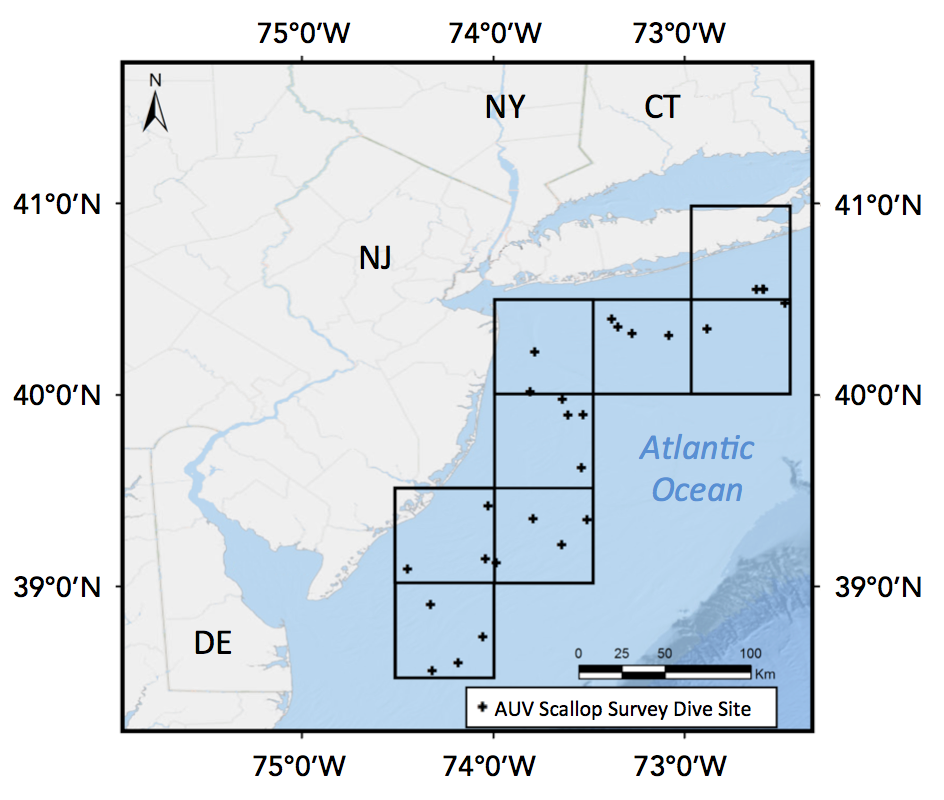
\includegraphics[width=0.5\textwidth, natwidth=944, natheight=800]{survey_region}
\caption[Map of the scallop survey region]{Map of the survey region from Shinnecock, New York to Cape May, New Jersey, 
divided into eight blocks or strata}
\label{fig:strata}
\end{figure}
%

In the 2011 demonstration survey, the federal inshore scallop grounds from Shinnecock, New York to Ocean View, Delaware, was divided into eight blocks or strata (as shown in Figure~\ref{fig:strata}).  
The \textit{f/v Christian and Alexa} served as the surface support platform 
from which a Gavia \gls{auv} (see Figure~\ref{fig:gavia_auv}) was deployed and recovered.  The \gls{auv} 
conducted photographic surveys of the seabed for a continuous duration of approximately
3 hours during each dive, repeated 3--4 times in each stratum, with
each stratum involving roughly 10 hours of imaging and an area of about $45\,000$ 
m$^2$.
The \gls{auv} collected altitude (height above the seabed) and 
attitude (heading, pitch, roll) data, allowing the georectification of each image 
into scaled images for size and counting measurements.  During the 2011 pilot study 
survey season, over $250\,000$ images of the seabed were collected. 
These images were analyzed in the University of Delaware's Coastal Sediments, Hydrodynamics and Engineering 
Laboratory for estimates of scallop
abundance and size distribution.  The \textit{f/v Christian and Alexa} provided 
surface support, and made tows along the \gls{auv} transect to ground-truth the presence of 
scallops and provide calibration for the size distribution. 
Abundance and sizing estimates were computed manually for each image using a GUI-based 
digital sizing software. 
Each image included embedded metadata that 
allowed it to be incorporated into existing benthic image classification systems
(HabCam mip \cite{dawkings13}).
% Abundance and sizing estimates were conducted via a heads-up manual method, 
% with each image including embedded metadata allowing it to be incorporated into 
% to existing benthic image classification systems (HabCam mip \citep{Dawkings13}).

During this proof of concept study, in each stratum the f/v
\textit{Christian and Alexa} made one 15-minute dredge tow along the \gls{auv} 
transect to ground-truth the presence of scallops and other fauna, 
and provide calibration for the size distribution.  The vessel was maintained 
on the dredge track by using Differential GPS.  
The tows were made with the starboard 15 ft 
(4.572\;m)
wide New Bedford style commercial dredge at the commercial dredge speed of 4.5--5.0 knots.
The dredge was equipped with 4 inch (10.16 m) interlocking rings, 
an 11 inch (27.94 cm) twine mesh top, and turtle chains.
After dredging, the catch was sorted, identified, and weighed.  
Length-frequency data were obtained for the caught scallops.  
This information was recorded onto data logs and then entered into a laptop computer database aboard ship for comparison to the camera image estimates.

The mobile platform of the \gls{auv} provided a more expansive and continuous coverage 
of the seabed compared to traditional fixed drop camera systems or towed camera systems. 
In a given day, the \gls{auv} surveys covered about $60\,000$\;m$^2$ of seabed 
from an altitude of 2\;m above the bed, simultaneously producing broad sonar 
swath coverage and measuring the salinity, temperature, dissolved oxygen, and 
chlorophyll-a  in the water.


\subsection{Sensors and Hardware}
\label{section:equipment}

The University of Delaware \gls{auv} (Figure \ref{fig:gavia_auv}) was used to collect 
continuous images of the benthos, and simultaneously map the texture and topography of 
the seabed. Sensor systems associated with this vehicle include: \begin{enumerate*}[label=(\arabic*):, start=1] 
\item a 500\;kHz GeoAcoustics GeoSwath Plus phase measuring bathymetric 
sonar; \item a 900/1800\;kHz Marine Sonic dual-frequency high-resolution 
side-scan sonar; 
\item a Teledyne Rd Instruments 1200 kHz acoustic \gls{dvl}/\gls{adcp}; 
\item a Kearfott T-24 inertial navigation system; 
\item an Ecopuck flntu combination fluorometer / turbidity sensor; 
\item a Point Grey Scorpion model 20SO digital camera and LED strobe array; 
\item an Aanderaa Optode dissolved oxygen sensor; 
\item a temperature and density sensor; and, \item an altimeter. \end{enumerate*} 
Each sensor separately records time and spatially stamped data with frequency and spacing.
The \gls{auv} is capable of very precise dynamic positioning, adjusting to the variable 
topography of the seabed while maintaining a constant commanded altitude offset.

\begin{figure}
  \centering
  \begin{subfigure}[]{0.7\textwidth}
      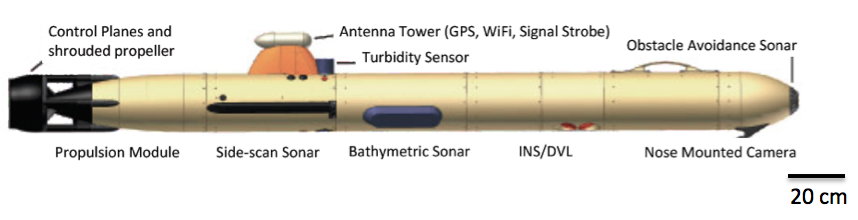
\includegraphics[width=\textwidth,natwidth=1052,natheight=428]{auv_schematics}
  \end{subfigure}
  \begin{subfigure}[]{0.6\textwidth}
      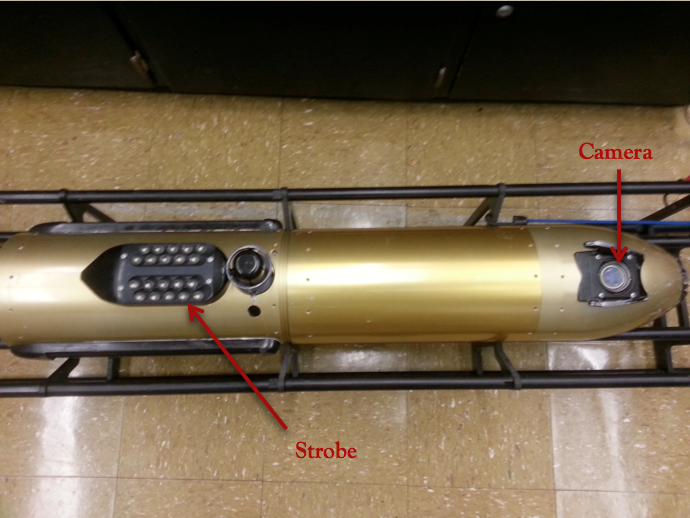
\includegraphics[width=\textwidth,natwidth=690,natheight=518]{auv_image}    
  \end{subfigure}
  \caption{Schematics and image of the Gavia \gls{auv} }
  \label{fig:gavia_auv}
\end{figure}

\subsection{Data Collection}

The data was collected over two separate five-day cruises in July 2011.   
In total, 27 missions were run using the \gls{auv} to photograph the seafloor (For list of missions see Table \ref{tab:mission_list}).  
Mission lengths were constrained by the 2.5 to 3.5 hour battery life of the \gls{auv}.  
During each mission, the \gls{auv} was instructed to follow a constant height of 2\;m
above the seafloor.  In addition to the $250\,000$ images that were collected, the 
\gls{auv} also gathered data about water temperature, salinity, dissolved oxygen, 
geoswath bathymetry, and side-scan sonar of the seafloor.

The camera on the \gls{auv}, a Point Grey Scorpion model 20SO (for camera specifications see Table \ref{tab:camera_specs}), 
was mounted inside the nose module of the vehicle.
It was focused at 2\;m, and captured
images at a resolution of $800\times600$.  The camera lens had a horizontal viewing 
angle of 44.65 degrees.  Given the viewing angle and distance from the seafloor, 
the image footprint can be calculated as $1.86\times1.40$\;m$^2$.
Each image was saved in jpeg format, with metadata that included position information 
(including latitude, longitude, depth, altitude, pitch, heading and roll)  
and the near-seafloor environmental conditions analyzed in this study.  
This information is stored in the header file, making the images readily comparable and 
able to be incorporated into existing \gls{rsa} image databases, such as the 
HabCam database.
A manual count of the number of scallops in each image was performed and used to obtain overall scallop
abundance assessment.
Scallops counted were articulated shells in life position (left valve up) \cite{walker}.
%
\begin{table}
\centering
\begin{threeparttable}
      \begin{tabular}{ll}
      \toprule[1pt]\\[-6pt]
      Mission  & Number of images\\[2pt]\midrule
      LI1\tnote{1}	&$12\,775$\\
      LI2	&$2\,387$\\
      LI3	&$8\,065$\\
      LI4	&$9\,992$\\
      LI5	&$8\,338$\\
      LI6	&$11\,329$\\
      LI7	&$10\,163$\\
      LI8	&$9\,780$\\
      LI9	&$2\,686$\\
      NYB1\tnote{2}	&$9\,141$\\
      NYB2	&$9\,523$\\
      NYB3	&$9\,544$\\
      NYB4	&$9\,074$\\
      NYB5	&$9\,425$\\
      NYB6	&$9\,281$\\
      NYB7	&$12\,068$\\
      NYB8	&$9\,527$\\
      NYB9	&$10\,950$\\
      NYB10	&$9\,170$\\
      NYB11	&$10\,391$\\
      NYB12	&$7\,345$\\
      NYB13	&$6\,285$\\
      NYB14	&$9\,437$\\
      NYB15	&$11\,097$\\
      ET1\tnote{3}	&$9\,255$\\
      ET2	&$12\,035$\\
      ET3	&$10\,474$\\
      \\[2pt]\bottomrule[1pt]
    \end{tabular}
    \begin{tablenotes}
       \vskip 5pt
	  \item[1] \footnotesize{LI--Long Island}
	  \item[2] \footnotesize{NYB--New York Bight}
	  \item[3] \footnotesize{ET--Elephant Trunk}
      \end{tablenotes}                                                      
 \end{threeparttable}
  \caption{List of missions and number of images collected}
  \label{tab:mission_list}
\end{table}

%                                                      
\begin{table}                                                     
\centering
\begin{tabularx}{\textwidth}{XX}
\toprule[1pt]\\[-6pt]
Attribute	&Specs\\[2pt]\midrule
Name	&Point Grey Scorpion 20SO Low Light Research Camera\\
Image Sensor	&8.923 mm Sony ccd\\
Horizontal Viewing Angle	&44.65 degrees (underwater)\\
Mass	&125 g\\
Frame rate	&3.75 fps\\
Memory	&Computer housed in \gls{auv} nose cone\\
Image Resolution	&800 $\times$ 600\\
Georeferenced metadata	&Latitude, longitude, altitude, depth\\
Image Format	&jpeg\\[2pt]\bottomrule[1pt]
\end{tabularx}
\caption{Camera specifications\label{tab:camera_specs}}
\end{table}


%========================================================================================
\section{Methodology}

The multi-layered scallop counting framework that comprises four layers of processing on underwater images for the purpose of obtaining scallop counts is discussed in this section. 
The four layers involve the sequential application of Top-Down Visual Attention, Segmentation, Classification and False-Positive Filtering.

\subsection{Layer I: Top-Down Visual Attention} \label{subsec:TDVA}

\subsubsection{Learning}

A customized \gls{tdva} algorithm can be designed 
to sift automatically through the body of imagery data, and focus on
regions of interest that are more likely to contain scallops.
The process of designing the \gls{tdva} algorithm is described below.

The first step is a small-scale, \gls{buva} based saliency computation. 
The saliency computation is performed 
on a collection of randomly selected 243 annotated images, collectively containing 300 scallops.
This collection constitutes the \emph{learning set}.
Figure~\ref{fig:saliency_combine} represents graphically the flow of computation
and shows the type of information in a typical image that visual attention tends to highlight.
%
\begin{figure*}
\vskip -5pt
\centering
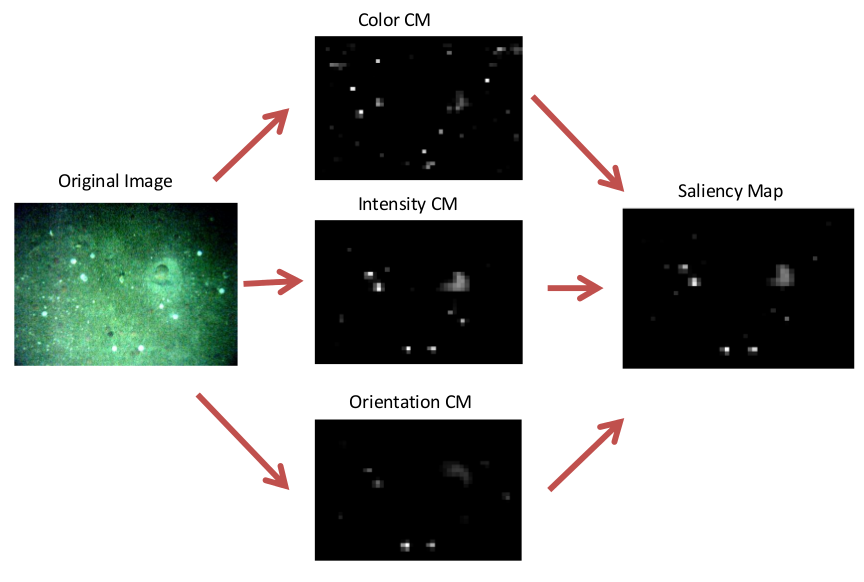
\includegraphics[width=0.80\textwidth,natwidth=864,natheight=582]{saliency_example1.png}
\caption{Illustration of computation flow for the construction of saliency maps}
\label{fig:saliency_combine}
\end{figure*}
%

A process of extremum
seeking on the saliency map of each image identifies fixations in the associated image.
If a $100\times100$ pixel window---corresponding to an approximately $23 \times 23$\enspace cm$^2$ area on the seafloor---centered around a fixation point
contained the center of a scallop, the corresponding 
fixation was labeled a \emph{target}; otherwise, it is considered a \emph{distractor}.

\begin{figure} 
% \vskip +6pt
\centering
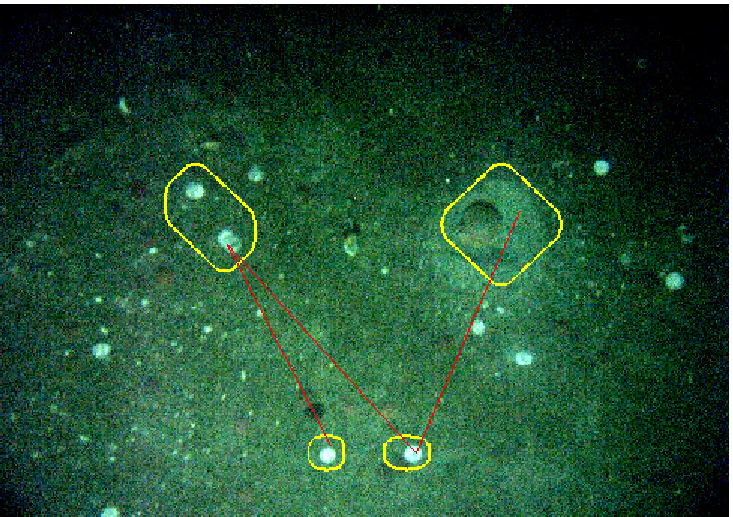
\includegraphics[width=0.6\textwidth,natwidth=800,natheight=600]{fixation_example.pdf}
\caption[Illustration of fixations]{Illustration of fixations (marked by yellow boundaries):
         red lines indicate the order in which the fixations were detected with the lower-left fixation being the first.
}
\label{fig:fixation}
%\vskip -15pt
\end{figure}

The target and distractor regions are determined in all the feature and conspicuity maps for each one of these processed images in the learning set.
This is done by adaptively thresholding and locally segmenting the points around the fixations with similar salience values in each map.
Then the mean numerical value in neighborhoods around  
these target and distractor regions in the feature maps and conspicuity maps 
are computed.  These values are used to populate the $P_{ijT_k}$ and $P_{ijD_r}$ variables in \eqref{eq:learning_wts_all}, and determine the top-down weights for feature maps and conspicuity maps.

For the conspicuity maps, the center-surround scale weights $w_{cs}$ computed through \eqref{eq:learning_wts_all} and consequently used in \eqref{eq:feature_map},
are shown in Table \ref{tab:tdva_fm_wts}.
For the saliency map computation, the weights resulting from the application of
\eqref{eq:learning_wts_all} on the conspicuity maps are
$w_{\bar{I}}= 1.1644$, $w_{\bar{C}}= 1.4354$ and $w_{\bar{O}}= 0.4001$.  
The symmetry of the scallop shell in our low-resolution dataset 
justifies the relatively small value of the orientation weight.

\begin{table*}
\caption{Top-down weights for feature maps \label{tab:tdva_fm_wts}}
\centering
\begin{tabular}{llllllll}
\toprule[1pt]\\[-6pt]
 &   & \multicolumn{6}{c}{Center Surround Feature Scales}\\[2pt]\cline{1-8}\\[-5pt]
  &   & 1 & 2 & 3 & 4 & 5 & 6\\[2pt]\cline{1-8}\\[-5pt]
Color & red-green & 0.8191 & 0.8031 & 0.9184 & 0.8213 & 0.8696 & 0.7076\\
  & blue-yellow & 1.1312 & 1.1369 & 1.3266 & 1.2030 & 1.2833 & 0.9799\\[8pt]
Intensity & intensity & 0.7485 & 0.8009 & 0.9063 & 1.0765 & 1.3111 & 1.1567\\[8pt]
Orientation & $0^\circ$ & 0.7408 & 0.2448 & 0.2410 & 0.2788 & 0.3767 & 2.6826\\
  & $45^\circ$ & 0.7379 & 0.4046 & 0.4767 & 0.3910 & 0.7125 & 2.2325\\
  & $90^\circ$ & 0.6184 & 0.5957 & 0.5406 & 1.2027 & 2.0312 & 2.1879\\
  & $135^\circ$ & 0.8041 & 0.6036 & 0.7420 & 1.5624 & 1.1956 & 2.3958\\[2pt]\bottomrule[1pt]
\end{tabular}
\end{table*}
% 

                                                   

\subsubsection{Implementation and Testing}\label{sec:tdva-testing}

To test the performance of the customized \gls{tdva} algorithm, it is applied on
two image datasets, the size of which is shown in Table~\ref{tab:count_results}.
In this application, the saliency maps are computed via the formulae 
\eqref{eq:saliency_map} and \eqref{eq:feature_map},
using the weights listed in Table \ref{tab:tdva_fm_wts}.
Convergence time of the winner-takes-all neural network that finds fixations in the saliency map of each image in the datasets of Table~\ref{tab:count_results}, is controlled using dynamic thresholding:
It is highly unlikely that a fixation that contains an object of interest
requires more than $10\,000$ iterations. If convergence to some fixation takes 
more than this number of iterations, 
then the search is terminated and no more fixations
are sought in the image.

Given that an image in datasets of
Table~\ref{tab:count_results} contains two scallops on average, no more than
ten fixations are sought in each image (The percentage of images
in the datasets that contained more than $10$ scallops 
was $0.002\%$).
Since in the testing phase the whole scallop---not just the center---needs to be included in the fixation window, the size of this window is set at
$270\times270$ pixels; more than $91$\% of the scallops are accommodated inside the window (Figure~\ref{fig:window_length}). 

\begin{figure}
  \centering
  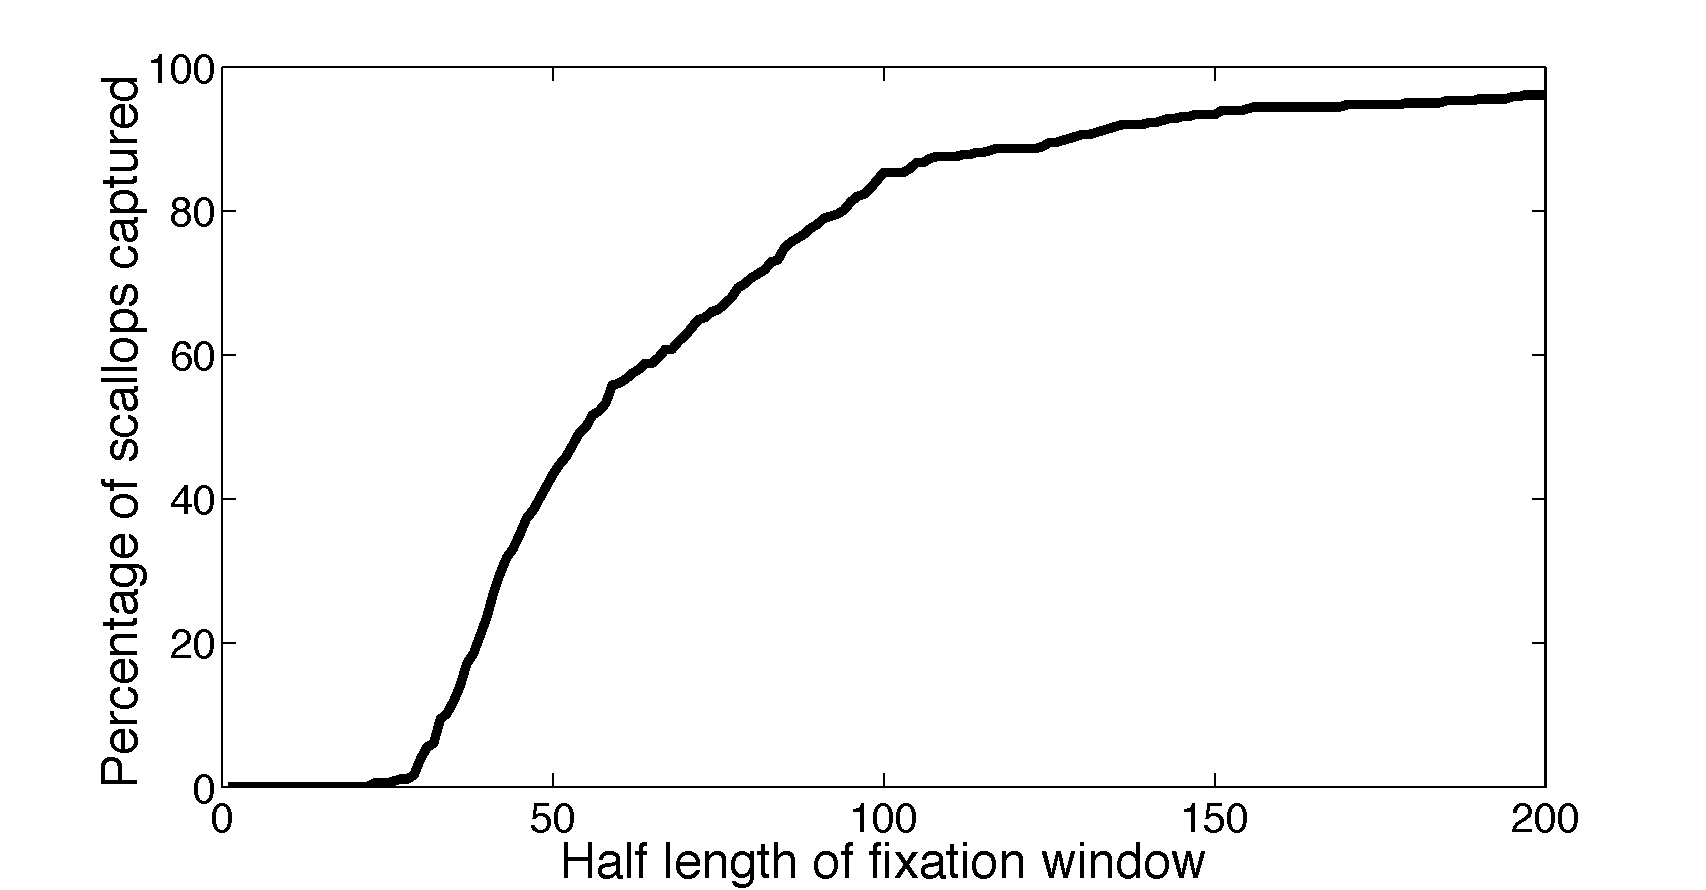
\includegraphics[width=0.60\textwidth,natwidth=800,natheight=600]{windowlength.pdf}
  \caption[Scallop fixation window dimension analysis]{Percentage of scallops enclosed in the fixation window as a function of
  window half length (in pixels)}
  \label{fig:window_length}
\end{figure}

\begin{figure*}
  \centering
  \begin{subfigure}[]{0.17\textwidth}
      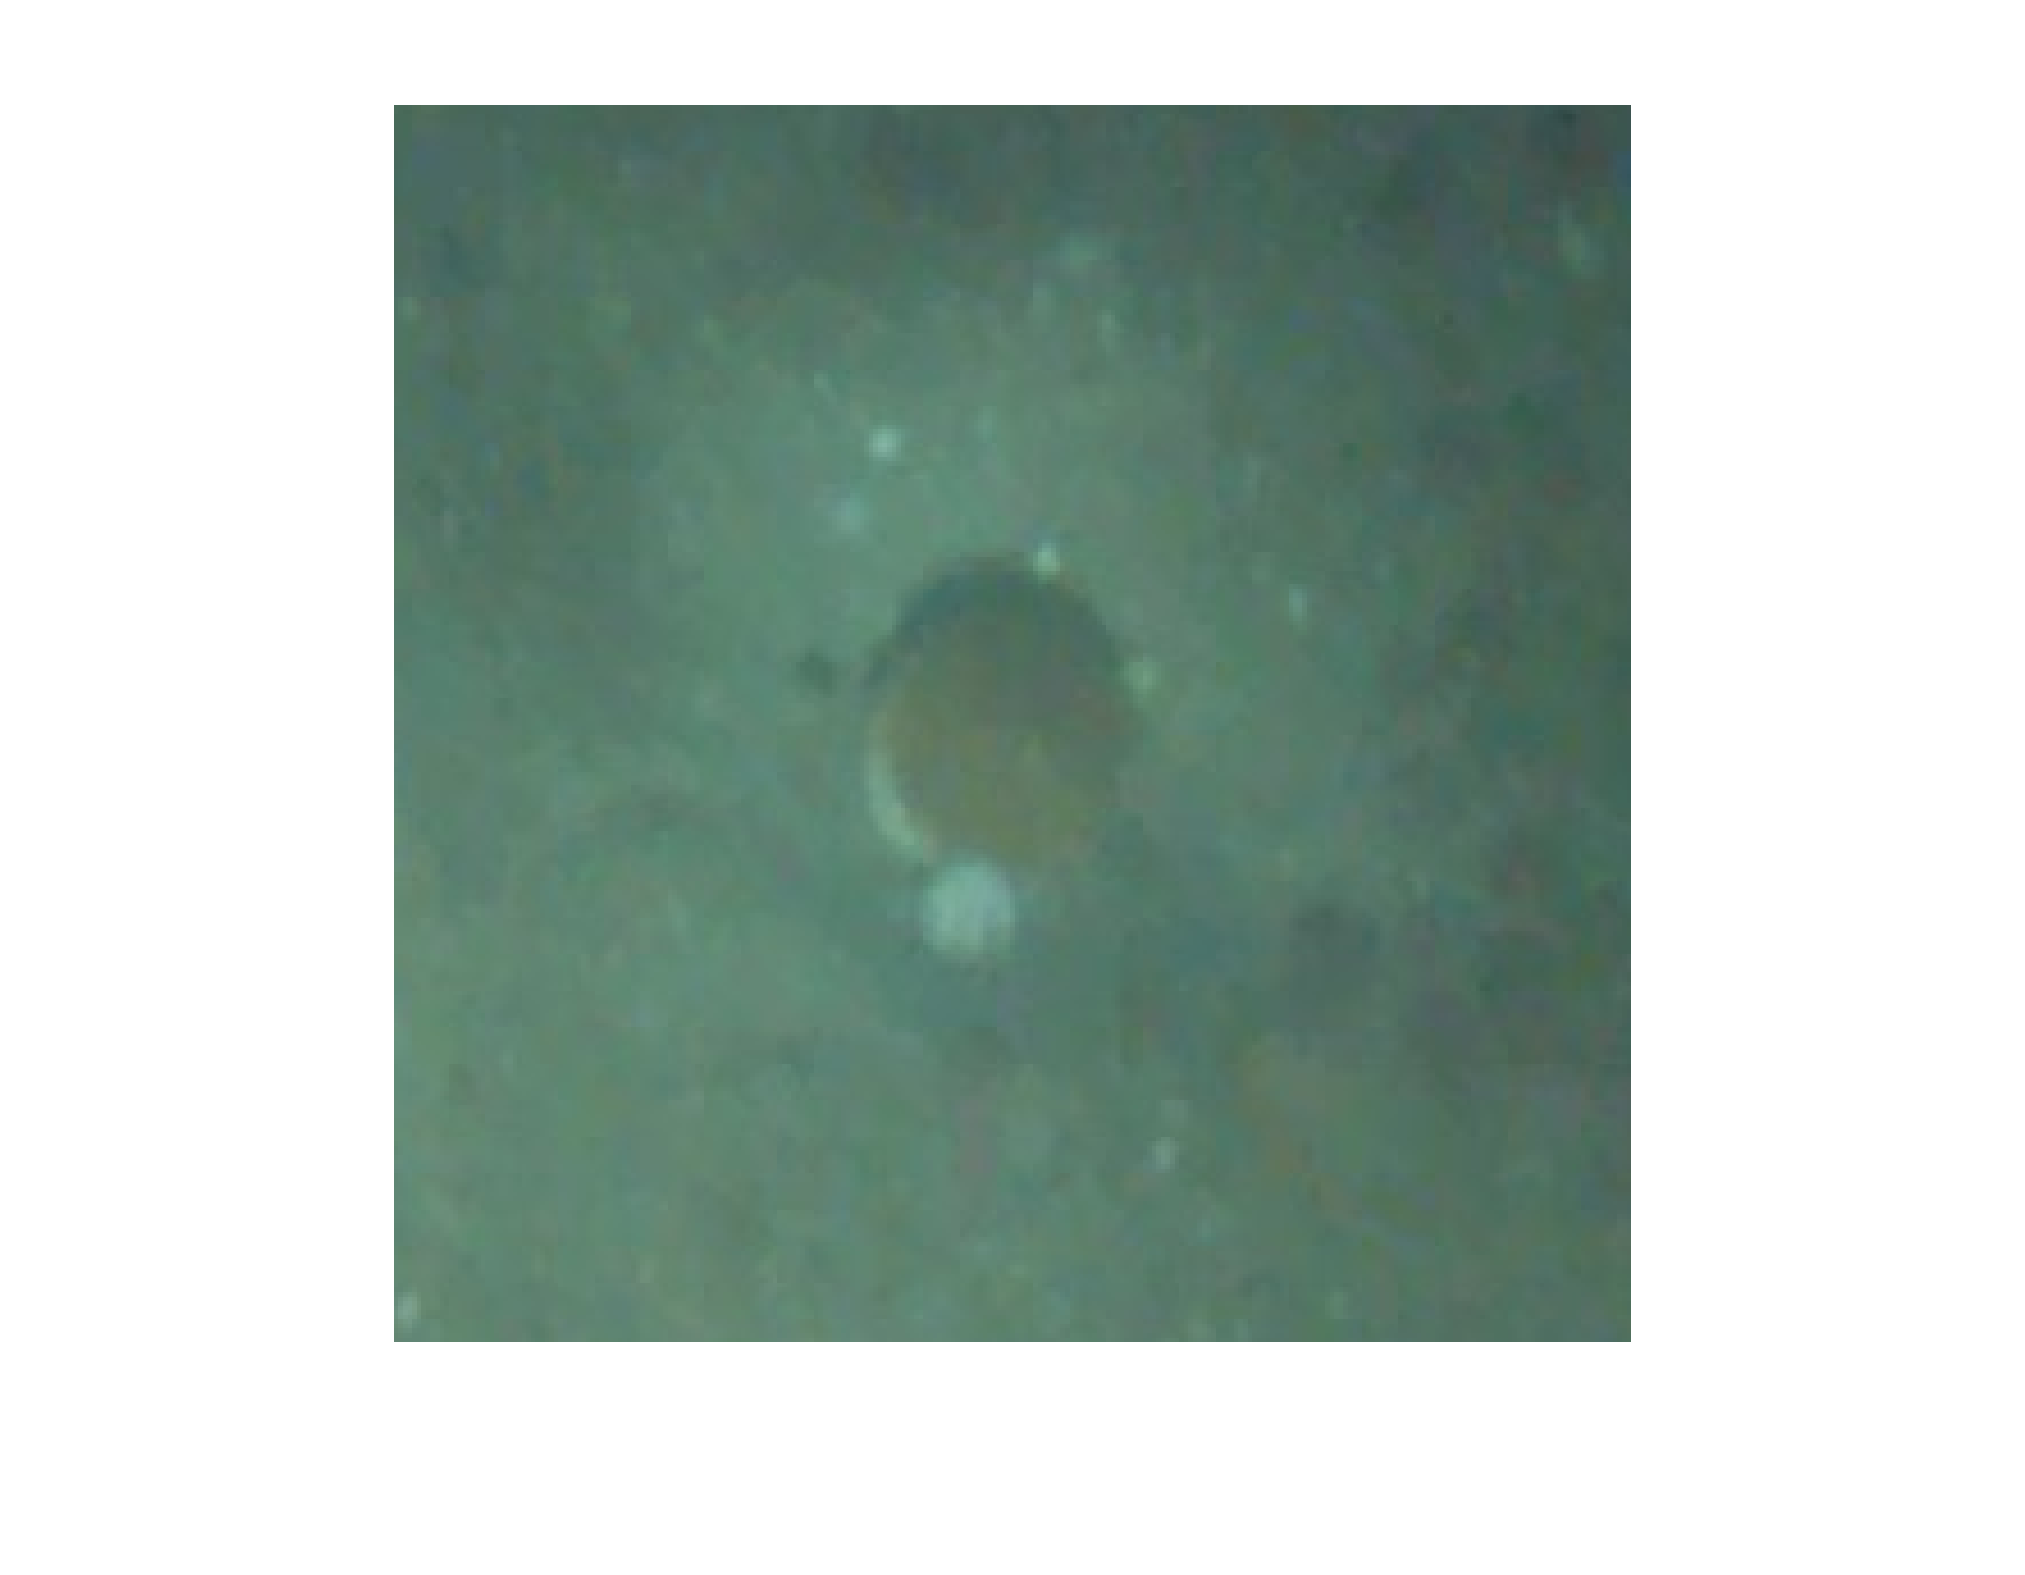
\includegraphics[width=\textwidth,natwidth=842,natheight=844]{fixationwindow.pdf}
      \caption{}
      \label{subfig:fixationwindow}
  \end{subfigure}
  \begin{subfigure}[]{0.17\textwidth}
      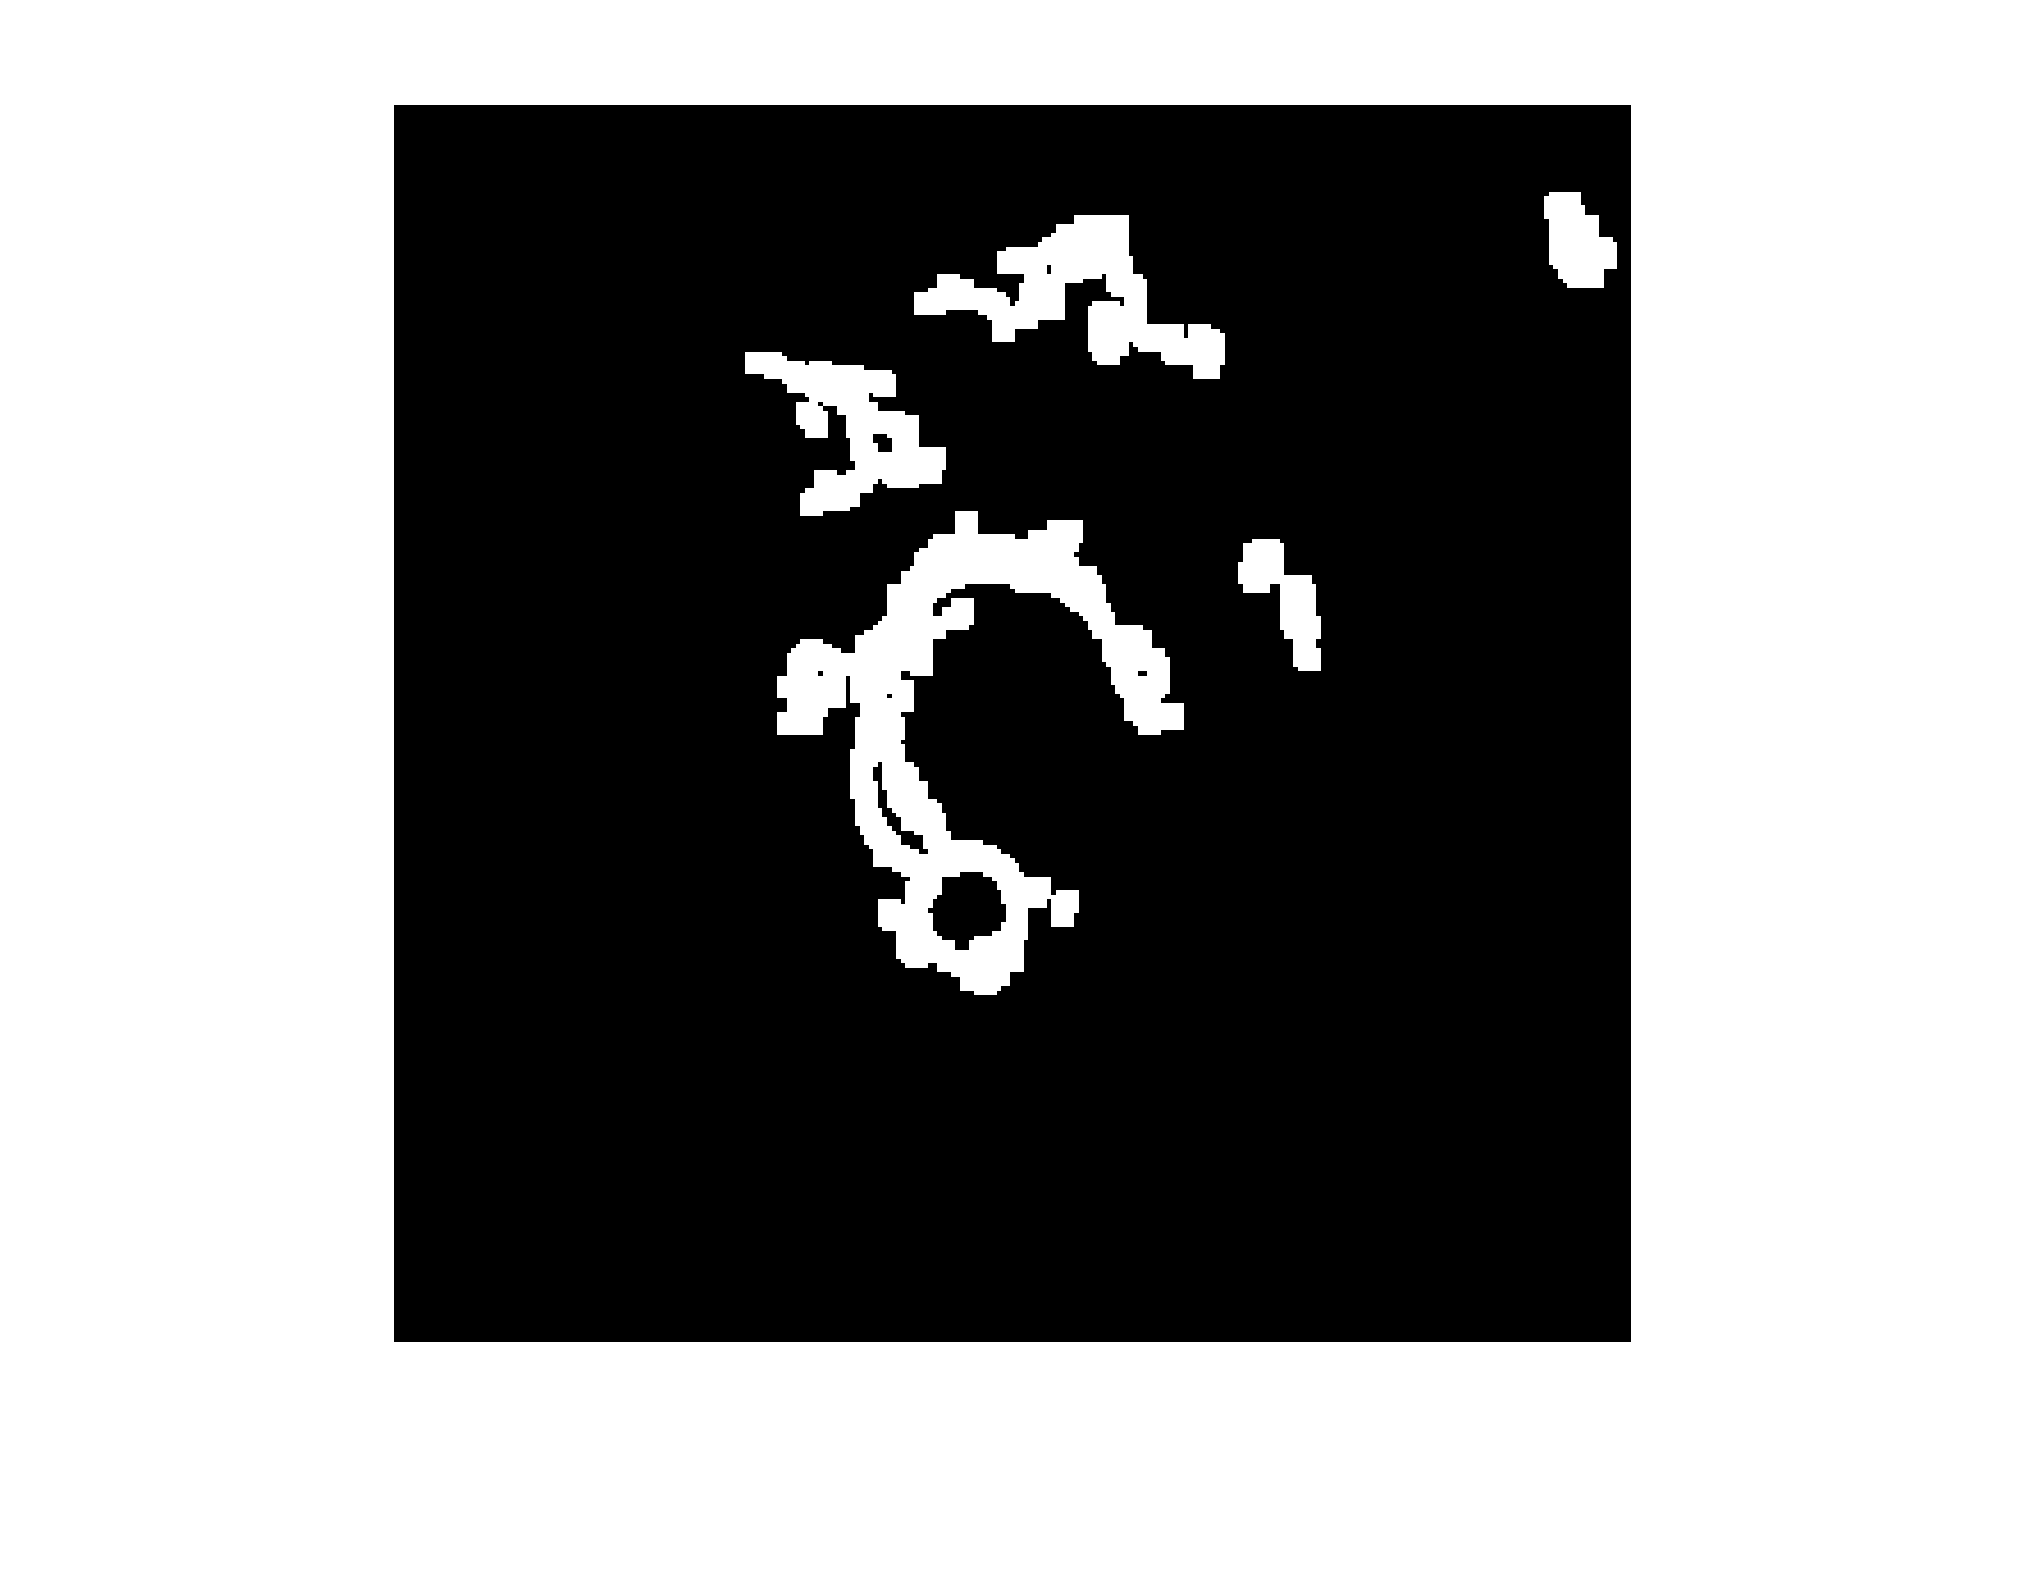
\includegraphics[width=\textwidth,natwidth=837,natheight=839]{edgeimg.pdf}
      \caption{}
      \label{subfig:edgeimg}
  \end{subfigure}
  \begin{subfigure}[]{0.17\textwidth}
      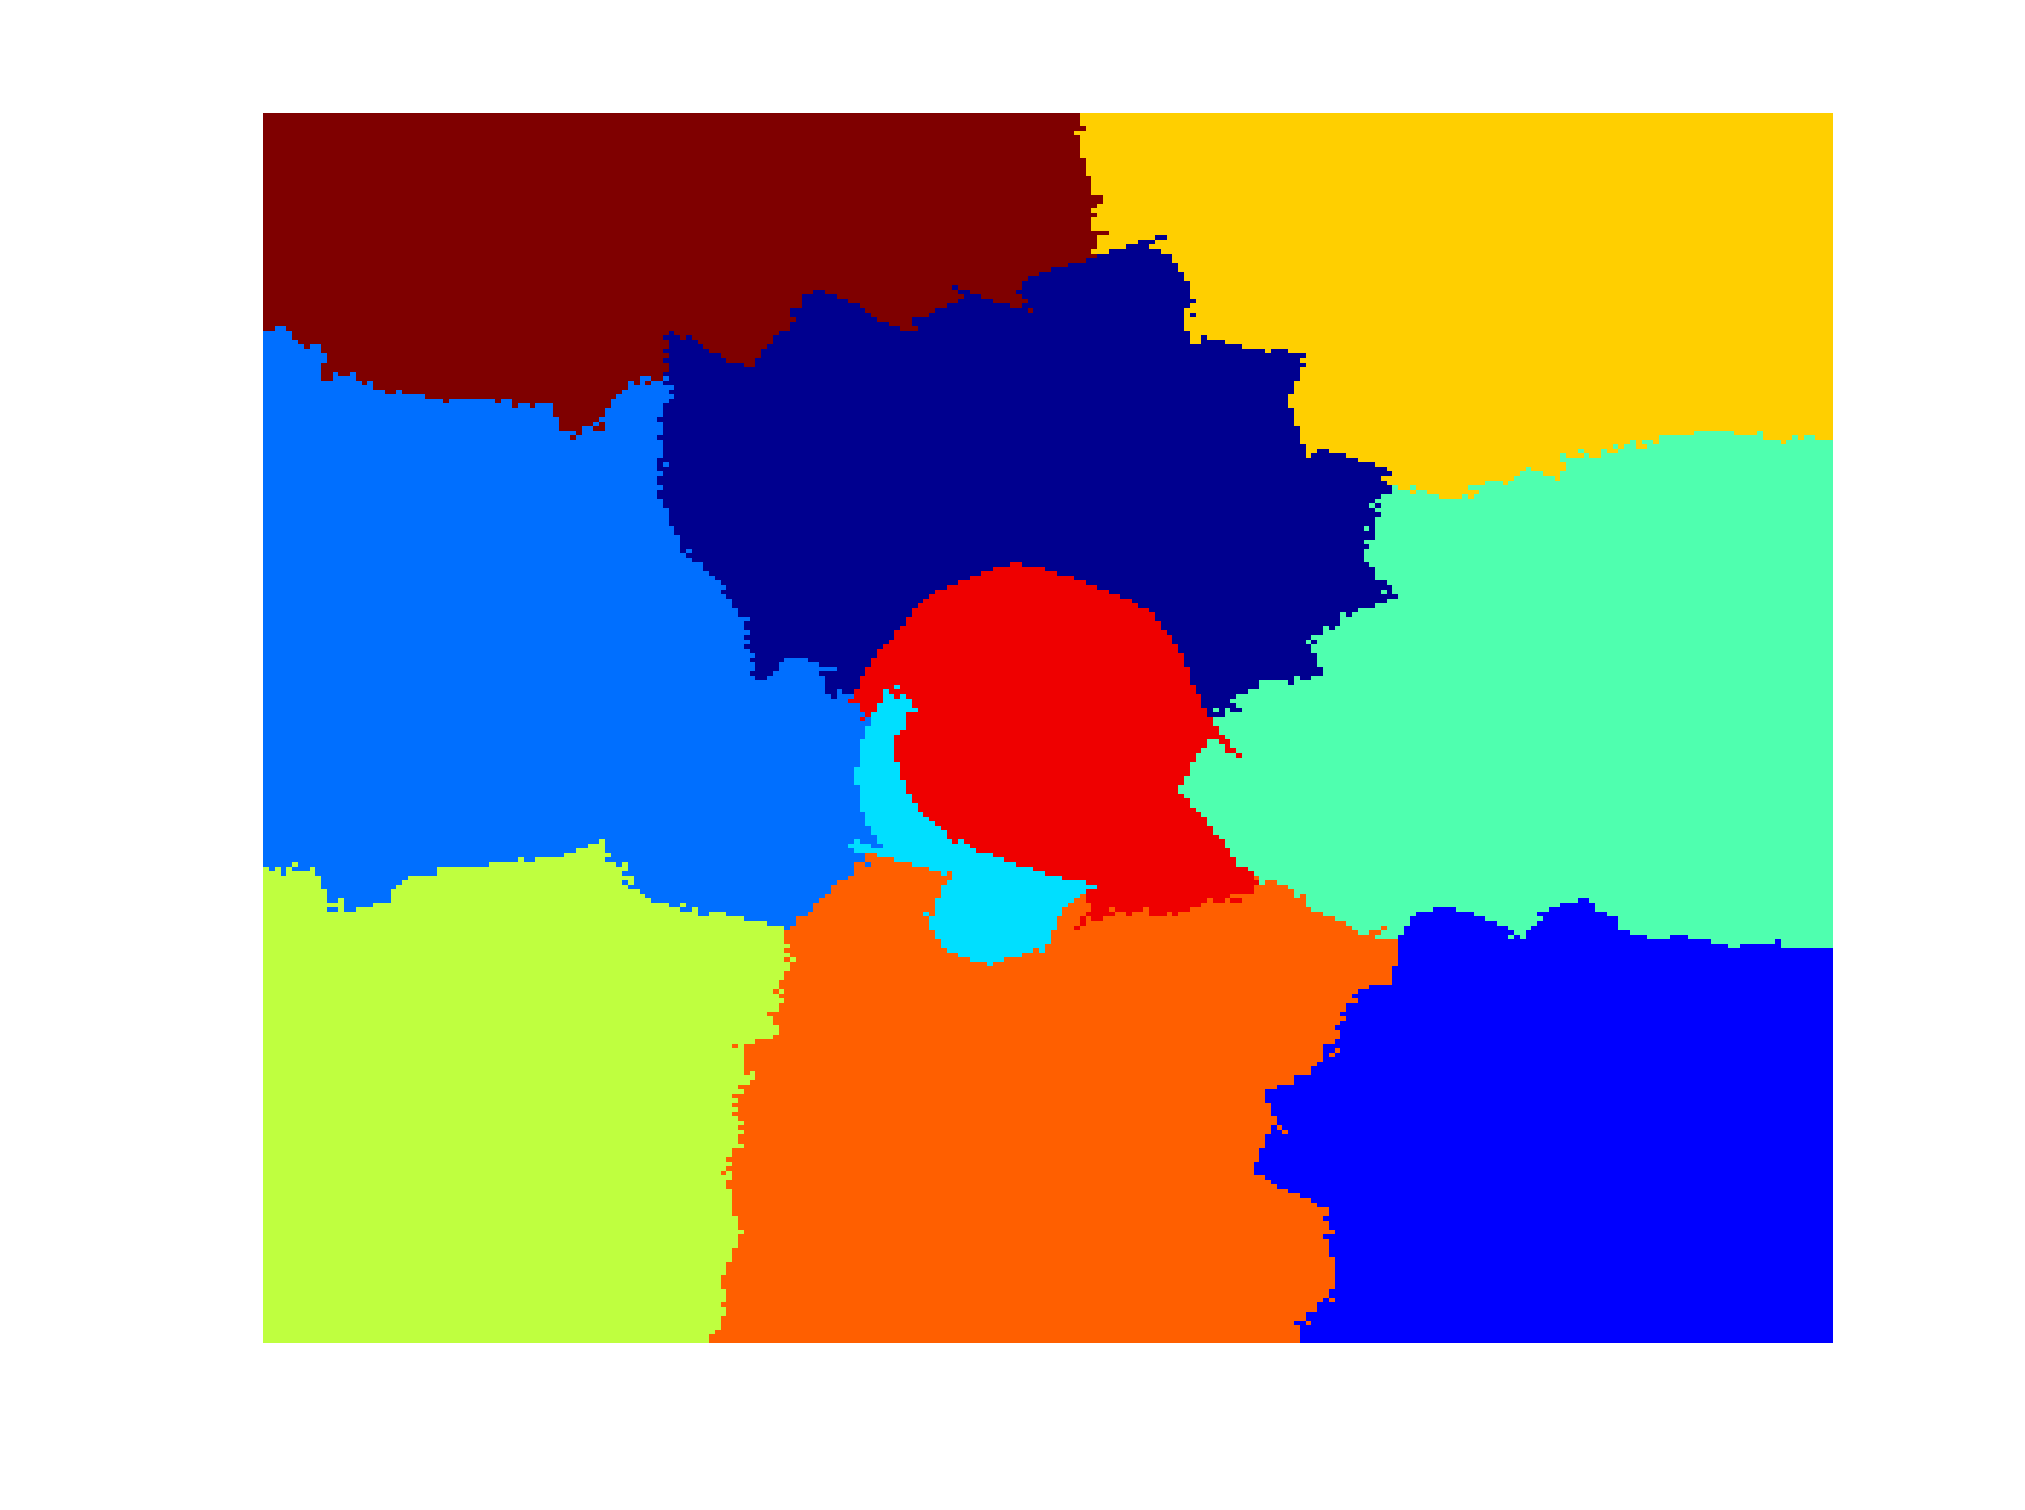
\includegraphics[width=\textwidth,natwidth=1055,natheight=842]{graphimg.pdf}    
      \caption{}
      \label{subfig:graphimg}
  \end{subfigure}
  \begin{subfigure}[]{0.17\textwidth}
      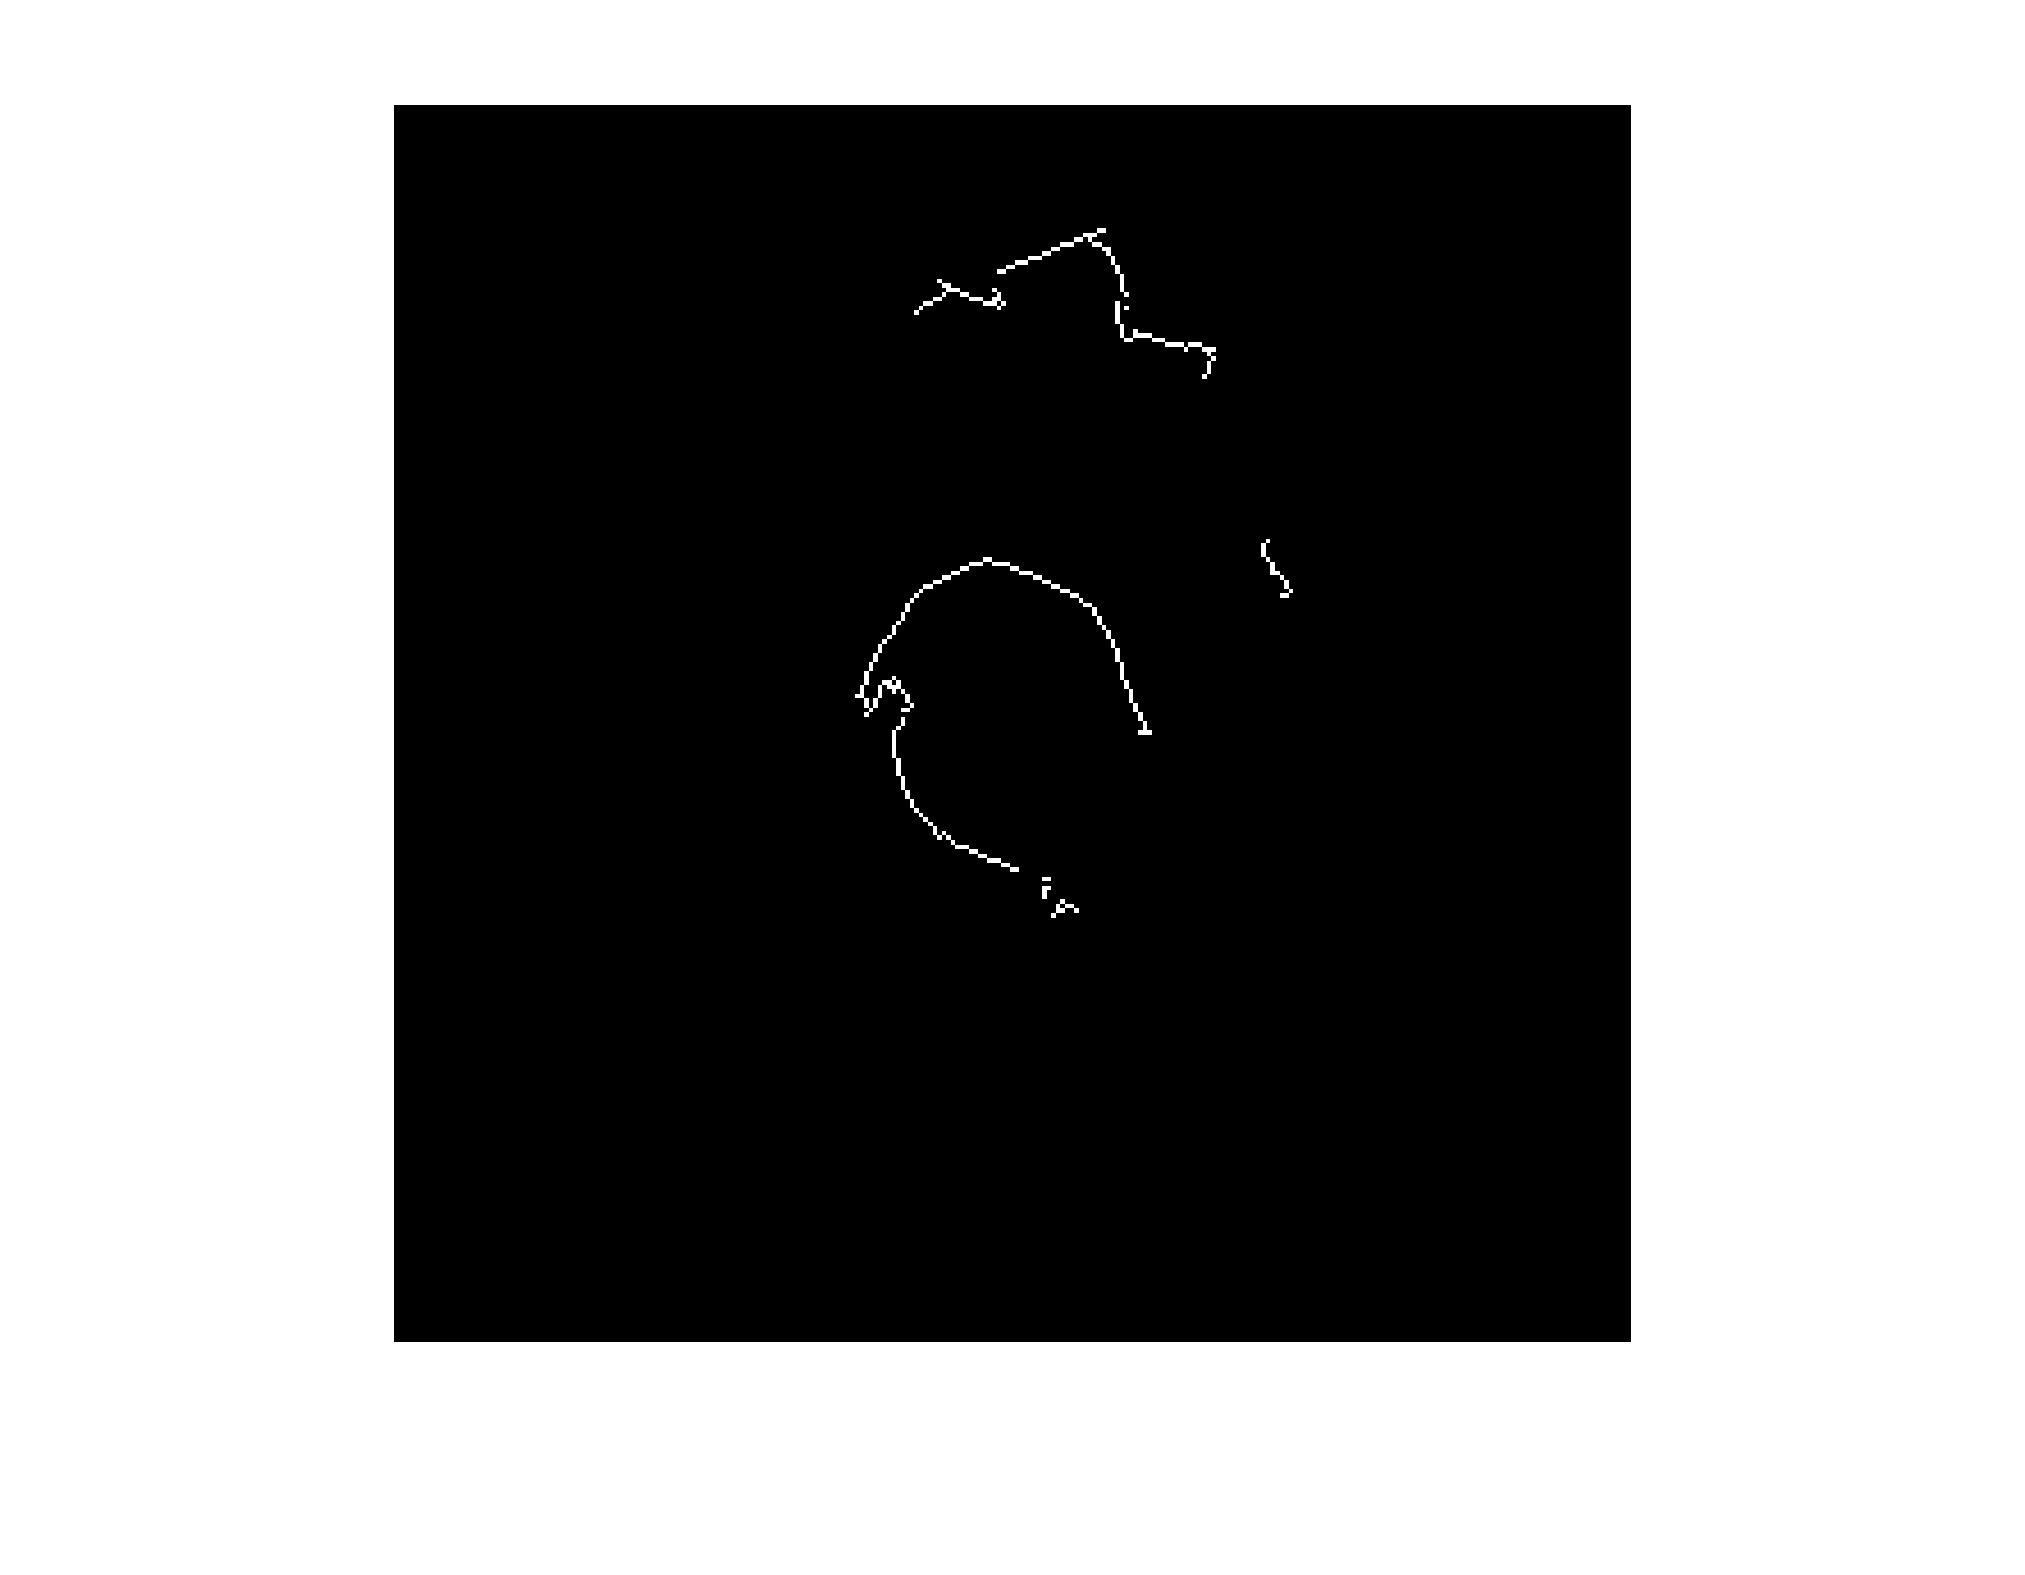
\includegraphics[width=\textwidth,natwidth=834,natheight=837]{regboundry.pdf}
      \caption{}
      \label{subfig:regboundry}
  \end{subfigure}
  \begin{subfigure}[]{0.17\textwidth}
      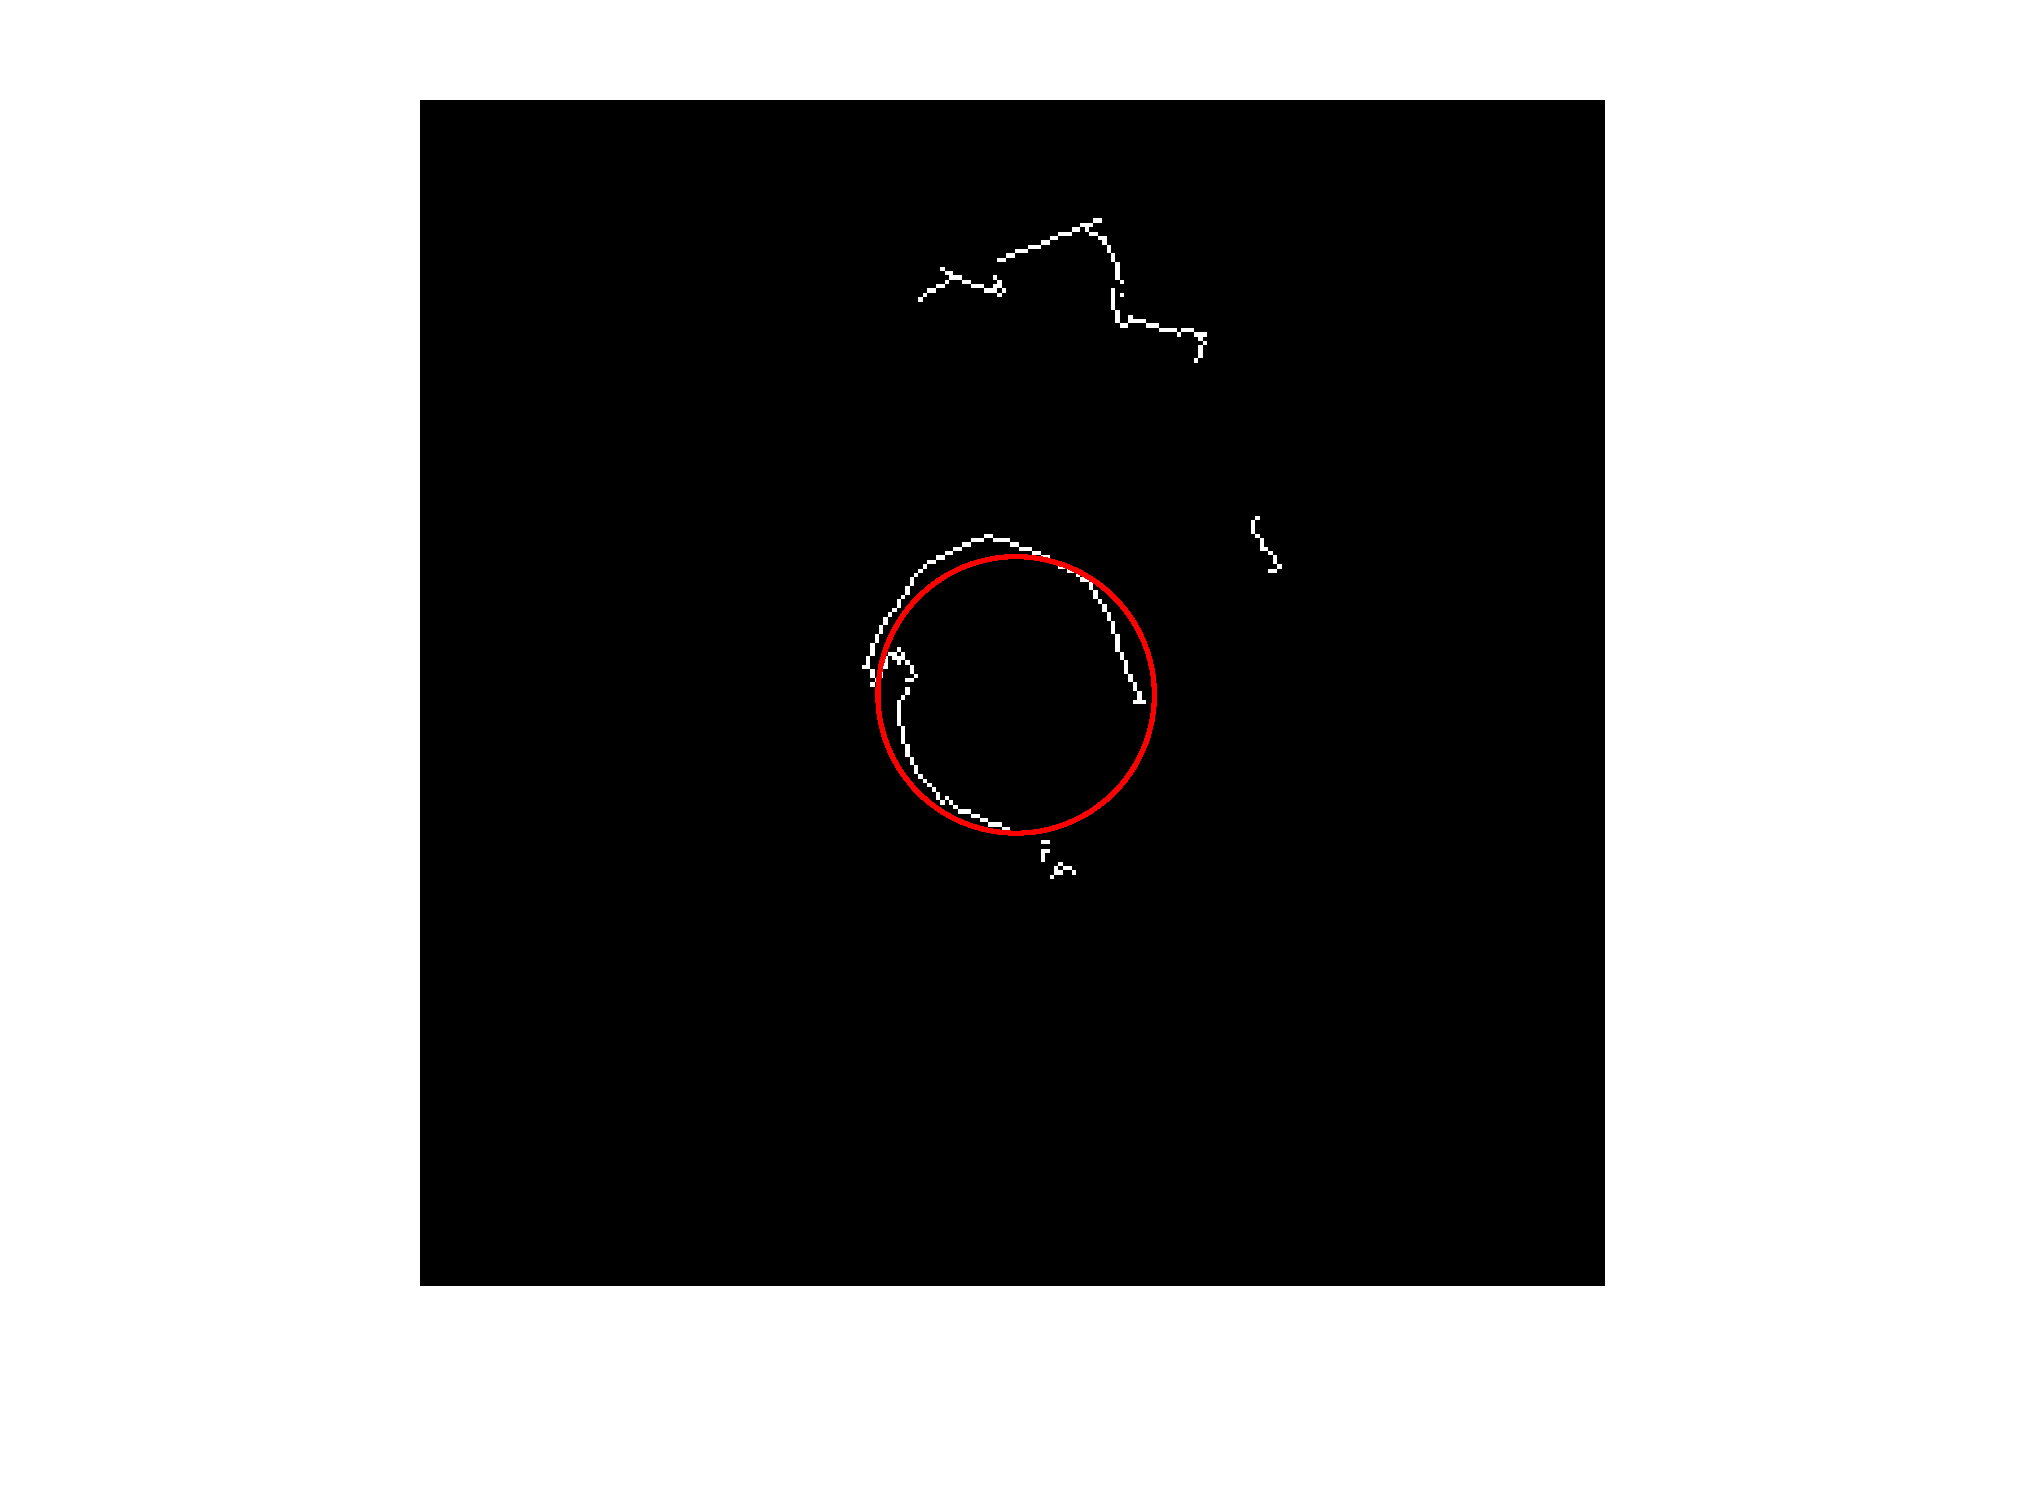
\includegraphics[width=\textwidth,natwidth=810,natheight=813]{regcircle.pdf}         
      \caption{}
      \label{subfig:regcircle}
  \end{subfigure}
\caption[Segmentation layer process flow]{(\subref{subfig:fixationwindow}) Fixation window from layer I; (\subref{subfig:edgeimg}) Edge segmented image; (\subref{subfig:graphimg}) graph-cut segmented image; (\subref{subfig:regboundry}) Region boundaries obtained when the edge segmented image is used as a mask over the graph-cut segmented image boundaries; (\subref{subfig:regcircle}) circle fitted on the extracted region boundaries.
}
\label{fig:segmentation_levels}
\end{figure*}


\subsection{Layer II: Segmentation and shape extraction}
\label{subsec:layer2}

This processing layer consists of
three separate sub-layers: edge based segmentation (involves basic morphological 
operations like smoothing, adaptive thresholding and edge detection), graph-cut 
segmentation, and shape fitting. 
The flow of the segmentation process for a typical fixation window containing a scallop is illustrated in Figure~\ref{fig:segmentation_levels}. 
Figure~\ref{subfig:fixationwindow} shows a fixation window.
Edge-based segmentation on this window yields the edge segmented image of Figure~\ref{subfig:edgeimg}.
At the same time, graph-cut segmentation process \cite{shi} is applied on the 
fixation window to decompose it into 10 separate regions
as seen in Figure~\ref{subfig:graphimg}. The boundaries of these
segments are matched with the edges in the edge segmented image.
This leads to further filtering of the edges, and eventually to the region boundaries
on Figure~\ref{subfig:regboundry}.
This is followed by fitting a circle to 
each of the contours in the filtered region boundaries (Figure~\ref{subfig:regboundry}). 
Only circles with dimensions close to that of a scallop (diameter $20 - 70$ pixels) 
are retained (Figure~\ref{subfig:regcircle}), which in turn helps in rejection of other 
non-scallop round objects.

The choice of the
shape to be fitted is suggested by the geometry of the scallop's shell.
Finding the circle that fits best to a given set of points is formulated as
an optimization problem \cite{taubin,chernov}.

Given a set of $n$ points on a connected contour each with coordinates $(x_i,y_i)$ ($i\in\{1,2,\ldots,n\}$), 
define a  function of four parameters $A$, $B$, $C$, and $D$:
\begin{align} \label{eq:obj_fn_2}
 F_2(A,B,C,D) = \frac{\sum_{i=1}^{n} [A(x_i^2+y_i^2)+Bx_i+Cy_i+D]^2}{n^{-1}\sum_{i=1}^{n} [4A^2(x_i^2+y_i^2)+4ABx_i+4ACy_i+B^2+C^2]} \enspace.
\end{align}
It is shown \cite{taubin} that minimizing \eqref{eq:obj_fn_2} over these parameters yields the circle that fits best around the contour.
The center $(a,b)$ and the radius of this best-fit circle are given as a function of
the parameters as follows:
%
\begin{align} \label{fit-parameters}
a&=-\frac{B}{2A}\enspace,&  b&=-\frac{C}{2A} \enspace, &
R&=\sqrt{\frac{B^2+C^2-4AD}{4A^2}}  \enspace.
\end{align} 

For all annotated scallops in the testing image dataset, the quality of the fit is quantified by means of two scalar measures:
the center error $e_c$, and the percent radius error $e_r$.
An annotated scallop would be associated with a triple 
$(a_g, b_g,R_g)$---the coordinates of its center $(a_g,b_g)$ and its radius $R_g$.
Using the parameters of the fit in \eqref{fit-parameters}, the error measures are evaluated as follows, and are required to be below the thresholds specified on the right hand side in order for the scallop to be considered detected.
%
\begin{align*}	%\label{eq:seg_center}
      e_c &= \sqrt{(a_g-a)^2 + (b_g-b)^2}\leq12 \enspace  \text{(pixels) } & 
      e_r &= \frac{| R_g - R |}{R_g} \leq0.3   \enspace.
\end{align*}
%
These thresholds were
set empirically, taking into account that radius measurements
in manual counts  used as ground truth \cite{walker} have a measurement error of 5--10\%. 



\subsection{Layer III: Classification} \label{subsec:layer3}

The binary classification problem solved in this layer consists of identifying specific features in the images which mark the presence of scallops.
These images are obtained by a using a 
camera at the nose of the \gls{auv}, illuminated by a strobe light close to its tail 
(mounted to the hull of the control module at an oblique angle to the camera).
Our hypothesis is that due to this camera-light configuration, scallops appear in the images with 
a bright crescent at the lower part of its perimeter and a dark crescent at the top---a shadow.
Though crescents appear in images of most scallops, their prominence and relative position with respect to the scallop varies considerably.
The hypothesis regarding the origin of the light artifacts implies that the approximate profile and orientation of the crescents is a function of their location in the image.



\subsubsection{Scallop Profile Hypothesis} \label{subsubsec:scallop_profile_hypothesis}

A statistical analysis was performed on  a dataset of $3\,706$ manually labeled scallops 
(each scallop is represented as $(a,b,R)$ 
where $a,b$ are the horizontal and vertical coordinates of the scallop center, 
and $R$ is its radius). 
For this analysis, square windows of length $2.8\times R$ 
centered on $(a,b)$ were used to crop out regions from the images containing scallops.\footnote{Using a slightly 
larger window size ($>2\times R$, the size of the scallop) includes
a neighborhood of pixels just outside the scallop which is where 
crescents are expected.
This also improves the performance of local contrast enhancement, leading to better edge detection.}
Each cropped region was filtered in grayscale, contrast stretched, and then normalized
by resizing to $11 \times 11$ dimension or $121$ bins.
To show the positional dependence of the scallop profiles,
the image plane is discretized into $48$ regions ($6\times8$ grid).
Scallops whose centers lie within each grid square are segregated.
The mean (Figure~\ref{subfig:mean_quadrant}) and standard deviation (Figure~\ref{subfig:stddev_quadrant}) 
of the $11 \times 11$ scallop profiles of all scallops per grid square 
over the whole dataset of $3\,706$ images was recorded.
The lower standard deviation found in the intensity maps of the crescents on the side of the scallop facing away from the camera reveal that these artifacts are more consistent as markers compared to the ones closer to the lens. 


\begin{figure*}
  \centering
  \begin{subfigure}[]{0.45\textwidth}
      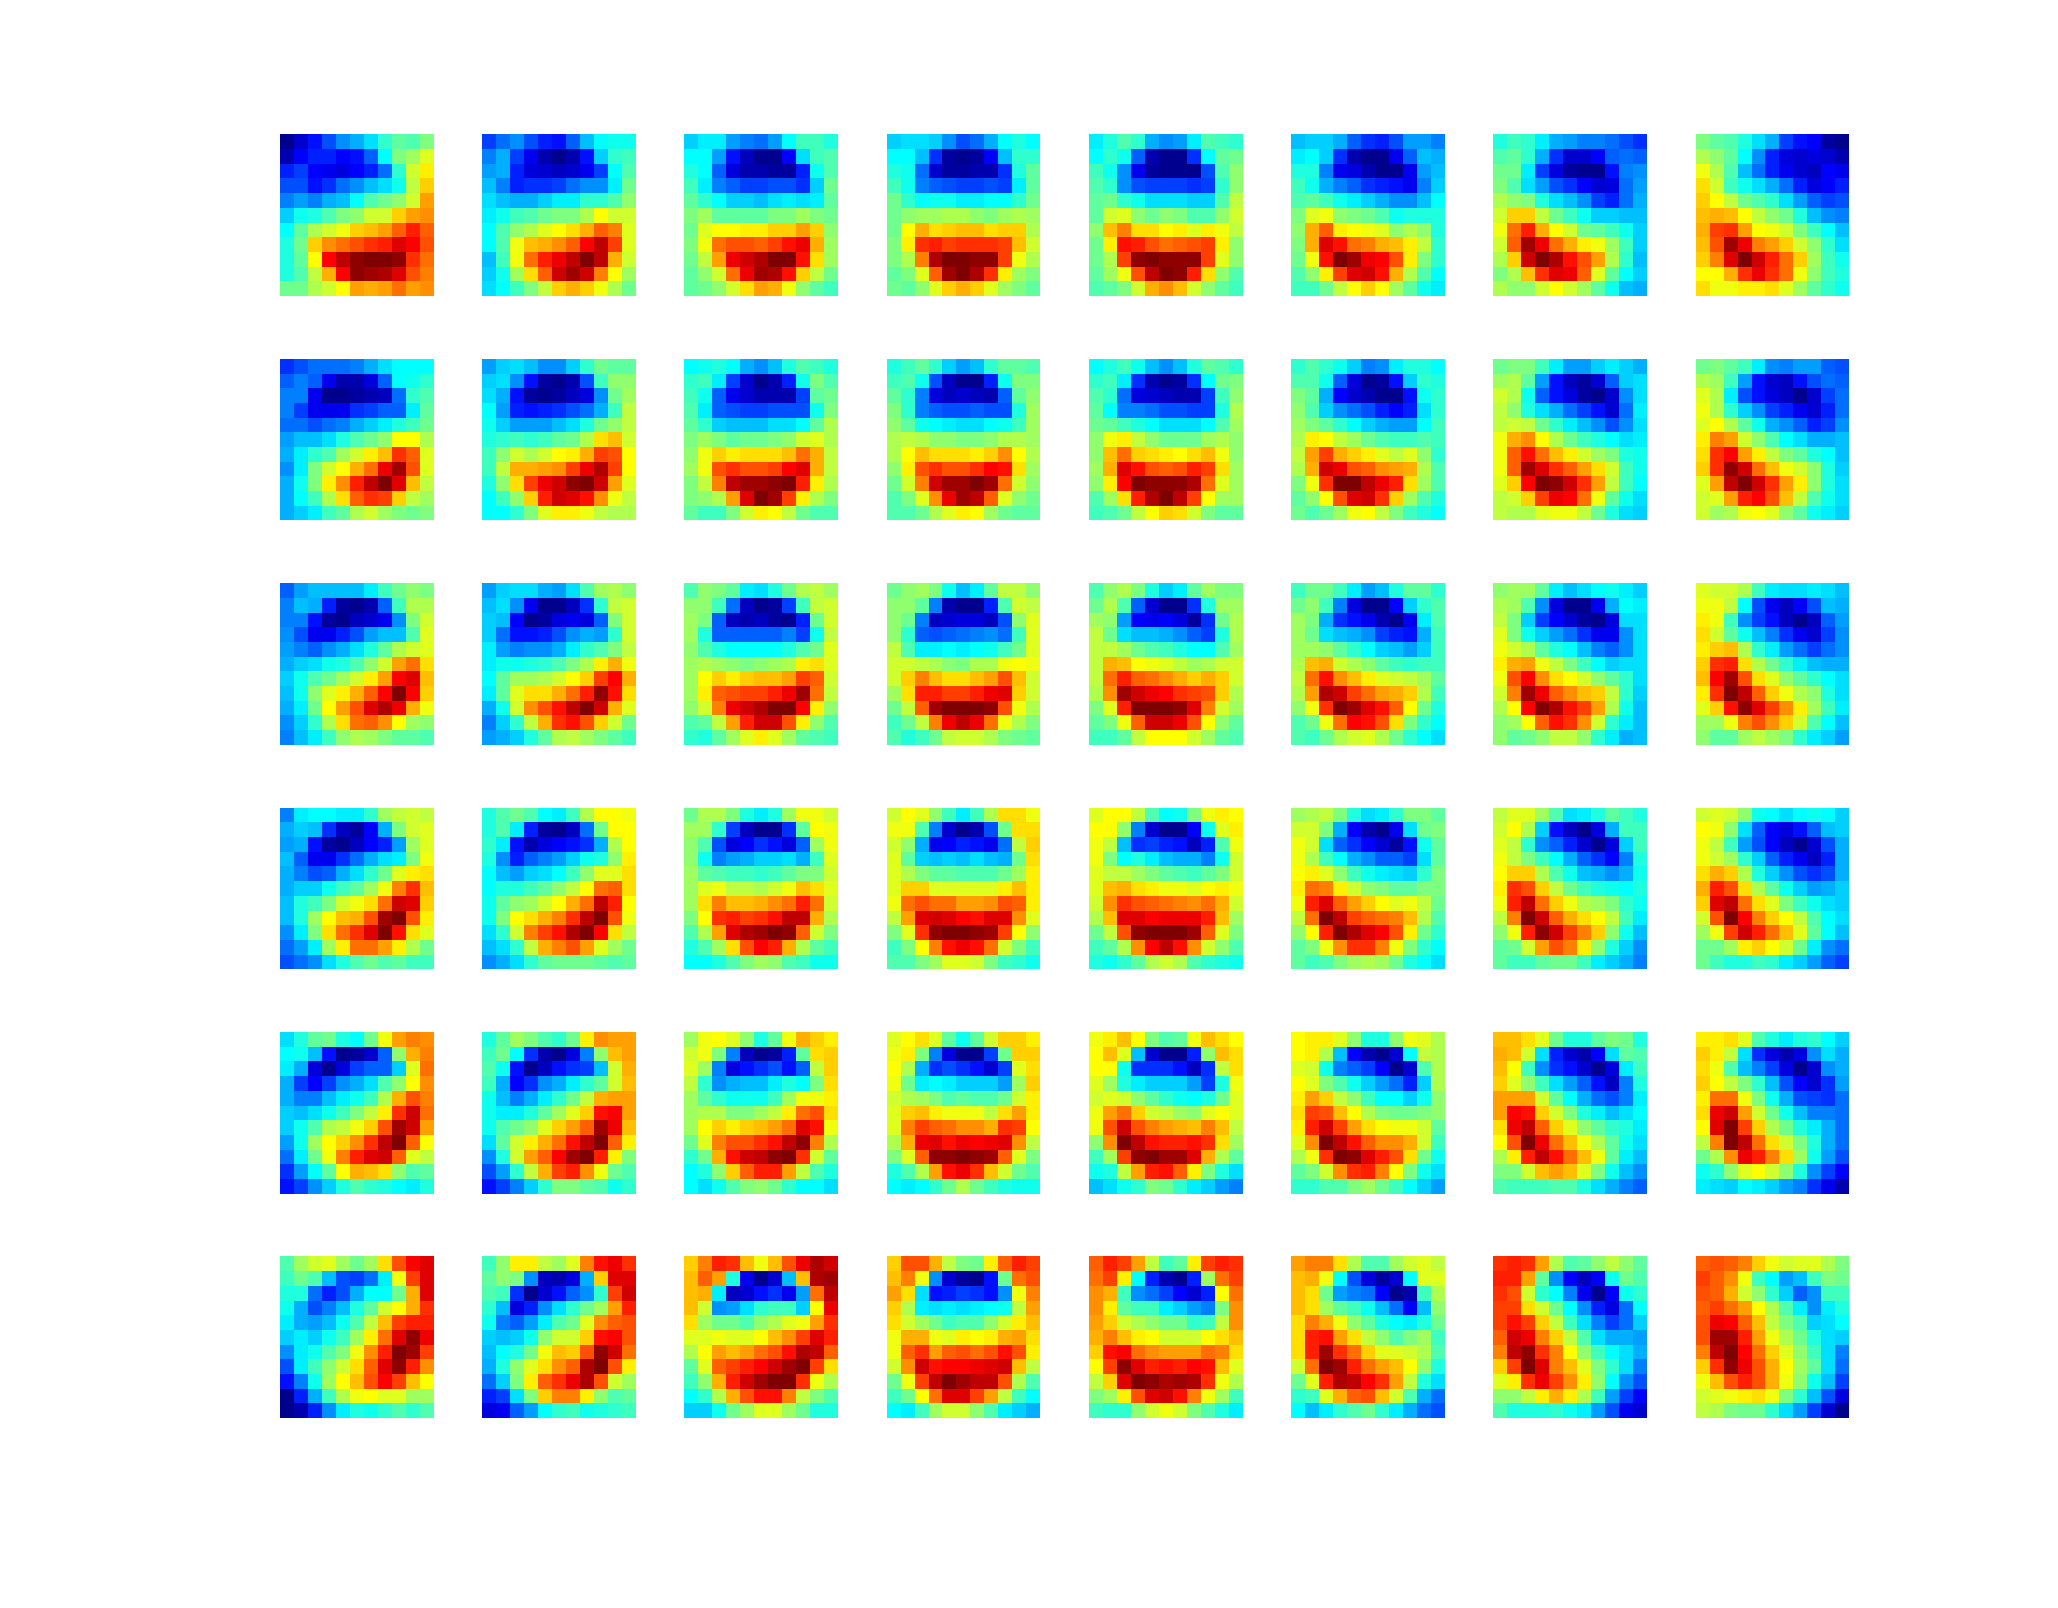
\includegraphics[width=\textwidth]{mean_scallop_quadrants}
      \caption{}
      \label{subfig:mean_quadrant}
  \end{subfigure}
  \begin{subfigure}[]{0.45\textwidth}
      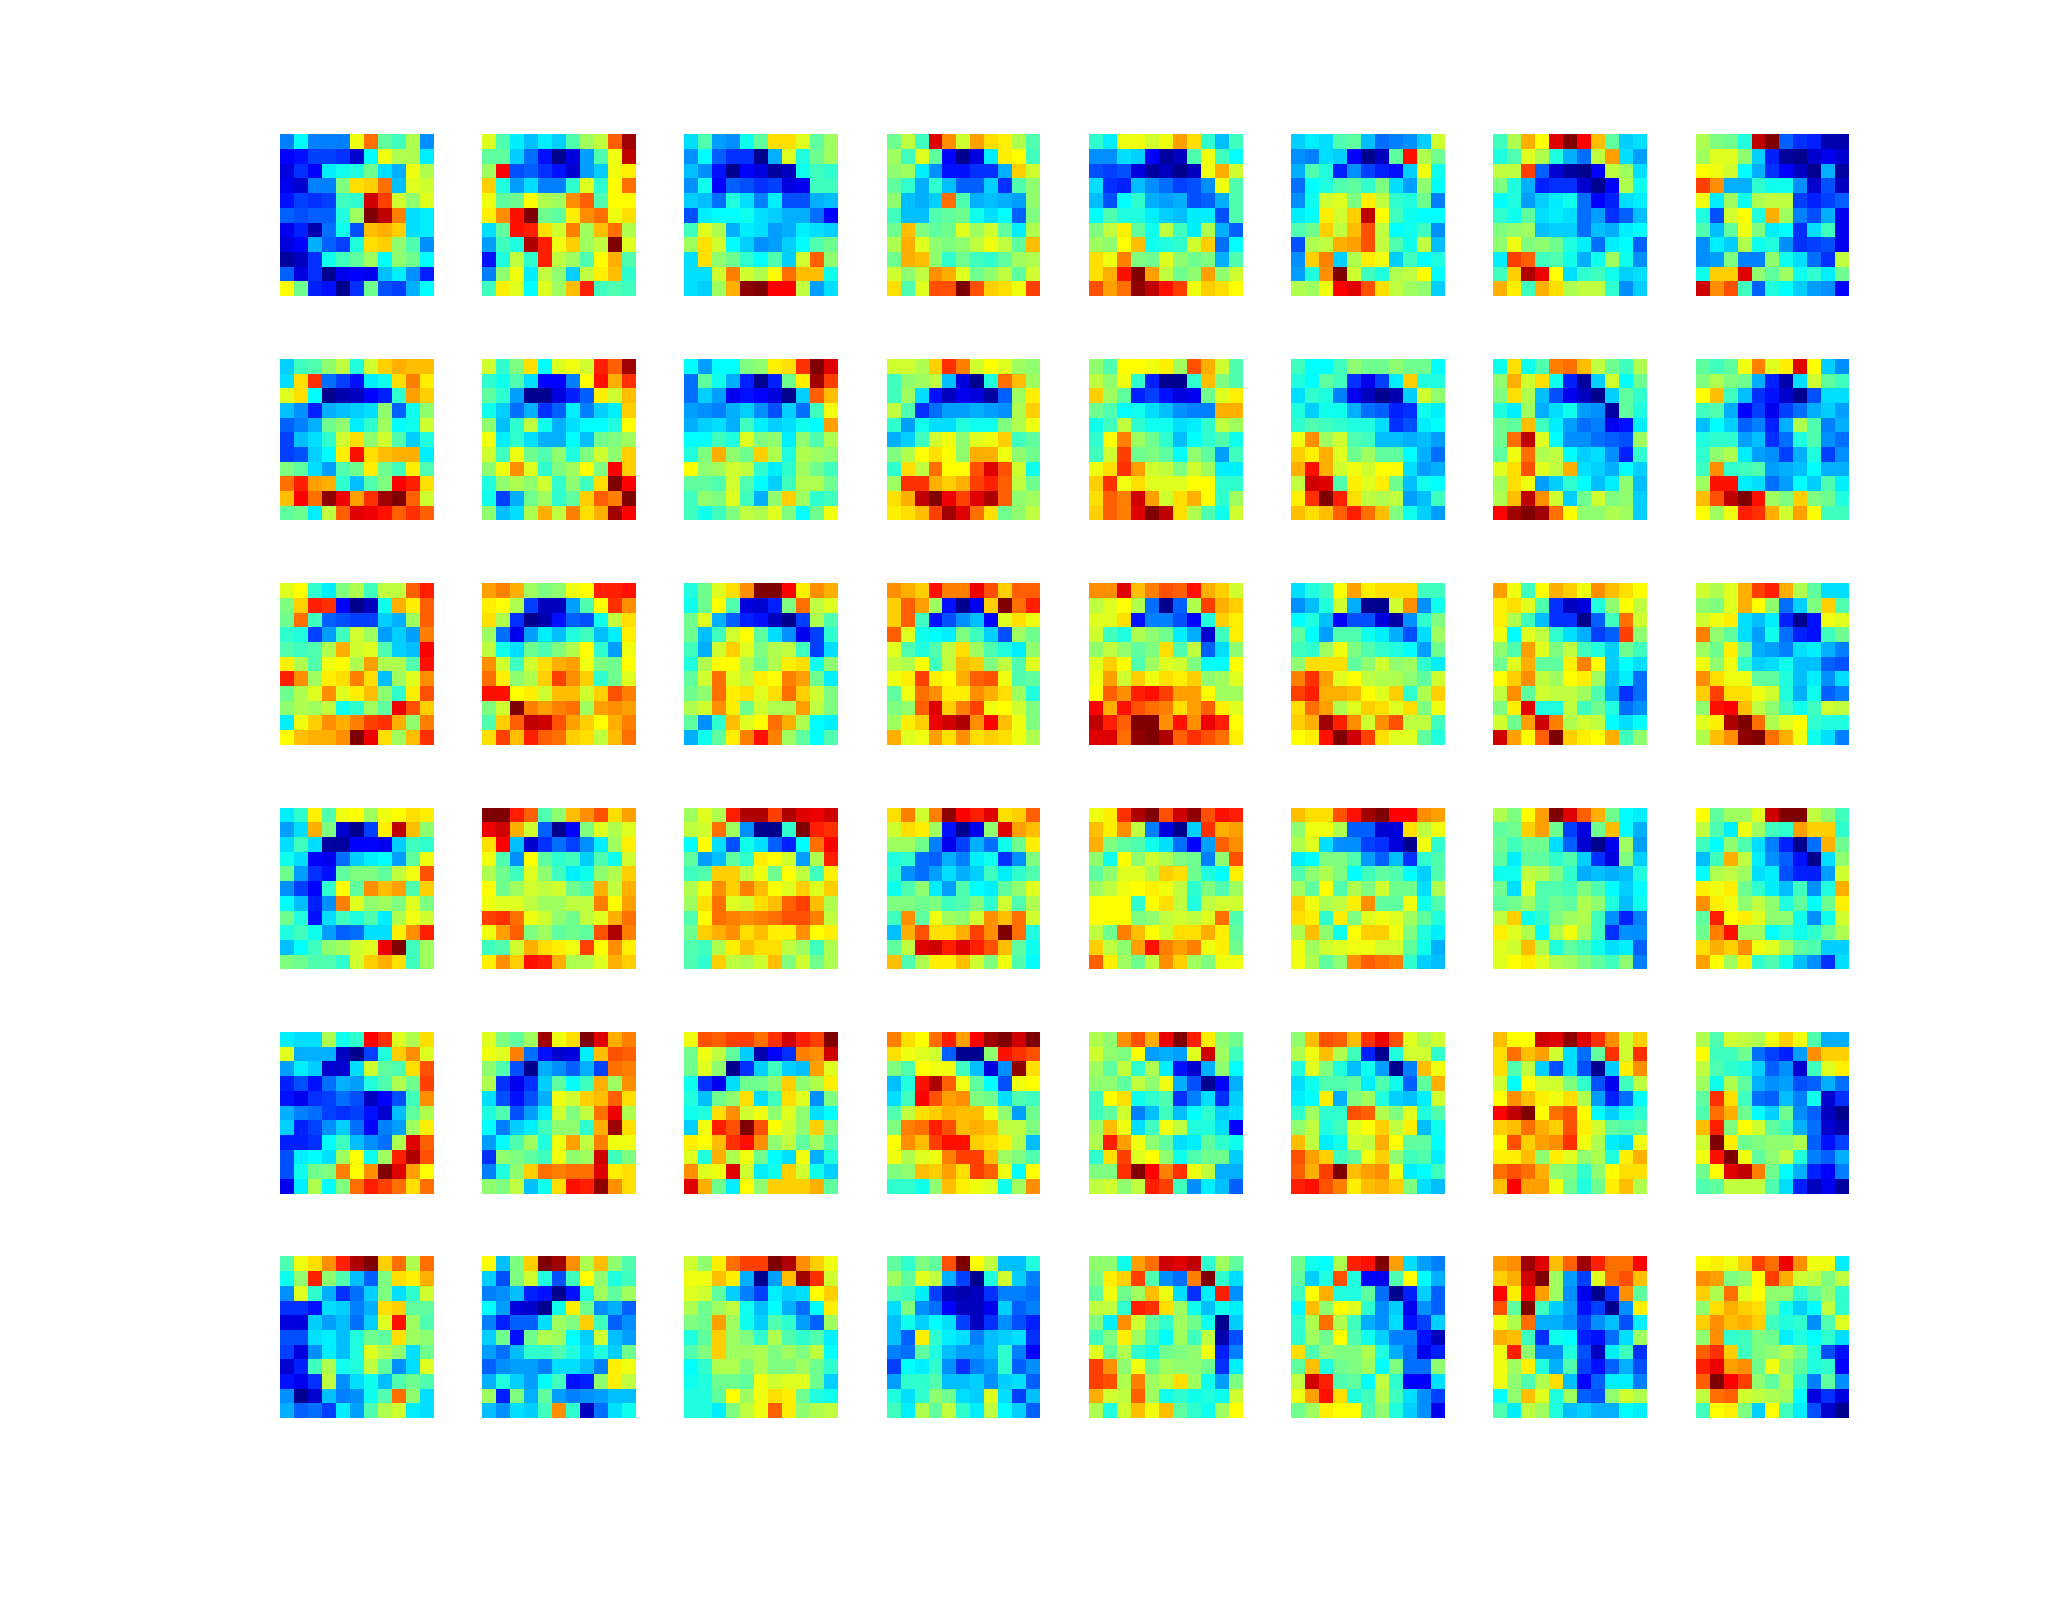
\includegraphics[width=\textwidth]{stddev_scallop_quadrants}        
      \caption{}
      \label{subfig:stddev_quadrant}
  \end{subfigure}
  \caption[Mean and variance map of scallops in each quadrant]{(\subref{subfig:mean_quadrant}) Mean map of scallops in each quadrant; (\subref{subfig:stddev_quadrant}) Standard deviation map of scallops in each quadrant.
  Red corresponds to higher numeric values and blue correspond to lower numeric values.}
  \label{fig:mean_stddev_quadrant}
\end{figure*}



\subsubsection{Scallop Profile Learning} \label{subsubsec:scallop_profile_learning}

The statistics of the dataset of $3\,706$ images used to produce Figure~\ref{fig:mean_stddev_quadrant} form a look-up table that represents reference scallop profile (mean and standard deviation maps) 
as a function of scallop center pixel location.
To obtain the reference profile for a pixel location, 
the statistics from all the scallops whose centers lie inside a $40\times40$ window centered on the pixel is used.
This look-up table can be compressed; it turns out that not all of the 121 bins ($11\times11$) within each map is equally informative, because bins close to the boundary are more likely to include a significant number of background pixels.
For this reason, a circular mask with a radius covering 4 bins is applied to each map (Figure~\ref{fig:scallop_learning_mask}), thus reducing the number of bins that are candidates as features for identification to $61$.
Out of these $61$ bins, $15$ additional bins having the highest standard deviation are ignored, leading to a final set of $46$ bins.
The value in the selected $46$ bins from mean map forms a $46$-dimensional feature vector associated with that region. The corresponding $46$ bins from the standard deviation map are also recorded, and are used to weight the features
(as seen later in \eqref{distance}).

\begin{figure}
  \centering
  \begin{subfigure}[]{0.3\textwidth}
      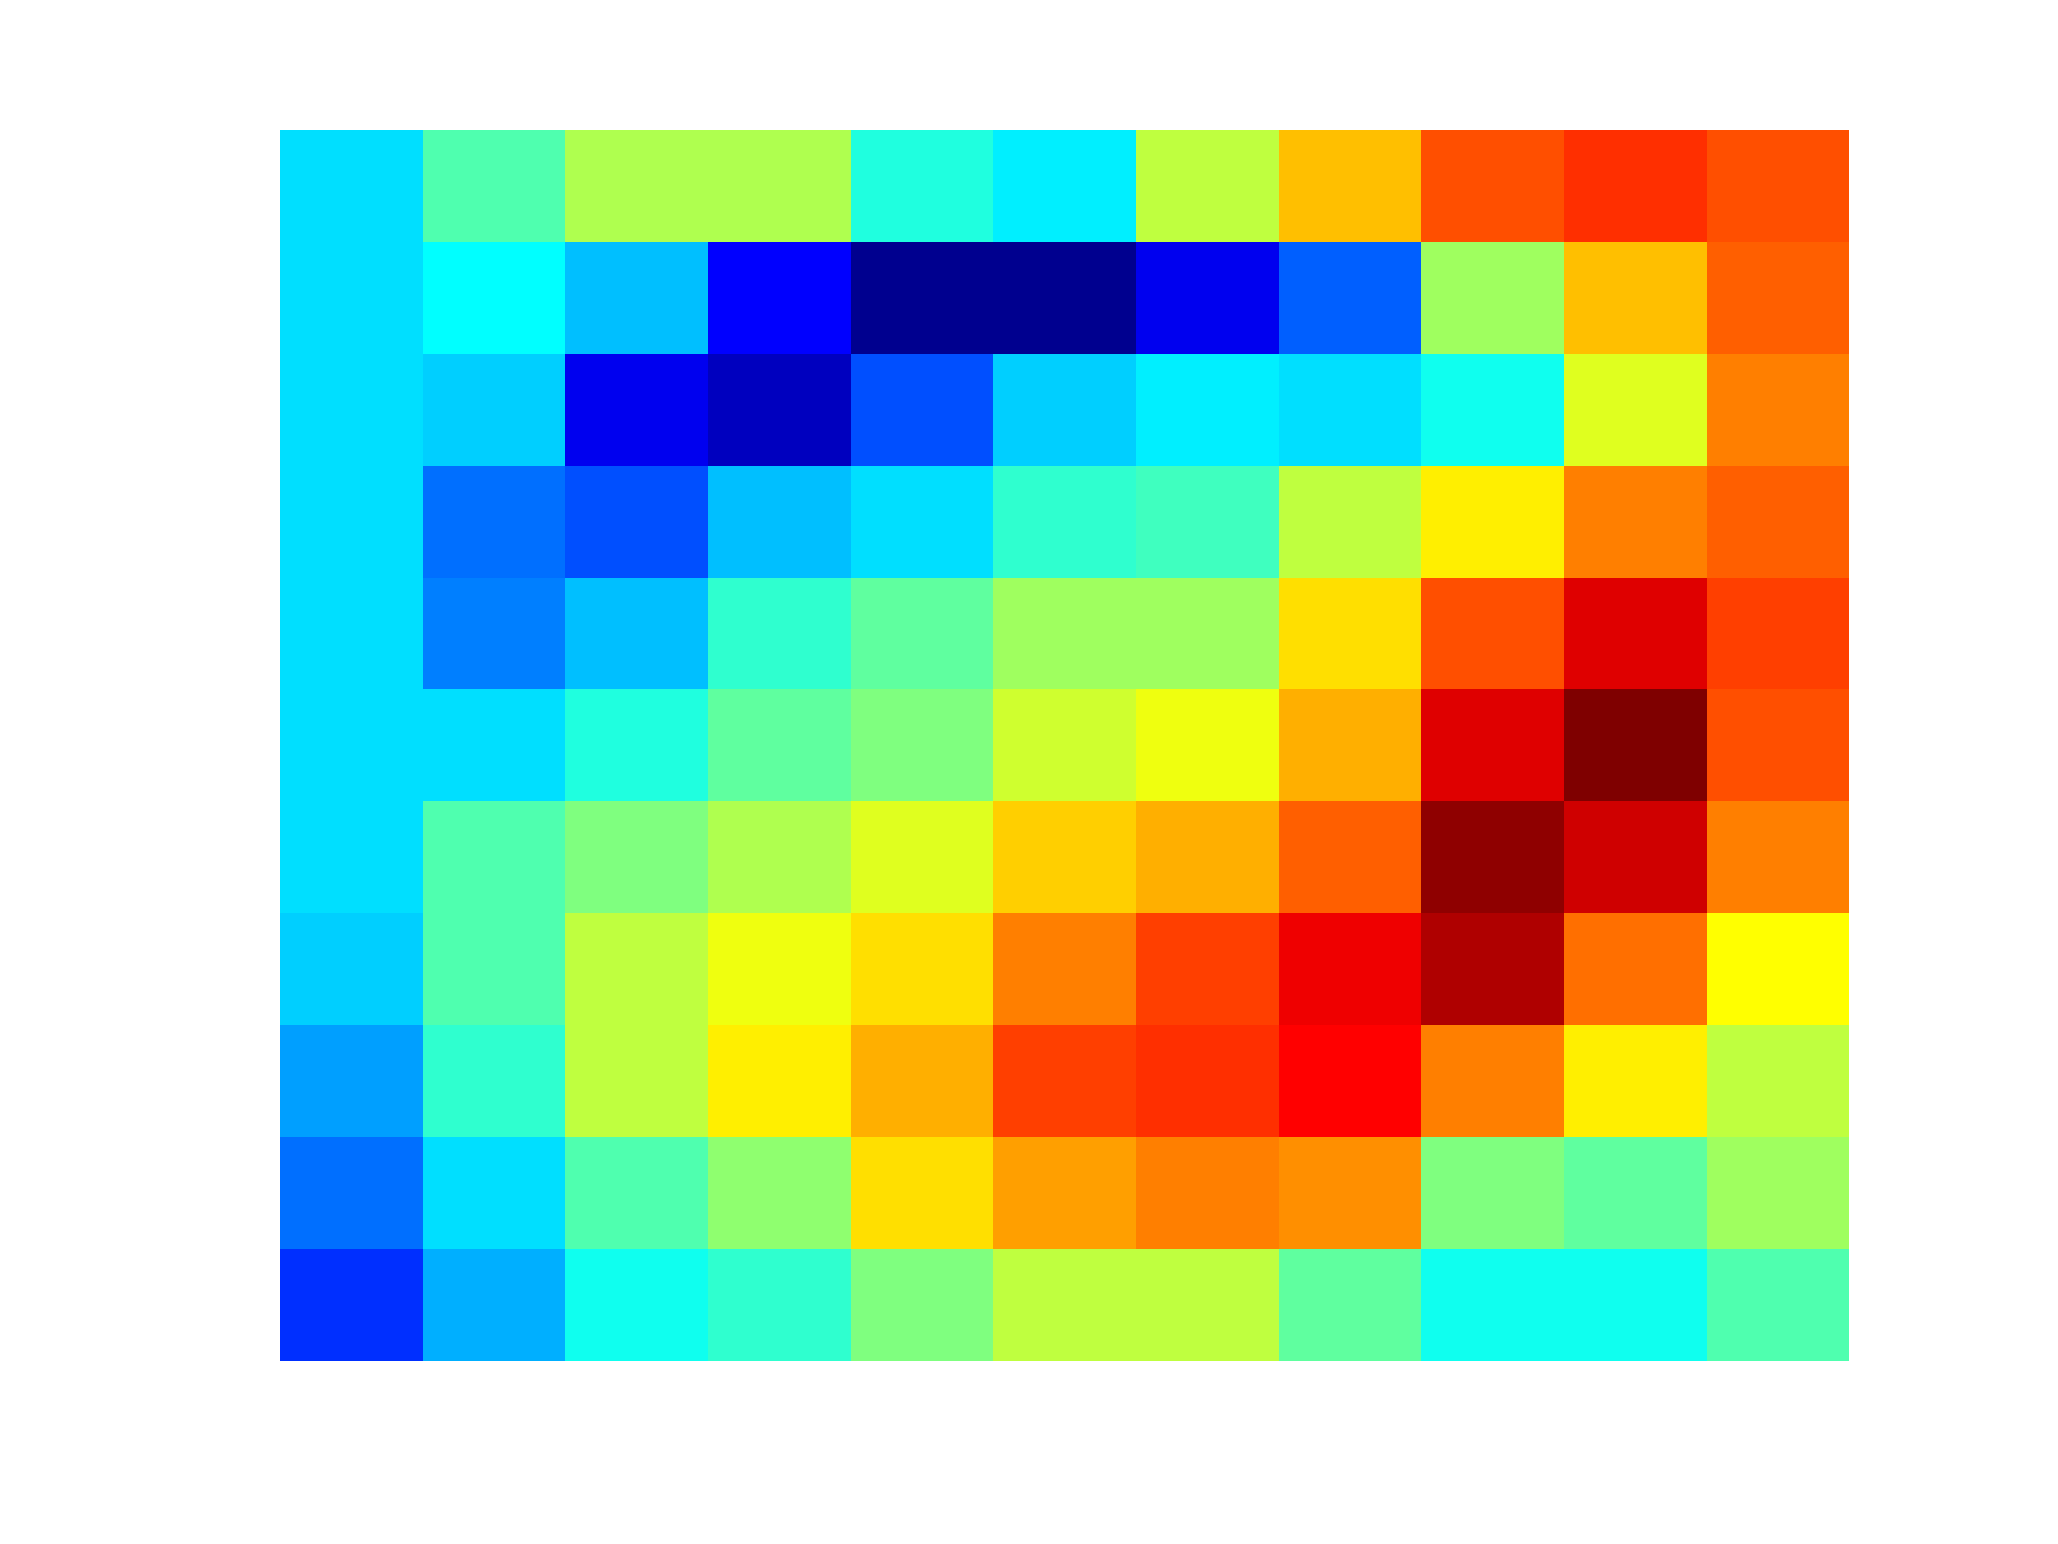
\includegraphics[width=\textwidth]{curr_scallop_mean}
      \caption{}
      \label{subfig:mean_scallop}
  \end{subfigure}
  \begin{subfigure}[]{0.3\textwidth}
      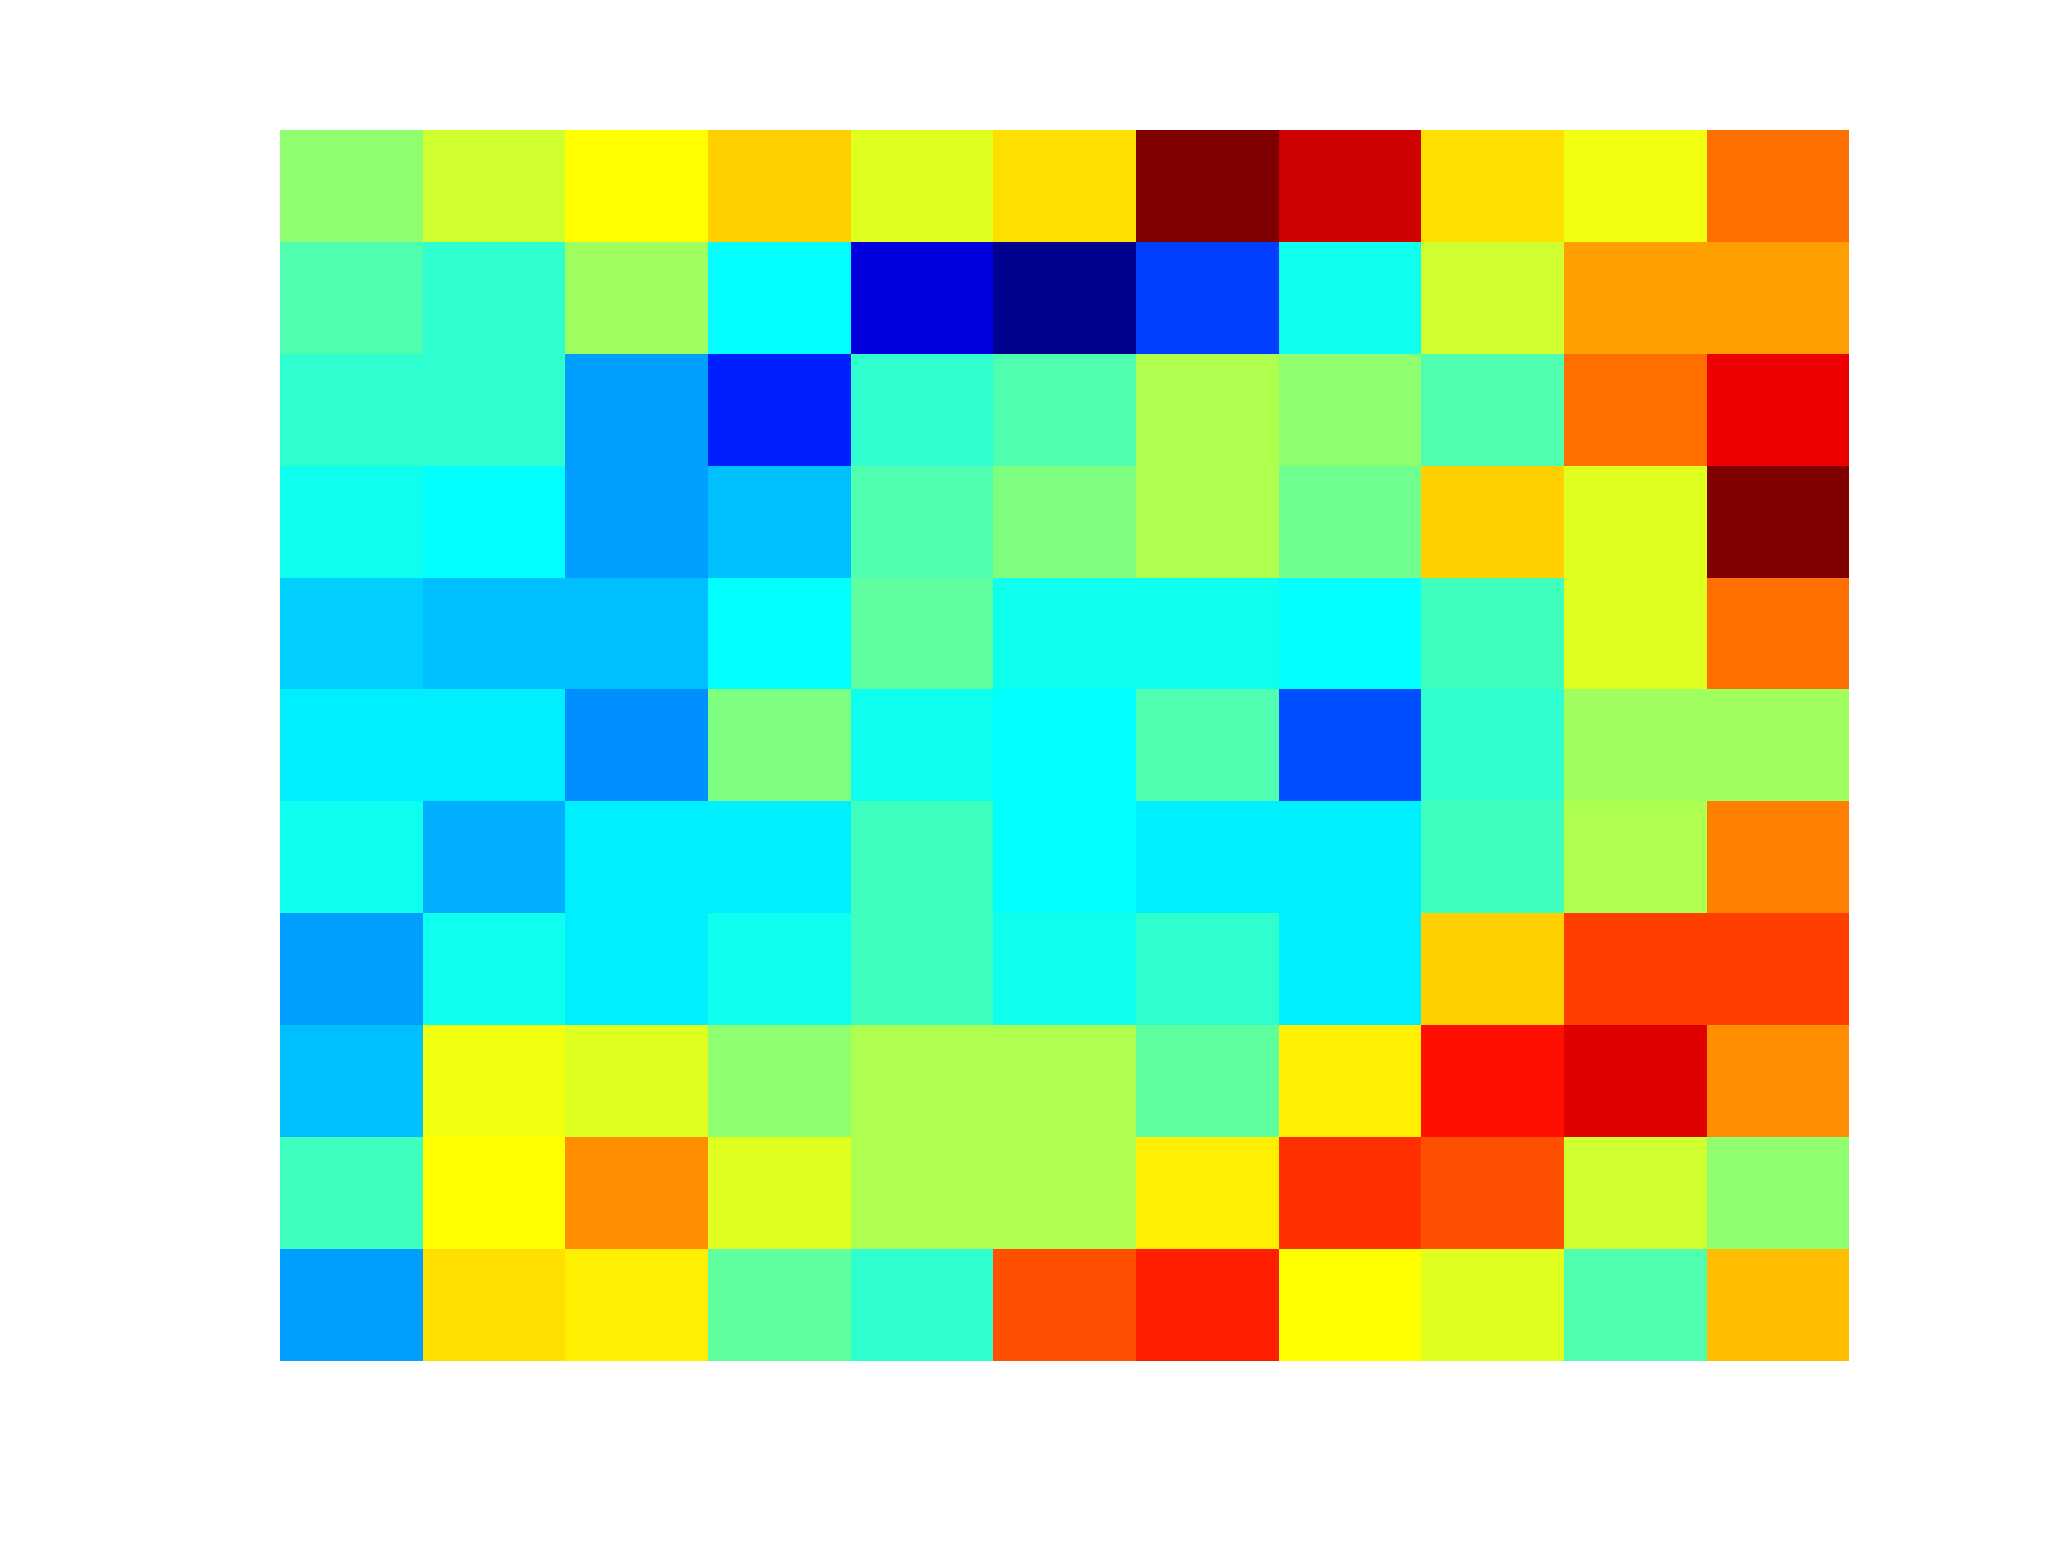
\includegraphics[width=\textwidth]{curr_scallop_stddev}
      \caption{}
      \label{subfig:stddev_scallop}
  \end{subfigure}
  \begin{subfigure}[]{0.3\textwidth}
      
\includegraphics[width=\textwidth]{mask_centered}
      \caption{}
      \label{subfig:mask_scallop}
  \end{subfigure}
  \caption[Illustration of scallop profile hypothesis]{Intensity statistics and mask for a region centered at image coordinates $(470,63)$: (\subref{subfig:mean_scallop}) Map of mean intensity; (\subref{subfig:stddev_scallop}) Map of intensity standard deviation;
  (\subref{subfig:mask_scallop}) Mask applied to remove background points.}
  \label{fig:scallop_learning_mask}
\end{figure}


\subsubsection{Scallop Template Matching} \label{subsubsec:scallop_template_matching}

With this look-up table that codes the reference scallop profile for every scallop center pixel location,
the resemblance of any segmented object to a scallop can now be assessed.
The metric used for this comparison is a weighted distance function between the 
elements of the feature vector for the region corresponding to the segmented object, and that coming from the look-up table, depending on the location of the object in the image being processed.
If this distance metric is below a certain threshold $D_\mathsf{thresh}$, the object is classified
a scallop.
Technically, let $X^o=(X^o_1,X^o_2, \ldots,X^o_{46})$ denote the feature vector computed for the segmented object,
and $X^s=(X^s_1,\ldots,X^s_{46})$ the reference
feature vector. 
Every component of the $X^s$ vector is a reference mean intensity value for a particular bin, and is associated with a standard deviation $\sigma_k$ from the reference standard deviation map.
%(Section~\ref{subsubsec:scallop_profile_hypothesis}).
To compute the distance metric, first normalize $X^o$ to produce vector $X^{\bar{o}}$ with components 
%
\[
X^{\bar{o}}_p = \min_{k} X^s_k + \left(\frac{\max \limits_{k} X^s_k-\min \limits_{k} X^s_k}{\max \limits_{k} X^o_k-\min \limits _{k} X^o_k}
\right)\left[ X^o_p-\min_{k} X^o_k \right] \;\text{for } p=1,\ldots,46\enspace,
\]
%
and then evaluate the distance metric $D_{t}$ quantifying the dissimilarity between the normalized object vector $X^{\bar{o}}$ and the reference feature vector $X^s$ as
%
\begin{equation}\label{distance}
D_{t} = \sqrt{\sum_{k=1}^n\frac{\|X^{\bar{o}}_{k}-X^s_k\|^2}{\sigma_k}} \enspace .
\end{equation}
%

%
\begin{figure}
\centering
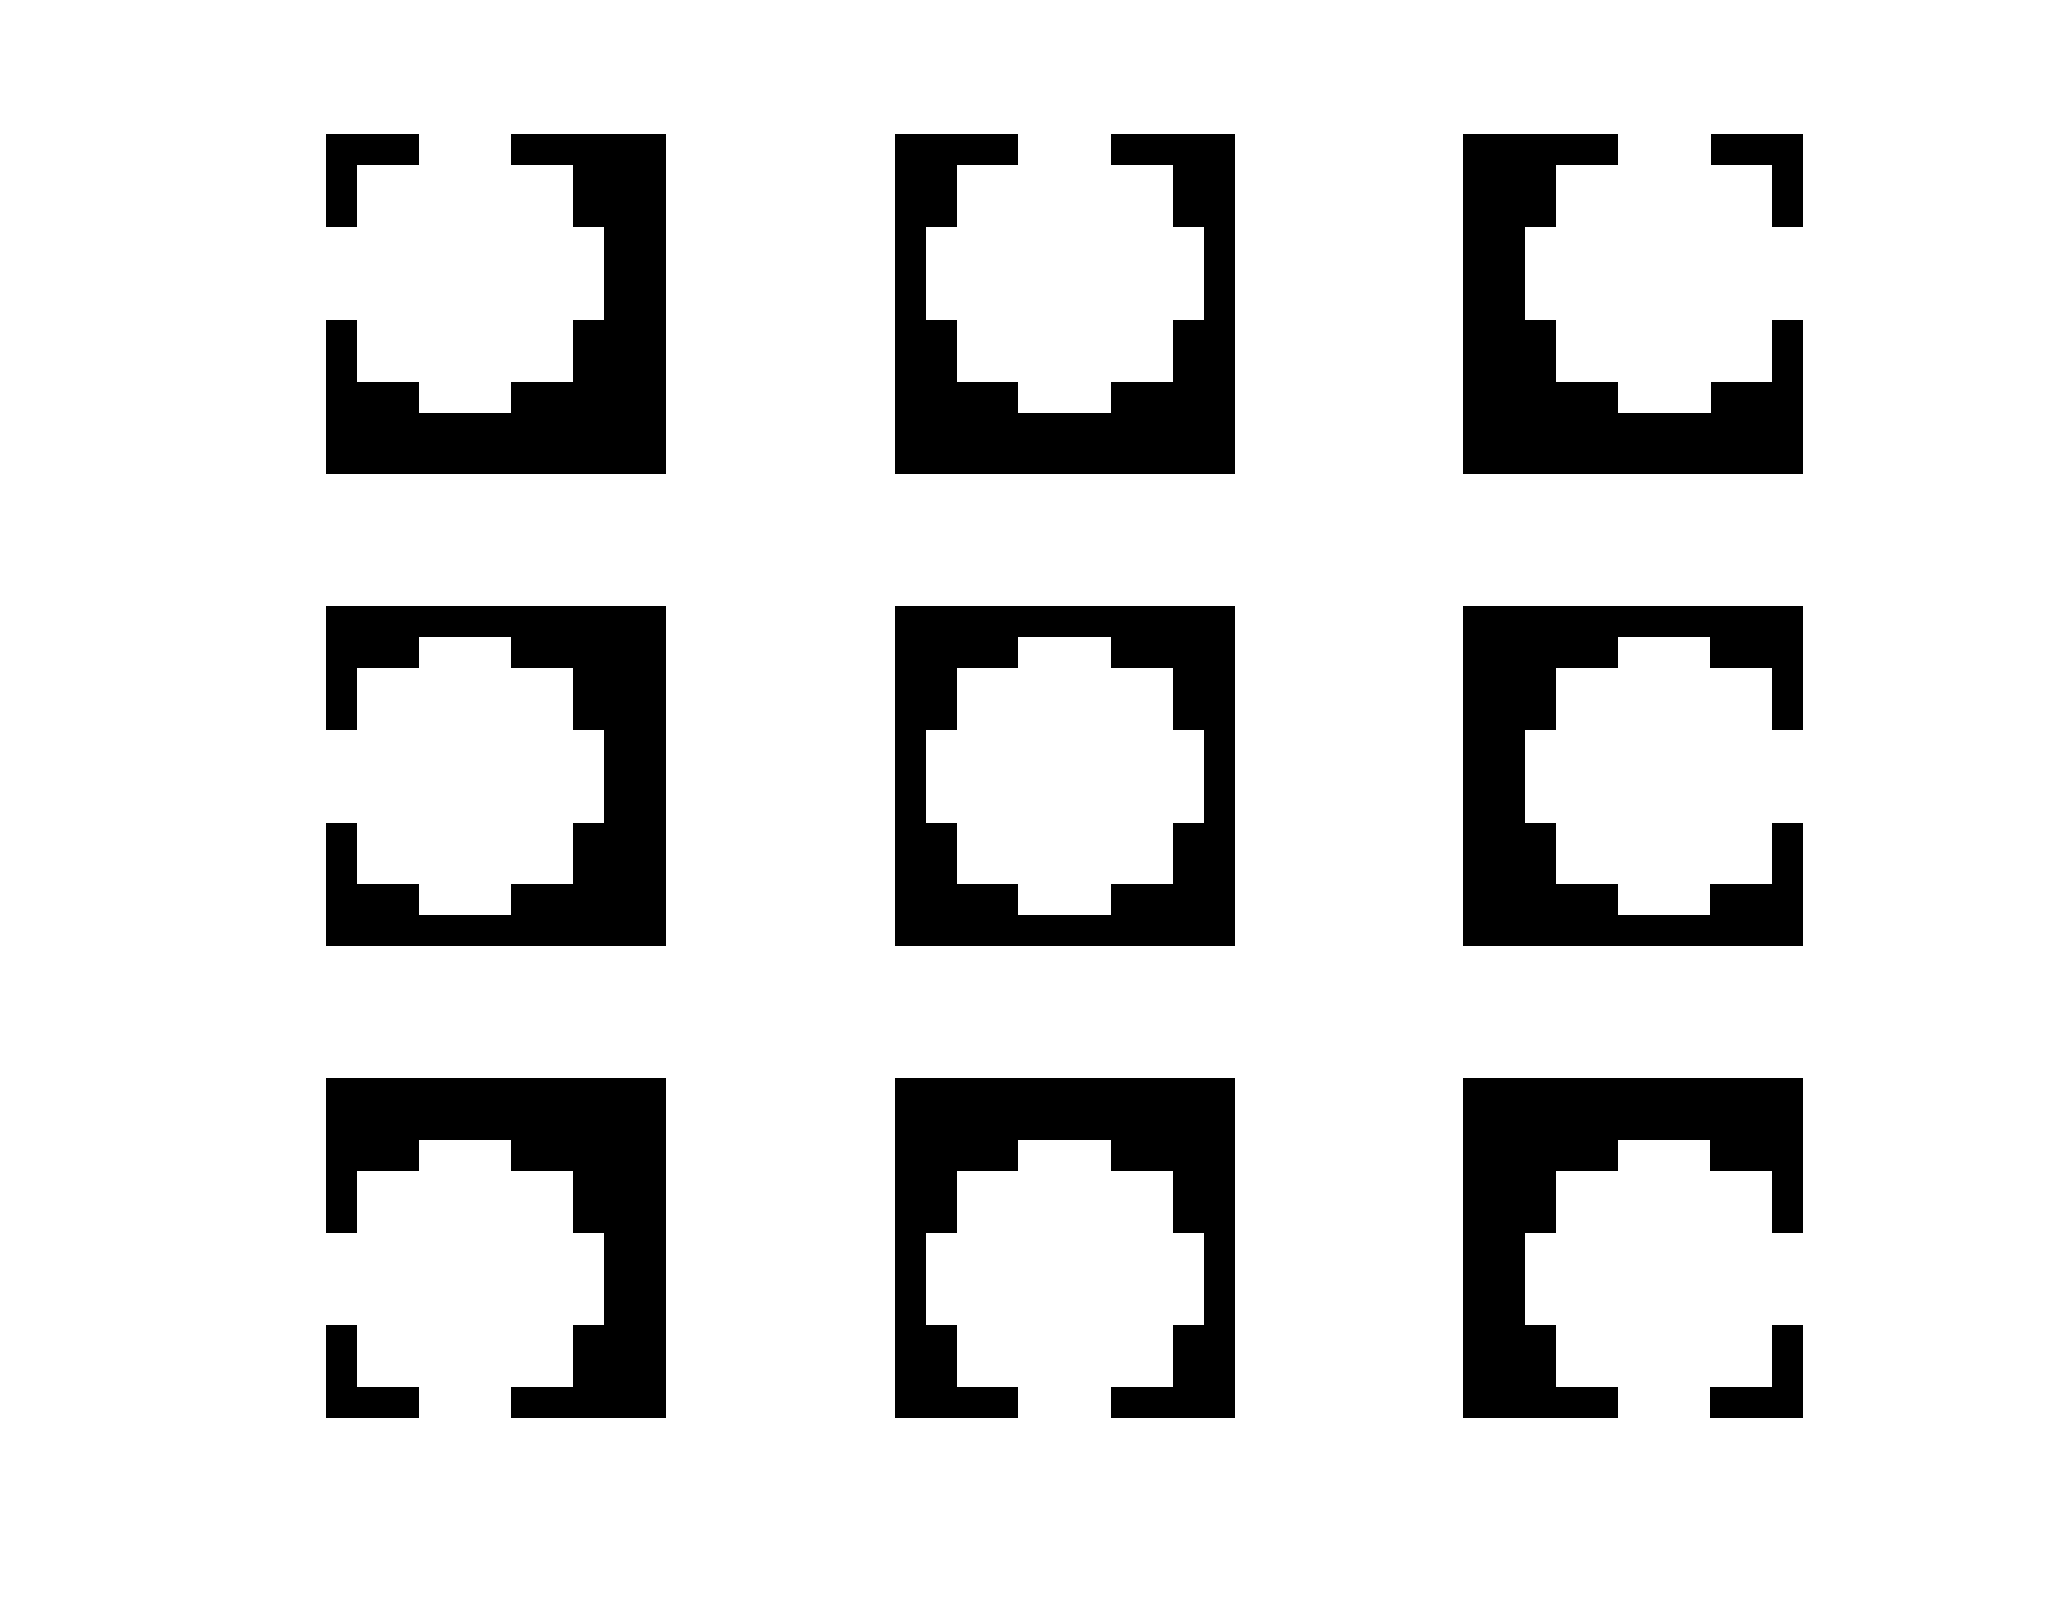
\includegraphics[width=0.6\textwidth]{mask_offset}
\caption[Template matching masks]{Nine different masks slightly offset from the center used to make the classification layer
robust to errors in segmentation}
\label{fig:scallop_masks}
\end{figure}
%

Small variations in segmentation can produce notable deviations in the computed distance metric \eqref{distance}.
To alleviate this effect, the mask of Figure~\ref{subfig:mask_scallop} was slightly shifted in different directions and the best match in terms of the distance was identified.
This process enhanced the robustness of the classification layer with respect to  small segmentation errors.
Specifically, nine slightly shifted masks were used (shown in
Figure~\ref{fig:scallop_masks}).  Out of the nine resulting
distance metrics $D^{o_1}_t$ \ldots $D^{o_9}_t$, the smallest $
 D_\mathsf{obj}=\min_{p\in\{1,\ldots,9\}} D^{o_p}_t
$ is found and used for classification. 
If $D_\mathsf{obj}<D_\mathsf{thresh}$, 
the corresponding object
is classified as a scallop.
Based on Figures~\ref{subfig:precision_recall}--\ref{subfig:template_hist},
the threshold value was chosen at $D_\mathsf{thresh}=7$ to give a recall\footnote{\emph{Recall} refers to the fraction of relevant instances
identified: fraction of scallops detected over all ground truth scallops;
\emph{precision} is the fraction of the instances returned that are really relevant
compared to all instances returned: fraction of true scallops over all objects
identified as scallops.} rate of 
$97\%$.
Evident in Figure~\ref{subfig:precision_recall} is the natural trade-off between increasing recall rates and keeping the number of false positives low.

%
\begin{figure*}
  \centering
  \begin{subfigure}{0.47\textwidth}
      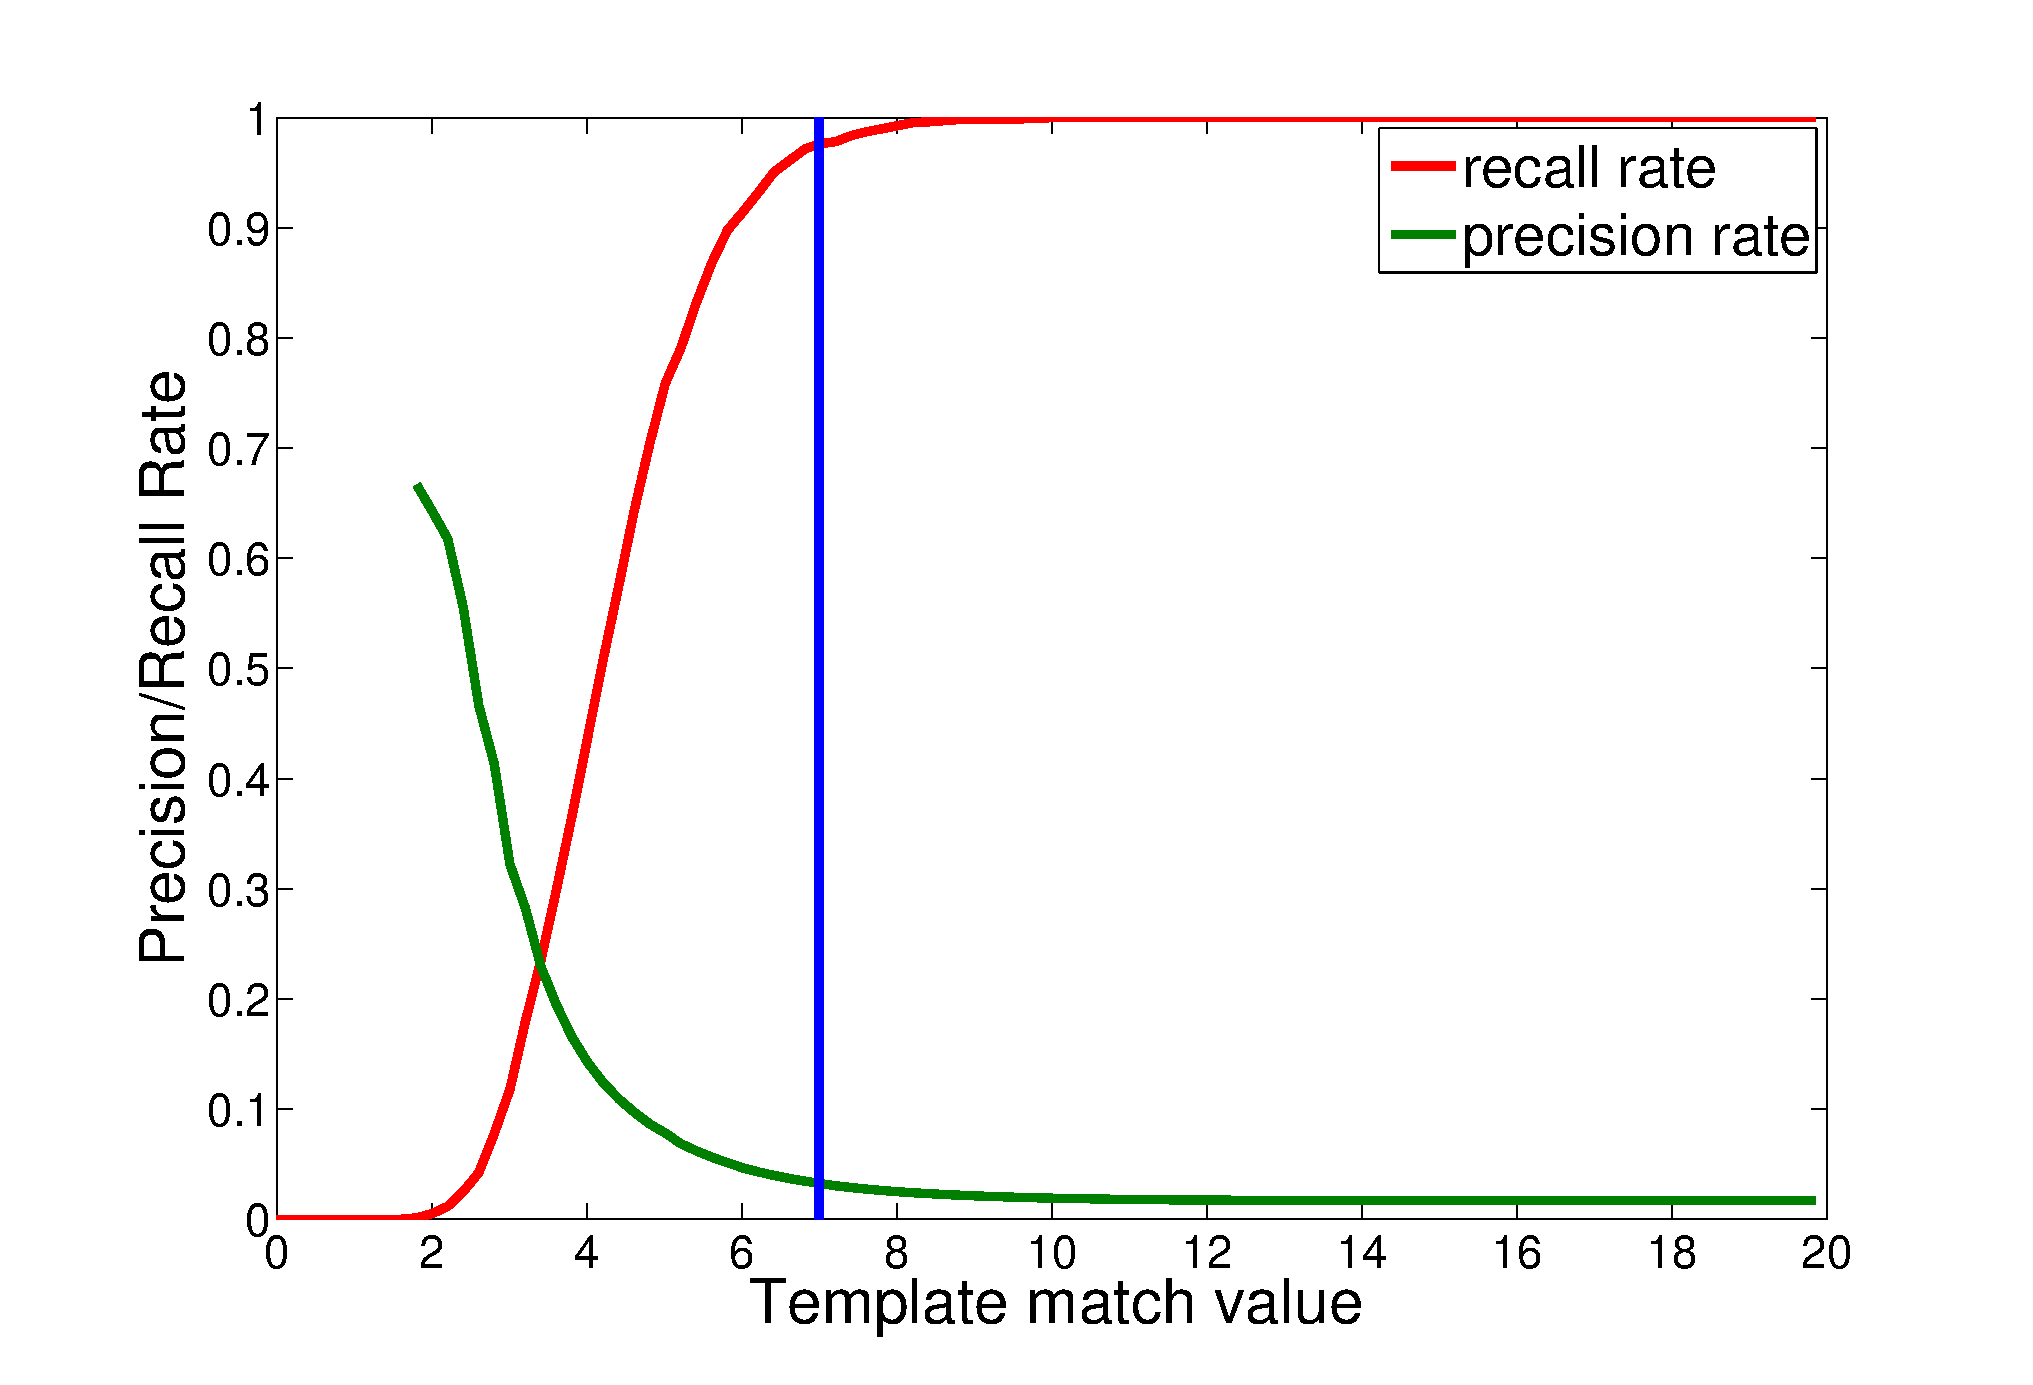
\includegraphics[width=\textwidth]{precision_recall}
      \caption{}
      \label{subfig:precision_recall}
  \end{subfigure}
  \begin{subfigure}{0.47\textwidth}
      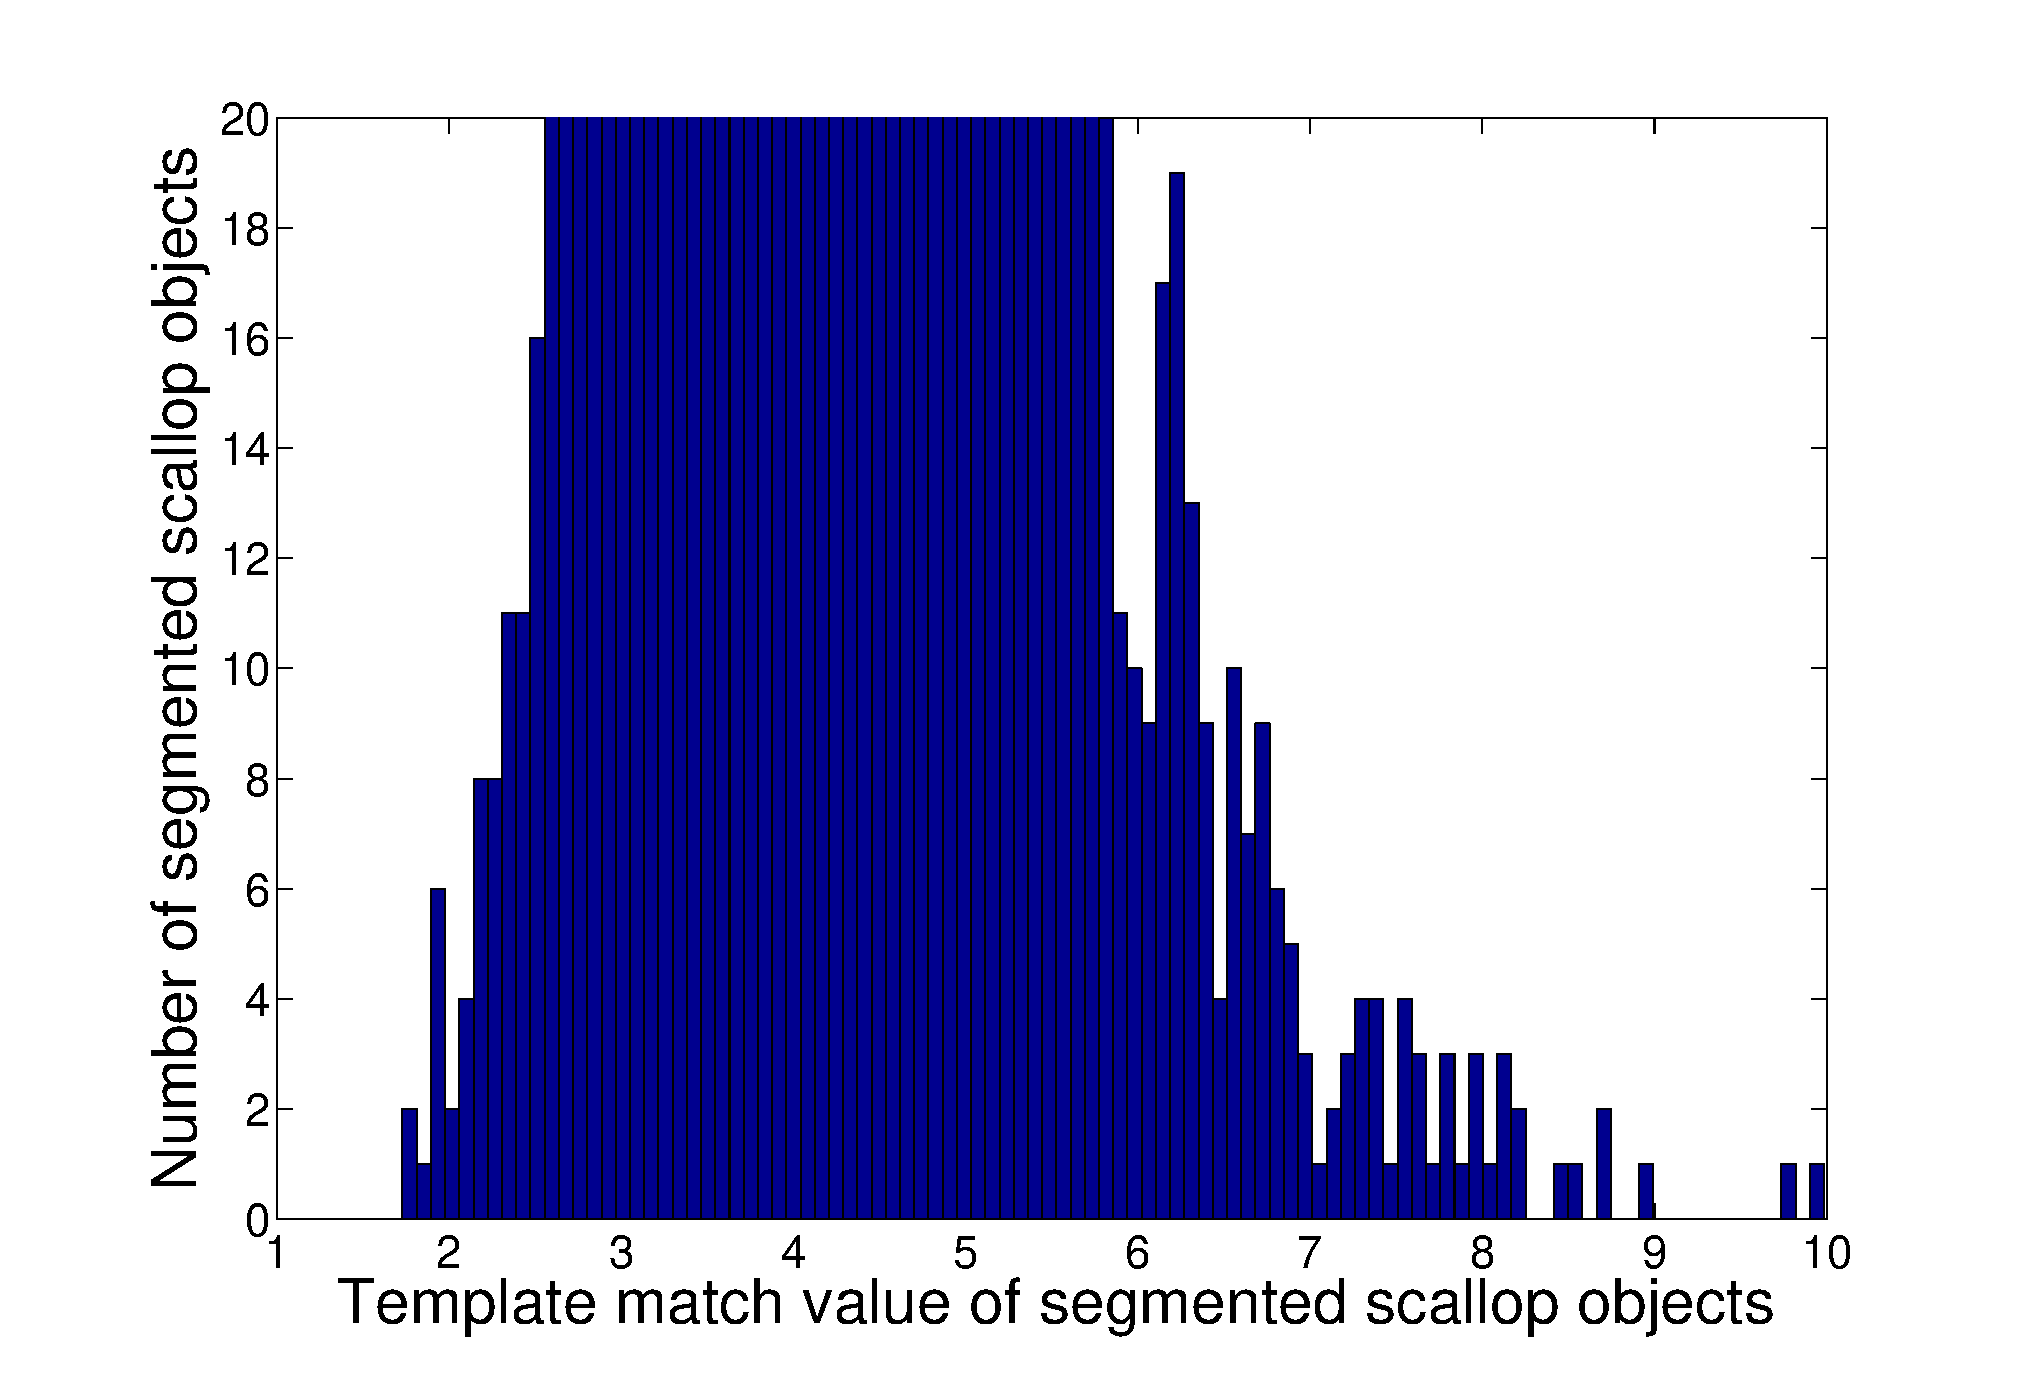
\includegraphics[width=\textwidth]{template_thresh_hist}         
      \caption{}
      \label{subfig:template_hist}
  \end{subfigure}
  \caption[Precision-Recall curves for Classification Layer]{(\subref{subfig:precision_recall}) Precision-Recall curve with $D_\mathsf{thresh}$ shown as
  a vertical line; (\subref{subfig:template_hist}) 
  Histogram of template match of segmented scallop objects.}
  \label{detection-curves}
\end{figure*}
%========================================================================================
\subsection{Layer IV: False Positives Filter}

To decrease the false positives that are produced in the classification layer, two methods are evaluated as possible candidates: a high-dimensional \gls{wctm} technique and a \gls{hog} method. 
The main objective here is to find a method that will retain a high percentage of true positive scallop and at the same time eliminate as many false positives from the classification layer as possible.

\subsubsection{High-dimensional weighted correlation template matching (WCTM)}
In this method, the templates used are generated from scallop images that are \emph{not} preprocessed, i.e., images that are not median-filtered, unlike the images that were processed by the first three layers. 
The intuition behind this is that although median filtering reduces speckle noise and may improve the performance of segmentation, it also weakens the edges and gradients in an image. 
Avoiding median filtering helps to generate templates that are more accurate than the ones already used in the classification layer.

Based on the observation that the scallop templates are dependent on their position in the image (Figure~\ref{fig:mean_stddev_quadrant}), a new scallop template is generated for each object that is classified as a scallop in Layer III. 
As indicated before, such an object would be represented by a triplet $(a_o,b_o,R_o)$, where $a_o$ and $b_o$ represent the spatial Cartesian coordinates of object's geometric center, and $R_o$ gives its radius. 
The representative scallop template is now generated from all scallops in the learning set (containing 3\,706 scallops), of which the center is within a $40\times40$ window in the neighborhood of the object center $(a_o,b_o)$. 
Each of these scallops is then extracted using a window of size $2.5R\times2.5R$ where $R$ is the scallop radius. 
Since these scallops in the learning set can be of different dimensions, it is resized (scaled) to a window of size $2.5R_o\times2.5R_o$. 
All these scallop instances in the learning set are finally combined through a pixel-wise mean to obtain the mean representative template. 
Similarly, a standard deviation map that captures the standard deviation of each pixel in the mean template is also obtained.  
The templates produced here are of larger size compared to the templates in Layer III (recall that a Layer III template was of size $11\times11$).
The inclusion of slightly more information contributes to these new larger templates being more accurate.

In a fashion similar to the analysis in Layer III, the templates and object pixels first undergo normalization and mean subtraction.
Then they are compared.
Let $v=(2.5R_o)^2$ be the total number of pixels in both the template and the object, and let the new reference scallop feature (template) and the object be represented by vectors $X^t=(X^t_1,X^t_2, \ldots,X^t_{v})$ and $X^u=(X^u_1,\ldots,X^u_{v})$, respectively. 
In addition, let $\sigma$ be the standard deviation vector associated with $X^t$.
Then the reference scallop feature vector $X^t$ would first be normalized as follows: 
%
\[
X^{t'}_p = \min_{k} X^u_k + \left(\frac{\max \limits_{k} X^u_k-\min \limits_{k} X^u_k}{\max \limits_{k} X^{t}_k-\min \limits _{k} X^{t}_k}
\right)\left[ X^{t}_p-\min_{k} X^{t}_k \right] \; ,
\]
%
where $p$ denotes the position of component $X^t_p$ in vector $X^t$.
Normalization is followed by mean subtraction, this time both for the template and for the object. 
The resulting, mean-subtracted reference scallop feature $X^{\bar{t}}$, and object $X^{\bar{u}}$ are computed as
%
\begin{align*}
X^{\bar{t}}_p &= X^{t'}_p-\frac{1}{v}\sum_{k=1}^{v}X^{t'}_k \enspace,& 
X^{\bar{u}}_p &= X^{u}_p-\frac{1}{v}\sum_{k=1}^{v}X^{u}_k \enspace.
\end{align*}
%
Now the standard deviation vector is normalized:
%
\[
\bar{\sigma}_p = \frac{\sigma_p}{\sum_{k=1}^{v}\sigma_k} \enspace.
\]
%
At this point, a metric that expresses the correlation between the mean-subtracted template and the object can be computed.
This metric is weighted by the (normalized) variance of each feature. 
In general, the higher the value of this metric, the better the match between the object and the template. 
The \gls{wctm} similarity metric is given by
%
\[
D_\mathsf{wctm} = \sum_{k=1}^v\frac{X^{\bar{t}}_{k}X^{\bar{u}}_k}{\bar{\sigma}_{k}} \enspace .
\]
%
The threshold set for the weighted correlation metric $D_\mathsf{wctm}$, in order to distinguish between likely true and false positives is at $0.0002222$, i.e., any object with a similarity score lower than this threshold is rejected. 
This threshold value is justified from the precision-recall curves (see Figure~\ref{subfig:layer4_precision_recall}) of the weighted correlation metric values for the objects filtering down from the classification layer. 
The threshold shown by the blue line corresponds to 96\% recall rate, i.e., 96\% of the true positive scallops from the classification layer pass through \gls{wctm}. 
At the same time, \gls{wctm} decreases the false positives by over 63\%.
%
\begin{figure}
  \centering
  \begin{subfigure}{0.45\textwidth}
      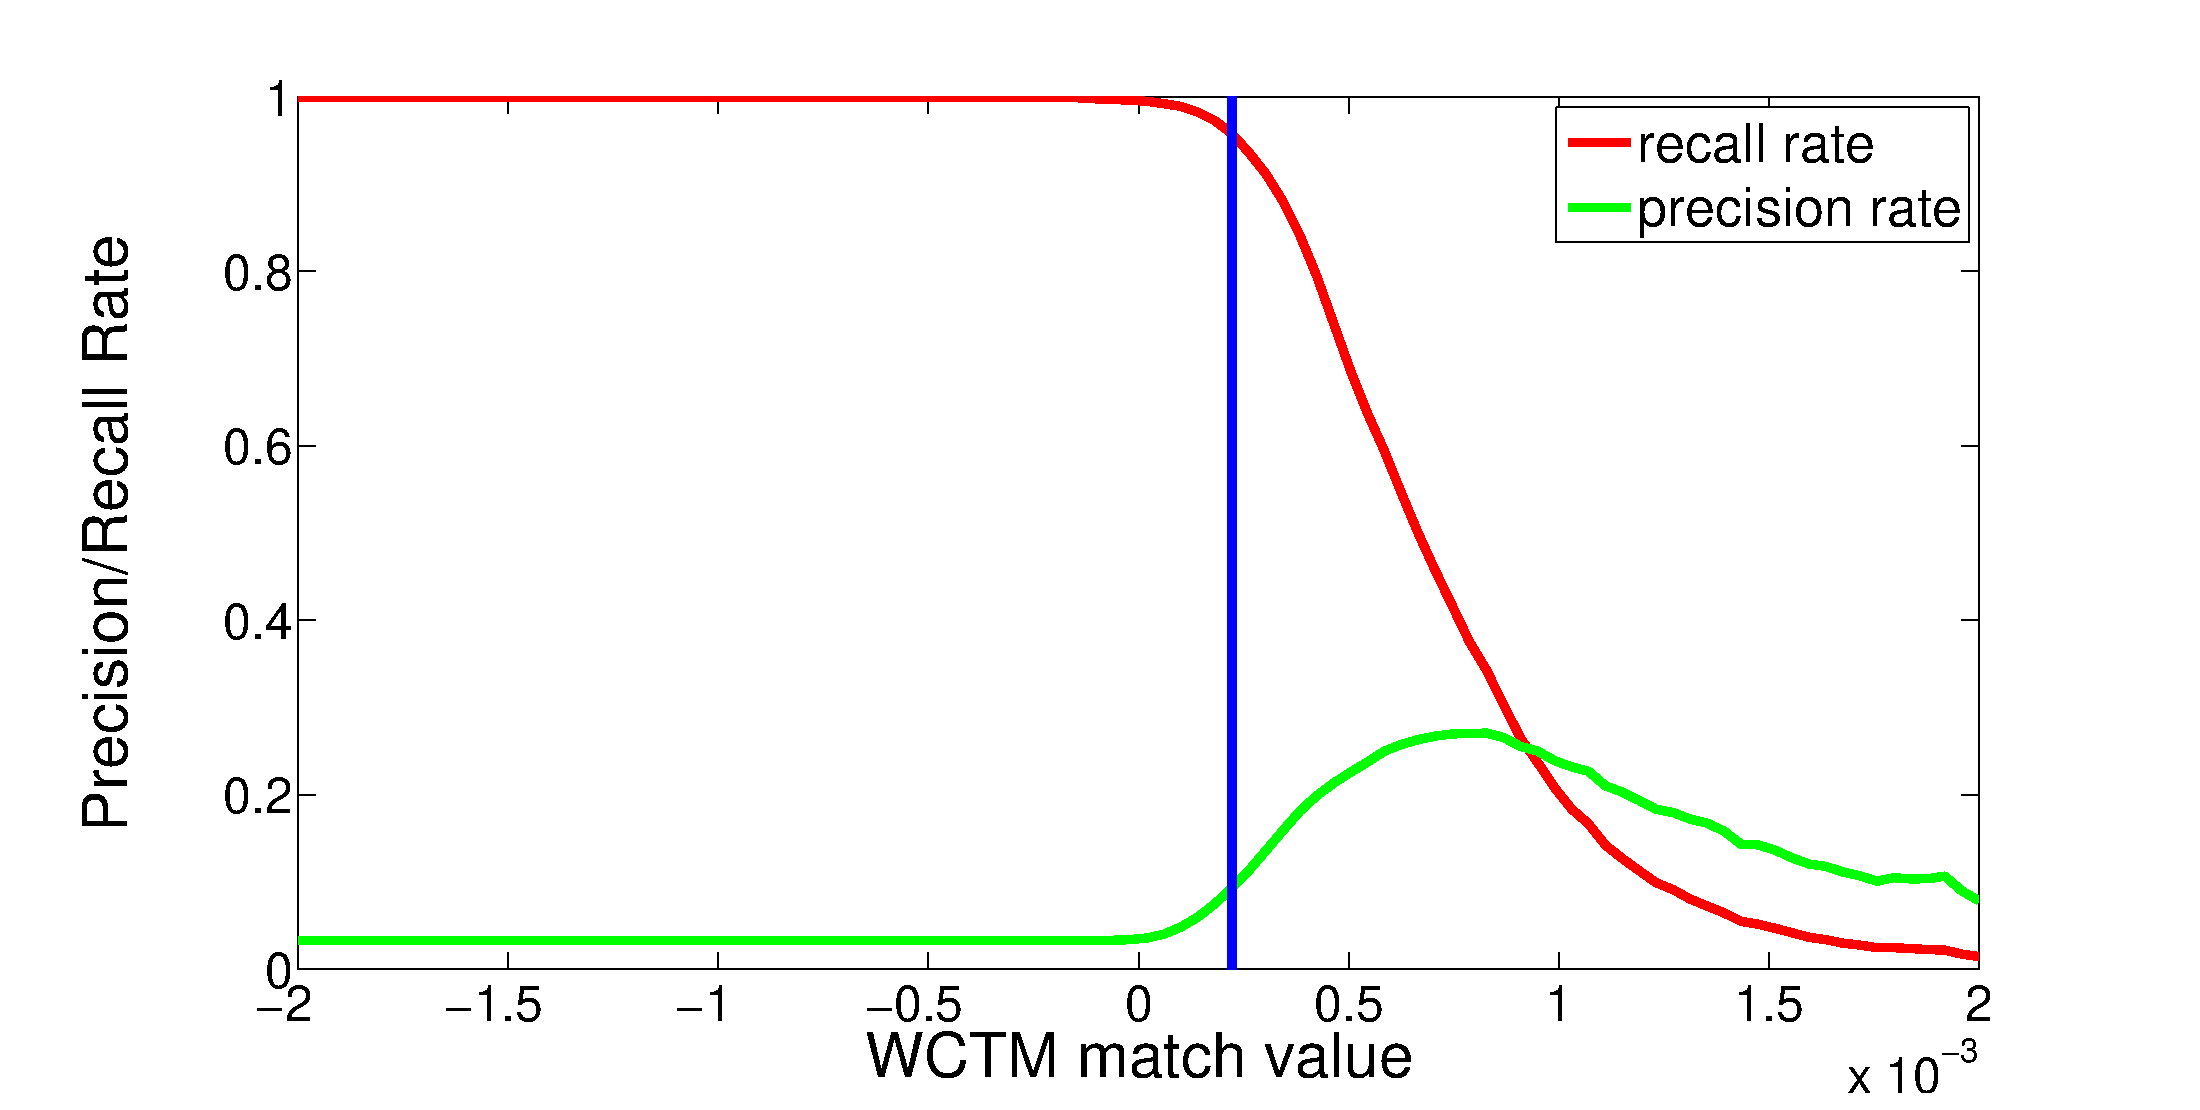
\includegraphics[width=\textwidth]{layer4_precision_recall}
      \caption{}
      \label{subfig:layer4_precision_recall}
  \end{subfigure}
  \begin{subfigure}{0.45\textwidth}
      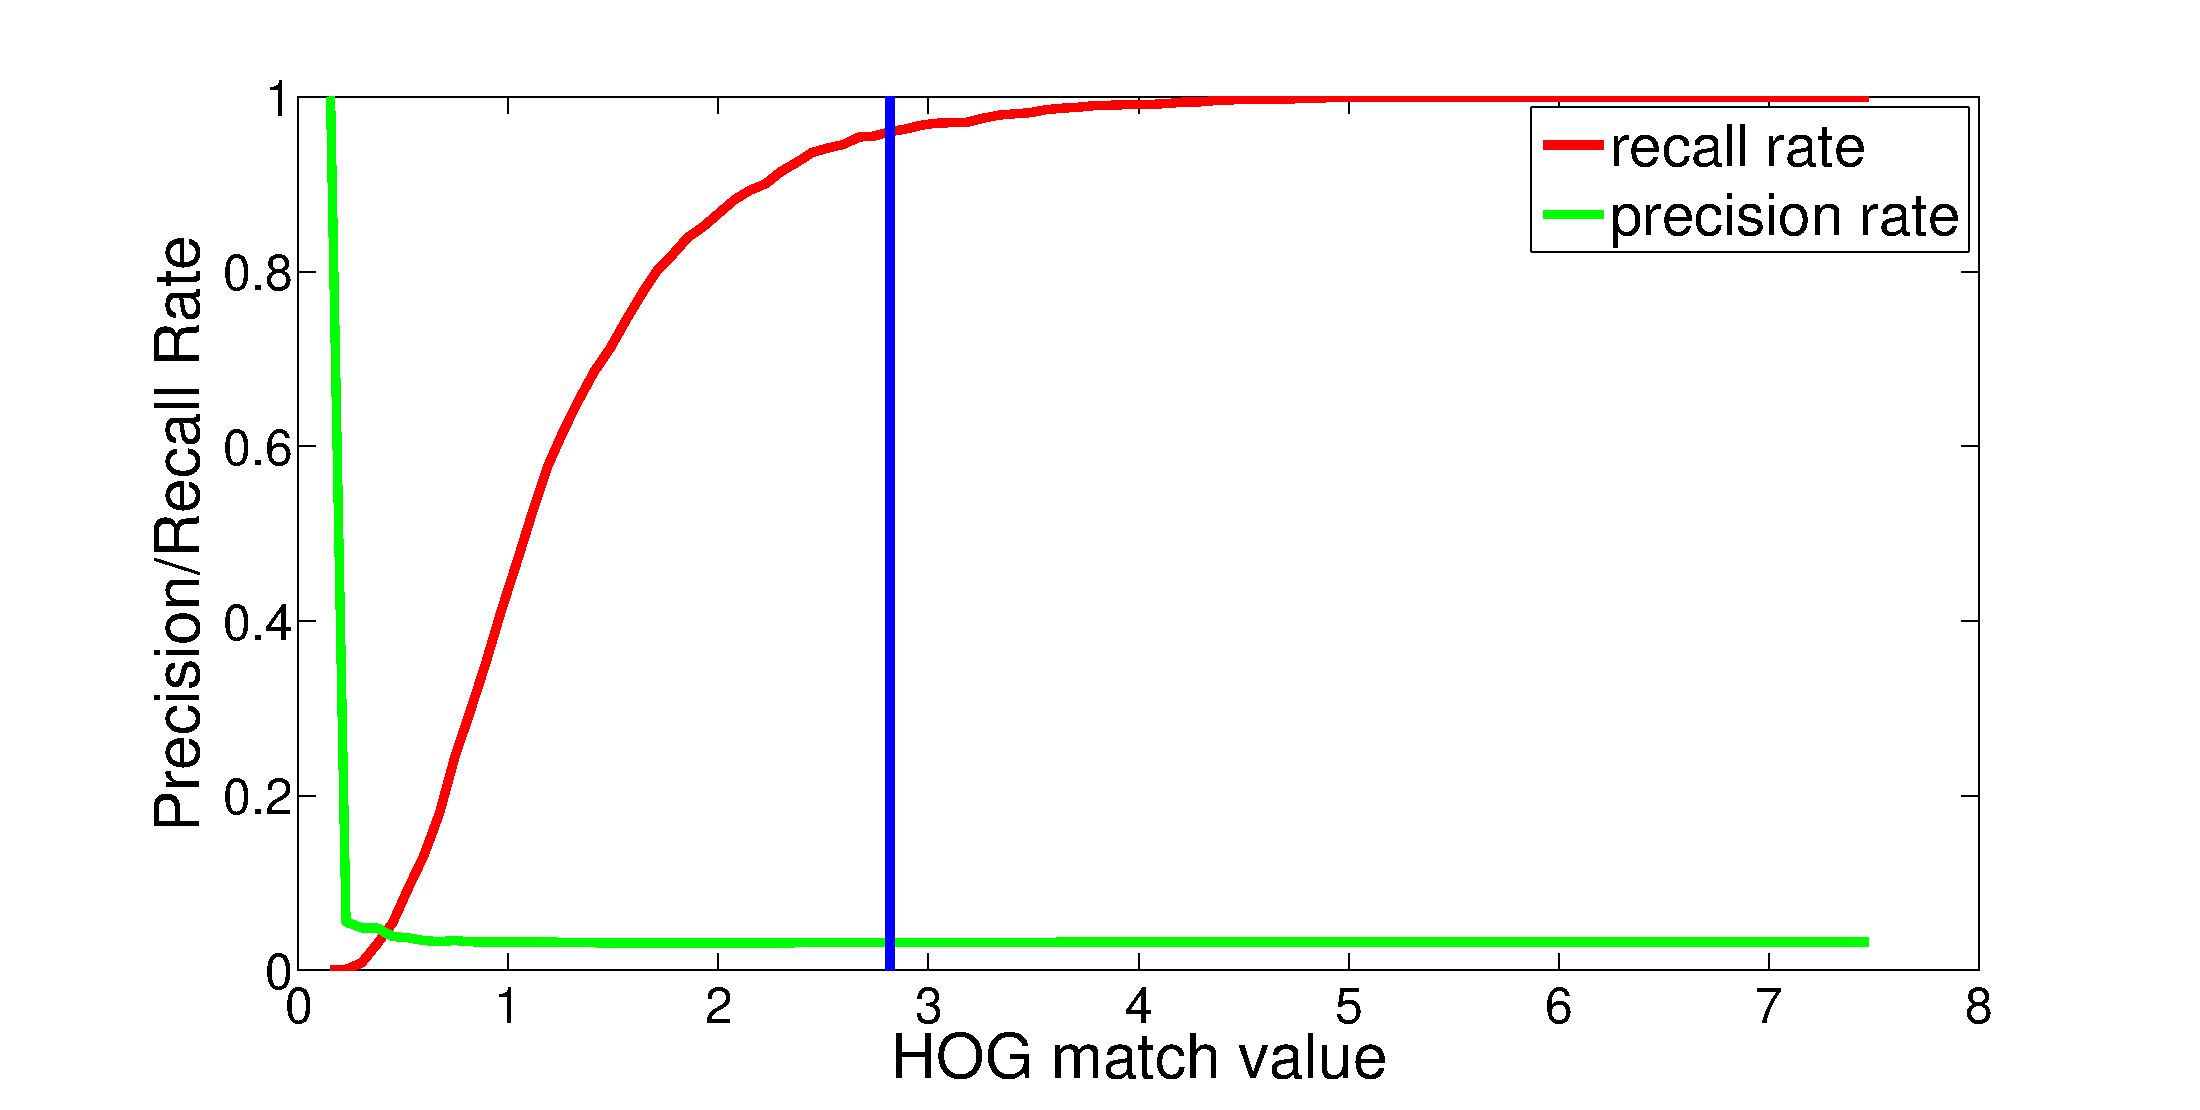
\includegraphics[width=\textwidth]{layer4_hog_precision_recall}       
      \caption{}
      \label{subfig:hog_precision_recall}
  \end{subfigure}
  \caption[Precision-Recall curves for False-positive Filtering Layer]{Precision recall curve for Layer IV candidate methods (a) \gls{wctm} and (b) \gls{hog}. The blue line marks thresholds $D_\mathsf{wctm}=0.0002222$ and $D_\mathsf{hog}=2.816$. It is important to note that \gls{wctm} is a similarity measure and \gls{hog} is a dissimilarity measure. This implies that only instances below the indicated threshold $D_\mathsf{wctm}$ in \gls{wctm}, and likewise instances above the threshold $D_\mathsf{hog}$ in \gls{hog}, are rejected as false positives. }
\end{figure}

\subsubsection{Histogram of Gradients (HOG)}
The \gls{hog} feature descriptor encodes an object by capturing a series of local gradients in neighborhood of the object pixels. 
These gradients are then transformed into a histogram after discretization and normalization. 
There are several variants of \gls{hog} feature descriptors. 
The \textsc{R-}\gls{hog} used for human detection in \cite{dalal} was tested here as a possible Layer IV candidate.

To produce \textsc{R-}\gls{hog}, the image is first tiled into a series of $8\times8$ pixel groups referred to here as cells (the image dimensions need to be multiples of 8). 
The cells are further divided into a series of overlapping blocks each containing groups of $2\times2$ cells. 
For each cell a set of 64 gradient vectors (one per pixel) is computed. 
Each gradient vector contains a direction and magnitude component. 
In the gradient directions, the sign is ignored reducing the range of angles from 0--360 down to 0--180. 
The gradient vectors are then binned into a 9--bin histogram ranging from 0--180 degrees with a bin width of 20 degrees. 
The contribution of each gradient vector is computed as half its gradient magnitude. 
The other half of the gradient magnitude is split between the two neighboring bins (in case of boundary bins, the neighbors are determined by wrapping around the histogram). 
The histograms from the 4 cells in each block is then concatenated to get vector $v$ of $36$ values ($9$ per cell). 
These vectors from each block are then normalized using their $L_2$-norm; for a vector $v$ this normalization would be expressed as
\[
 \bar{v}=\frac{v}{\sqrt{\|v\|^2_2+\epsilon^2}}
\]
where $\epsilon$ is a small constant (here $\epsilon=0.01$). 
The normalized vector $\bar{v}$ from each block is concatenated into a single feature vector $F$ to get the \gls{hog} descriptor for the input image. 
%

Since this method imposes a constraint on the image dimensions being multiples of 8, the learning samples (each cropped using a square window of size of $3\times \text{radius}$) are resized to $24\times24$. 
Here, we have to use both positive and negative object samples, the latter being objects other than scallops picked up in the segmentation layer. 
A \gls{hog} feature vector $F$ of length $144\enspace (4\enspace \text{blocks} \times4\enspace \text{cells} \times9\enspace \text{values})$ is computed for each object instance obtained from the classification layer.

Now several different machine learning methods can be applied, using the positive and negative object instances as learning samples. 
As per the original implementation of the \textsc{R-}\gls{hog} method \cite{dalal}, an \gls{svm} is used here. 
It turns out that the \gls{svm} learning algorithm fails to converge even after a large number of iterations. 
This could be attributed to the fact that the scallop profiles  vary significantly based on their position in the image. 
To overcome this limitation, a lookup table similar to the one used to learn the scallop profiles in the classification layer is generated. 
The only difference here is that instead of saving a reference scallop template vector, a reference \gls{hog} vector for only positive scallop instances from the learning set is recorded. 
The reference \gls{hog} descriptor for a pixel coordinate in the image is taken to be the mean of all the \gls{hog} descriptors of scallop instances inside a $40\times40$ window around the point.

For each instance classified as a scallop from the classification layer, its \gls{hog} descriptor is compared with its corresponding learned reference \gls{hog} descriptor from the lookup table.
Since \gls{hog} feature vectors are essentially histograms, the \gls{emd} metric \cite{rubner} is used to measure the dissimilarity between feature and object histograms.
%Technically, the \gls{emd} quantifies the difference between two histograms. Intuitively, if histogram bins are thought of as containers of dirt with the volume of dirt in each bin is analogous to the bin frequency, then the amount of work done moving piles of dirt to match a different histogram arrangement is equivalent to the \gls{emd}  between the two histograms. 
Let $A$ and $B$ be two histograms, and let $m$ and $n$ be the number of bins in $A$ and $B$, respectively.
Denote $d_{ij}$ the spatial (integer) distance between bin $i$ in $A$ and bin $j$ in $B$, and $f_{ij}$ the smaller number of items that can be moved between bins $i$ and $j$ to ultimately make both histograms match (this is known as the \emph{optimal flow} and can be found through a process of solving a linear program \cite{rubner}).
Then the \gls{emd} metric $D_\mathsf{emd}$ that quantifies dissimilarity between two histograms $A$ and $B$ would be expressed as
%
\[
 D_\mathsf{emd}(A,B)=\frac{\sum_{i=1}^m\sum_{j=1}^nd_{ij}f_{ij}}{\sum_{i=1}^m\sum_{j=1}^nf_{ij}} \enspace.
\]


A precision-recall curve (shown in Figure~\ref{subfig:hog_precision_recall}) with the classification threshold set as $2.816$ (which corresponds to 96\% recall rate, same rate used to set the \gls{wctm} threshold). 
Any object with \gls{emd} distance value less than this threshold is considered as a scallop.
 Though this threshold can capture 96\% of the scallops, very few false positives actually get eliminated (less than 3\%).

%========================================================================================
\section{Results}
%
The multi-layered detection approach is tested on two separate datasets containing  $1\,299$ and $8\,049$ images, respectively.
Among the two candidate methods tested for the fourth layer, \gls{wctm} was chosen over \gls{hog} due to it superior performance in terms of eliminating false positives. 
The difference in performance between \gls{hog} and \gls{wctm} is given in Table~\ref{tab:false_positives} for both datasets. 
Rows 1 and 2 in Table~\ref{tab:false_positives} show the true positives and false positives, respectively, that are filtered down from the initial 3 layers (Layers I-III). 
With these values as baseline, the thresholds for both \gls{hog} and \gls{wctm} were chosen to retain a high recall rate of close to 96\%. 
This ensures that very few true positives are lost and their performance is primarily assessed through the reduction in false positives (row 6 of Table~\ref{tab:false_positives}). 

\begin{table*}
  \centering
  \begin{threeparttable}
    \begin{tabular}{lllll}
\toprule[1pt]
	&\multicolumn{2}{c}{\gls{hog}}	&\multicolumn{2}{c}{\gls{wctm}}\\
	&Dataset 1	&Dataset 2	&Dataset 1	&Dataset 2\\ [2pt]\cline{1-5}\\[-5pt]
TP\tnote{1} ~from Classification Layer	&183		&1\,759		&183		&1759\\
FP\tnote{2} ~from Classification Layer	&7\,970		&52\,456		&7\,970		&52\,456\\
TP after Layer IV 			&179		&1\,689		&176		&1\,685\\
FP after Layer IV 			&7\,752		&51\,329		&2\,924		&16\,407\\
Decrease in TP after Layer IV	&4 (2.2\%)	&70 (4\%)	&7 (3.8\%)	&74(4.2\%)\\
Decrease in FP after Layer IV	&218 (2.7\%)	&1\,127 (2.1\%)	&5\,046 (63.3\%)	&36\,049 (68.7\%)\\ \bottomrule
    \end{tabular}
    \begin{tablenotes}
	  \item[1] \footnotesize{TP--True Positives}
	  \item[2] \footnotesize{FP--False Positives}
    \end{tablenotes}                                                      
  \end{threeparttable}
  \caption{Comparison of tested false positive filter layer methods}
  \label{tab:false_positives}
\end{table*}      
%
Since the thresholds are set such that the recall rate is high in both methods, the decrease in true positives is less than 5\% in both \gls{hog} and \gls{wctm}. 
However there is a significant reduction in false positives (63.3\% for dataset 1 and 68.7\% for dataset 2)  due to \gls{wctm}. 
On the other hand, the decrease in false positives is relatively small (less than 3\%) for \gls{hog}.
It is not clear at this point why the \gls{hog} filter fails to remove  false positives. 
One reason could be that the \gls{hog} filter derived from its native implementation for human detection in \cite{dalal} might need further customization and even weighting through standard deviation weights like in \gls{wctm}. 
Further study and detailed analysis is required to investigate and possibly improve its performance. 
In any case, the results support the inclusion of \gls{wctm} as the false positive filter layer in the multi-layer scallop detection and counting process pipeline.

The overall performance of the four-layer pipeline is shown in Table \ref{tab:count_results}.  
The results are compared to manually labeled ground truth.
Only a subset of the available scallops---scallops at least 80 pixels horizontally and 60 pixels vertically away from the image boundaries---were used as ground truth.
This was done to leave out scallops near the boundaries that were affected by severe vignetting effects. 
Such scallops were often too dark (see Figure~\ref{fig:scallopred}) and very difficult to correct using standard vignetting correction algorithms.
Furthermore, the scallop templates for scallops near the boundaries are such that their prime feature, the dark crescents, blend into the dark borders of the image (see Figure~\ref{subfig:mean_quadrant}). 
Inclusion of the boundaries would cause almost any objects near the boundary to be classified as scallops, resulting in a large number of false positives.
It is also interesting to note that scallops only partially visible near the image boundaries were excluded in the manual counts performed \cite{walker}.

\begin{table*}
\caption{Results of multi-layer scallop classification \label{tab:count_results}}
\begin{center}
\begin{tabular}{lll}
\toprule[1pt]
 & Dataset 1 & Dataset 2\\[2pt]\cline{1-3}\\[-5pt]
Number of images & 1,299 & 8,049\\
Ground Truth Scallops & 363 & 3,698\\
Valid Ground Truth Scallops & 250 & 2,781\\
True positives after Visual Attention Layer & 231 (92.4\%) & 2,397 (86.2\%)\\
True positives after Segmentation Layer & 185 (74\%) & 1,807 (64\%)\\
True positives after Classification Layer & 183 (73\%) & 1,759 (63.2\%)\\
True positives after False Positive Filter Layer & 176 (70.4\%) & 1,685 (60.6\%)\\
False positives after Classification Layer & 7,970 & 52,456\\
False positives after False Positives Filter Layer (\gls{wctm}) & 2,924 & 16,407\\
Decrease in false positives (due to \gls{wctm}) & 63.3\% & 68.7\%\\ \bottomrule
                               \end{tabular}
                               \end{center}
                               \end{table*}      
   
Table \ref{tab:count_results} shows the results of the 3-layer pipeline along with the improvements in terms of the reduction in false positives as a result of introducing the fourth processing layer. 
The true positive percentages shown are computed with reference to the valid ground truth scallops (row 3 of table \ref{tab:count_results}), i.e., scallops away from image boundaries.  
In dataset 1, which contains $1\,299$ images, the four-layer filtering results in a 70.4\% overall recall rate, while in dataset 2 that contains $8\,049$ images the overall recall rate is 60.6\%.  Though the addition of the fourth false positive layer results in a small drop of 2.6\% in recall rate, it eliminates over 63\% of the false positives in both datasets.
There is no clear reason for the better performance of this pipeline on dataset 2 both in terms of recall rate and decrease in false positives compared to dataset 1.

%========================================================================================
\section{Discussion}
\label{sec:scallop_discussion}

The four-layer automated scallop detection approach discussed
here works on feature-poor, low-light imagery and yields
overall detection rates in the range of 60--70\%. 
Related work on scallop detection using underwater imaging \cite{dawkins11,dawkings13},
reported higher detection rates, but the quality of the images used was visibly better.  Specifically,
the datasets on which the 
alternative algorithms \cite{dawkings13}
operated on, exhibit much more uniform lighting conditions, higher resolution,
brightness, contrast, and color variance between scallops and background 
(see Figure~\ref{data-difference}). 
Evidence of this can be seen in Figure~\ref{data-difference}: the color variation between scallops and background data is reflected in the
saturation histogram of Figure~\ref{data-difference}. While the histograms
of scallop regions in the datasets of Table~\ref{tab:count_results} is often 
identical to the global histogram of the image, the histograms of the \gls{whoi} data used by the alternative algorithms \cite{dawkings13} present a bimodal saturation histogram
(Figure \ref{subfig:dawkins_hist}), from which 
foreground and background are easily separable.



\begin{figure*}
  \centering
  \begin{minipage}[c]{\textwidth}
    \centering
    \raisebox{1.5mm}{
    \begin{subfigure}[]{0.3\textwidth}
	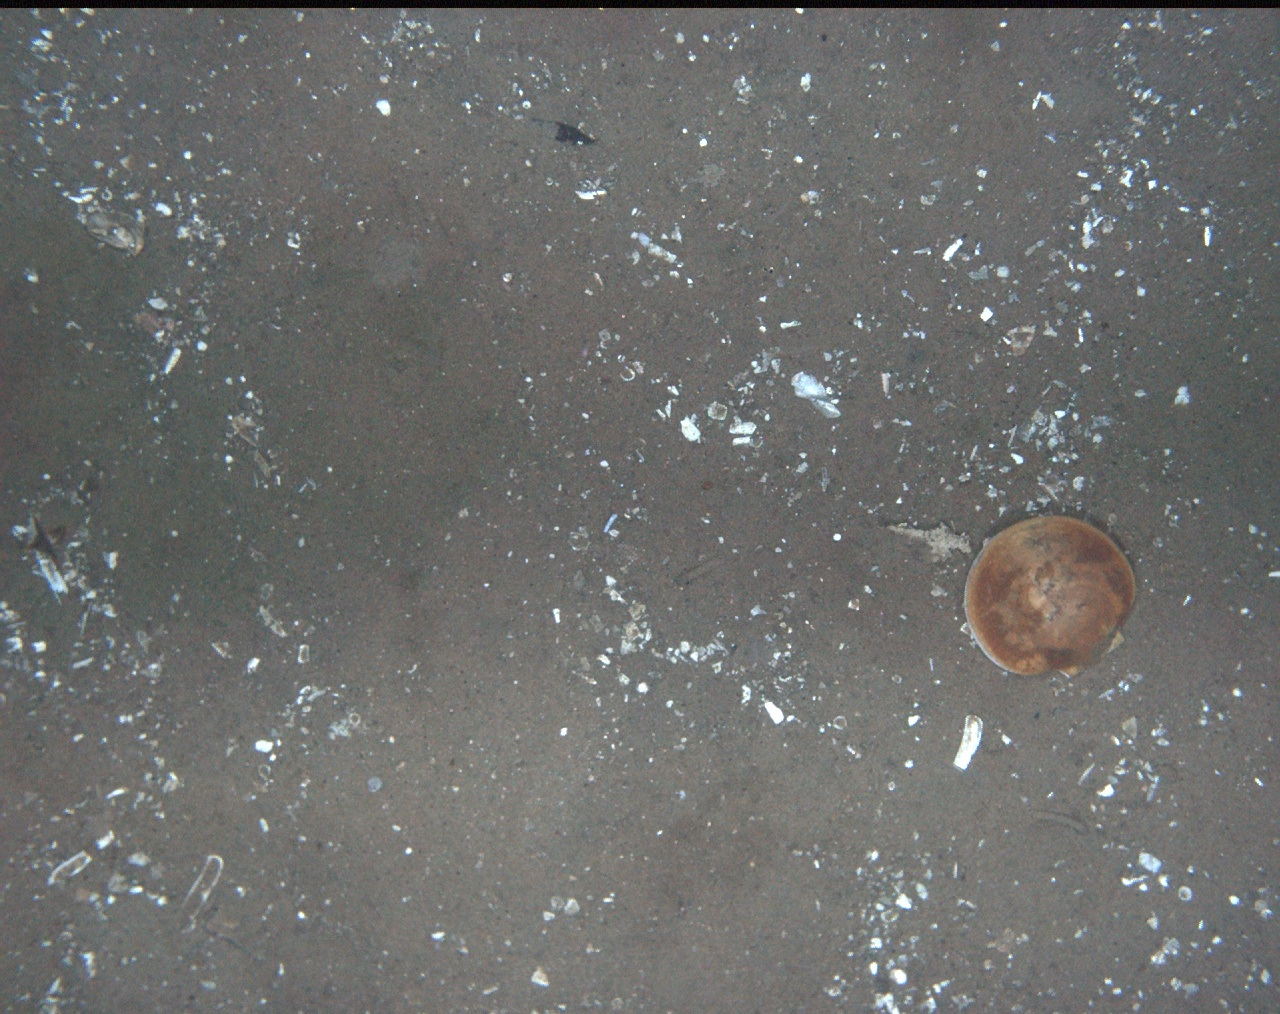
\includegraphics[width=\textwidth,natwidth=1280,natheight=1014]{77616}
	\caption{}
	\label{subfig:dawkins}
    \end{subfigure}
    }
    \begin{subfigure}[]{0.25\textwidth}
	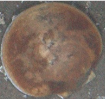
\includegraphics[width=\textwidth,natwidth=105,natheight=100]{dawkins_crop_resize}
	\caption{}
	\label{subfig:dawkins_crop}
	\hskip 15pt
    \end{subfigure}
    \raisebox{2mm}{
    \begin{subfigure}[]{0.33\textwidth}
	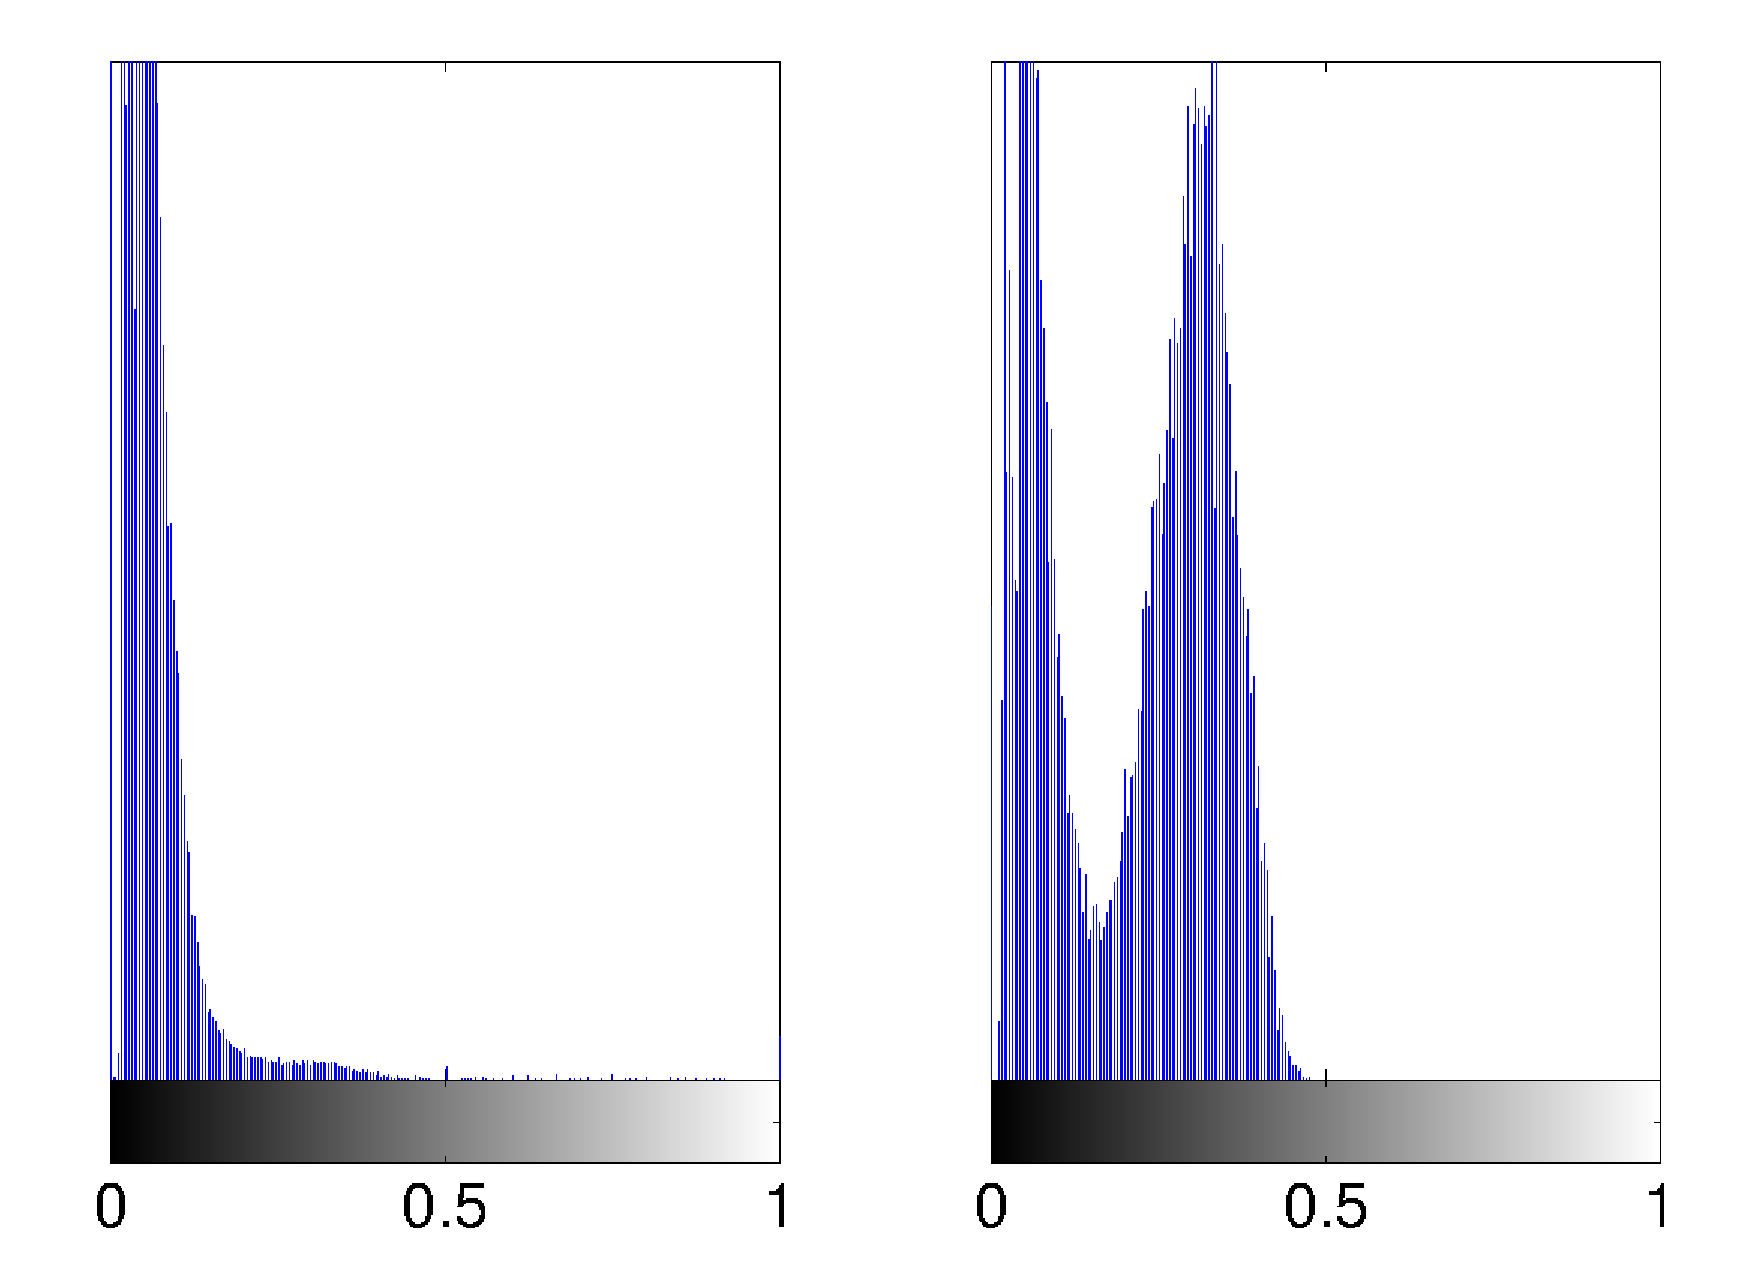
\includegraphics[width=\textwidth]{dawkins_hist_sat}
	\caption{}
	\label{subfig:dawkins_hist}
    \end{subfigure}
    }
  \end{minipage} 

  \vskip 10pt
  \begin{minipage}[c]{\textwidth}
  \centering
    \raisebox{1.5mm}{
    \begin{subfigure}[]{0.32\textwidth}
	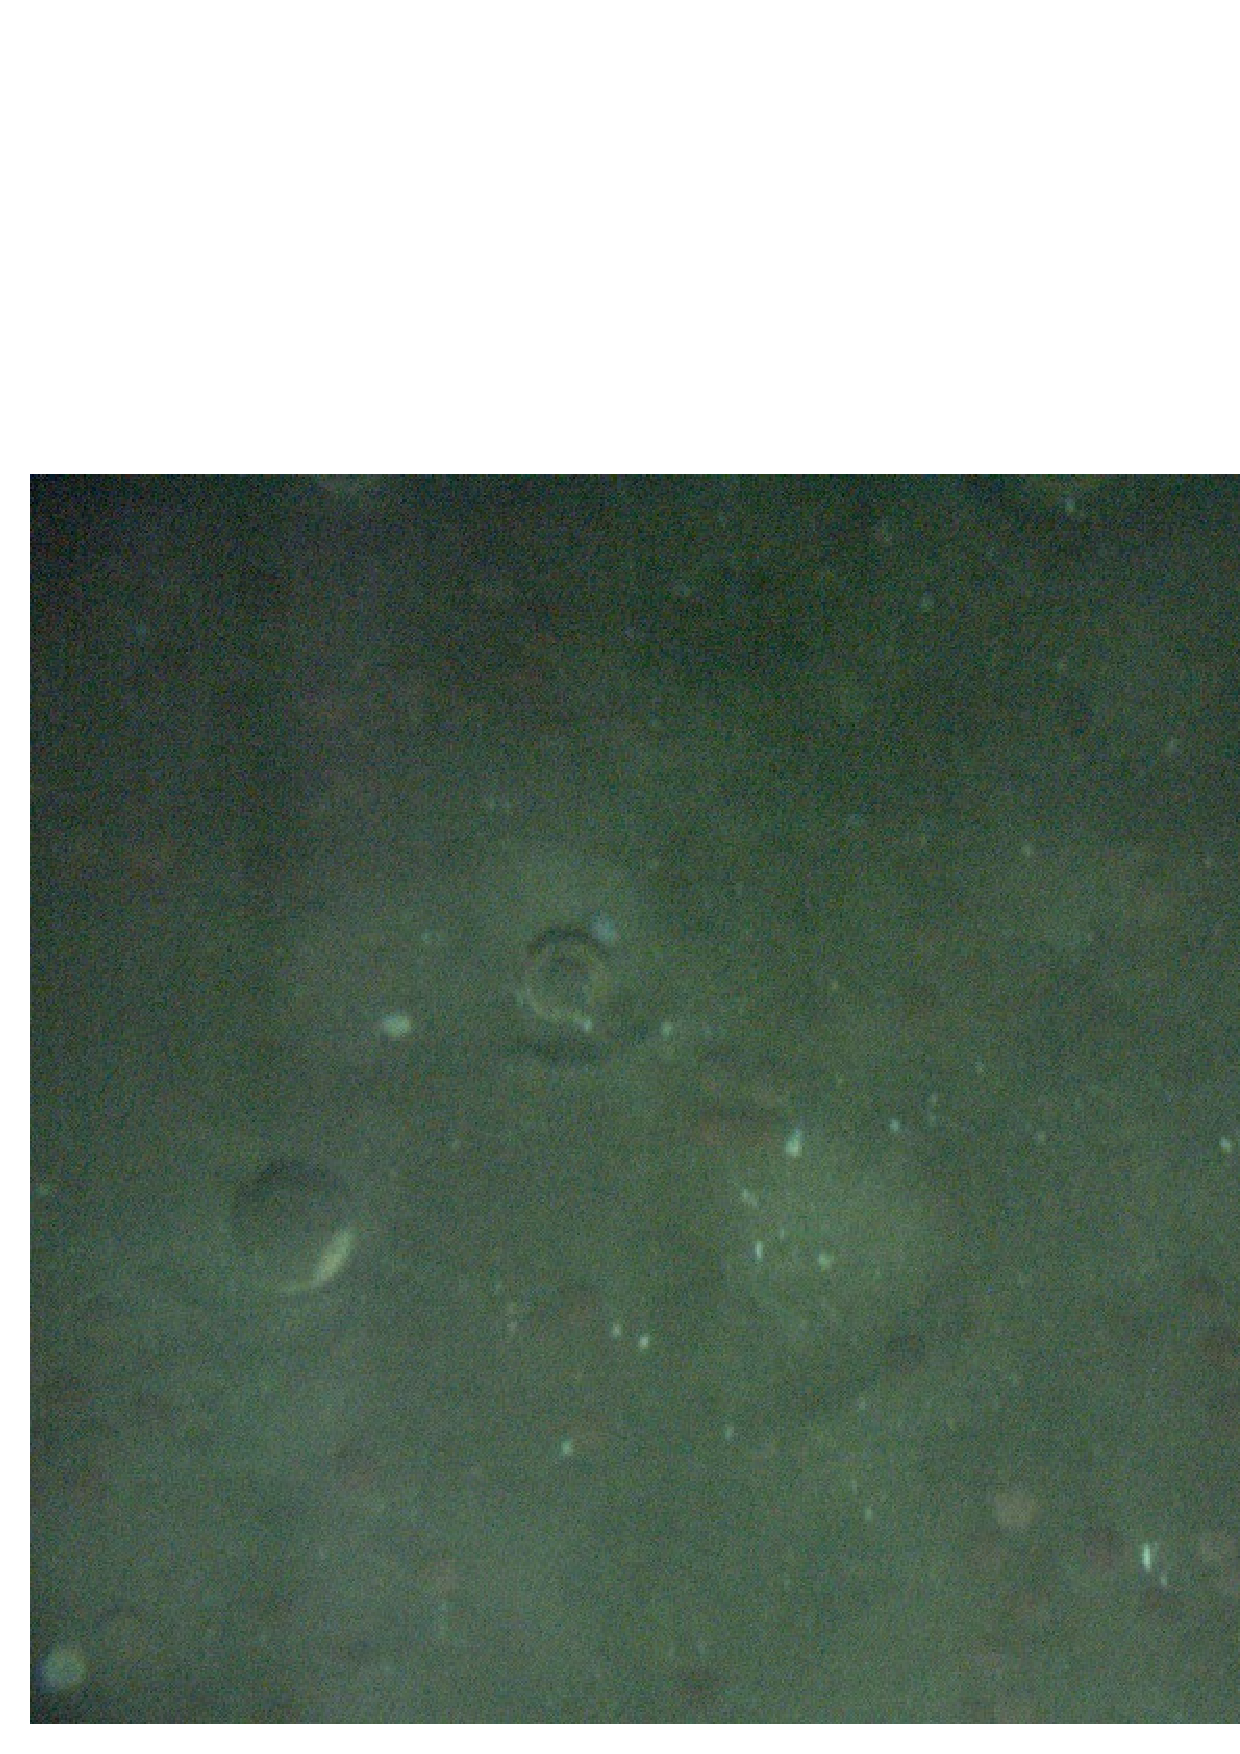
\includegraphics[width=\textwidth]{60} 
  	\caption{}
	\label{subfig:typical}
    \end{subfigure}
    }
    \begin{subfigure}[]{0.235\textwidth}
	
\includegraphics[width=\textwidth]{our_crop_resize}
	\caption{}
	\label{subfig:typical_crop}
	\hskip 15pt
    \end{subfigure}
    \raisebox{2mm}{
    \begin{subfigure}[]{0.35\textwidth}
	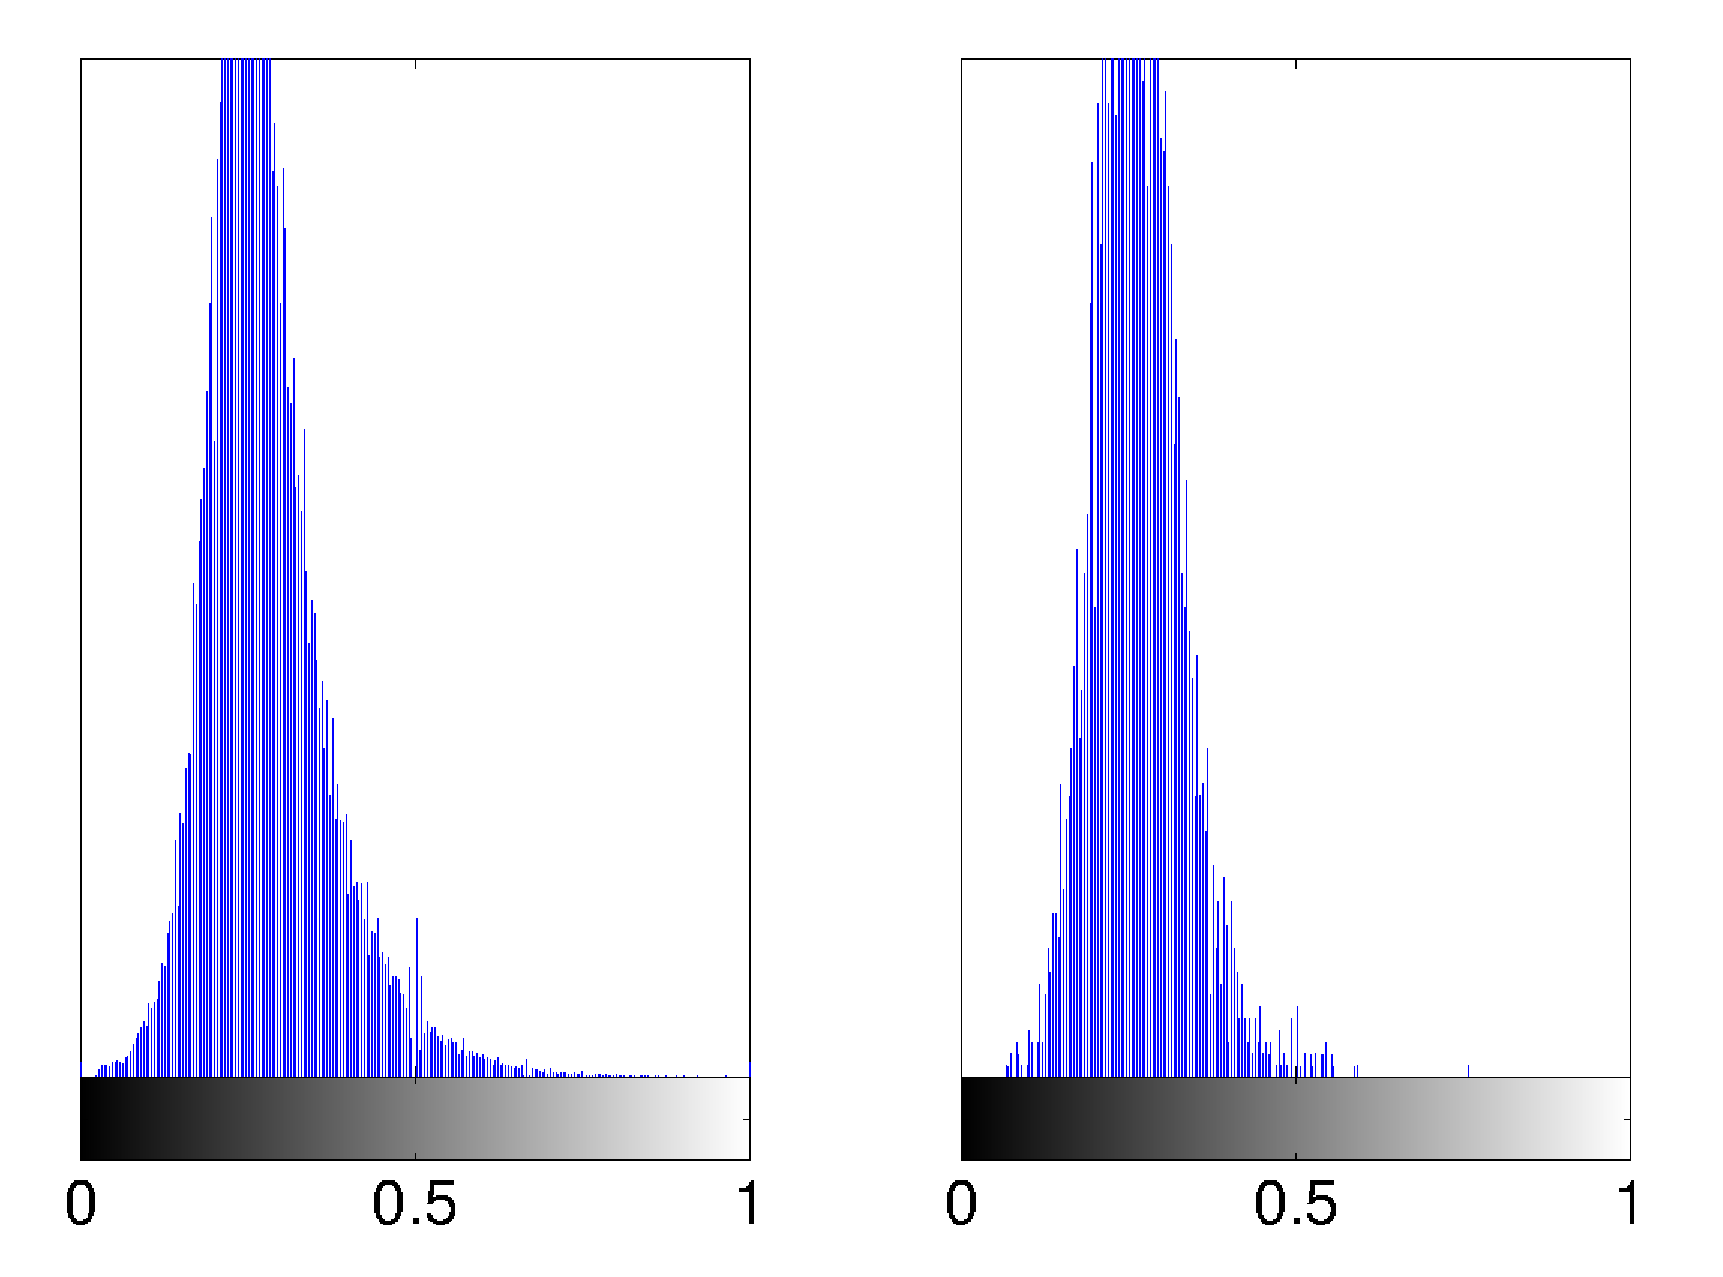
\includegraphics[width=\textwidth]{our_hist_sat}
	\caption{}
	\label{subfig:typical_hist}
    \end{subfigure}
    }
  \end{minipage}
  \caption[Comparison of scallop recognition results with existing methods]{Representative samples of different imagery data on which
  scallop detection algorithms may be called to operate on.  Figures \ref{subfig:dawkins}
  and \ref{subfig:typical},
  show an image containing a single scallop from the dataset used by Dawkins et al.\cite{dawkings13} (used with permission from the authors) 
  and the datasets used in this chapter respectively.
  A magnified
  view of a scallop cropped from Figure \ref{subfig:dawkins} 
  and \ref{subfig:typical} can be seen in Figures \ref{subfig:dawkins_crop} 
  and \ref{subfig:typical_crop} respectively.
  Figure \ref{subfig:dawkins_hist} 
  gives the saturation histogram of background or the complete 
  image in Figure \ref{subfig:dawkins} to left and 
  saturation histogram of Figure \ref{subfig:dawkins_crop} to the right.
  Similarly, Figure \ref{subfig:typical_hist} 
  gives the saturation histogram of Figure \ref{subfig:typical} to the left and 
  saturation histogram of Figure \ref{subfig:typical_crop} to the right. The bimodal 
  nature of the scallop histogram
  in Figure~\ref{subfig:dawkins_hist} 
  derived from the dataset used in Dawkins et al.\cite{dawkings13}, clearly portrays the distinguishing appearance of the scallop pixels from the rest of the image, making it easily identifiable. The datasets we
  used did not exhibit any such characteristics (as seen in Figure~\ref{subfig:typical_hist}) 
  to aid the identification of scallops.}
  \label{data-difference} 
\end{figure*}

Compared to another alternative approach that uses a series of bounding boxes to cover the entire image \cite{guomundsson}, the one reported here employs only ten windows per image, scanning the images at a much faster rate.   
Additionally, the detection rates there \cite{guomundsson} were based on a dataset of just 20 images; statistically significant differences in performance rates between that approach and the one reported here would need much larger image samples.

%========================================================================================
\section{Conclusions}

With the increasing use of underwater robotic platforms, terrabytes of imagery datasets featuring millions of images are becoming commonplace. 
The current practice of manual processing of these underwater images introduces a bottleneck. 
In the spirit of this scallop counting work, designing better and faster automated tools  to characterize animals and other natural underwater phenomenon from images is imperative for future marine environmental studies.

This work is a step toward
the development of an automated procedure for scallop detection, classification
and counting, based on low-resolution imagery data obtained in the organisms' natural environment.
The uniqueness of the reported method lies in its ability to handle poor lighting and low-contrast imaging conditions.
A large natural datasets of over 8000 images have been used to validate this four-layered framework.
Augmenting a previously developed three-layer scallop counting framework with a dedicated false-positive filtering layer has a drastic effect in terms of reducing the number of false positives.
The study noted that a filter based on a custom \gls{wctm} method outperforms \gls{hog} in  this specific application context. 
The multilayer framework reported is verified to be modular, and it allows easy adaptation of different layers for various applications like counting other sea organisms. 
Designing such tools with further improvements in form of higher detection rates and lower false positives is required to help advance future marine animal studies.

%========================================================================================
\section{Future Work}

One future direction would be to further reduce false positives by enhancing the false positives filter layer by using multiple scallop reference templates for each pixel location. 
These new templates could be designed to capture the bright crescents that sometimes appear due to the visible interior of the lower valve of a scallop when the scallop shell is partly open. As this crescent appearance is only dependent on the relative scallop orientation with respect to the camera, it can occur at any point in the periphery of a scallop. If these bright crescents were to be used in conjunction with dark crescents multiple templates will be required to model scallops at each pixel location.
This idea is supported by inspection of recently collected high-resolution scallop data, which indicate additional definitive features connecting the position of the bright and dark crescents along with their relative intensities. 
We believe that even without major changes to the current framework, testing on higher resolution images could produce much better performance outcomes (both in terms of detection and false positive rates). 
The unavailability of ground truth for the new datasets makes it hard to provide evidence of any performance at this point. 
It is also expected that using more targeted color and light correction methods \cite{dawkings13} as a part of image preprocessing will improve results.

Building robust object classification techniques capable of handling noisy data, is one of the primary directions where improvement is necessary. It is possible that a single noisy image of a target object might lack the information needed to accurately recognize it. With this in mind, a multi-view object recognition approach that combines information from multiple images is proposed in Chapter~\ref{chap:distdes}.

%========================================================================================



%=========================================================================================
% Distance Descriptor

\chapter{Distance based Global Descriptors for Multi-view Object Recognition}
\label{chap:distdes}

%================================================================================================================
\section{Introduction}

The ability to recognize objects on distorted images is critical for robotic systems that operate in natural environments where measurement is contaminated by noise. In the presence of noise, the information contained in a single image might not be sufficient to unambiguously classify the \emph{object-of-interest}. This may justify in part the percentage of false positives seen in the multi-layered object recognition approach of Chapter~\ref{chap:scallop_recog}.
One possible way to resolve the ambiguity regarding an object's identity is by combining information from multiple views. The approach described here combines information from multiple views of a target, and employs global image descriptors to solve a classification problem.

Object recognition can be cast as a generalized machine learning problem.
Traditional machine learning approaches \cite{alpaydin} use a learning set with annotated instances to learn the characteristics of an object. A classifier can be used to label a given instance as a target object, if sufficient evidence is available from the learning set to support this hypothesis. Typical machine learning techniques like convolution neural networks \cite{cnn}, use several thousand labeled images to solve the object recognition problem in a purely \emph{data-driven} fashion. In the absence of large labeled datasets for specialized applications like underwater animal recognition, such data-driven approaches require a labor intensive annotation process.

An alternative to a data-driven approach of this type is a \emph{feature-based} object recognition approach \cite{roth}. In feature-based object recognition, prior knowledge about the object to be recognized can be leveraged to build specialized feature descriptors that capture the appearance traits of an object. The models used in such cases can range from simple geometric shapes to complex free-form models \cite{campbell, belongie}. The feature descriptors thus trained encode the object appearance through a low-dimensional mathematical model. This model can be used to check for the presence of an object in an image.

Feature-based approaches can be further subdivided into two classes; local, and global. Local feature-based approaches like the \gls{sift} \cite{sift} and the \gls{surf} \cite{surf} approach, encode a configuration of localized features specific to an object to build a descriptor. In the case of \gls{sift} and \gls{surf}, the feature descriptors obtained are invariant to in-plane rotation and scaling. These properties make \gls{sift} and \gls{surf} very robust and suitable for a multitude of object recognition applications. Since local descriptors primarily depend on artifacts like corners, they are sensitive to noise which degrades and distorts such artifacts. In general, local descriptors can be severely affected by noise in images. On the other hand, global feature descriptors like \textit{gist} \cite{gist} are more resilient to noise, since they encode general characteristics of an image which are less impacted by the presence of noise. Global feature representation also has the additional benefit of not 
requiring segmentation. Segmentation is a hard problem in itself, especially since
it is difficult to delineate foreground and background regions in noisy images. Hence, using a method that does not require segmentation has its benefits. However, the global feature descriptors often only provide a weak description of an object, which might not be sufficient to unambiguously detect its occurrence.

One way to strengthen a weak feature descriptor is to combine information about a single object, derived from multiple information sources. For instance, this can be done by merging information from multiple views of an object. Such an approach is more effective compared to a case in which a single view of an object does not contain sufficient information to unambiguously expose an object. Based on these multiple views, a sequence of hypothesis tests can be combined to eventually classify the object. This process of combining multiple weak classifiers is a common theme in machine learning methods like boosting and bagging \cite{alpaydin}.

The idea of combining multiple sensor measurements is also encountered in the area of active sensing \cite{chen}. In most active sensing problems, for instance in the case of \emph{next best view} \cite{roy,dunn}, the task is to determine successive sensor positions that increase the perceived information  associated with a target object. In the approach described in this chapter, there are differences in the way object classification is ultimately accomplished: a target is observed from several (pre-determined) sensor positions in a way is conceptually similar to active sensing. One difference with active sensing, is that the next sensor position is determined at each iteration based on the current information available.

Combining information from multiple views can also be related to computer vision techniques that operate on the principle of multi-resolution processing or image-pyramid-based methods. Visual attention based object recognition frameworks (like VOCUS \cite{frintrop}), and multi-resolution pedestrian detection \cite{park}, utilize features from multiple scales to build a robust feature descriptor for objects. These multi-resolution techniques essentially resize one image to compute features at different scales. Thus such techniques can only represent the information available from a \emph{single} parent image in different forms. In cases where objects exhibit different appearance traits when viewed from different heights, multiple images of an object are needed to capture \emph{new} information disclosed at different scales.

This chapter describes an object recognition technique that combines information from multiple images of an object gathered from different heights to perform binary classification. The conceptual contribution of this process is in verifying the hypothesis stated earlier regarding the superiority of merging information from multiple views compared to using a single view. The technical contribution is in the design of a novel histogram-based global feature descriptor, along with a hypothesis testing mechanism that combines information from multiple-views of a target object. The approach developed here lies at the intersection of global feature descriptors, active sensing, and multi-resolution image processing to offer a novel object recognition technique that is intended to operate on noisy natural images. The use of global feature descriptors obviates segmentation of noisy images. At the same time, a strong feature descriptor is constructed by combining information from several weak global feature descriptors, each learnt from a different height. This approach also offers a semi-automated annotation framework to minimize the human effort involved in the annotation task.

%================================================================================================================
\section{Preliminaries}

\subsection{Grabcut-in-one-cut Algorithm}
\label{sec:onecut}

A \textit{graphcut} algorithm treats the segmentation problem as a graph partition problem \cite{mincut_maxflow}. Consider a case where each pixel $p$ of an image $I$ is treated as a vertex $i$ in the graph $G(\mathcal{V},\mathcal{N})$. Two neighboring pixels $p$ and $q$, represented by vertices $i$ and $j$ respectively, are connected by an edge $e_{ij}$ in graph $G$. The task of partitioning this graph $G$ into foreground and background is cast as an optimization problem where some form of ``energy'' $E$ is to be minimized. Here, the energy $E$ is formulated as 
%
\begin{equation}	\label{eq:graph_partition}
  E(L)=\sum\limits_{p\in I} D_p(L_p)+\sum\limits_{(p,q)\in \mathcal{N}} V_{p,q} (L_p,L_q)
\end{equation}
%
where $L_p$ corresponds to a labeling for pixel $p$, $D$ is a data penalty function that assigns a likelihood for pixel $p$ to belong to either foreground or background label class, and $V_{p,q}$ is an interaction potential function that encourages spatial coherence by penalizing discontinuity in label values of pixels. A binary partition of this graph is obtained by choosing a label for each pixel $p$ such that the energy $E$ of the image is minimized. This graph-based segmentation approach, also referred to as the max-cut min-flow algorithm was adapted to solve binary image segmentation problems. To this end, a variant called Grabcut-in-one-cut \cite{onecut} uses pre-specified foreground and background seeds to perform a binary partition of an image. According to the Grabcut-in-one-cut algorithm, the energy function in \eqref{eq:graph_partition} is reformed as
%
\begin{equation} \label{eq:graph_partition_onecut}
  E_{seeds}(S)=-\beta \| \theta^S-\theta^{\bar{S}} \|_{L_1}+\lambda|\partial S|\enspace.
\end{equation}
%
Here, $\theta^S$ and $\theta^{\bar{S}}$ are the histograms of the foreground and background pixels in the image. The first term 
of \eqref{eq:graph_partition_onecut}, $\| \theta^S-\theta^{\bar{S}} \|_{L_1}$, penalizes the pixels with intensities that overlap with both foreground and background distributions. The second term of \eqref{eq:graph_partition_onecut}, $|\partial S|$, is a term analogous to $V$ in \eqref{eq:graph_partition}, that tries to enforce similar labeling of neighboring pixels and therefore penalizes a change in labeling across neighbors. The weights $\lambda$ and $\beta$ allow to vary the contribution of the first and second term to the value of the energy function in \eqref{eq:graph_partition_onecut}. Finally, $L_1$ in \eqref{eq:graph_partition_onecut} refers to the $L_1$-norm.

The Grabcut-in-one-cut algorithm generates a binary partition of an image into background and foreground by extrapolating the input foreground and background seed pixels. If there is an automated means to find the location of foreground objects, the seeds required by this algorithm can be automatically generated, hence making this guided segmentation approach fully autonomous.

\subsection{Data Collection Apparatus}

%======================================================================================================
\subsubsection{Imaging Rig}
\label{sec:imaging_rig}

The imaging rig shown in Figure~\ref{fig:im_rig} allows a camera to be held at different heights from the ground for imaging experiments. The height bar slides up or down and can be locked at a specific configuration through specially designed clamps on the scaffold support of the imaging rig. By varying the position of the height bar, the height of the camera holder that is attached to the lower end of the height bar can be varied. This allows the camera held on to the camera holder to capture images of targets placed on the ground from different controlled heights. The camera holder was designed to hold a GoPro Hero 4 camera \cite{gopro}.
	
\begin{figure*}
  \centering
  \begin{subfigure}[]{0.45\textwidth}
      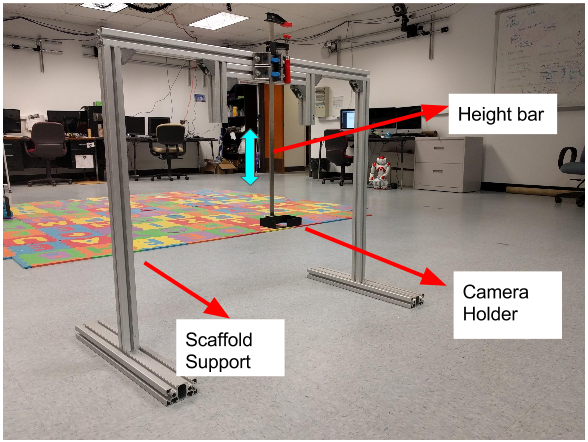
\includegraphics[width=\textwidth]{imaging_rig_labeled}
      \caption{}
      \label{fig:im_rig_side}
  \end{subfigure}
  \begin{subfigure}[]{0.45\textwidth}
      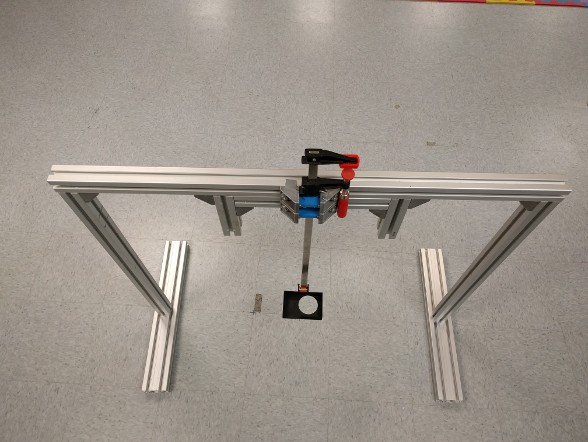
\includegraphics[width=\textwidth]{imaging_rig_top_scaled}
      \caption{}
      \label{fig:im_rig_top}
  \end{subfigure}
\caption[Imaging rig used for data collection in multi-image object recognition approach]{The imaging rig allows the height bar to slide up or down, thereby letting the height of the camera from the ground to be varied. The different components of the imaging rig are labeled in (\subref{fig:im_rig_side}). The camera holder attached to the lower end of the height bar is designed to carry a GoPro Hero 4 camera.}
\label{fig:im_rig}
\end{figure*}	

%======================================================================================================
\subsubsection{Imaging Environment}


The environment where object recognition experiments are performed could affect the performance of the algorithm used. In case of an environment with limited to no control over the imaging parameters, the level of noise introduced into the sensor measurements is difficult to gauge. This complicates the task of designing noise filters to take corrective measures. It might be tempting to perform object recognition experiments in controlled laboratory conditions, where the environmental parameters can be tuned to enhance the performance of an algorithm. However, if an algorithm is intended to operate on natural images, unpredictable variations in environmental factors that could adversely affect the performance of the algorithm are common. To accurately validate an algorithm that is intended to operate on natural environments, it is imperative to choose a 
test environment where the conditions are close to the expected natural conditions. Following this line of reasoning, an underwater environment with uncontrolled lighting was chosen as the test environment--since this object recognition algorithm is intended to operate on noisy natural environments. A circular tank in the Robot Discovery Lab (RDL) at University of Delaware filled with 4 feet of fresh water was thus utilized to collect experimental data. The imaging rig described in Section~\ref{sec:imaging_rig} was submerged inside this test tank during the data collection process.

%======================================================================================================
\subsubsection{Object Specimens}


The focus of this work is to recognize a class of objects that can exhibit some level of intra-class variance that is characteristic to naturally occurring objects. One such example is underwater marine organisms, where each species can have several identifiers that distinguish them from a different species. However in most cases, the members of a single species also exhibit some level of variation in their appearance. To accommodate such cases, the specimens used to validate this multi-view object recognition algorithm were required to have \begin{enumerate*}[label=(\roman*)]  \item some characteristics that are unique to the class they belong to, \item small variations with regards to appearance within the same class of objects, and \item easy accessibility for experimentation purposes. \end{enumerate*} All these points were satisfied by natural produce like potatoes, oranges, tomatillos and strawberries. Natural produce exhibit significant inter-class variance, sufficient intra-class variance and are 
readily 
available commercially making them ideal 
candidates for object specimens. Figure~\ref{fig:produce_species} shows an assortment of potatoes and tomatillos to visually reinforce the inter-class and intra-class variance exhibited by naturally occurring objects. The underwater data on which this multi-view algorithm is validated is composed of a set of 11 oranges and 11 strawberries.
%
\begin{figure*}
  \centering
  \begin{subfigure}[]{0.45\textwidth}
      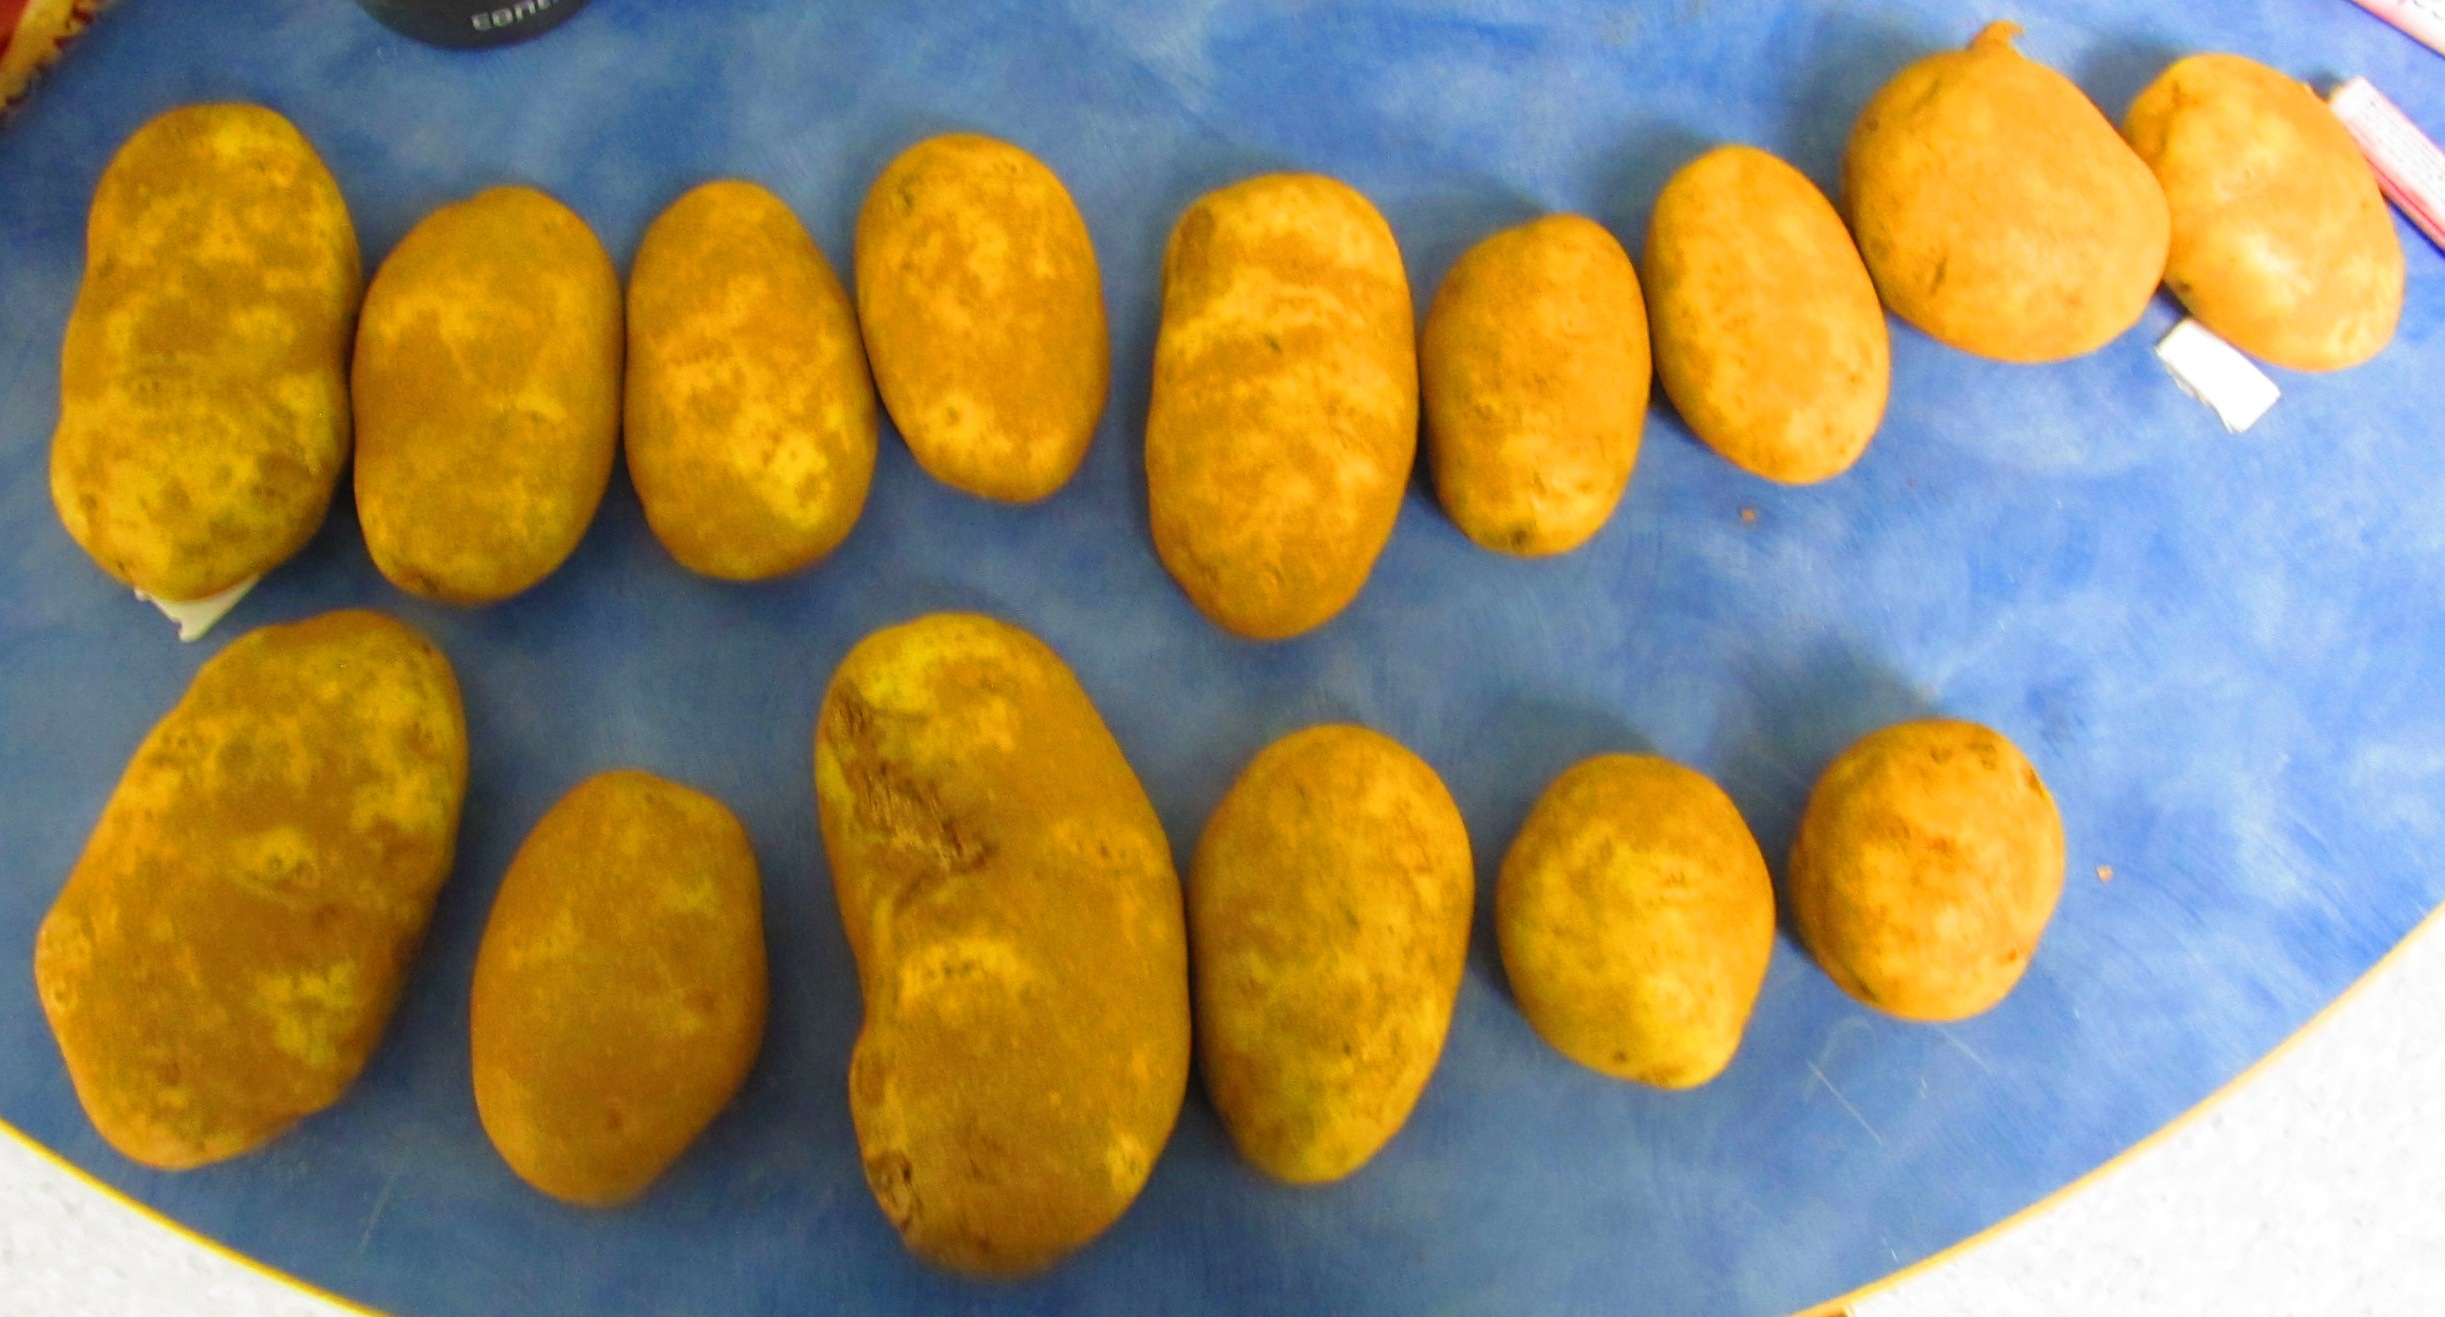
\includegraphics[width=\textwidth]{potatoes_species}
      \caption{Potatoes}
      \label{fig:potato_species}
  \end{subfigure}
  \begin{subfigure}[]{0.45\textwidth}
      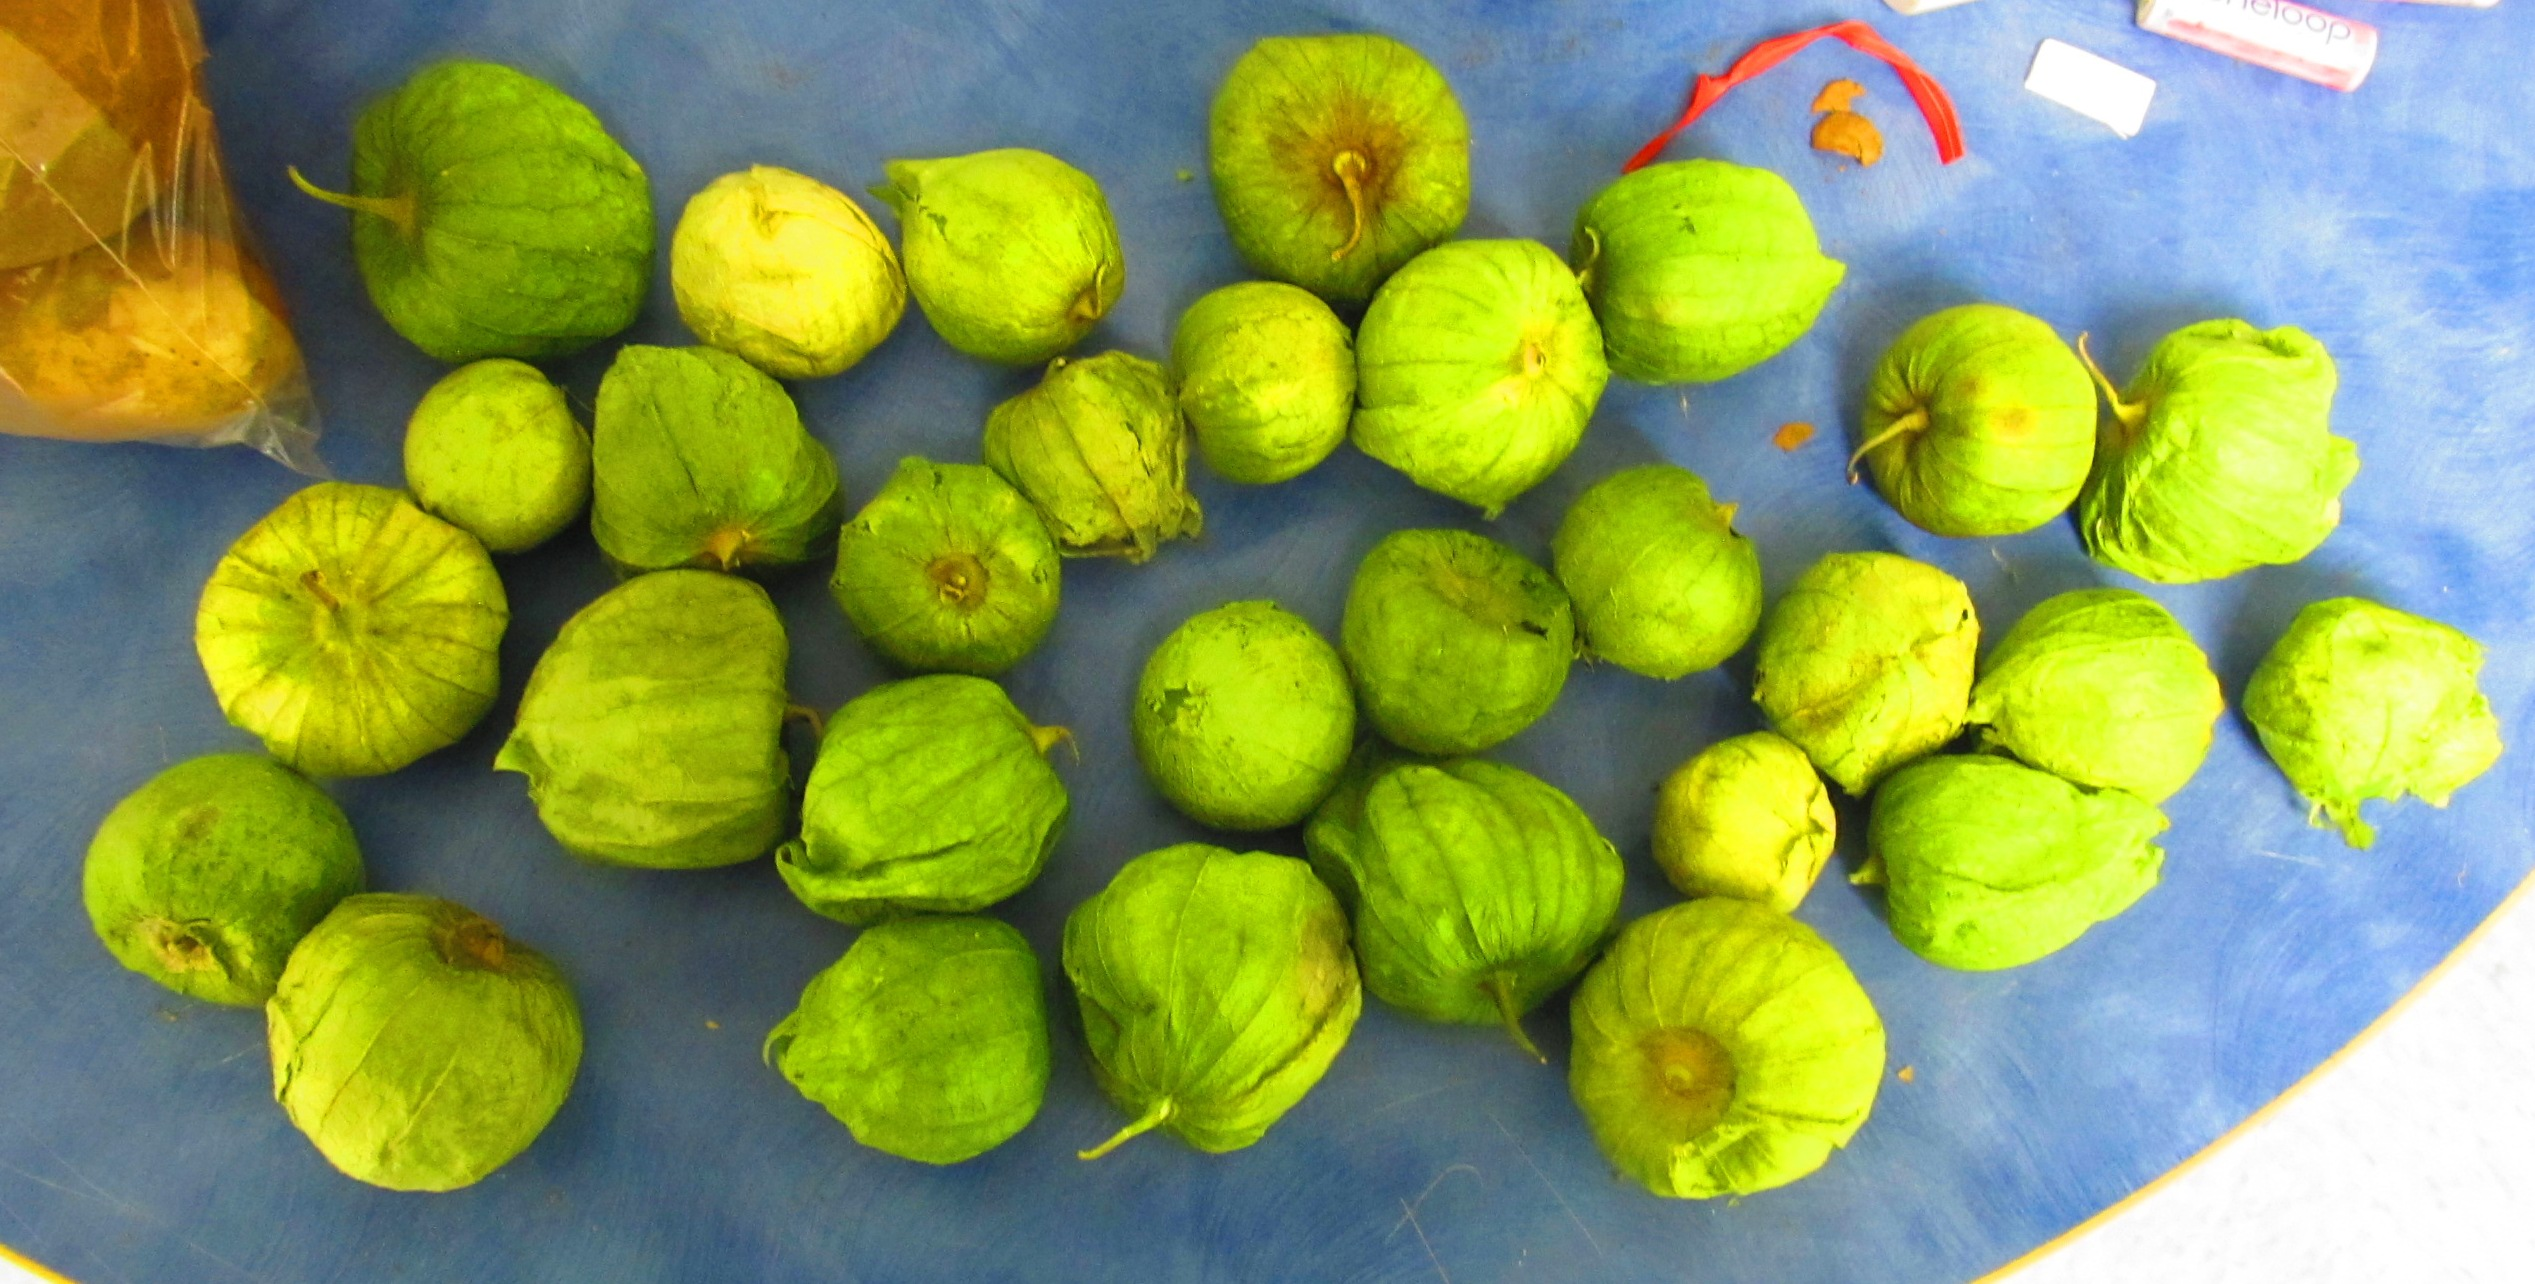
\includegraphics[width=\textwidth]{tomatillos_species}
      \caption{Tomatillos}
      \label{fig:tomatillo_species}
  \end{subfigure}
\caption[Illustration of the inter-class and intra-class variance exhibited by naturally occurring objects]
{An illustration of the inter-class and intra-class variance exhibited by naturally occurring objects like 
potatoes (\subref{fig:potato_species}) and tomatillos (\subref{fig:tomatillo_species})}.
\label{fig:produce_species}
\end{figure*}	
%
%================================================================================================================
\section{Definitions}

\subsection{Histogram Signature}
\label{sec:hist_signature}

As a part of this object recognition technique we define a histogram signature that improves on the generic histogram, specifically designed to deal with possible noise in the pixel values. The rest of this section defines this histogram signature.

A generic histogram $H_f:b_i\mapsto n_i$ of some colorspace $f$, captures the distribution of values of pixels in colorspace $f$, where $n_i$ represents the count of bin $b_i \in \mathcal{B}$, and $\mathcal{B}$ is the set of bins used to partition colorspace $f$. Any pixels affected by noise in image $I$ could corrupt the histogram $H_f$. If we assume that $e\%$ of the pixel values of an image constitutes noise, then the histogram $H_f$ can be refined by rejecting bins containing $e\%$ of pixel values that are least likely to occur according to histogram $H_f$. Before computing the refined version of this histogram, the histogram $H_f$ is first normalized into the form $\bar{H}_f:b_i\mapsto \bar{n}_i$ where
%
\begin{align}	\label{eqn:hist_norm}
 \bar{H}_f(b_i)=\frac{n_i}{\sum_{j}n_j}=\bar{n}_i \enspace.
\end{align}
Now the refined \emph{histogram signature} $\mathcal{H}_f:b_i\mapsto n'_i$ is computed, such that
\begin{align}
  n'_i = 
  \begin{cases}
     \bar{n}_i & b_i \in \bar{\mathcal{B}}_e\\
     0	&	b_i \in \mathcal{B}_e
  \end{cases},
\end{align}
%
where $\mathcal{B}_e$ and $\bar{\mathcal{B}}_e$ constitute a binary partition of $\mathcal{B}$, 
i.e. $\mathcal{B}_e \cap \bar{\mathcal{B}}_e = \varnothing \text{ and } 
\mathcal{B}_e \cup \bar{\mathcal{B}}_e = \mathcal{B}$,
chosen in a way that 
$\bar{\mathcal{B}}_e$ is the smallest cardinality subset of 
$\mathcal{B}$ that satisfies the condition $\sum_{b_i \in \bar{\mathcal{B}}_e} \bar{H}_f(b_i) > 1-e$. 
The definition of set $\bar{\mathcal{B}}_e\subseteq\mathcal{B}$ can be restated as
\begin{align}
 \bar{\mathcal{B}}_e \coloneqq \underset{|\bar{\mathcal{B}_e}|} {\mathrm{argmin}} \sum_{b_i \in \bar{\mathcal{B}_e}} \bar{H}_f(b_i) > 1-e
\end{align}

The $|\mathcal{B}|$-element histogram signature $\mathcal{H}_f$ now encodes the histogram information while attempting to filter some of the noise present in sensor measurements.

\section{Methodology}
\label{sec:distdes_methodology}


The distance-based global descriptor algorithm presented in this chapter is essentially a machine learning technique. As it is common with such techniques, it consists of two parts: a learning part and a validation part. In the learning phase, features and other attributes of an object class are captured from labeled instances of the object available in the learning set. In the validation phase, the learned descriptor for an object class is validated against pre-labeled images to evaluate the performance of an algorithm. The data collection and annotation phases that provide data used for learning and validation parts of this algorithm are discussed next.

\subsection{Data Collection}
\label{sec:distdes_data_collection}



The data collection process here involves capturing images from $t$ different heights for each object specimen. For the validation of this multi-view object recognition algorithm, data was gathered from 22 specimens (11 oranges and 11 strawberries). Each specimen was first placed on the floor below the camera-holder on the imaging rig (see Figure~\ref{fig:im_rig}). The height bar was positioned such that the camera holder was at a distance $d_{max}$ away from the ground. A GoPro Hero 4 camera, attached to the holder, was then triggered to capture an image of the specimen. This first image captured the visual appearance of the specimen while it was at a distance $d_{max}$ away from the ground. After the first image was captured, and without disturbing the object, the next image was captured after bringing the height bar closer to the ground by a distance $d_{step}$.
This process of lowering the camera by distance $d_{step}$ between subsequent images is continued till the camera is no closer than a distance $d_{min}$ from the ground. 
The series of images captured between heights $d_{max}$ and $d_{min}$, with a step-change of distance $d_{step}$ between subsequent images results in $t$ images per specimen, where
\begin{align}
 t=\left\lfloor\frac{d_{max}-d_{min}}{d_{step}}\right\rfloor \enspace. 
\end{align}

Based on restrictions imposed by the imaging rig, the value of parameters for this particular experimental study were set to $d_{max}=32$, $d_{min}=10$ and $d_{step}=2$ (all values in inches).
For example, the design of the imaging rig allowed the camera holder to be set at a maximum distance of $32$ inches from the ground, hence $d_{max}=32$. Furthermore, while testing the imaging rig, it was also found that images captured from any height less than $10$ inches from the ground were subject to significant distortion due to the camera's shadow. To avoid any such distortion, the minimum height was set as $d_{min}=10$. Based on values of $d_{max}$, $d_{min}$ and $d_{step}$, the number of heights per specimen $t=12$ is determined.
These $t$ images capture the appearance of a specimen at different heights. An illustration of the 12 images captured for a strawberry and orange specimen is given in Figure~\ref{fig:height_specimen}. An important point to make here is that the imaging rig is handled manually between each image capture which sometimes results in displacement of the imaging rig or the specimen. 
Additional disturbances in the underwater testing environment where the specimen was placed, sometimes leads to the specimen or the imaging rig getting displaced during the data collection process. These uncontrolled factors in the data collection process added some level of variance to the gathered dataset.
Since this algorithm is intended to operate on uncontrolled natural environments, such variance in the collected data was welcomed to some degree, given that it could test the algorithm's robustness.

\begin{figure*}
  \centering
  \begin{subfigure}[]{\textwidth}
      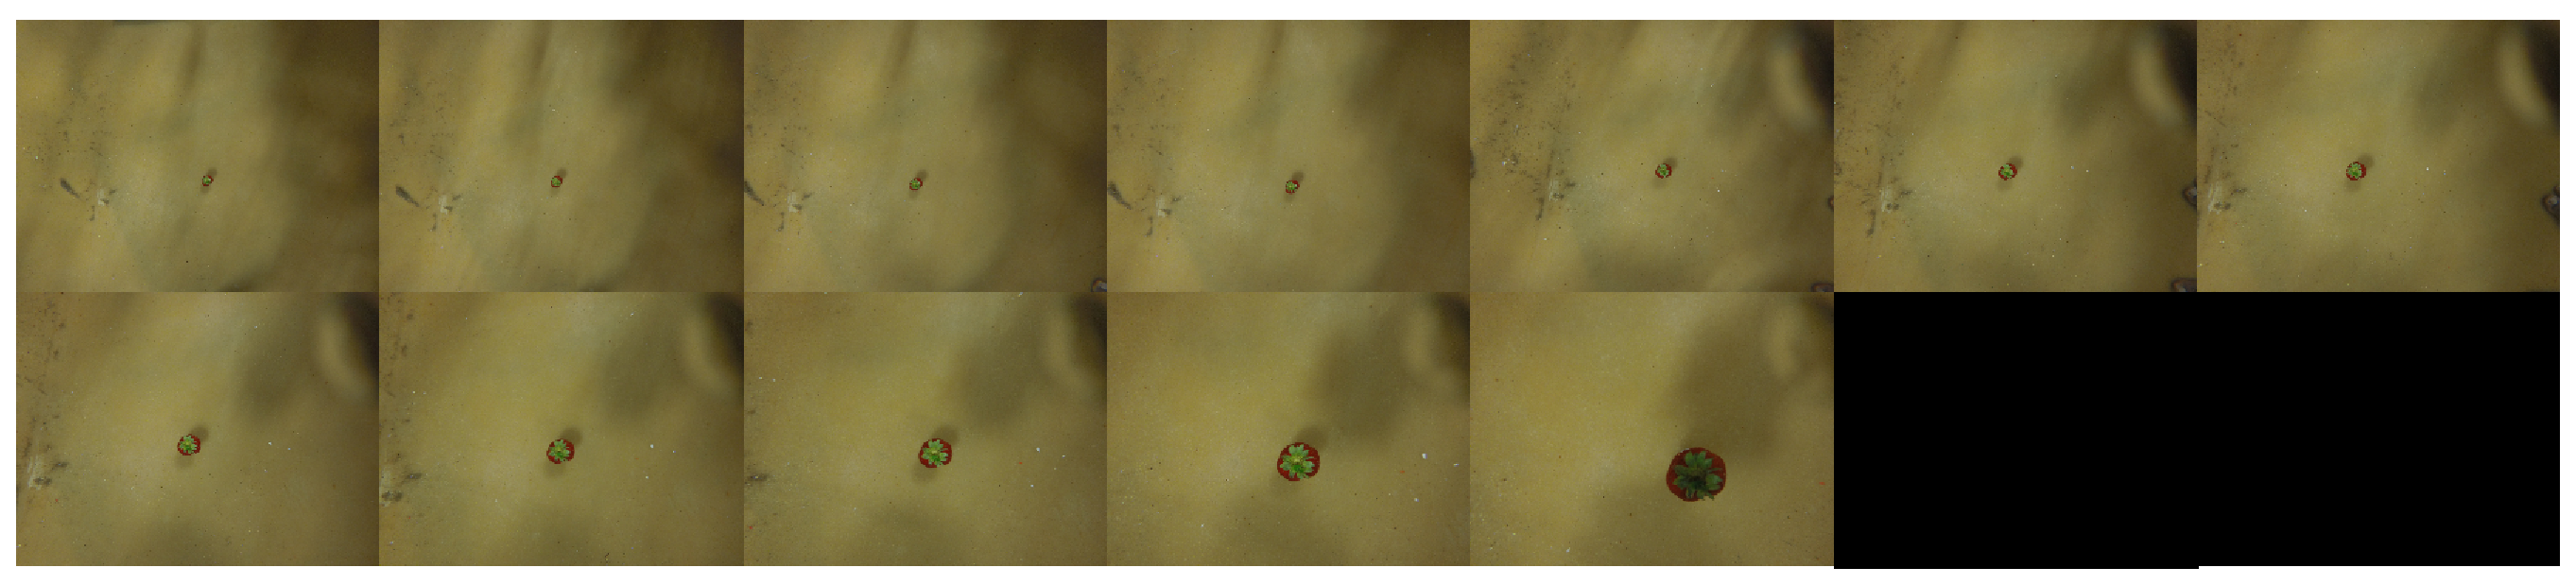
\includegraphics[width=\textwidth]{strawberry_distance_montage_12.eps}
      \caption{Strawberry specimen seen from different heights}
      \label{fig:strawberry_height_specimen}
  \end{subfigure}
  \begin{subfigure}[]{\textwidth}
      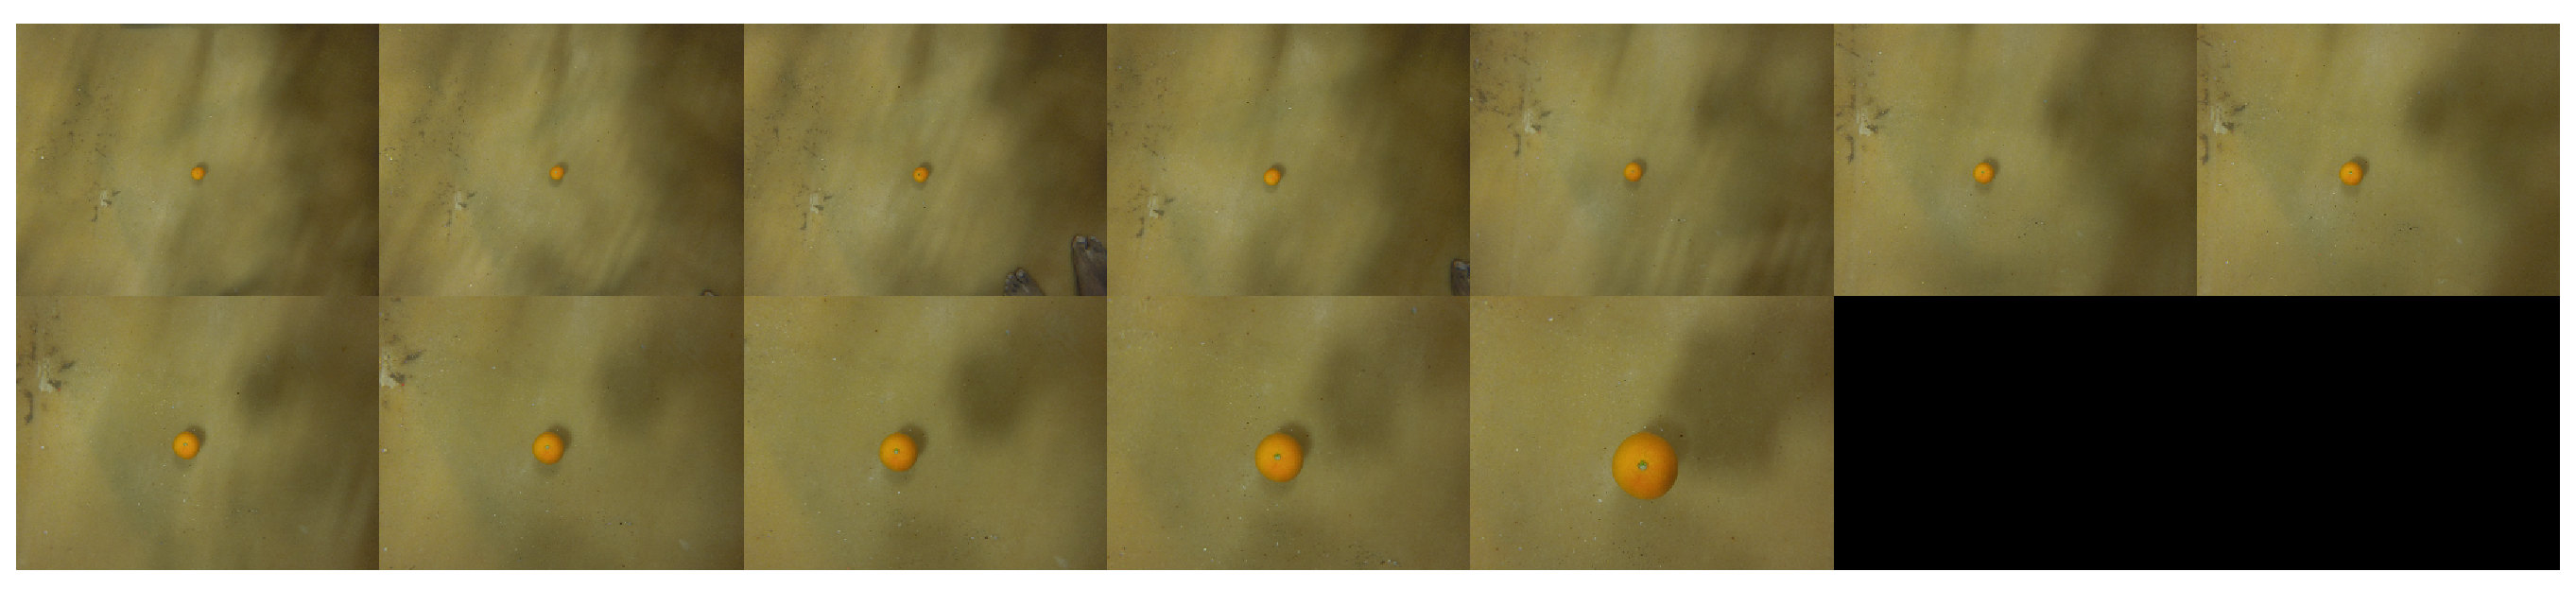
\includegraphics[width=\textwidth]{orange_distance_montage_12.eps}
      \caption{Orange specimen seen from different heights}
      \label{fig:orange_height_specimen}
  \end{subfigure}
\caption[Set of images collected for each specimen from different heights]{A set of $t=12$ images gathered for a specimen (strawberry in (\subref{fig:strawberry_height_specimen}) and orange in (\subref{fig:orange_height_specimen})) starting from a height of $d_{max}=32$ inches (top left) up to a height of $d_{min}=10$ inches (bottom right) away from the target.
Each subsequent image was captured $d_{step}=2$ inches closer to the specimen.}
\label{fig:height_specimen}
\end{figure*}	
%
Due to the wide-angle fish-eye lens of the GoPro camera used, the ratio of the pixels of the object specimen to the background could be very small when the camera is far away from the target. In technical terms, when the images of a target are captured by a camera that is far away from a specimen, the number of pixels that correspond to the specimen in a image could be statistically insignificant. This reported object recognition procedure depends on histograms of images (more details of how the histogram is relevant are given in Section~\ref{sec:distdes_methodology}). 
For the histogram to accurately capture the properties of a specimen, the images of the specimen need to have a relatively high ratio of object pixels over background pixels. To improve this ratio of object pixels in the image, the images were cropped to discard a portion of background. The strawberry and orange specimens shown in Figure~\ref{fig:strawberry_height_specimen} and Figure~\ref{fig:orange_height_specimen} are shown again in Figure~\ref{fig:strawberry_height_specimen_cropped} and 
Figure~\ref{fig:orange_height_specimen_cropped} respectively, after cropping of portions of background.

\begin{figure*}
  \centering
  \begin{subfigure}[]{0.12\textwidth}
      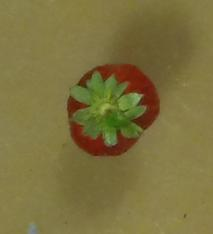
\includegraphics[width=\textwidth]{strawberry4_obj_01/strawberry4_001_32}
      \caption{}
  \end{subfigure}
  \begin{subfigure}[]{0.12\textwidth}
      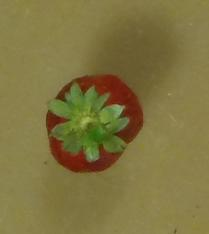
\includegraphics[width=\textwidth]{strawberry4_obj_01/strawberry4_001_30}
      \caption{}
  \end{subfigure}
  \begin{subfigure}[]{0.12\textwidth}
      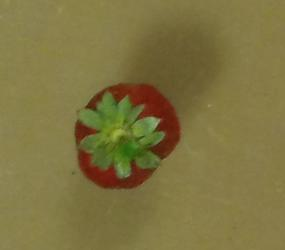
\includegraphics[width=\textwidth]{strawberry4_obj_01/strawberry4_001_28}
      \caption{}
  \end{subfigure}
  \begin{subfigure}[]{0.12\textwidth}
      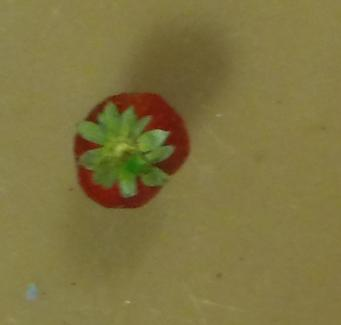
\includegraphics[width=\textwidth]{strawberry4_obj_01/strawberry4_001_26}
      \caption{}
  \end{subfigure}
  \begin{subfigure}[]{0.12\textwidth}
      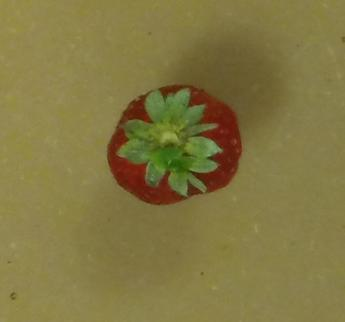
\includegraphics[width=\textwidth]{strawberry4_obj_01/strawberry4_001_24}
      \caption{}
  \end{subfigure}
  \begin{subfigure}[]{0.12\textwidth}
      \includegraphics[width=\textwidth]{strawberry4_obj_01/strawberry4_001_22}
      \caption{}
  \end{subfigure}
  \begin{subfigure}[]{0.12\textwidth}
      \includegraphics[width=\textwidth]{strawberry4_obj_01/strawberry4_001_20}
      \caption{}
  \end{subfigure}
  \begin{subfigure}[]{0.12\textwidth}
      \includegraphics[width=\textwidth]{strawberry4_obj_01/strawberry4_001_18}
      \caption{}
  \end{subfigure}
  \begin{subfigure}[]{0.12\textwidth}
      \includegraphics[width=\textwidth]{strawberry4_obj_01/strawberry4_001_16}
      \caption{}
  \end{subfigure}
  \begin{subfigure}[]{0.12\textwidth}
      \includegraphics[width=\textwidth]{strawberry4_obj_01/strawberry4_001_14}
      \caption{}
  \end{subfigure}
  \begin{subfigure}[]{0.12\textwidth}
      \includegraphics[width=\textwidth]{strawberry4_obj_01/strawberry4_001_12}
      \caption{}
  \end{subfigure}
  \begin{subfigure}[]{0.12\textwidth}
      \includegraphics[width=\textwidth]{strawberry4_obj_01/strawberry4_001_10}
      \caption{}
  \end{subfigure}
\caption[Images of a strawberry specimen after cropping a portion of background]{The strawberry specimen in Figure~\ref{fig:strawberry_height_specimen} shown after cropping a portion of the background}
\label{fig:strawberry_height_specimen_cropped}
\end{figure*}	

\begin{figure*}
  \centering
  \begin{subfigure}[]{0.12\textwidth}
      \includegraphics[width=\textwidth]{orange4_obj_11/orange4_011_32}
      \caption{}
  \end{subfigure}
  \begin{subfigure}[]{0.12\textwidth}
      \includegraphics[width=\textwidth]{orange4_obj_11/orange4_011_30}
      \caption{}
  \end{subfigure}
  \begin{subfigure}[]{0.12\textwidth}
      \includegraphics[width=\textwidth]{orange4_obj_11/orange4_011_28}
      \caption{}
  \end{subfigure}
  \begin{subfigure}[]{0.12\textwidth}
      \includegraphics[width=\textwidth]{orange4_obj_11/orange4_011_26}
      \caption{}
  \end{subfigure}
  \begin{subfigure}[]{0.12\textwidth}
      \includegraphics[width=\textwidth]{orange4_obj_11/orange4_011_24}
      \caption{}
  \end{subfigure}
  \begin{subfigure}[]{0.12\textwidth}
      \includegraphics[width=\textwidth]{orange4_obj_11/orange4_011_22}
      \caption{}
  \end{subfigure}
  \begin{subfigure}[]{0.12\textwidth}
      \includegraphics[width=\textwidth]{orange4_obj_11/orange4_011_20}
      \caption{}
  \end{subfigure}
  \begin{subfigure}[]{0.12\textwidth}
      \includegraphics[width=\textwidth]{orange4_obj_11/orange4_011_18}
      \caption{}
  \end{subfigure}
  \begin{subfigure}[]{0.12\textwidth}
      \includegraphics[width=\textwidth]{orange4_obj_11/orange4_011_16}
      \caption{}
  \end{subfigure}
  \begin{subfigure}[]{0.12\textwidth}
      \includegraphics[width=\textwidth]{orange4_obj_11/orange4_011_14}
      \caption{}
  \end{subfigure}
  \begin{subfigure}[]{0.12\textwidth}
      \includegraphics[width=\textwidth]{orange4_obj_11/orange4_011_12}
      \caption{}
  \end{subfigure}
  \begin{subfigure}[]{0.12\textwidth}
      \includegraphics[width=\textwidth]{orange4_obj_11/orange4_011_10}
      \caption{}
  \end{subfigure}
\caption[Images of an orange specimen after cropping a portion of background]{The orange specimen in Figure~\ref{fig:orange_height_specimen} shown after cropping a portion of the background}
\label{fig:orange_height_specimen_cropped}
\end{figure*}	


\subsection{Annotation Process}
\label{sec:distdes_annotation}

The task of manual image annotation is a costly and labor-intensive process. Developing an object recognition algorithm is often motivated by a desire to avoid manual inspection in order to identify objects from images. However, in order to build a machine learning framework for object recognition, an initial set of images needs to be annotated manually and become the learning set. 
Just like any other supervised machine learning algorithm, this procedure requires annotation of images into labeled foreground and background. Here, each learning sample consists of $t$ images of a specimen captured from different heights. Increasing the number of images of each specimen quickly increases the annotation load. To mitigate this burden, a semi-automated annotation framework is developed.

In the first stage of the annotation process, a customized \gls{buva} technique (described in Section~\ref{sec:visual_attn}) is used to pick the most \textit{interesting} point in an image. This most \textit{interesting} point is referred to as the first fixation. According to the visual attention hypothesis, if a distribution of features can be used to characterize an image, the first fixation corresponds to the point in the image which is most unlikely to belong to this distribution of features. In other words, the first fixation supposedly corresponds to a point that does not belong to the background (and hence most likely it is a foreground object pixel). In the first stage of this semi-automated annotation process, the first fixation point along with all its neighboring pixels are assumed to be foreground pixels. Thus a rectangle of dimensions $15\%$ image width $\times 15\%$ image height, centered on the fixation is assumed to be part of the foreground region. This rectangle is referred to henceforth as the \textit{foreground 
hypothesis rectangle}.
Since the data collection  process ensures that an object in an image is close to the center of the image rather than the boundary, the pixels in the boundary of the images can safely be assumed to be background pixels. Hence, rectangular blocks of pixels in the 4 corners of an image are assumed to be background pixels. Each of these background blocks is $5\%$ image width $\times 5\%$ image height in dimension. This foreground and background pixel hypothesis is used in the next stage of the annotation process to segment the image into foreground and background. A visual representation of the background and foreground seed pixels is shown in Figure~\ref{fig:good_seg_visualattn_seeds} as blue and red rectangles, respectively. The visual attention fixation is shown here as a green dot.

The foreground and background seeds thus obtained can be used to initialize a grabcut-in-one-cut algorithm \cite{onecut}. This grabcut-in-one-cut algorithm, a variant of graphcut algorithm (described in Section~\ref{sec:onecut}) splits an input image into background and foreground. Grabcut-in-one-cut algorithm operates by labeling pixels \textit{similar} in appearance to foreground seeds as foreground and the other pixels that appear closer to background seeds as background.
However, the foreground seeds supplied by visual attention, might not produce accurate results in \emph{all} cases. There are occasionally instances when the fixation tagged as foreground includes pixels from the object's boundary. Since object boundary pixels are essentially discontinuities, indicating a transition between foreground and background pixel distributions, the likelihood of visual attention picking them as fixations is relatively high. If an object's boundary pixel is picked as the first fixation, this could result in the foreground hypothesis rectangle erroneously containing background pixels. An illustration of this effect is given in Figure~\ref{fig:good_seg_visualattn_seeds} where the green dot at the boundary of the object is the visual attention fixation. The blue foreground hypothesis rectangle around the fixation point contains some wrongly labeled background pixels. Wrongly labeled background pixels in foreground seeds supplied to graphcut algorithm can result in inaccurate segmentation, as in the case seen in 
Figure~\ref{fig:good_seg_visualattn_seg}. Thus, to improve the performance of the graphcut algorithm, that iteratively refines the foreground seeds is used. Iterative refinement works by taking the result of the graphcut segmentation, computing the centroid of the foreground pixels, and utilizing a foreground hypothesis rectangle around this centroid as input foreground seed to the next iteration of this iterative graphcut algorithm. This process is repeated until the segmentation results stabilize. Specifically, this iterative graphcut process is repeated 
until the number of foreground pixels from the previous iteration, rejected as background by the current iteration, is within a small threshold of 5\%. If $F_i$ is the set of foreground pixels labeled by the graphcut algorithm in iteration $i$, then the iterative process is continued till the condition below is satisfied.
%
\begin{equation}
 \label{eqn:seg_threshold}
 \frac{|F_{i-1}-F_{i}|}{|F_i|} \leq 0.05\enspace .
\end{equation}
%
%
\begin{figure*}
  \centering
  \begin{subfigure}[]{0.2\textwidth}
      \includegraphics[width=\textwidth]{distdes_annotation_good_visualattn_seeds}
      \caption{}
      \label{fig:good_seg_visualattn_seeds}
  \end{subfigure}
  \begin{subfigure}[]{0.2\textwidth}
      \includegraphics[width=\textwidth]{distdes_annotation_good_visualattn_segment}
      \caption{}
      \label{fig:good_seg_visualattn_seg}
  \end{subfigure}
  \begin{subfigure}[]{0.2\textwidth}
      \includegraphics[width=\textwidth]{distdes_annotation_good_recursive_seeds}
      \caption{}
      \label{fig:good_seg_recursive_seeds}
  \end{subfigure}
  \begin{subfigure}[]{0.2\textwidth}
      \includegraphics[width=\textwidth]{distdes_annotation_good_recursive_segment}
      \caption{}
      \label{fig:good_seg_recursive_seg}
  \end{subfigure}
\caption[Illustration of annotation process flow]{An illustration of operation of visual attention and recursive graphcut as a part of the annotation process flow is shown here. (\subref{fig:good_seg_visualattn_seeds}) shows the visual attention fixation as a green dot. Since the visual attention fixation is on the boundary of the object, the foreground hypothesis rectangle shown in blue contains background pixels. When the graphcut algorithm operates on (\subref{fig:good_seg_visualattn_seeds}) utilizing the pixels inside the blue rectangle as the foreground seeds and the pixels inside the red rectangles as the background seeds, the resulting segmented foreground region is displayed in (\subref{fig:good_seg_visualattn_seg}). Due to the presence of background pixels in the input foreground seeds, the segmentation result obtained in (\subref{fig:good_seg_visualattn_seg}) is inaccurate. When recursive graphcut algorithm is 
applied, the blue foreground hypothesis rectangle eventually moves towards the center of the object (as seen in (\subref{fig:good_seg_recursive_seeds})) and no longer contains background pixels. With the updated foreground hypothesis rectangle after recursive graphcut segmentation, the improved segmentation result can be seen in (\subref{fig:good_seg_recursive_seg}).}
\label{fig:annotation_good_seg}
\end{figure*}	
%
The change in the blue foreground hypothesis rectangle after recursive graphcut segmentation and the resulting improved foreground labeling can be seen in Figure~\ref{fig:good_seg_recursive_seeds} and Figure~\ref{fig:good_seg_recursive_seg} respectively.
When the foreground region labels from the graphcut algorithm stabilize, it is unlikely that the foreground region will change after subsequent iterations. This stabilization condition captured in \eqref{eqn:seg_threshold}, indicates that the foreground region label hypothesis generated by graphcut has converged. In case the convergence condition in \eqref{eqn:seg_threshold} is not met after $N$ iterations ($N$ here is taken equal to $5$), further recursion is abandoned and the labeling results available after $N$ iterations are adopted by default.

Though this process appears to be fully automated, there are cases where this automated segmentation fails. A case of segmentation failure could be due to visual attention picking up \emph{interesting} artifacts in the image that are not necessarily part of the specimen. There are also cases where the texture of the specimen is not uniform, in which case visual attention could be biased towards a specific part of the object. This could result in graphcut segmentation only identifying the sub-region of the specimen that biased the visual attention fixation. An instance of only segmenting a sub-region of the specimen is often seen in cases of strawberries, which are characterized by the occurrence of a green stalk on top of a reddish pulp. Visual attention and graphcut could end up mistakenly segmenting either the green stalk or the red pulp only. This case is illustrated in Figure~\ref{fig:annotation_bad_seg}. The visual attention fixation shown by a green dot in Figure~\ref{fig:bad_seg_visualattn_seeds} is 
biased towards the green stalk region of the strawberry specimen. An application of recursive graphcut on this example only ends up segmenting the green stalk region as seen in Figure~\ref{fig:bad_seg_recursive_seg}. This error in segmentation can be rectified through inclusion of appropriate foreground seeds that are representative of the complete specimen, i.e., both the green stalk and the red pulp sub-regions in case of strawberry. Therefore, to prevent inaccurate segmentation from degrading the learning set, a manual verification process is added as the last step of this annotation process. During this process, for all failed instances of automated segmentation, the foreground and background seed pixels are manually set. 
%
\begin{figure*}
  \centering
  \begin{subfigure}[]{0.2\textwidth}
      \includegraphics[width=\textwidth]{distdes_annotation_bad_visualattn_seeds}
      \caption{}
      \label{fig:bad_seg_visualattn_seeds}
  \end{subfigure}
  \begin{subfigure}[]{0.2\textwidth}
      \includegraphics[width=\textwidth]{distdes_annotation_bad_recursive_segment}
      \caption{}
      \label{fig:bad_seg_recursive_seg}
  \end{subfigure}
\caption[Illustration of a case where automated annotation process fails]{An illustration of a case where automated annotation process fails, and human verification and correction is required. The visual attention fixation shown as a green dot in (\subref{fig:good_seg_visualattn_seeds}) is biased towards the green stalk region of the strawberry. Since this strawberry specimen exhibits binary texture--green stalk and red pulp, the combined visual attention and graphcut automated annotation approach ends up segmenting only the stalk sub-region of this strawberry specimen (see (\subref{fig:bad_seg_recursive_seg})). Such cases of failure calls for human verification and correction of foreground seeds to enable graphcut algorithm to segment the whole strawberry specimen.} 
\label{fig:annotation_bad_seg}
\end{figure*}	
%

This final manual verification and correction process requires human effort. However, during experiments it was noted that a very small percentage of cases needed corrective action. In summary, this semi-automated annotation process is relatively effective and significantly less cumbersome than a fully manual annotation effort. An illustration of the output of this annotation process for a single specimen of orange is given in Figure~\ref{fig:orange_segment_height_montage}. Figure~\ref{fig:orange_segment_height_montage} represents a montage of $t=12$ images of an orange specimen with the top-left component showing the segmented foreground from the image captured $d_{max}=32$ inches away from the orange specimen. Likewise, the bottom-right shows the image that was captured $d_{min}=10$ inches away from the specimen. The montage in Figure~\ref{fig:orange_segment_height_montage} is arranged such that the 12 images, from left to right, are in decreasing order of height.
%
\begin{figure*}
  \centering
  \includegraphics[width=\textwidth]{orange_height_segment_montage_12}
  \caption[Annotation output for a single specimen]{The output of the annotation process showing a montage of the segmented foreground from a set of $t=12$ images that belong to a single orange specimen. The left-top montage component is the image of the orange specimen captured $d_{max}=32$ inches from the ground. The montage components arranged from left to right (with wrap-around after every 4 images) to progressively show images that were captured closer to the orange specimen. The closest image that was captured is $d_{min}=10$ inches away from the specimen and is shown in the bottom-most row.} 
  \label{fig:orange_segment_height_montage}
\end{figure*}	
%


\subsection{Learning}


The learning phase of a machine learning based object recognition method involves identifying patterns in the data that represent the presence of an object. The information fed to a machine learning algorithm is a pre-specified labeling of the data into foreground and background. The responsibility of the learning method here is to identify patterns in designated foreground regions, using information from labeled background to reject false positives. The patterns identified by the learning algorithm are then channeled into the construction of a classifier that is capable of identifying foreground pixels from an image.

In the machine learning technique proposed in this chapter, instead of using individual images with annotations of foreground and background, a collection of $t$ images each featuring the same specimen from a known height is utilized. The goal is to encode the variation in appearance of a specimen from different heights to build a robust object recognition classifier. Height offers an additional dimension in the feature space for the learning algorithm to capitalize on.

This object recognition algorithm is designed to operate on images without prior segmentation. That is, the features used in this algorithm should be sufficiently generic to capture the appearance of an object directly from an image without foreground segmentation. To achieve this, we use the histogram signatures (described in Section~\ref{sec:hist_signature}) to extract information from an image in \gls{hsi} colorspace. The histogram information from multiple specimens of the same object class is then combined to generate a feature distribution. The details of this process are described below.

\subsubsection{The Feature Distribution}
\label{sec:distdes_feature_distr}

The first step in computing this feature distribution is the computation of the hue, saturation and intensity histogram signatures on the labeled foreground pixels in the learning dataset. The parameters chosen for the histogram signature computation are the number of equally spaced histogram bins, here, $|\mathcal{B}|=256$, and the upper bound on the number of pixels affected by noise, here, $e=5\%$. Using these parameters the histogram signatures for all three components of the \gls{hsi} colorspace are calculated for all $t=12$ height-tagged images of a specimen. Note that this histogram signature computation only utilizes the labeled foreground pixels in the image. Let the histogram signature of the labeled foreground for specimen $k$, with height tag $h$, belonging to class $c$, on the color component $f\in\{H \text{ hue}, S \text{ saturation}, I \text{ intensity}\}$ be represented as $\mathcal{H}^{c_{hk}}_f$. Since there are 3 color components, we generate 3 histogram signatures per height-tagged specimen image. If we 
consider all the $t$ height-tagged images available for a specimen, the total histogram signatures now available is $3\times t$, that is, 36 for this experimental study.

In the next stage of the learning process, the histogram signatures $\mathcal{H}^{c_{hk}}_f$ from all specimens belonging to a single object class are combined to generate a generalized histogram signature for the object class.
In order to achieve this, the mean of all histogram signatures corresponding to a specific height-tag from all specimens of a class are combined. In other words, the mean $\bar{\mathcal{H}}^{c_{h}}_f$ of all histogram signatures with height-tag $h$ is computed by taking the mean of individual components of the $256$-dimensional vectors of sequence-of-histogram signatures $\mathcal{H}^{c_{h1}}_f, \mathcal{H}^{c_{h2}}_f, \mathcal{H}^{c_{h3}}_f, \ldots, \mathcal{H}^{c_{hm}}_f$, where $m$ is the number of specimens of class $c$ available in the learning dataset. Technically, the $j$-th component of the $256$-dimensional mean histogram $\bar{\mathcal{H}}^{c_{h}}_f$ is found as
\begin{align}
 \left[\bar{\mathcal{H}}^{c_{h}}_f\right]_j=\frac{1}{m}\sum_{k=1}^{m} \left[ \mathcal{H}^{c_{hk}}_f \right]_j.
\end{align}
Since there are $t$ different height-tags along with 3 different color components, each object class $c$ is represented by a sequence of $3t$ histogram signatures, which will be collectively referred to as $\bar{\mathcal{H}}^{c}$.

The sequence of $3t$ histogram signatures $\bar{\mathcal{H}}^{c}$ captures the generalized appearance of the objects of class $c$. Its important to note that the data used to compute this generalized histogram signature are composed of foreground pixels of object specimens only, without any background information. If we are to use such a generalized histogram signature generated only from foreground information for classifying objects, it is necessary to pre-process an image to detect and segment objects present in the images before this generalized histogram signature $\bar{\mathcal{H}}^{c}$ can be used for classification purposes. However, one of the goals of this work is to avoid segmentation while attempting classification of objects from images. To realize this goal, we revisit the learning dataset, and use the background information to build a representation that captures how inclusion of background pixels to different individual histogram signatures affects the generalized histogram signature $\bar{
\mathcal{H}}^{c}$ of class $c$. 

In order to use background information for building such a classifier, we first generate another set of histogram signatures.
For specimen $k$ of class $c$ from the learning dataset, we compute a sequence of $3t$ histogram signatures similar to the computation involved in $\mathcal{H}^{c_{hk}}_f$, but now utilizing all pixels in the image instead of just the foreground pixels. This set of $3t$ histograms $\ddot{\mathcal{H}}^{c_{k}}$ for specimen $k$ of class $c$ is given by
\begin{align}	\label{eqn:hist_signature}
 \ddot{\mathcal{H}}^{c_{k}} = \ddot{\mathcal{H}}^{c_{hk}}_f \Big|_{h\times f}\enspace ,
\end{align}
%
here $h\in\{10,12, \ldots,32\}$ and $f\in\{H,S,I\}$.

Once we have the sequence of histogram signatures $\ddot{\mathcal{H}}^{c_{k}}$ of specimen $k$ belonging to class $c$, along with the generalized histogram signature $\bar{\mathcal{H}}^{c}$ of class $c$, a numeric distance measure $D$ between the histogram signatures can be computed. If we have a series of such distance measures evaluated for a collection of specimens of class $c$, a distribution of these distance measures can be generated. This distribution 
of distance measures encodes the variability in generalized histogram signature $\bar{\mathcal{H}}^{c}$ induced by the presence of background pixels along with foreground pixels. In effect, this offers a way to check images for the presence of an object of class $c$ without any prior segmentation of foreground pixels. The distance measure is the standard \emph{$L_2$-norm} between two vectors.
%
\begin{align}	\label{eqn:hist_signature_dist}
 d_{chfk} = D(\bar{\mathcal{H}}^{c_{h}}_f, \ddot{\mathcal{H}}^{c_{hk}}_f) 
 = \sqrt{\sum_{j=1}^{|B|}\Bigg(\left[\bar{\mathcal{H}}^{c_{h}}_f\right]_j
 -\left[\ddot{\mathcal{H}}^{c_{hk}}_f\right]_j\Bigg)^2}
\end{align}

Since there are $3t$ histograms in total, we get a sequence of $d_{chfk}$ values of length $3t$ for the $k$-th specimen of class $c$, and this sequence is represented as
%
\begin{align}	\label{eqn:dist_sequence}
 D_{ck}=d_{chfk}\Big|_{h\times f}\enspace .
\end{align}
%

A sequence of distance measures $D_{ck}$ for each specimen $k$ among the $m$ specimens of class $c$ provides a representation of a feature vector of size $3t$ that describes the appearance of an image that contains a specimen of class $c$. If we consider the feature vectors of all the $m$ available specimens $D_{c1},D_{c2},\ldots,D_{cm}$, a feature distribution sequence $F_c$ that represents the appearance of images containing objects of class $c$ can be formulated. Lets assume that the $m$ values $d_{chf1}, d_{chf2},\ldots,d_{chfm}$ are drawn from a normal distribution 
%
\begin{align}
 F_{chf}\sim &\mathcal{N}(\mu_{chf},\sigma^2_{chf})\label{eqn:normal_distr}\\
 \mu_{chf}= &\frac{\sum_{k=1}^m d_{chfk}}{m}\label{eqn:normal_mean}\\
 \sigma^2_{chf}= &\frac{\sum_{k=1}^m (d_{chfk}-\mu_{chf})^2}{m-1}\label{eqn:normal_stddev}\enspace .
\end{align}
%
Then the feature distribution sequence
\begin{align}	\label{eqn:feat_distribution}
 F_c=F_{chf}\Big|_{h \times f}
\end{align}
can be represented as a sequence of $3t$ distributions. 

For the two classes of objects, strawberries and oranges with 11 specimens each, the respective feature distributions $F_s$ and $F_o$ can thus be computed. The feature distributions $F_s$ and $F_o$ are shown in Figure~\ref{fig:feat_distr}. The $3t=36$ distributions (see \eqref{eqn:feat_distribution}) in the distribution sequence are shown along the $x$-axis. Each distribution here is represented by a dot and a bar adjoining it. The dot corresponds to the mean and the bar corresponds to the 95\% confidence interval, or the $2\sigma$ standard deviation interval of the distribution shown in \eqref{eqn:normal_distr}.
%
\begin{figure*}
  \centering
  \begin{subfigure}[]{0.8\textwidth}
      \includegraphics[width=\textwidth]{strawberry_learning_feature_distribution_12}
      \caption{}
      \label{fig:feat_distr_strawberry}
  \end{subfigure}
  \begin{subfigure}[]{0.8\textwidth}
      \includegraphics[width=\textwidth]{orange_learning_feature_distribution_12}
      \caption{}
      \label{fig:feat_distr_orange}
  \end{subfigure}
\caption[Feature distribution]{Strawberry feature distribution sequence $F_s$ (\subref{fig:feat_distr_strawberry}) and orange feature distribution sequence $F_o$ (\subref{fig:feat_distr_orange}) generated from 11 strawberry specimens and 11 orange specimens. All $3t=36$ distributions indexed by $v$ are shown along the $x$-axis. The  mean of each distribution is shown as a dot along with the 95\% confidence interval shown as a bar.}
\label{fig:feat_distr}
\end{figure*}	
%

This feature distribution $F_c$, which comprises a sequence of $3t$ distributions, offers a way to test for the presence of an object of class $c$ in an image without prior segmentation. In essence, the testing for the presence of an object can be broken down into $3t$ individual hypothesis tests. Each hypothesis test checks whether a certain colorspace-specific height-tagged image containing an object satisfies a specific distribution, among the $3t$ distributions in $F_c$. Not all of the $3t$ hypothesis tests might be equally informative-- some of them could be more relevant than others. To this end, a weighting factor $w_{v}$ can be attached to the $v$-th element in feature distribution sequence $F_c$.  More details regarding the computation of these weight factors is described below.

\subsubsection{Feature Weights}
\label{sec:distdes_feat_wts}

The feature weights offer a way to weight each distribution in the feature distribution sequence $F_c$. In case of a binary classification problem between objects of class $p$ and $q$, we choose the feature weights such that the distributions in the sequence with lower intra-class variance are weighted higher compared to other distributions. Additionally, the magnitude of the overlap between identical indexed distributions in $F_p$ and $F_q$ also influences the weights. In the rest of this section the formulation of these feature weights is discussed.

For object class $p$ and object class $q$, the corresponding feature distribution sequences $F_p$ and $F_q$ are in both cases sequences of $3t$ normal distributions. Let the $v$-th component of sequence $F_p$ be denoted $F_{pv}\sim\mathcal{N}(\mu_{pv},\sigma^2_{pv})$.
The the 95\% confidence interval of $F_{pv}$ is given by
%
\begin{align}	\label{eqn:conf_interval}
C^{0.95}_{F_{pv}}=[\mu_{pv}-2 \times \sigma_{pv},\, \mu_{pv}+2 \times \sigma_{pv}]\enspace .
\end{align}
%
The weight $w_{pv}$ of the $v$ component of $F_p$ is given by
\begin{align}
 w'_{pv}= & \frac{1}{(1+ |C_{F_{pv}} \cap C_{F_{qv}}| )\times \sigma_{pv}} \label{eq:feat_wt}\\
 w_{pv}= & \frac{w'_{pv}}{\sum_{j} w'_{pj}} \label{eqn:feat_wt_norm}
\end{align}
where $|C_{F_{pv}} \cap C_{F_{qv}}|$ corresponds to the length of the interval obtained after the intersection of intervals $C_{F_{pv}}$ and $C_{F_{qv}}$. The first term in the denominator of \eqref{eq:feat_wt}, $1+ |C_{F_{pv}} \cap C_{F_{qv}}|$, penalizes distributions whose confidence intervals share common positions with an identical indexed distribution in the other class. In other words, this term penalizes distribution $F_{pv}$ whose confidence interval overlaps with intervals of an identical indexed distribution $F_{qv}$. The second term in the denominator of \eqref{eq:feat_wt}, $\sigma_{pv}$, penalizes distributions with high intra-class variance. Ultimately, the weights are normalized as shown in \eqref{eqn:feat_wt_norm}. The $3t$ feature weights thus computed for a class will collectively be referred to as $W_c$. For the binary classification problem, between strawberry and orange specimens, the weight factors computed using \eqref{eqn:feat_wt_norm} are shown in the bar plot in Figure~\ref{fig:feat_weights}. The black bars show the strawberry 
class 
weights and the red 
bars show the corresponding orange-class weights.
%
\begin{figure}
  \centering
  \includegraphics[width=\textwidth]{feature_weights_12}
  \caption[Feature weights]{The feature weights for strawberry-class $F_s$ (black bars) and orange-class $F_o$ (red bars)}
  \label{fig:feat_weights}
\end{figure}	
%

The distribution components in $F_p$ with higher values of $w_p$ are weighted higher than the other distributions while performing hypothesis tests. This is discussed in the next section on validation phase of this machine learning algorithm.

\subsection{Validation}
\label{sec:distdes_validation}


In this object recognition method, a series of height-tagged images of an object specimen is used to perform a binary classification task. In other words, the $t$ height-tagged images are used to decide if the object belongs to one of the two classes: $p$ or $q$. In order to achieve this, the histogram signatures (described in Section~\ref{sec:hist_signature}) are computed on each of the $t$ height tagged-images available for an object specimen. Since there is no pre-specified label information available, all pixels in the image are used here. The computation performed is identical to the one in \eqref{eqn:hist_signature}, and results in a sequence of $3t$ histogram signatures $\ddot{\mathcal{H}}^{k}$. 

The next step in the validation procedure is to use \eqref{eqn:hist_signature_dist} and \eqref{eqn:dist_sequence} to compute the distance measure sequences $D^p_k=D(\ddot{\mathcal{H}}^{k}, \bar{\mathcal{H}}^{p})$ and $D^q_k=D(\ddot{\mathcal{H}}^{k}, \bar{\mathcal{H}}^{p})$. The $3t$-value sequences $D^p_k$ and $D^q_k$ provide information on how \emph{close} to each of the classes $p$ and $q$, the sample specimen $k$ is. The information in these sequences need to be processed further in order to associate specimen $k$ with either class $p$ or class $q$.

Let us assume that specimen $k$ belongs to class $p$. According to this hypothesis, the $v$-th component of $D^p_k$ should follow the $v$-th distribution of the feature distribution sequence $F_p$. In other words, using \eqref{eqn:conf_interval}, we can state with 95\% \textit{confidence} that condition 
%
\begin{align}
  d^p_{kv} \in C^{0.95}_{F_{pv}}= &[\mu_{pv}-2 \times \sigma_{pv},\, \mu_{pv}+2 \times \sigma_{pv}]
  \label{eqn:conf_interval_validation}
\end{align}
%
is satisfied. If we call this hypothesis test $h^p_{kv}$, then passing of this hypothesis test
%
\begin{align}
 h^p_{kv} = &
 \begin{cases}
    1	&	d^p_{kv} \in C^{0.95}_{F_{pv}}\\
    0	&	otherwise
 \end{cases} \label{eqn:hypothesis_test}
\end{align}
%
meaning $(h^p_{kv}=1)$, determines that specimen $k$ belongs to class $p$.

There are $3t$ such hypothesis tests, $h^p_{k1}, h^p_{k2},\ldots, h^p_{k\, 3t}$ that can be performed to determine if specimen $k$ belongs to class $p$.
The importance of each of these hypothesis tests for associating specimen $k$ with class $p$ is determined by the corresponding weight $w_{pv}$. The information available in the form of hypothesis tests, along with their associated weights, is combined in to a single numeric metric or \emph{class confidence} 
%
\begin{align} \label{eqn:numeric_class_metric}
 H^p_k=\sum_{v=1}^{3t} h^p_{kv} w_{pv} 
\end{align}
%
that measures the confidence in specimen $k$ belonging to class $p$.

It is important to note that based on ~\eqref{eqn:feat_wt_norm}, it follows that $H^p_c\in[0,1]$. If $H^p_k=1$, then we can say with high confidence that specimen $k$ belongs to class $p$. Alternatively, $H^p_k=0$ suggests that its unlikely that specimen $k$ belongs to class $p$. A similar metric $H^q_k$ is computed to determine confidence in the assertion that
specimen $k$ belongs to class $q$. Finally, the binary classification task that classifies specimen $k$ into class $p$ or class $q$ is decided based on the magnitude of $H^p_k$ and $H^q_k$:
%
\begin{align}	\label{eqn:binary_classification}
 H^p_k > H^q_k	&{} &\text{specimen}\, k \in \text{class}\, p\nonumber\\
 H^p_k < H^q_k	&{} &\text{specimen}\, k \in \text{class}\, q\nonumber\\
 H^p_k = H^q_k	&{} &\text{Undetermined}
\end{align}


%================================================================================================================
\section{Results}

The data collected during the experiments involve images from 11 specimens of both orange-class and strawberry-class. Data on each specimen included images taken from $t=12$ different heights, starting at $d_{max}=32$ inches from the ground, down to $d_{min}=10$ inches, away from the ground. The imaging experiment was conducted in a test tank filled with water using the imaging rig shown in Figure~\ref{fig:im_rig}. More details of the data collection process can be found in Section~\ref{sec:distdes_data_collection}. Following the data collection process, the feature distribution sequence $F_{s}$ for strawberry-class, and $F_{o}$  for orange-class, are computed using the procedure discussed in Section~\ref{sec:distdes_feature_distr}; the results are shown in Figure~\ref{fig:feat_distr}.

As part of an initial validation step, both learning and testing is done on the entire dataset of 22 specimens (11 strawberries and 11 oranges). The learning procedure
results in feature distributions for strawberry and orange which are are shown in Figure~\ref{fig:feat_distr}. Then each specimen is evaluated against both strawberry and orange feature distributions as described in Section~\ref{sec:distdes_validation}, to get distance metric sequences $D^s_k$ and $D^o_k$. The 11 strawberry specimens are checked against the strawberry and orange feature distribution sequences $F_{s}$ and $F_{o}$; see Figure~\ref{fig:feat_results_strawberry_test}. The black bars in Figure~\ref{fig:feat_results_strawberry_test_strawberry_learn} are the 95\% confidence intervals of strawberry feature distribution sequence $F_{s}$ (this is identical to Figure~\ref{fig:feat_distr_strawberry}).
The colored points in Figure~\ref{fig:feat_results_strawberry_test_strawberry_learn} represent the distance metric sequences $D^s_k$ of the 11 strawberry specimens (points with the same color across the x-axis come from a single strawberry specimen). Along side each black bar (in the y-dimension), we see 11 data points (each one comes from a different strawberry specimen).
Most of these colored points lie inside the confidence intervals indicating that the 
distance metric sequence $D^s_k$ of strawberry specimens are in agreement with the strawberry-class distribution sequence $F_{s}$.
In Figure~\ref{fig:feat_results_strawberry_test_orange_learn}, we compare the same 11 strawberry specimens against the orange-class distribution sequence $F_{o}$. In this case, the black bars representing the 95\% confidence interval of orange-class distribution sequence $F_{o}$ is identical to 
Figure~\ref{fig:feat_distr_orange}. The colored points here represent the distance metric sequence $D^o_k$ values for the 11 strawberry specimens.
In contrast to Figure~\ref{fig:feat_results_strawberry_test_strawberry_learn}, the colored points in Figure~\ref{fig:feat_results_strawberry_test_orange_learn} are often not in agreement with the confidence intervals of the orange-class feature distribution sequence $F_{o}$.
This is a clear indicator of strawberry specimens matching better with the strawberry-class feature distribution $F_s$ compared to orange-class feature distribution $F_o$. On similar lines, the 11 orange specimens are compared against the orange-class feature distribution $F_{o}$ in Figure~\ref{fig:feat_results_orange_test_orange_learn} and also compared against strawberry-class feature distribution $F_{s}$ in Figure~\ref{fig:feat_results_orange_test_strawberry_learn}. The observations show that the orange specimens match closer with orange feature distribution sequence $F_{o}$ rather than the strawberry feature distribution sequence $F_{s}$. This again reinforces that the distance metric 
values of both orange and strawberry specimens agree with their corresponding class distribution sequences.

%
\begin{figure*}
  %\vskip -12pt
  \centering
  \begin{subfigure}[]{0.6\textwidth}
      \includegraphics[width=\textwidth]{validation_strawberry_testset_strawberry_learnset_12}
      \caption{Strawberry specimens evaluated against strawberry feature distribution sequence $F_s$}
      \label{fig:feat_results_strawberry_test_strawberry_learn}
  \end{subfigure}
  \begin{subfigure}[]{0.6\textwidth}
      \includegraphics[width=\textwidth]{validation_strawberry_testset_orange_learnset_12}
      \caption{Strawberry specimens evaluated against orange feature distribution sequence $F_o$}
      \label{fig:feat_results_strawberry_test_orange_learn}
  \end{subfigure}
\caption[Strawberry specimen validation results]{Validation results obtained 
while evaluating strawberry specimens against 
strawberry-class feature distribution sequence $F_s$ (\subref{fig:feat_results_strawberry_test_strawberry_learn}) and against the
orange-class feature distribution sequence $F_o$ 
(\subref{fig:feat_results_strawberry_test_orange_learn}). The strawberry-class feature distribution sequence $F_s$ is shown in (\subref{fig:feat_results_strawberry_test_strawberry_learn}): the 95\% confidence intervals are shown as black bars with the mean of a distribution shown as a black dot in the center of the corresponding black bar. The sequence of feature distributions indexed by $v$ are identical to Figure~\ref{fig:feat_distr_strawberry}. The colored dots in (\subref{fig:feat_results_strawberry_test_strawberry_learn}), represent the distance metric sequence $D^s_k$ of the 11 strawberry specimens (dots of the same color come from a single specimen). Along y-axis, we see a series of 11 points next to each black bar. Each of these 11 points come from a single strawberry specimen. The vast majority of the colored dots in (\subref{fig:feat_results_strawberry_test_strawberry_learn}) lie inside the corresponding confidence intervals, indicating that the distance metric values of strawberry specimens are in agreement with the 
strawberry-class distribution sequence $F_s$.
In (\subref{fig:feat_results_strawberry_test_orange_learn}), the same 11 strawberry specimens are checked against the orange-class feature distribution sequence $F_o$. In this case, the black bars are representative of the orange-class feature distribution sequence $F_o$. In contrast to (\subref{fig:feat_results_strawberry_test_strawberry_learn}), a sizable percentage of colored dots in (\subref{fig:feat_results_strawberry_test_orange_learn}) do not agree with the orange-class feature distribution sequence $F_o$. This signifies that the strawberry specimens primarily agree with the strawberry feature distribution sequence $F_s$ and not with orange distribution sequence $F_o$.}
\label{fig:feat_results_strawberry_test}
\end{figure*}	
%
\begin{figure*}
  \vskip -12pt
  \centering
  \begin{subfigure}[]{0.6\textwidth}
      \includegraphics[width=\textwidth]{validation_orange_testset_orange_learnset_12}
      \caption{Orange specimens evaluated against orange feature distribution sequence $F_o$}
      \label{fig:feat_results_orange_test_orange_learn}
  \end{subfigure}
  \begin{subfigure}[]{0.6\textwidth}
      \includegraphics[width=\textwidth]{validation_orange_testset_strawberry_learnset_12}
      \caption{Orange specimens evaluated against strawberry feature distribution sequence $F_s$}
      \label{fig:feat_results_orange_test_strawberry_learn}
  \end{subfigure}
\caption[Orange specimen validation results]{Similar to Figure~\ref{fig:feat_results_strawberry_test} that shows the validation results for strawberry specimens, this figure shows the validation results for orange specimens. Testing of orange specimens against 
orange-class feature distribution sequence $F_o$ is shown in 
(\subref{fig:feat_results_orange_test_orange_learn}), and testing against the
strawberry-class feature distribution sequence $F_s$ is shown in
(\subref{fig:feat_results_orange_test_strawberry_learn}). 
The orange-class feature distribution sequence $F_o$ is shown in (\subref{fig:feat_results_strawberry_test_strawberry_learn}): the 95\% confidence intervals are shown as black bars with the mean of a distribution shown as a black dot in the center of the corresponding black bar. The sequence of feature distributions indexed by $v$ are identical to Figure~\ref{fig:feat_distr_orange}. The colored dots in (\subref{fig:feat_results_orange_test_orange_learn}), represent the distance metric sequence $D^o_k$ of the 11 orange specimens (dots of the same color come from a single specimen). Along y-axis, we see a series of 11 points next to each black bar. Each of these 11 points come from a single orange specimen. The vast majority of the colored dots in (\subref{fig:feat_results_orange_test_orange_learn}) lie inside the confidence intervals indicating that the distance metric values of orange specimens are in agreement with the orange-class distribution sequence $F_o$.
In (\subref{fig:feat_results_orange_test_strawberry_learn}), the same 11 orange specimens are considered against the strawberry-class feature distribution sequence $F_s$. In this case, the black bars are representative of the strawberry-class feature distribution sequence $F_s$. In contrast to (\subref{fig:feat_results_orange_test_orange_learn}), the colored dots in (\subref{fig:feat_results_orange_test_strawberry_learn}) do not agree with the confidence intervals of strawberry-class feature distribution sequence $F_s$. This signifies that the orange specimens primarily agree with the orange feature distribution sequence $F_o$ and not with strawberry distribution sequence $F_s$.}
\label{fig:feat_results_orange_test}
\end{figure*}	
%

A more concrete validation of this machine learning approach is by computing the \emph{class confidence} $H^s_k$ and $H^o_k$ of each specimen, and deciding on the class of the specimen as described in Section~\ref{sec:distdes_validation}. One thing to note here is that the class confidence measure requires the feature distribution sequences of the strawberry and orange classes to be computed. The feature distribution sequences are generated from the learning set, which contains the specimen we are currently trying to recognize. Wanting to separate the learning and testing datasets before validation, and because the number of specimens is small, a leave-one-out cross-validation \cite{alpaydin} was implemented.\footnote{Leave-one-out cross-validation is used in cases where the number of specimens available is very small. In such cases, one does not have the luxury of splitting the available labeled dataset into 
learning and testing sets. Therefore, in leave-one-out cross-validation, during each iteration one 
specimen is chosen as the testing set and the all other specimens are chosen as the learning set. Thus the learning procedure is repeated in each iteration, without adding the instance that is being tested to the learning set.} The class confidence values $H^s_k$ and $H^o_k$ of the 11 strawberry specimens are shown as black and red bars respectively in Figure~\ref{fig:results_strawberry}. It is clear that the black bars are taller than the red bars in all cases. According to the hypothesis test in force (see \eqref{eqn:hypothesis_test}), this implies that that all strawberry specimens are classified correctly. The same can be said for the orange specimens. As seen in Figure~\ref{fig:results_orange}: all the red bars are taller than the back bars. Therefore, all orange specimens are also classified correctly.

%
\begin{figure*}
  \centering
  \begin{subfigure}[]{0.7\textwidth}
      \includegraphics[width=\textwidth]{classification_metric_strawberry_12}
      \caption{Strawberry specimens classification results}
      \label{fig:results_strawberry}
  \end{subfigure}
  \vskip -2pt
  \begin{subfigure}[]{0.7\textwidth}
      \includegraphics[width=\textwidth]{classification_metric_orange_12}
      \caption{Orange specimens classification results}
      \label{fig:results_orange}
  \end{subfigure}
\caption[Classification results]{The classification results for the 11 strawberry and 11 orange specimens are shown in (\subref{fig:results_strawberry}) and (\subref{fig:results_orange}) respectively. The class confidence values $H^s_k$ and $H^o_k$ are shown by black and red bars. In the case of strawberry specimens in (\subref{fig:results_strawberry}), the black bars are taller than the red bars indicating that all strawberry specimens are classified correctly based on the hypothesis test of \eqref{eqn:binary_classification}. Same can be said in case of orange specimens shown in (\subref{fig:results_orange}) where the red bars are taller, indicating that all orange specimens are classified correctly.}
\label{fig:results}
\end{figure*}	
%

This validation procedure confirms the ability of this machine learning technique to combine data from multiple images of a specimen to perform a binary classification task. The 22 specimens drawn from strawberry and orange classes were all correctly classified by the proposed machine learning algorithm.

%================================================================================================================
\section{Discussion}


%
\begin{figure*}
  \centering
  \begin{subfigure}[]{0.7\textwidth}
      \includegraphics[width=\textwidth]{height_statistics_cumulative}
      \caption{Classification results while considering information from different heights cumulatively}
      \label{fig:height_stat_cumulative}
  \end{subfigure}
  \vskip -2pt
  \begin{subfigure}[]{0.7\textwidth}
      \includegraphics[width=\textwidth]{height_statistics_indiv}
      \caption{Classification results while considering information from different heights independently}
      \label{fig:height_stat_indiv}
  \end{subfigure}
\caption[Observations on using information from different heights]{The number of specimens correctly classified while images from different heights are incorporated into the classification process. In (\subref{fig:height_stat_cumulative}), we see the case where images from heights progressively closer to an object are cumulatively incorporated into the classification process. The black line shows the number of strawberry specimens correctly classified, while the red line shows the number of correctly classified orange specimens. All of the 11 strawberry and 11 orange specimens are correctly classified when information from heights $h=\{32,30,\ldots,10\}$ are combined. We can also observe that the number of specimens correctly classified monotonically increases as information from heights closer to the specimens are incorporated into the classification process. This portrays the ability of this multi-view method to consistently perform better when additional images, progressively closer to a target, are 
available. On the otherhand, (\subref{fig:height_stat_indiv}) similarly shows the number of specimens correctly classified while utilizing information from different heights. However in this case the information from different heights are not cumulatively used, instead they are independently assessed. In contrast to lines in (\subref{fig:height_stat_cumulative}), we do not see any consistent behavior exhibited by lines in (\subref{fig:height_stat_indiv}).}
\label{fig:height_stat}
\end{figure*}	
%

The machine learning approach developed here was used to perform binary classification on a set of 22 specimens containing equal number of strawberry and orange specimens. The graphical results from Figures~\ref{fig:feat_results_strawberry_test} and \ref{fig:feat_results_orange_test} show the conformance of the distance measures $D^s_k$ and $D^o_k$ of different specimens, only to the respective class they belong to. This is further reinforced by the class confidence measures $H^s_k$ and $H^o_k$, which assigned each specimen to the right class. All the specimens were thus classified correctly, hence achieving 100\% precision and recall rates.\footnote{\emph{Precision} and \emph{Recall} are performance measures for a machine learning algorithm. Precision is the ratio of true positives to the total number of detections and recall is the ratio of true positives to the total number of positives in the dataset.} 

This object recognition approach combines information from multiple heights. Progressively capturing views closer to a target object, followed by combining the gathered evidence, enables this object recognition system to disambiguate the identity of an object. To support this hypothesis, in Figure~\ref{fig:height_stat_cumulative} we show the performance of this object recognition system monotonically increasing when information from additional views closer to an object are incorporated. The red line in Figure~\ref{fig:height_stat_cumulative} connects the datapoints representing the number of correctly classified specimens of orange-class plotted against the height till which information is combined to classify the object. Similarly, the black line connects the datapoints expressing the number of correctly classified strawberry specimens. (The dotted lines do not indicate any gradual progression but simply mark the datapoints that refer to the same species.) For instance, a height of 28 inches in the $x$-axis indicates that images from heights $\geq 28$ inches, i.e. in this case images from heights $\{32, 30, 28\}$ inches-- are combined to determine the identity of the object. In 
Figure~\ref{fig:height_stat_cumulative}, we see that the number of specimens correctly classified monotonically increases till all the 11 specimens of both strawberry-class (black line) and orange-class (red line) are correctly classified. This shows that incorporating images captured closer to a target object enhances the accuracy of this object recognition system. 

Another observation from Figure~\ref{fig:height_stat_cumulative} is the ability of the proposed method to consistently perform better, as more images closer to the target are incorporated into the classification process. It is interesting to compare this result against Figure~\ref{fig:height_stat_indiv}. The plot in Figure~\ref{fig:height_stat_indiv} similarly portrays the number of correctly classified orange and strawberry specimens. However, in this case the information from images gathered from different heights are not combined. Instead, images from individual heights are independently utilized to determine the identity of the objects. In contrast to the monotonic increase in the number of correctly classified specimens in Figure~\ref{fig:height_stat_cumulative}, the lines in Figure~\ref{fig:height_stat_indiv} do not exhibit any such noticeable consistency.

Most object recognition literature does not use information from multiple heights in the manner proposed in this chapter, therefore a direct comparison is not possible. However, a comparison against object recognition methods that operate over single view of an object is indeed possible. Note, however, that the performance of the approach described in this particular experimental test is the theoretical maximum obtainable (100\% precision and 100\% recall rates), there is no possibility of any other method outperforming the proposed method in terms of recognition rates (precision and recall rates).

The theoretical best possible performance obtained here speaks to the potential of this algorithm to work in noisy natural images. One source of noise in the data collection process has been a collection of floating specks of dust in the water, along with dust on the floor of the tank. There were even instances when the foot of the person operating the imaging-rig was included in the images collected. In addition, the uncontrolled lighting conditions introduced noise in the form of light artifacts in the floor of the tank. The effect of uneven lighting conditions under which the data collection process took place is visible in Figure~\ref{fig:height_specimen}. The ability of the algorithm to produce consistent high performance even in the presence of noise is evidence of its ability to handle unpredictable environmental conditions.

Since only 22 objects were used for this particular evaluation, testing this algorithm on a natural image dataset containing more (a few thousand) specimens would definitively be interesting. Obtaining multiple images of the same specimen from different heights and annotating large learning sets, might appear cumbersome at first. However the semi-automated annotation procedure provided in Section~\ref{sec:distdes_annotation} considerably alleviates the manual labor that needs to be involved.

Since this approach relies on multiple images for each specimen, imaging time and effort involved is typically higher than an object recognition algorithm that is designed to operate on a single image of a specimen. On the other hand, the use of multiple images and 36 independent hypothesis tests, contribute to identification of a target specimen with higher confidence than by an approach that just uses a single image of a target. Multiple images offer a way to extract features of an object from different scales, which when combined together offer a robust object recognition framework. In cases where it is critical to classify a target with confidence, for instance in detecting unexploded ordinance, an approach that is so accurate is still valuable despite the additional imaging time required. The ability of this work to track features from different heights also lends itself to other critical applications like visual-servoing-based automated landing of spacecrafts.

%================================================================================================================
\section{Conclusion}

The machine learning method developed here offers a way to perform binary classification using global descriptors generated from multiple images of a specimen. This technique was successful in recognizing all the 22 specimens available in our dataset of 11 strawberries and 11 oranges. The performance of this technique on this (admittedly small) dataset is the absolute theoretical maximum that can be obtained for a machine learning technique. This exceptional performance, despite the presence of noise and several uncontrolled variables in the data collection process, is indicative of the robustness of this algorithm. Additionally, the ability of this algorithm to perform object recognition via histogram based global descriptors, avoids segmentation entirely during the testing phase. Since segmentation can be problematic in noisy images where the edges of objects is hard to determine, doing away with segmentation is a great incentive to adopt this technique for noisy images.
%================================================================================================================
\section{Future work}

This algorithm has been tested on a set of 22 images collected using an imaging rig. It will be interesting to expand this technique to natural datasets where multiple instances of the same target object have been captured. The current procedure adopted here computes a set of discrete measurements from a fixed set of heights from which images are available. Expanding this to work with an arbitrary but known set of heights will be valuable for object recognition tasks where the data collected cannot adhere to such predetermined height standards. Expanding this binary classification problem into a multi-class classification problem for a larger number of object classes is another natural direction that can be explored.





%=========================================================================================
% CoopROV section

\chapter{CoopROV: Low-cost underwater remotely operated vehicle}
\label{chap:cooprov}

%========================================================================================

\section{Introduction}

Field experiments related to underwater object recognition require a submersible robot with appropriate sensing and control payload to navigate through points of interest and capture necessary data through sensors. Depending on the level of manual intervention involved to guide the vehicle, an underwater vehicle, can be classified as an \gls{auv}, a \gls{rov} or a \gls{hov}. \gls{auv}s navigate autonomously with minimal to no manual intervention. Both \gls{rov}s and \gls{hov}s are piloted by humans, with the difference being that the human operator is within the vehicle in an \gls{hov}, whereas in the \gls{rov} the human operator controls the vehicle from a remote location. Commercially available underwater vehicles come with wide range of capabilities in terms of sensing and operational depths. The sensing package or the type of vehicle required is dictated by the objective of the science experiment and its requirements. For validation and fine-tuning of the underwater object recognition algorithms like the 
multi-layered scallop recognition (Chapter~\ref{chap:scallop_recog}) and the multi-view object recognition (Chapter~\ref{chap:distdes}), an underwater vehicle that can navigate to specific points and collect image data of underwater targets is needed. With these requirements in mind, a low-cost underwater research vehicle named CoopROV was developed. CoopROV is a \gls{rov}-class vehicle that is equipped with several sensors for data collection, and also has the capability to incorporate any customized controller.

\section{Commercial Submersible Robots}

Commercially available robots are expensive and often provide minimal access to their legacy controllers and software. Most commercial \gls{rov}s come with a graphical interface and joystick. \gls{auv}s come with an interface to allow the user to predefine the robot trajectory through a series of geo-tagged waypoints before deployment. Once deployed, the \gls{auv} tracks the specified trajectory. Such manufacturer interfaces do not provide considerable freedom to modify the core software running on the robot. For instance if someone wants to use their own controller, it becomes problematic to implement it without manufacturer supported software \gls{api}s. Cost is another factor that limits accessibility to commercial underwater robots. A relatively small \gls{rov} like the videoray \cite{videoray} with a footprint of $14.75\times 11.4\times 8.75 \,(L\times W\times H \text{ in inches})$ and a sensor package comprising a camera, gyros, accelerometers, compass, depth and temperature sensors can cost 
over 25\,000 dollars. Bigger \gls{rov}s like the Outland ROV~\cite{outlandrov} can cost upwards of 75\,000 dollars with the cost here being chiefly determined by the sophistication of the onboard sensing capabilities. Despite the high cost and minimal flexibility for customer modifications, the primary advantage of these commercial solutions is their well tested hardware that is resilient to harsh conditions that are characteristic to the marine environments.

The other league of underwater robotic solutions come in form of low-cost \gls{dyi} style robots like the OpenROV \cite{openrov} and the Fathom One~\cite{fathomrov}. Such solutions offer a lot of potential for custom hardware and software modifications. However being small-scale development projects, the associated hardware in these cases is not well tested and can be prone to failures (e.g. water leaks). The capability of these systems to withstand the harsh conditions of a marine environment may be limited. In terms of software, the source code is often available and comes with an open-source license (as in the case of OpenROV). However such software often does not come with \gls{api}s to encourage users to extend or modify the capabilities of the robot. Additionally, the limited documentation available makes the task of directly modifying the source code cumbersome. Since the focus of most of these \gls{dyi} projects are to offer low-cost options that primarily enable hobbyists to explore underwater, a 
teleoperation 
interface and access to a camera feed from the robot typically suffices. For researchers that may have very specialized interests, an ideal robotic solution should offer finer control of the hardware and software with options to easily extend the base capabilities of the system.

There are two primary requirements for a professionally developed robotic solution that is intended for research. The first is the need for a tough exterior shell that can hold up against high values of water pressure which is common with deep sea operation. This exterior shell should also be resilient to water leaks and at the same time offer the ability to retrofit sensors. The second requirement is for the robotic system to offer a well built software interface with \gls{api}s that allows researchers to extend the capabilities of the system. It will be beneficial if the software \gls{api}s adhere to popular robotics research architectures like the \gls{ros}~\cite{ros, ros_paper} or \gls{moos}~\cite{moos, moos_paper}. A robot with \gls{ros}-support will greatly enhance the versatility of the robot by allowing access to a plethora of existing software tools. Furthermore, software development based on open-source tools like \gls{ros} can be supported by an active base of researchers that can provide feedback, 
tips and advice. Currently the underwater research community lacks a variety of low-cost submersible 
robotic platforms with resilient hardware design and well-engineered software.

\section{CoopROV}

The chief requirements that led to the design of CoopROV was the need for a low-cost submersible robotic platform that can serve as a test-bed for computer vision and control algorithms. Before the effort to build CoopROV was initiated, existing solutions were evaluated. Commercial robotic solutions like the Videoray were clearly outside the budget of this research project. OpenROV 2.5~\cite{openrov}, the first version of OpenROV, was a good candidate primarily due to it sub-1000 dollar price tag. The original OpenROV design came with a beaglebone and browser based graphical user interface that used node.js \cite{nodejs} in the backend to drive the robot. However, multiple tests revealed that the water proofing design and electronics package had several glitches making it unsuitable for deployment in its original configuration. Furthermore, most of the algorithm development till that point was in \gls{ros}, hence \gls{ros} support was one of the 
preferred requirements for the submersible robot. The initial experimental evaluation of OpenROV provided useful insights into the core components and associated problems that need to be tackled to design a submersible robot. The design of CoopROV was initiated to address the shortcomings of OpenROV's hardware in terms of waterproofing and electronics. Additional features of the target design was to allow easy interfacing of new sensors along with full \gls{ros} software support for sensors and actuators.

In the current stage of development, CoopROV shows some resemblance to OpenROV as both of them share the same frame and actuators. However, all electronics, power-supply and sensors in CoopROV have diverged completely from OpenROV 2.5. Two views of CoopROV a frontal view and its appearance when deployed in a test tank are shown in Figure~\ref{fig:cooprov}.
%
\begin{figure}
  \centering
  \begin{subfigure}[]{0.45\textwidth}
      \includegraphics[width=\textwidth]{cooprov_front}
      \label{fig:cooprov_front}
  \end{subfigure}
  \begin{subfigure}[]{0.45\textwidth}
      \includegraphics[width=\textwidth]{cooprov_top}
      \label{subfig:cooprov_top}
  \end{subfigure}
  \caption[CoopROV]{CoopROV shown in two different views}
  \label{fig:cooprov}
\end{figure} 

\subsection{System Overview}

CoopROV is a \gls{rov}-class submersible that is connected to a surface station through a tether. The surface station is a laptop computer. CoopROV and its surface station are connected by an ethernet interface and run a distributed \gls{ros} system. In teleoperation mode, a joystick controller connected to the surface station can drive the robot. The joystick controller can actuate the 3 thrusters (two at the back and one on top) offering the robot a 6-\gls{dof} motion capability. This data flow between the different system components is graphically illustrated in Figure~\ref{fig:cooprov_dataflow}. The computing on the robot is handled by a RaspberryPi~\cite{raspberrypi} and Arduino Mega~\cite{arduino}. The sensor package includes a stereo camera, a 9-\gls{dof} \gls{imu}, depth, temperature and voltage sensors. The robot is powered by two sets of \gls{lipo} batteries which can provide up to an hour of run time. For a brief list of CoopROV specifications see Table~\ref{tab:cooprov_specs}. A more detailed 
account of 
different sub-systems comprising hardware, electronics, software, sensors and power supply is given in the following sections.
%
\begin{table}	
  \begin{tabular}{lll} 
  \toprule
  Weight			&7 Kg\\
  Dimensions (L x W x H)	&0.30 x 0.28 x 0.39 m\\
  Run time			&1 hour\\
  Sensors			&Minoru stereo 3D webcam \\
				&LIS3MDL 3-axis magnetometer	\\
				&LSM6DS33 3-axis accelerometer and gyro\\
				&MS5803 pressure and temperature sensor\\
				&\gls{lipo} tester voltage sensor\\
  \bottomrule
  \end{tabular}
  \caption{CoopROV Specifications}
  \label{tab:cooprov_specs}
\end{table}
  
\begin{figure} 
  \centering
  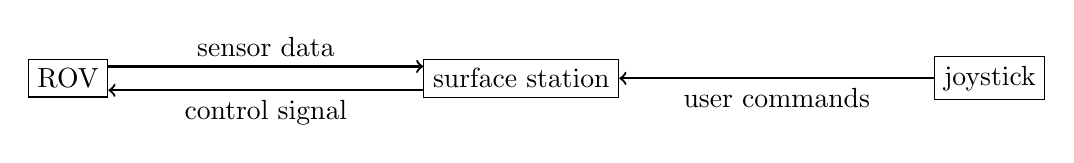
\begin{tikzpicture}[node distance = 4cm, auto]
      % Place nodes
      \node [rectangle, draw] (rov) {ROV};
      \node [right= of rov, rectangle, draw] (ss) {surface station};
      \node [right= of ss, rectangle, draw] (joy) {joystick};
      % Draw edges
      \path [->, thick] ([yshift=1ex]rov.east) edge node {sensor data} ([yshift=1ex]ss.west);
      \path [->, thick] ([yshift=-1ex]ss.west) edge node {control signal} ([yshift=-1ex]rov.east);
      \path [->, thick] (joy) edge node {user commands} (ss);
  \end{tikzpicture}
\caption[CoopROV data-flow diagram]{Block diagram of high-level data flow between different components in CoopROV}
\label{fig:cooprov_dataflow}
\end{figure}


\subsection{Hardware}

The exterior shell of CoopROV is composed of an acrylic frame that holds all housing tubes together. There are 3 housing tubes in total: an electronics tube, a connector tube and a battery tube. A \gls{cad} model of CoopROV in Figure~\ref{fig:cooprov_cad} illustrates the position of the housing tubes on the CoopROV frame. The electronics tube is a long transparent acrylic tube that holds all sensors and most electronics of the robot. The connector housing tube is a relatively short transparent acrylic tube with a molex connector plug inside it. This connector tube serves as a water proof connector plug that allows to change the sensor package by swapping out the electronics tube. The battery tube is a PVC pipe that holds 11.1 V Li Ion batteries. The clips and clamps that hold the tubes in place were made out of 3D-printed plastic parts. One big design improvement over OpenROV is the water proof seals. The waterproof seals comprise a delrin end cap with an O-ring seal along with 3 threaded rods to maintain 
the tension between the end caps and the acrylic tube. 
%
\begin{figure}	
    \centering
    \begin{subfigure}[]{0.33\textwidth}
        \centering
        \includegraphics[width=0.95\linewidth]{cooprov_frontview}
        \caption{Front view}
        \label{fig:cooprov_frontview}
    \end{subfigure}%
    \begin{subfigure}[]{0.33\textwidth}
        \centering
        \includegraphics[width=0.95\linewidth]{cooprov_sideview}
        \caption{Side view}
        \label{fig:cooprov_sideview}
    \end{subfigure}%
    \begin{subfigure}[]{0.33\textwidth}
        \centering
        \includegraphics[width=0.95\linewidth]{cooprov_isobackview}
        \caption{Isometric view (back)}
        \label{cooprov_isobackview}
    \end{subfigure}
    \begin{subfigure}[]{0.7\textwidth}
        \centering
        \includegraphics[width=0.95\linewidth]{cooprov_labels}
        \caption{Isometric view (front)}
        \label{cooprov_labels}
    \end{subfigure}
    \caption[CoopROV CAD model]{Different views of the CoopROV \gls{cad} model with some labeled parts}
    \label{fig:cooprov_cad}
\end{figure}

\subsection{Electronics}

The electronic components inside the electronics tube are responsible for controlling the thrusters and relaying the sensor data back to the surface station. The RaspberryPi and the surface station together constitute a distributed \gls{ros} system. For communication purposes, a \gls{tcp} link is established between the RaspberryPi and the surface station via the tether cable. The Arduino is connected to the RaspberryPi via the serial bridge and behaves like a node on the \gls{ros} system. The Arduino logs the data from the depth sensor and the \gls{imu}. Additionally, the arduino is also responsible for translating the motor commands into signals for the motor driver. Image data acquisition from the stereo camera is directly handled through a usb interface on the RaspberryPi.

There are two parallel data streams. One enables the flow of control commands throughout the system and other handles the data being logged from the various sensors. The control commands from the joystick flow through the surface station and RaspberryPi to reach the Arduino. The Arduino translates these motor velocity commands into \gls{pwm} signals, that enable the motor driver to run the propellers. The sensor data logged by the Arduino and RaspberryPi are served to other nodes on the \gls{ros} system through a \emph{publish-subscribe} communication paradigm \cite{eugster}. The block diagram in Figure~\ref{fig:cooprov_electronics} provides a graphical overview of the connections between the major electronic components on CoopROV. It is important to note that only one motor and motor driver are shown in Figure~\ref{fig:cooprov_electronics}, but in the actual system, there are 3 motors with dedicated motor drivers. Figure~\ref{fig:cooprov_electronics} also shows the two power supplies in the system. More details 
on the power supply components can be found in next section.

\begin{figure}
\centering
% Define block styles
\tikzset{
    block/.style={
        rectangle,
        draw,
        text width=10em,
        text centered,
        rounded corners
    },
    rectangle_connector/.style={
        to path={(\tikztostart) -- ++(#1,0pt) \tikztonodes |- (\tikztotarget) },
        pos=0.5
    },
    rectangle connector/.default=-2cm,
}
  \begin{tikzpicture}[auto]
      % Place nodes
      \node [rectangle, draw] (ps5) {Power supply 5V};
      \node [above right= of ps5, rectangle, draw] (rpi) {RaspberryPi};
      \node [below= of rpi, rectangle, draw] (ard) {Arduino};
      \node [right= of rpi, rectangle, draw] (stereo) {Stereo camera};
      \node [above right= 0.01cm and 1.4cm of ard, rectangle, draw] (depth) {Depth sensor};
      \node [below right= 0.01cm and 1.4cm of ard, rectangle, draw] (imu) {IMU};
      \node [below= of ard, rectangle, draw] (motdr) {Motor driver};
      \node [below= of motdr, rectangle, draw] (ps11) {Power supply 11.1V};
      \node [right= of motdr, rectangle, draw] (mot) {Thruster};

      % Draw edges
      \draw [rectangle_connector=2cm,->,thick] (ps5) to node {} (rpi);
      \draw [rectangle_connector=2cm,->,thick] (ps5) to node {} (motdr);
      \draw [rectangle_connector=1.5cm,<-,thick] (ard) to node {} (depth);
      \draw [rectangle_connector=1.5cm,<-,thick] (ard) to node {} (imu);
      \path [->, thick] (stereo) edge node {} (rpi); 
      \path [->, thick] (ps5) edge node {} (ard);
      \path [->, thick] (motdr) edge node {} (mot);
      \path [->, thick] (ps11) edge node {} (motdr);
      \path [->, thick] (ard) edge node {} (ard|-motdr.north);           
      \path [<-, thick] ([xshift=-1ex]ard.north) edge node {} ([xshift=-1ex]ard.north|-rpi.south);
      \path [->, thick] ([xshift=1ex]ard.north) edge node {} ([xshift=1ex]ard.north|-rpi.south);
  \end{tikzpicture}
  \caption[CoopROV electronics schematics]{Block diagram depicting the connectivity between major components in the electronics schematics}
  \label{fig:cooprov_electronics}
\end{figure}

\subsection{Power Supply} \label{sec:cooprov_power}

Power supply is a critical part of any robotic system. Almost all mobile robotic systems require batteries onboard. However tethered systems like the \gls{rov}s can have an alternative resource in form of power supply through the tether. Running power through a tether comes with its own set of challenges. \gls{dcp} transmitted at low voltages result in significant voltage drop due to the impedance of the long tether cables. Conversely using AC power at high voltages circumvents this problem but then runs into the need for onboard transformer/rectifier to transform the input \gls{acp} power into usable \gls{dcp} form. 

A robot's power supply components ought to be chosen, such that they can handle the expected operational load (also transients). For CoopROV, several power supply systems were tested. Four different battery types were evaluated: alkaline C, lithium ion, lithium phosphate and \glsfirst{lipo}. Tests revealed that the high transient current requirements ($>$20A) of CoopROV were only met by the \gls{lipo} composition. Thus, two sets of \gls{lipo} batteries were used to independently power the motors and electronics. This physical isolation of the power sources improves stability of the robot's power supply system and prevents electronic components from being affected by occasional erratic power draws of motors. More information on the two power sources is given in Table~\ref{tab:cooprov_battery}.

The two independent power sources (Table~\ref{tab:cooprov_battery}) cater to different sub-systems of CoopROV. The 5V power source drives all the onboard electronics. Additionally, the 5V power supply is stepped-down and regulated to protect the electronic circuits against voltage variations.  The 11.1V  (unregulated) power source meets the power demands of the motors. Figure~\ref{fig:cooprov_electronics} shows the different power supplies along with the different components powered by them. An approximate running time of the \gls{rov} is 1 hour 
can be obtained by doubling the number of \gls{lipo} batteries on each power source.
%
\begin{table}
\centering
\caption{CoopROV Battery Specifications}
  \begin{tabular}{lll} 
  \toprule
  Power Source	&Battery Specification\\
  \midrule
  11.1V	&\gls{lipo} 3-cell 11.1V 5400mAh\\
  5V	&\gls{lipo} 2-cell 7.4V 800mAh\\
  \bottomrule
  \end{tabular}
  \label{tab:cooprov_battery}
\end{table}


\subsection{Sensors}

CoopROV comes with 4 sensors; namely, stereo cameras, \gls{imu}, depth sensor and voltage sensors. A low-cost off-the-shelf Minoru 3D webcam \cite{minoru} was used to capture stereo images at 5 \gls{fps} with a resolution of $320\times 240$. The 9-\gls{dof} \gls{imu} on the robot provides instantaneous acceleration in the $x$,$y$ and $z$ directions along with roll, pitch and yaw. The depth sensor measures the water pressure and temperature to compute the robot's operating depth. The voltage sensors are connected on to the \gls{lipo} batteries to measure and report the instantaneous battery voltage. They also double as a protection to the \gls{lipo} batteries; they signal an alarm if the battery voltage drops below a critical value.

\subsection{Software}

The software of CoopROV is built on a \gls{ros} architecture. The different core functions of the robot are sub-divided into independent modules or \emph{\gls{ros}-nodes}. Each \gls{ros}-node has a specific task and can communicate with the other \gls{ros}-nodes. Additionally, the \gls{ros} architecture allows \gls{ros}-nodes running on different systems to communicate seamlessly: agnostic to where they are running. The interaction between different \gls{ros}-nodes is handled through a \emph{publish-subscribe} communication paradigm \cite{eugster}. These characteristics of the distributed \gls{ros} system was exploited to build CoopROV's software stack. The CoopROV setup comprises a distributed \gls{ros} architecture, where different \gls{ros}-nodes run either on the RaspberryPi or the surface station. Both these platforms are connected via a \gls{tcp} link. The different nodes running on the robot and the surface station along with their functionality is explained in the software architecture diagram in Figure~\ref{fig:cooprov_software}.
%
\begin{figure}
  \centering
  \includegraphics[width=0.9\textwidth]{cooprov_software}
  \caption[CoopROV software architecture]{CoopROV software architecture showing all the \gls{ros}-nodes along with a brief overview on their functionality}
  \label{fig:cooprov_software}
\end{figure} 


\section{Test Infrastructure}

Initial waterproofing tests were performed in the University of Delaware indoor swimming and diving pools. Later integration tests for software and electronics along with some experimental runs were performed in a circular tank at \gls{rdl} in University of Delaware.


\section{Localization Experiments}

Preliminary localization experiments were performed by placing an \gls{ar}-tag on the bottom of the water tank. Images from the stereo camera were used to detect and track the \gls{ar}-tag. Further experiments were performed by fusing the the 6-\gls{dof} position obtained from the \gls{ar}-tag localization and \gls{imu} values. Since there was no reliable reference measure to compare the reported position of the \gls{rov}, the quality of the results were not verified.


\section{Conclusion}

CoopROV was built as a research platform to conduct underwater object recognition and control experiments. It offers a low-cost solution with a easily reconfigurable hardware and extensible \gls{ros}-software interface. \gls{ros}-software support allows the robot to use open source perception and control algorithms available as a part of \gls{ros} software infrastructure. The sensor package comprising a stereo camera, \gls{imu} and depth sensor can be leveraged for object recognition and motion control experiments. The capabilities of the CoopROV system can be easily expanded to suit any research experiment like the multi-layered scallop recognition (Chapter~\ref{chap:scallop_recog}) and the multi-view object recognition (Chapter~\ref{chap:distdes}) discussed in this dissertation.


%=========================================================================================
% Conclusion

\chapter{Conclusions and Outlook}
\label{chap:thesis_conclusion}

%=========================================================================================

The work in this dissertation offers robotic image analysis tools designed to operate in noisy natural environments. 
Underwater environment is the primary domain used to validate these tools.
The two applications that drove the design of these object recognition tools are the automated subway car recognition and scallop recognition problems.
Additionally, a multi-view object classifier, that can operate in noisy images without segmentation, is also proposed.
Finally, an low cost \gls{rov}, CoopROV, was built to facilitate underwater experiments. The different insights gleaned from development of each of these tools will be discussed in the remainder of this section.

Chapter~\ref{chap:eigen} showcases the application of eigen-value based shape descriptors to the subway car recognition problem. 
Eigen-value based shape identification is a tool that can be used to identify simple geometric shapes. 
By reducing subway car recognition to rectangle matching, eigen-value based shape descriptor was
successful in recognizing subway cars from seabed images.
Though shape matching can aid object recognition, other cues like texture can often play an important role
in distinguishing an object. Since eigen-value shape descriptors only use shape information, 
they are not suited for applications where non-shape cues are more relevant in encoding object information. 
Additionally, while evaluating eigen-value shape descriptors, it was determined that 
discretization errors and segmentation errors can significantly impair the performance of eigen-value based shape descriptors.
Therefore, eigen-value shape descriptors is a useful tool for identifying
objects, provided we can guarantee that the shape of the object can be represented with minimal discretization error. 
Furthermore, for this method to work, the objects
we are interested in should exhibit a shape profile that is significantly different from
all other objects in the background. These requirements are very restrictive, and render recognition tasks involving 
complex shapes problematic. One such challenging problem is scallop recognition.
The visual cues presented by a scallop comprise its distinguishing crescent profile, along with its unique representative texture.
Since eigen-value descriptors neither handle complex shape profiles like crescents, nor do they capture textural information,
a more refined approach is warranted.
This led to the development of multi-layered object recognition framework proposed in Chapter~\ref{chap:scallop_recog}.

Marine biologists and oceanographers often depend on large natural image datasets to study benthic phenomenon. With the availability of robotic imaging vehicles, that generation datasets ranging millions of images are becoming increasingly common. Automated image processing tools are necessary to deal with such large image datasets. Most existing techniques are built on restrictive assumptions that do not generalize to noisy natural image datasets. The multi-layered object recognition approach described in Chapter~\ref{chap:scallop_recog} addresses this problem by providing researchers with a modular architecture that can scale to large natural image datasets. Modular architectures also contains the built-in flexibility to be reconfigured to solve varied object recognition problems.
This multi-layered framework was tasked with automated scallop recognition from \gls{auv} images, as a means to study scallop population. 
% This approach offers a hands-off automated alternative to manual enumeration that was also performed as a part of the scallop survey discussed in Chapter~\ref{chap:scallop_recog}.
% This four-layered automated scallop recognition framework combined a series of off-the-shelf computer vision tools like visual attention and graphcut, 
% along with custom designed noise filters and machine learning classifiers.
This framework was successful in recognizing 60\% of scallops in a dataset of over 8000 images.
The uniqueness of this approach lies in its ability to handle noisy natural images under varied environmental conditions.
To improve the performance of the classifier proposed here, and thereby reduce false positives, more information about a target object can be helpful.
To inject this additional information into the classification process, a multi-view object recognition algorithm discussed in Chapter~\ref{chap:distdes} was formulated.

The multi-view approach discussed in Chapter~\ref{chap:distdes} is machine learning 
technique designed for binary classification tasks. 
The objective here is to formulate a robust object classifier even in case of noisy image data.
Since noisy single-views of an object might often not contain sufficient information to unambiguously recognize it, information from multiple views are combined 
here to build a machine learning classifier. 
In this approach, the information from 13 images of each object specimen, captured from different heights, is encoded into a single object model.
Another salient character of this approach is the use of histogram-based global feature descriptors that do not
require segmentation of object pixels. Since segmentation can be challenging in noisy natural images, the lack of need for segmentation greatly boosts the appeal of this method. This method is evaluated on a combined dataset of 22 specimens comprising oranges and strawberries specimens.
All the specimens are correctly classified. Despite the small dataset of 22 images used, the exceptional performance of this classifier in noisy underwater data is encouraging. To decrease false positives, an approach like this could be used as a classification layer in a multi-layered approach, like the one described in Chapter~\ref{chap:scallop_recog}.

To collect data in underwater environments, a submersible robotic vehicle is often required.
Most commercially available robotic vehicles are either expensive or difficult to customize for research needs. To address this problem, CoopROV, a low cost \gls{rov} was designed as a research prototype to support underwater experiments. CoopROV carries an \gls{imu}, stereo cameras, depth and pressure sensors. The onboard electronics on the robot allows easy inclusion of new sensors. CoopROV also offers a \gls{ros} software interface that allows easy access to plethora of existing software tools. The low cost, and innate flexibility to modify the software and hardware, makes CoopROV an ideal platform to support underwater experiments.

There are some possible directions to extend the object recognition tools proposed in this dissertation. For instance the scallop recognition effort in Chapter~\ref{chap:scallop_recog} could benefit from using more descriptive 
templates. In Chapter~\ref{chap:scallop_recog}, we see that the appearance of a scallop is characterized by two crescents near the scallop rim: one bright and one dark. Currently, only the position of a dark crescent is captured by the templates used. Using templates that capture additional information, like the position of the bright crescent could be interesting. As for the multi-view object recognition method discussed in Chapter~\ref{chap:distdes}, a more expansive dataset could be used to test this algorithm. Another possible improvement is to generalize this multi-view algorithm to accept images from any series of heights instead of a fixed set of heights. Easing the restrictions on the different views needed by the multi-view algorithm could make the experiments and data collection effort easier. This multi-view approach could also be expanded to multi-class classification for dealing with more than 2 object classes. The CoopROV frame could be redesigned to improve the trim (weight distribution) of 
the vehicle. Designing controllers and building a localization system are other avenues where future improvements on CoopROV is possible.

This dissertation offers object recognition tools designed to work on noisy natural images. Each of these tools have been validated on different underwater applications. The developments here are intended to provide automated solutions to researchers dealing with large natural image datasets.
The availability of modular reconfigurable architectures to allow researchers to build custom solutions to solve their object recognition needs is the prime objective. The techniques proposed here are first steps in providing tools capable of handling noisy natural images. Further exploration on this domain is necessary to build more robust architectures that can recognize multiple classes of objects. Some examples of object recognition applications like subway car and scallop recognition are not all encompassing but provide an initial thrust in this domain. Further work to build extensive tools required by the marine research community is warranted. The overarching goal of this dissertation is to contribute to the object recognition 
tools available to strengthen the perception capabilities of robots. Ultimately, better scene understanding and perception abilities allow robotic systems to move towards autonomy.



%
% This is the Bibliography file (bibtex.tex)
% This generally works for BibTeX

% Use sample.bib for BibTeX database
\bibliography{thesis_ref}
% BibTeX style (plain, alpha, unsrt)
\bibliographystyle{plain}

                                      
\printglossary[type=\acronymtype]                  
                          
\end{document}